\documentclass[a4paper,11pt]{ltjsarticle}

% ========== package ========== %
% --- 数式環境 --- %
\usepackage{amsmath}
\usepackage{amssymb}
\usepackage{mathtools}
% --- 数式環境 END --- %
% ブラケット
\usepackage{braket}
% ベクトルの太文字
\usepackage{bm}
% 添え字左右上下 \fourIdx{左上}{左下}{右上}{右下}{ベース} で使う．Iは大文字
\usepackage{fouridx}
% 色
\usepackage{color}
% 余白指定
\usepackage{geometry}
% --- ページ内リンク --- %
\usepackage{hyperref}
\hypersetup{colorlinks=true,linkcolor=blue}
% --- ページ内リンク END --- %
% 花文字
\usepackage{mathrsfs}
% 画像
\usepackage{graphicx}
% tcolorbox
\usepackage{tcolorbox}
% appendix
\usepackage{appendix}
% --- 参考文献 --- %
\usepackage{etoolbox}
\usepackage{fontspec} % fontspecは読み込んでOKですが、設定順序に注意が必要です
%% --- 参考文献フォント --- %%
  \IfFontExistsTF{Times New Roman}{
    \newfontfamily\bibfontface{Times New Roman}
  }{
    \newfontfamily\bibfontface{FreeSerif} % 代替フォント
  }
%% --- 参考文献フォント END --- %%
%% --- 参考文献リンク位置 --- %%
  \BeforeBeginEnvironment{thebibliography}{%
    \phantomsection
    \addcontentsline{toc}{section}{参考文献}
  }
  \AtBeginEnvironment{thebibliography}{%
    \normalfont\bibfontface
  }
%% --- 参考文献のリンク位置 --- %%
% --- 参考文献 END --- %
% ========== package END ========== %

% ========== newcommand ========== %
% --- セクションから目次へのリンク --- %
\newcommand{\sectionlink}[1]{\section[#1]{\hyperlink{toc}{#1}}}
\newcommand{\subsectionlink}[1]{\subsection[#1]{\hyperlink{toc}{#1}}}
% セクション番号リンク
\makeatletter
\renewcommand{\@seccntformat}[1]{%
  \protect\hyperlink{toc}{\csname the#1\endcsname}\quad
}
\makeatother

% 原文との照合のため，式番号は原文の通し番号と付録番号を保持する．
% ==========- newcommand END ========== %
\allowdisplaybreaks
%===========================================================
% --- タイトル --- %
%===========================================================
\geometry{left=25mm, right=25mm, top=30mm, bottom=30mm}

% 原文の記号，引用，演習環境を再現する最小限の追加設定
\usepackage[numbers,sort&compress]{natbib}
\usepackage[hang,small,bf]{caption}
\usepackage{rotating}
\DeclareRobustCommand{\SkipTocEntry}[4]{}
\def\beq{\begin{equation}}
\def\eeq{\end{equation}}
\def\bea{\begin{eqnarray}}
\def\eea{\end{eqnarray}}
\def\Mp{M_{\rm pl}}
\def\d{{\rm d}}
\def\R{{\cal R}}
\def\l{\ell}
\newtheorem{thm}{演習}
\newtheorem{thmP}{問題}
\renewcommand{\theequation}{\arabic{equation}}
\renewcommand{\theHequation}{\arabic{part}.\arabic{section}.\arabic{equation}}
\setlength{\emergencystretch}{3em}
\hypersetup{pdftitle={インフレーションに関するTASI講義（日本語訳）},pdfauthor={Daniel Baumann},unicode=true}
\title{\bfseries インフレーションに関するTASI講義}
\author{Daniel Baumann\\
{\small ハーバード大学物理学科，Cambridge, MA 02138, USA}\\
{\small プリンストン高等研究所自然科学部門，Princeton, NJ 08540, USA}}
\date{\small 原文PDF表記：2024年11月26日\\arXiv第2版：2012年11月30日}

\begin{document}
\maketitle
% 原文の引用番号を維持するため，原文の文献順を明示する．
\nocite{Guth:1980zm,Linde:1981mu,Albrecht:1982wi,Hubble,abc,DickeCMB,WhitePaper,Dodelson,Mukhanov,WeinbergCosmology,WMAP5,unionsn,BassettReview,PaoloEFT,WeinbergEFT,BMReview,Shafi:2006cs,LythRiotto,WandsMulti,Bardeen:1980kt,BST,Wands:2000dp,Acquaviva02,malda,BD,Jacobson:2003vx,Lyth,WayneHu,CMBFAST,CAMB,NGreview,Kamionkowski:1996ks,Zaldarriaga:1996xe,NewmanPenrose,spergel/zaldarriaga:1997,Dodelson:2003ip,EPIC,BBKS,EisensteinHu,Steinhardt:2002ih,Steinhardt:2001st,Buchbinder:2007ad,Smith:2009jr,Nflation,MSW,Silverstein:2008sg,KKLMMT,Baumann:2007ah,Baumann:2008kq,Conlon:2005jm,BlancoPillado:2006he,BauZal,Babich_etal_04,BMRmulti,Bernardeau:2002jy,Bernardeau:2002jf,Sasaki:2008uc,Naruko:2008sq,Byrnes:2008wi,Byrnes:2006fr,Langlois:2008vk,Valiviita:2008zb,Assadullahi:2007uw,Valiviita:2006mz,Vernizzi:2006ve,Allen:2005ye,Linde:1996gt,Lyth_etal03,Dvali:2003em,Kofman:2003nx,Creminelli:2007aq,Koyama_etal07,Buchbinder_etal07,Lehners:2007wc,Lehners:2008my,Koyama:2007ag,Koyama:2007mg,Alishahiha:2004eh,GhostInflation,Senatore:2004rj,Creminelli:2003iq,Chen:2006nt,Gordon:2000hv,Lyth:2002my,Weinberg04b,Komatsu:2009kd,Schwinger:1960qe,Calzetta:1986ey,Jordan:1986ug,Weinberg:2005vy,komatsu01,Fergusson:2008ra,DBI,Holman:2007na,Creminelli:2004yq,Cheung:2007sv,Senatore:2009gt,BMR1,BMR2,Senatore:2008wk,Dalal:2007cu,Slosar:2008hx,Copeland:1994vg,PolchinskiOne,Polchinski,KKLT,Lyth:1996im,Linde:1983gd,Vafa:2005ui,Ooguri:2006in,Adams:2006sv,Hertzberg:2007ke,Douglas:2006es,KS,KT,GKP,Baumann:2006cd,Baumann:2006th,Baumann:2007np,Krause:2007jk,Nakahara,BaumannProgress,Firouzjahi:2005dh,ShanderaTye,Freese:1990rb,Banks:2003sx,Svrcek:2006yi,Easther:2005zr,Liddle:1998jc,Kallosh:2007cc,Grimm:2007hs,Hertzberg:2007wc,Flauger:2008ad,Caviezel:2008tf,Sarangi,CMP,Burgess:2007pz,Kallosh:2007ig,Linde:2005dd,McAllister:2007bg,Cline:2006hu,Flauger:2009ab,:2006uk,CMBPolWorkshop,Kosowsky:2004sw,Ruhl:2004kv,Taylor:2006jw,Samtleben:2008rb,Yoon:2006jc,Oxley:2005dg,MacTavish:2007kh,Bock:2009xw,Vilenkin:1983xq,Linde:1986fd,Linde:1993nz,Linde:1993xx,GarciaBellido:1993wn,Vilenkin:1994ua,Garriga:2005av,Bousso:2006ev,Linde:2007nm,Bousso:2008hz,DeSimone:2008if,Garriga:2008ks,Winitzki:2008jp,Linde:2008xf,Malik:2008im,LiciaStats,ADM,Seery:2007we,Adshead:2009cb}
\begin{center}
{\small 日本語訳：\href{https://arxiv.org/abs/0907.5424v2}{arXiv:0907.5424v2}\\
原題：TASI Lectures on Inflation}
\end{center}
\begin{abstract}
5回の連続講義を通じて，インフレーション宇宙論を概観する．まずFriedmann--Robertson--Walker（FRW）宇宙論における初期条件の問題を説明し，宇宙初期の加速膨張期であるインフレーションが，これらの問題をどのように解決するかを述べる．次に，インフレーションが微視的な量子揺らぎを宇宙の構造形成の巨視的な種へと変換する仕組みを説明する．スカラー揺らぎとテンソル揺らぎの原始スペクトルを求める有名な計算を，詳細に提示する．そのうえで，宇宙マイクロ波背景放射の揺らぎの観測からインフレーション期の情報を抽出するという逆問題を定式化する．インフレーションを支持する現在の観測的証拠と，今後の検証の可能性を論じる．最後に，弦理論におけるインフレーションを解説し，インフレーションを基礎物理と結びつける際の課題を概観する．
\end{abstract}

\paragraph{第1講：インフレーションの古典力学}
本講の目的は，インフレーション宇宙論の古典力学を第一原理から導入することである．基本的なFRW宇宙論を簡単に復習した後，従来のビッグバン理論が初期条件の問題をもたらすことを示す．すなわち，私たちが知るような宇宙は，非常に特殊で微調整された初期条件からしか生じない．次に，インフレーション，すなわち宇宙初期の加速膨張期がこの初期条件の問題を解決し，一般的な初期条件から私たちの宇宙が生じることを可能にする仕組みを説明する．インフレーションに必要な条件を述べ，インフレーションが時空の因果構造を変えることによって，ビッグバンの難問をどのように解決するかを説明する．最後に，インフレーション的膨張の物理的起源を論じて本講を終える．

\paragraph{第2講：インフレーション中の量子揺らぎ}
本講では，インフレーション中の量子揺らぎが生成する原始揺らぎスペクトルの有名な計算を復習する．計算をすべて詳しく示し，「ごまかし」や近似をできるだけ避ける．宇宙論的摂動論の基礎的な側面を簡単に復習した後，まず，インフレーションが微視的な量子揺らぎを宇宙の構造形成の巨視的な種へ変換する基本的な仕組みを定性的にまとめる．次いで，曲がった時空の場の量子論への教育的な導入として，単純な調和振動子の量子化を復習する．真空が最低エネルギー状態であることを要求すると，一意な真空状態が選ばれる点を強調する．その後，インフレーションに対する対応する計算を行う．スカラー揺らぎとテンソル揺らぎの両方のパワースペクトルを計算する．

\paragraph{第3講：観測との接点}
本講では，宇宙マイクロ波背景放射と大規模構造の観測から，インフレーションによる摂動スペクトルの情報を抽出するという逆問題を説明する．前講で計算したゲージ不変なスカラーおよびテンソルのパワースペクトルと，観測されるCMB異方性および銀河パワースペクトルの間の正確な関係を定義する．原始揺らぎと後期宇宙の観測量を関係づける伝達関数を示す．これらの結果を用いて，インフレーションを支持する現在の観測的証拠を論じる．最後に，今後インフレーションを検証する機会を示す．

\paragraph{第4講：原始非ガウス性}
本講では，原始非ガウス性の研究における主要な理論的結果をまとめる．結果の大部分は証明なしに述べるが，インフレーションの根本的な物理的起源を制約するうえでの意義を説明する．非ガウス統計の基本的な診断量としてバイスペクトルを導入した後，その運動量依存性がインフレーションの作用を探る強力な手段になることを示す．大きな非ガウス性は，インフレーション中にインフラトンの相互作用が重要である場合にのみ生じうる．したがって，単一場スローロール・インフレーションでは，非ガウス性は観測できないほど小さいと予言される一方，複数の場，高階微分相互作用，または非標準的な初期状態をもつ模型では，有意な大きさになりうる．最後に，原始非ガウス性を検出または制約する観測的な見通しを論じて本講を終える．

\paragraph{第5講：弦理論におけるインフレーション}
この連続講義を，やや発展的な話題である弦理論におけるインフレーションの議論で締めくくる．Liam McAllisterとの最近の総説に基づき，この主題を教育的に概観する．本講の中心的な主題は，インフレーションのPlanckスケールの物理に対する敏感さである．これこそが，弦理論でインフレーションを実現する主な動機であると同時に，中心的な理論課題でもあると論じる．これらの問題を，弦理論における2つのインフレーション・シナリオ，すなわちワープしたDブレーン・インフレーションとアクシオン・モノドロミー・インフレーションの事例を通じて説明する．最後に，理論と観測の両面で今後進展が期待される方向を示す．

\vspace{1em}
\noindent{\footnotesize 電子メール：\texttt{dbaumann@physics.harvard.edu}}
\setcounter{footnote}{0}
\clearpage
\hypertarget{toc}{}
\tableofcontents
\clearpage

\part{序論}

\vspace{0.7cm}
\begin{quote}
「チャイナタウンで道に迷わず歩くことさえ十分に難しいというのに，

宇宙を『知ろう』とする人たちには驚かされる」

{\it Woody Allen}
\end{quote}


\vspace{0.2cm}


 \begin{figure}[h!]
    \centering
        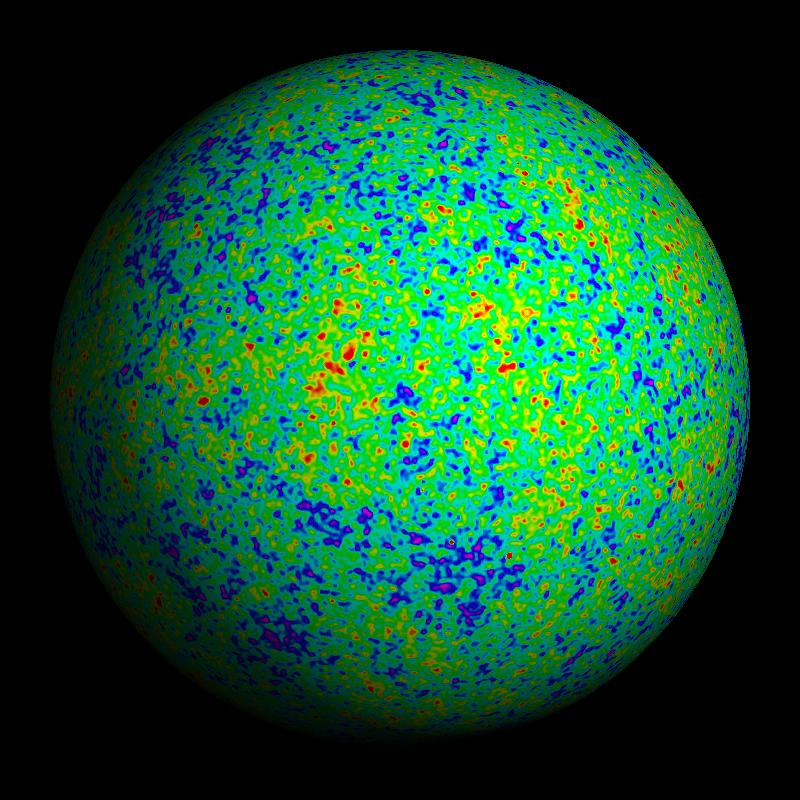
\includegraphics[width=.45\textwidth]{./CMB.jpg}
\caption{宇宙マイクロ波背景放射（CMB）の揺らぎ．何がこれを生み出したのだろうか．}
    \label{fig:CMB1}
\end{figure}
 

%\sectionlink{Introduction}
\sectionlink{構造の微視的起源}

\subsectionlink{TASI 2009：{\sl 大きなものと小さなものの物理}}

%{\tt more}

宇宙マイクロ波背景放射（CMB）の温度揺らぎ（図~\ref{fig:CMB1}参照）は，驚くべき物語を伝えている．現在ではウィルキンソン・マイクロ波異方性探査機（WMAP）などの実験によってほぼ日常的に測定されるようになったマイクロ波の天空の温度変動は，原始宇宙の密度に微小な揺らぎがあったことを物語っている．
これらの揺らぎは重力不安定性によって成長し，現在の宇宙で観測される大規模構造（LSS）になった．%of the late-time universe.
ビッグバンの熱的な残光の観測を，数十億年後の構造形成に結び付けることに成功した私たちは，さらに大胆な問いへと向かう．CMBの揺らぎの根本的な微視的起源は何だろうか．
この問いに答えることは，宇宙のあらゆる構造の物理的起源を根本から理解することにほかならない．

本講義では，宇宙の{\it インフレーション}期が，この構造の形成と進化の描像に不可欠な一部をなしていたという，現在最も有力な作業仮説を解説する．
インフレーション\cite{Guth:1980zm, Linde:1981mu, Albrecht:1982wi}とは極初期宇宙における指数関数的膨張の時期であり，ビッグバン特異点の約$10^{-34}$秒後に起こったと考えられている．
驚くべきことに，インフレーションは，宇宙の大域的な一様性と，私たちの銀河のような構造が形成される種となった小さな揺らぎの，両方を生み出したと考えられている．

この連続講義の中心となるのは，インフレーションが微視的な量子揺らぎを宇宙のエネルギー密度の巨視的な揺らぎへと変換した物理的機構を，詳しく説明することである．
この意味でインフレーションは，{\sl TASI 2009}の主題である「大きなものと小さなものの物理」のつながりを示す，最も劇的な例を与える．
インフレーションが生み出す揺らぎのスペクトルの統計的性質とスケール依存性を，具体的に計算する．この結果は，宇宙の構造形成を扱うすべての研究への入力となり，現代理論宇宙論の大きな成果の一つである．



\subsectionlink{宇宙の構造と進化}

宇宙の膨張には否定しようのない証拠がある．遠方の銀河からの光は，スペクトルの赤い側へ系統的にずれている\cite{Hubble}．軽元素（H，He，Li）の観測存在量は，ビッグバン元素合成（BBN）の予言と一致する\cite{abc}．そして，CMBについて説得力のある唯一の説明は，それが高温の初期宇宙から残った放射だというものである\cite{DickeCMB}．
 
 \begin{figure}[h!]
    \centering
        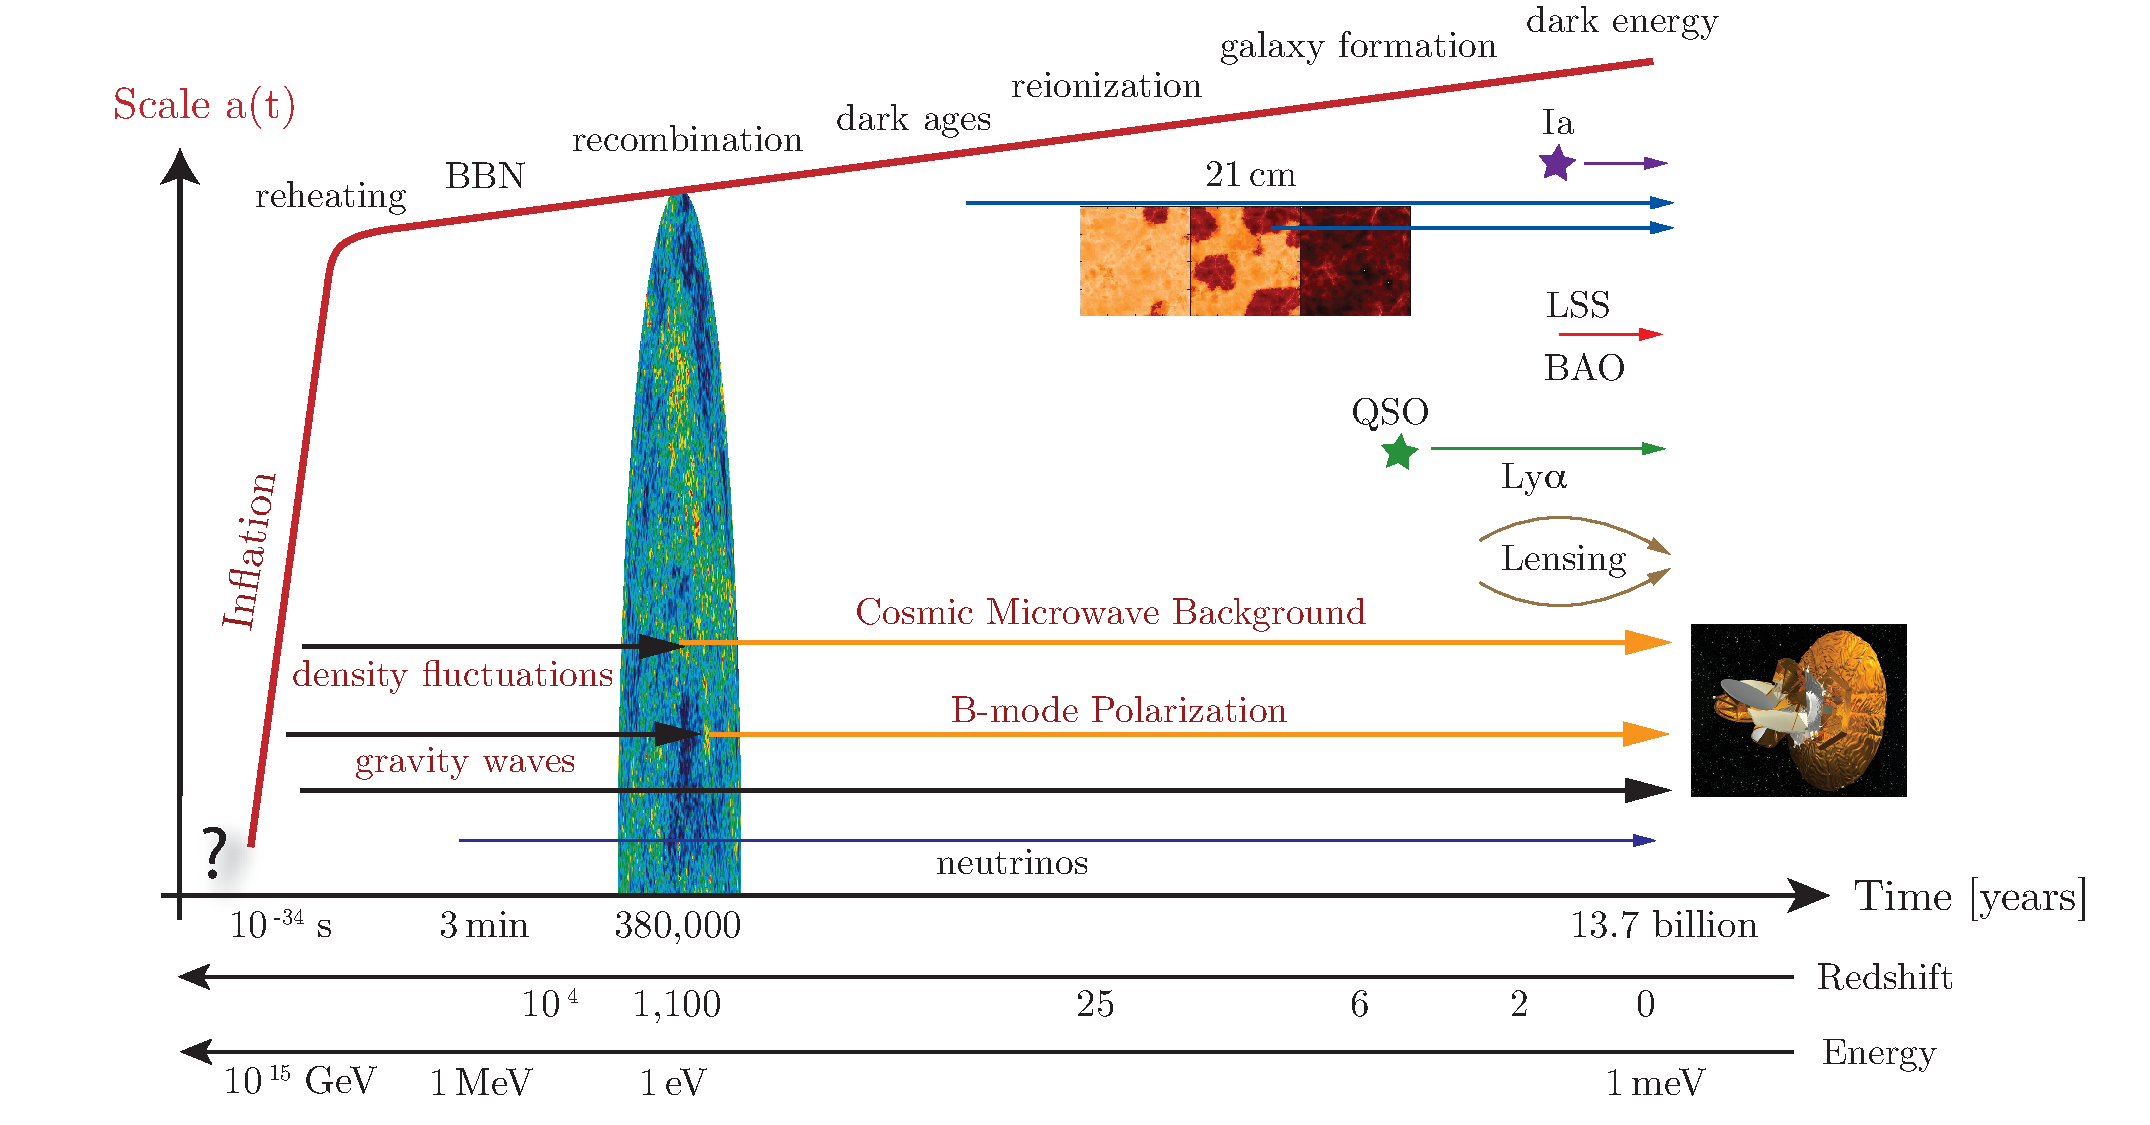
\includegraphics[width=1.0\textwidth]{./timeline}
\caption{宇宙の歴史．この模式図には，宇宙史の主要な出来事と，それに対応する時間およびエネルギースケールを示す．また，宇宙の構造と進化について情報を与える，いくつかの宇宙論的観測手段も示す．%\newline
{\small {\it 略語}：BBN（ビッグバン元素合成），LSS（大規模構造），BAO（バリオン音響振動），QSO（準恒星状天体＝クエーサー），Ly$\alpha$（ライマン・アルファ），CMB（宇宙マイクロ波背景放射），Ia（Ia型超新星），21cm（水素の21cm遷移）．}}
    \label{fig:timeline}
\end{figure}
 
膨張宇宙における熱力学と素粒子物理学を特徴付ける原理は二つある．
{\sl i)} 相互作用率が膨張率を下回ると，粒子間の相互作用が凍結すること，
{\sl ii)} 物理法則における破れた対称性は，高エネルギーで回復しうることである．
表~\ref{tab:timeline}に，宇宙の熱史と，対称性の破れに関係するさまざまな相転移を示す．
以下では，私たちの宇宙の進化を画するこれらの出来事を，定性的に簡潔に概観する．
この宇宙史のどの側面が確立された物理学に基づき，どの側面により推測的な考えが必要なのかを強調する．
% to celebrate the achievements of physics and cosmology in the past century.
%We will emphasize which aspects we consider certain and which are still more speculative.

\begin{table}[h!]
\caption{宇宙史の主要な出来事．}
\label{tab:timeline}
\begin{center}
\begin{tabular}{l | r | r | r}
 & {\small 時間} & {\small エネルギー} & \\
 \hline 
 \hline
 {\small プランク期？} & {\small $< 10^{-43}$ s} & {\small $10^{18}$ GeV} &\\
 {\small 弦スケール？} & {\small $\gtrsim 10^{-43}$ s} & {\small $\lesssim 10^{18}$ GeV} & \\
{\small 大統一？} & {\small $\sim 10^{-36}$ s} & {\small $10^{15}$ GeV} & \\
{\small インフレーション？} & {\small $\gtrsim 10^{-34}$ s} & {\small $\lesssim 10^{15}$ GeV} &\\
{\small 超対称性の破れ？} & {\small $< 10^{-10}$ s} & {\small $> 1$ TeV} &\\
{\small バリオン数生成？} & {\small $< 10^{-10}$ s} & {\small $> 1$ TeV} &\\
\hline
\hline
{\small 電弱統一} & {\small $10^{-10}$ s} & {\small 1 TeV} &\\
{\small クォーク・ハドロン転移} & {\small $10^{-4}$ s} & {\small $10^2$ MeV} &\\
{\small 核子の凍結} & {\small 0.01 s} & {\small 10 MeV} &\\
{\small ニュートリノの脱結合} & {\small 1 s} & {\small 1 MeV} &\\
{\small BBN} & {\small 3 min} & {\small 0.1 MeV} &\\
\hline 
\hline
& & & {\small 赤方偏移} \\
\hline 
\hline
{\small 物質・放射等価} & {\small $10^4$ 年} & {\small 1 eV} & {\small $10^4$}\\
{\small 再結合} & {\small $10^5$ 年} & {\small 0.1 eV} & {\small 1,100}\\
{\small 暗黒時代} & {\small $10^5 - 10^8$ 年} & & {\small $> 25$} \\
{\small 再電離} & {\small $10^8$ 年} & & {\small $25 - 6$}\\
{\small 銀河形成} & {\small $\sim 6 \times 10^8$ 年} & & {\small $\sim 10$} \\
{\small ダークエネルギー} & {\small $\sim 10^9$ 年} & & {\small $\sim 2$} \\
{\small 太陽系} & {\small $8 \times 10^9$ 年} & & {\small 0.5} \\
{\small アルベルト・アインシュタイン誕生} & {\small $14 \times 10^{9}$ 年} & {\small 1 meV} & {\small 0} \\
\hline
\end{tabular}
  \end{center}
\end{table}

$10^{-10}$秒から現在までの宇宙史は，よく理解され，実験的に検証された素粒子物理学，原子核・原子物理学，および重力の法則に基づいている．
したがって，その間に宇宙を形作った出来事について，ある程度の確信を持つことには根拠がある．
% (see Figure~\ref{fig:timeline} and Table~\ref{tab:timeline}).

電弱相転移の時刻（$10^{-10}$\,s），$100$ GeVの宇宙に入ってみよう．
$100$ GeVより上では電弱対称性が回復し，$Z$および$W^\pm$ボソンは質量を持たない．
相互作用は，クォークとレプトンを熱平衡に保つのに十分強い．
$100$ GeVより下では，電磁力と弱い力の間の対称性が破れ，$Z$および$W^\pm$ボソンは質量を獲得する．そして宇宙の温度の低下とともに，弱い相互作用の断面積が減少する．
その結果，$1$ MeVでニュートリノは他の物質から脱結合する．
その直後の$1$秒には，温度が電子の静止質量を下回り，電子と陽電子が効率よく対消滅する．初期に存在した10億分の1の物質・反物質非対称性だけが生き残る．
こうして生じた光子・バリオン流体は平衡状態にある．
$0.1$ MeV付近で強い相互作用が重要になり，ビッグバン元素合成（$\sim 200$\,s）の間に陽子と中性子が結合して軽元素（H，He，Li）を形成する．H，He，Liの存在量の予言が成功したことは，ビッグバン理論の最も目覚ましい帰結の一つである．
物質密度と放射密度は$1$ eV（$10^{11}$\,s）付近で等しくなる．
プラズマ中では，荷電した物質粒子と光子が強く結合しており，密度の揺らぎは宇宙の「音波」として伝播する．
$0.1$ eV付近（38万年）で陽子と電子が結合して，中性の水素原子となる．
光子は脱結合し，自由に伝播する宇宙マイクロ波背景放射を形成する．
137億年後，これらの光子は宇宙の最も古いスナップショットを私たちに届ける．
CMB温度の異方性は，原始物質密度の揺らぎの証拠を与える．
% of the early universe.

これらの小さな密度摂動$\rho({\bf x}, t) = \bar \rho(t) [1+ \delta({\bf x}, t)]$は，重力不安定性によって成長し，後期宇宙で観測される大規模構造を形成する．
背景の圧力と普遍的な重力の引力との競合が，構造の成長の詳細を決める．
放射優勢期の成長は遅く，$\delta \sim \ln a$である（ここで$a(t)$は空間の膨張を記述するスケール因子）．物質が背景密度を支配するようになると（圧力がゼロに下がり），集積はより効率的になり，$\delta \sim a$となる．まず小さなスケールが非線形化し，$\delta \gtrsim 1$となって，全体の膨張から切り離された重力的に束縛された天体を形成する．
これによって，まず小さなスケールの構造（恒星や銀河など）が形成され，次いで合体してより大きな構造（銀河団や超銀河団）になるという，階層的構造形成の描像が得られる．
赤方偏移$z \sim 25$（$1+z = a^{-1}$）付近で，最初の恒星からの高エネルギー光子が銀河間物質中の水素を電離し始める．この「再電離」の過程は$z \approx 6$で完了する．
一方，最も大質量の恒星は核燃料を使い果たし，「超新星」として爆発する．
これらの爆発の中で，生命の形成に必要な重元素（C，O，\dots）が作られる．これが「私たちは皆，星屑でできている」という言葉の由来である．
$z \approx 1$では，負の圧力を持つ「ダークエネルギー」が宇宙を支配するようになる．
背景時空の膨張は加速し，構造の成長は止まって，$\delta \sim$一定となる．


\subsectionlink{最初の$10^{-10}$秒}

$10^{-10}$秒（1~TeV）から現在までの宇宙史は，観測事実と，素粒子物理学の標準模型，一般相対性理論，流体力学などの検証済みの物理理論に基づく．例えば，高エネルギー物理学の基本法則は，現在の粒子加速器が到達するエネルギー（$\sim 1$~TeV）まで十分に確立されている．
$10^{-10}$秒より前には宇宙のエネルギーが1~TeVを超え，実験が直接導いてくれるという安心感を失う．
したがって，この時代の物理学は，魅力的であるのと同じくらい推測的でもある．

CMB温度に見られる揺らぎを説明するには，種となる原始揺らぎを入力しなければならない．
本講義では，これらの原始揺らぎが極初期宇宙（$\sim 10^{-34}$秒）のインフレーション期に生成されたという仮説を説明する．
エネルギー密度の微視的な量子揺らぎが，インフレーションによる膨張によって，その時点の物理的な地平線よりも大きな巨視的スケールへ引き伸ばされる様子を説明する．
摂動が地平線の外に出ると，因果的な物理過程はそれに影響を与えられなくなる．振幅が一定のまま凍結され，その後の通常の（加速しない）ビッグバン膨張の間に，地平線へ再び入るまでその状態が続く．宇宙の構造に対応する揺らぎは，CMB光子が脱結合する少し前，宇宙年齢が約10万年のときに地平線へ再突入する．
地平線の内部では因果的な物理過程が摂動の振幅に影響を与えることができ，実際にそれがCMBの音響ピーク構造や，高密度の揺らぎが銀河・銀河団へと崩壊する過程をもたらす．
地平線への再突入後の摂動の進化は理解されており，計算することもできるため，後期のCMBやLSSの観測から，入力となった原始スペクトルを推定できる．
このスペクトルがインフレーションによって生成されたと仮定すると，それは宇宙年齢が$10^{-34}$秒であったときの物理的状況を観測的に探る手段となる．
宇宙論を用いて最高エネルギーの物理を探る，この魅力的な可能性が本講義の主題である．

\sectionlink{講義の構成}

{第1講}では，インフレーションの{\it 古典的}な背景力学を導入する．インフレーションが地平線問題と平坦性問題をどのように解決するかを説明する．スローロール条件と再加熱を論じ，インフレーションによる膨張の物理的起源を考察する．
{第2講}では，インフレーション中の{\it 量子}揺らぎが，大規模構造の形成の種となる仕組みを説明する．スカラー摂動とテンソル摂動$\R$および$h_{ij}$のインフレーションによるパワースペクトルを，詳細に導出する．
{第3講}では，第2講の結果を，宇宙マイクロ波背景放射と銀河分布の観測に結び付ける．つまり，天空で$P_\R(k)$と$P_h(k)$をどのように測定するかを説明する！ 現在の観測的制限を述べ，将来のインフレーションの検証を強調する．
{第4講}では，原始揺らぎの非ガウス性の研究における主要な結果を示す．
非ガウス相関から，インフレーションの作用に関する重要な情報がどのように得られるかを説明する．
{第5講}では，現在の研究の最前線にある発展的な話題，すなわち弦理論におけるインフレーションを扱う．
この主題の主要な難問を説明し，最近の進展をまとめる．
%primordial non-Gaussianity.

\vskip 5pt
各講義を自己完結的にするため，それぞれの中心部分に先立つ短い{\sl 復習}の節で，必要な背景知識を示す．
各講義の最後には，最も重要な結果の{\sl まとめ}を置く．
本文中の随所に現れる問題や演習と，講義の末尾に独立した{\sl 問題集}として付した長めの問題は，各講義の重要な一部である．
演習は，講義の内容を補完したり，計算の細部を補ったりするよう，注意深く選んである．

\vskip 5pt
いくつかの付録には，宇宙論的摂動論の標準的な結果と，インフレーション中の摂動計算の詳細をまとめた．これらの付録が，読者にとって有用な参照資料となることを願っている．
%In fact, in recent research projects I frequently found myself consulting these appendices, so I hope that they can be equally useful for others.

\newpage
\subsubsection*{記法}

本講義では，記法に一貫性と整合性を持たせるよう努めた．

全編を通じて，天与の自然単位系を用いる．
\beq
c = \hbar  \equiv 1\, . \nonumber
\eeq
換算プランク質量を次のように定義し，
\beq
M_{\rm pl} = (8 \pi G)^{-1/2}\, , \nonumber
\eeq
しばしばその値を1と置く．
計量の符号は$(-+++)$とする．
ギリシャ文字の添字は$\mu, \nu =0,1,2,3$の値を取り，ラテン文字の添字は$i,j=1,2,3$を表す．
フーリエ変換の規約は
\beq
\R_{\bf k} = \int \d^3 {\bf x}\, \R({\bf x}) e^{-i {\bf k} \cdot {\bf x}}\, , \nonumber
\eeq
とし，したがってパワースペクトルは
\beq
\langle \R_{\bf k} \R_{{\bf k}'} \rangle = (2\pi)^3 \delta({\bf k}+ {\bf k}') P_\R(k) \, , \qquad \Delta_\R^2(k) \equiv \frac{k^3}{2\pi^2} P_\R(k)\, . \nonumber
\eeq
である．共形時間には文字$\tau$を用いる（天体物理学で光学的厚さを表すパラメータと混同しないよう注意されたい）．文字$\eta$は第2スローロール・パラメータのために取っておく．物理的時間に関する微分は上付きのドットで表し，共形時間に関する微分はプライムで表す．
偏微分はコンマ，共変微分はセミコロンで表す．

\subsubsection*{謝辞}

素粒子物理学の理論高等研究所（{\sl TASI}）で本講義を行う機会を与えてくださったScott DodelsonとCsaba Csakiに，深く感謝する．

この数年間，師であるLiam McAllister，Paul Steinhardt，Matias Zaldarriagaと，共同研究者のIgor Klebanov，Anatoly Dymarsky，Shamit Kachru，Hiranya Peiris，Alberto Nicolis，Asantha Coorayから，多くのことを学んだ．
彼らが洞察を惜しみなく分かち合ってくれたことに感謝する．
{\sl CMBPol}インフレーション作業部会\cite{WhitePaper}のメンバーからの助言にも，大いに感謝している．
本講義で扱う多くの話題に関する彼らの専門的な意見は，私にとって極めて貴重であった．
Richard Easther，Eva Silverstein，Eiichiro Komatsu，Mark Jackson，Licia Verde，David Wands，Paolo Creminelli，Leonardo Senatore，Andrei Linde，Sarah Shanderaとの議論からも，多くのことを学んだ．

この講義録の執筆中に温かく迎えてくださったAspen Center for Physics，ボストンのTrident Cafe，ケンブリッジのDado Teaに感謝する．

最後に，質問によって私に挑み，この講義録の草稿に意見を寄せてくれた{\sl TASI 2009}の学生たちに感謝したい．
\newpage
\part{第1講：インフレーションの{\sl 古典的}力学}

\vspace{0.5cm}
 \hrule \vspace{0.3cm}
\begin{quote}
{\bf 要旨}

\noindent
本講義の目的は，インフレーション宇宙論の古典的力学を第一原理から導入することである．
基本的なFRW宇宙論を簡単に復習した後，通常のビッグバン理論が初期条件問題を生じることを示す．すなわち，私たちの知る宇宙は，極めて特殊で微調整された初期条件からしか生まれない．次に，インフレーション（初期の加速膨張期）がこの初期条件問題をどのように解決し，一般的な初期条件から私たちの宇宙が生じることを可能にするかを説明する．
インフレーションに必要な条件を述べ，インフレーションが時空の因果構造をどのように変えて，ビッグバンの謎を解くかを説明する．
最後に，インフレーションによる膨張の物理的起源を論じて本講義を締めくくる．
%We describe single-field slow-roll inflation, reheating, the UV sensitivity of models of inflation and inflation in string theory.
\end{quote}
\vspace{0.1cm}  \hrule
 \vspace{0.5cm}
 
 
%\sectionlink{Cosmological Preliminaries}
%\sectionlink{FRW Cosmology}
\sectionlink{{\sl 復習}：一様な宇宙}
\label{sec:FRW}

準備として，一様な宇宙の基本的な性質を復習する．
この内容は{\sl TASI 2009}におけるTurner教授の講義で扱われ，また宇宙論のどの教科書にも含まれているので（例えば\cite{Dodelson, Mukhanov, WeinbergCosmology}），ここでは簡潔に述べ，多くの概念は読者向けの演習を通じて思い出してもらうことにする．
当然ながら，インフレーションの研究に最も関係の深い事項に焦点を当てる．

\subsectionlink{FRW時空}

宇宙論は，最大のスケールにおける宇宙の構造と進化を記述する．大きなスケールで{\it 一様性}と{\it 等方性}\footnote{{\it 一様な}空間とは，並進不変，すなわちどの点でも同じである空間のことである．{\it 等方的な}空間とは，回転不変，すなわちどの方向でも同じである空間のことである．あらゆる点で等方的な空間は必ず一様であるが，逆は成り立たない．例えば，一様な電場のある空間は並進不変だが，回転不変ではない．}を仮定すると，宇宙の時空を表すフリードマン・ロバートソン・ウォーカー（FRW）計量に導かれる（{\bf 問題~\ref{pro:FRW}}参照）．
\beq
\label{equ:FRW}
\fbox{$\displaystyle
\d s^2 = - \d t^2 + a^2(t)  \left(\frac{\d r^2}{1-k r^2} + r^2 (\d \theta^2 + \sin^2 \theta \d \phi^2) \right) $}\, .
\eeq
ここでスケール因子$a(t)$は，異なる時刻における空間的超曲面$\Sigma$の相対的な大きさを特徴付ける．曲率パラメータ$k$は，$\Sigma$が正の曲率を持つ場合に$+1$，$\Sigma$が平坦な場合に$0$，$\Sigma$が負の曲率を持つ場合に$-1$である．
式~(\ref{equ:FRW})は共動座標を用いている．宇宙は$a(t)$の増加とともに膨張するが，銀河や観測者は，それらに力が働かない限り，すなわち固有運動がない限り，
%\footnote{This statement only applies to the Hubble flow and ignores the peculiar velocities of galaxies ${\bf v}_{\rm pec} = (\dot r, \dot \theta, \dot \phi)$.} 
座標$r$，$\theta$，$\phi$を一定に保つ．
対応する物理的距離はスケール因子を掛けて$R=a(t) r$と求められ，固有速度がゼロの天体であっても時間に依存する．
座標変換によって計量(\ref{equ:FRW})は次のように書ける．
\beq
\label{equ:FRW2}
\fbox{$\displaystyle
\d s^2 = - \d t^2 + a^2(t)  \left(\d \chi^2 + \Phi_k(\chi^2) (\d \theta^2 + \sin^2 \theta \d \phi^2) \right) $}\, ,
\eeq
ここで，
\beq
r^2 = \Phi_k(\chi^2) \equiv  \left\{
\begin{array}{c} \sinh^2 \chi \\ \chi^2 \\ \sin^2 \chi \\
\end{array} \right. \quad \begin{array}{l} k=-1 \\ k=0 \\ k=+1 \end{array}\, .
\eeq
%Here, $r$ and $\chi$ are
%{\it comoving coordinates}. They are related to physical coordinates by the scale factor.
FRWの仮定のもとで，一様な宇宙の進化は一つの関数$a(t)$に帰着する．
その形は，アインシュタイン方程式を通じて宇宙の物質内容によって決まる（\S\ref{sec:EinsteinEqns}参照）．
FRW時空を特徴付ける重要な量が，次の膨張率である．
\beq
\fbox{$\displaystyle
H \equiv \frac{\dot a }{a} $}\, .
\eeq
{\it ハッブル・パラメータ}$H$は時間の逆数の単位を持ち，膨張する宇宙では正（収縮する宇宙では負）である．
これはFRW時空の基本的なスケールを定める．すなわち，一様な宇宙の特徴的な時間スケールはハッブル時間$t\sim H^{-1}$であり，特徴的な長さスケールはハッブル長$d \sim H^{-1}$である（$c=1$の単位系）．ハッブル・スケールは宇宙年齢のスケールを定め，ハッブル長は観測可能な宇宙の大きさを定める．


\subsectionlink{運動学：共形時間と地平線}

宇宙の平均的な時空の計量を定義したので，光や物質粒子の伝播の運動学的性質を調べることができる．

%\vskip 6pt
%\noindent
\subsubsection*{共形時間とヌル測地線}

宇宙の因果構造は，FRW時空(\ref{equ:FRW})における光の伝播によって決まる．質量のない光子は，$\d s^2 = 0$を満たすヌル測地線に沿って進む．これらの光子の軌跡は，次のように共形時間\footnote{共形時間は，宇宙の膨張とともに進み方が遅くなる「時計」と解釈できる．}を定義すると，最も容易に調べられる．
\beq
\fbox{$\displaystyle
\tau = \int \frac{\d t}{a(t)} $}\, ,
\eeq
このときFRW計量は
\beq
\d s^2 =a(\tau)^2 \left[- \d \tau^2 +  \left(\d \chi^2 + \Phi_k(\chi^2) (\d \theta^2 + \sin^2 \theta \d \phi^2) \right) \right] \, .
\eeq
となる．等方的な宇宙では，次の2次元の線素で決まる，光の動径方向の伝播を考えればよい．
\beq
\d s^2 = a(\tau)^2 \left[ - \d \tau^2 + \d \chi^2\right]\, .
\eeq
計量は，静的なミンコフスキー計量に，時間依存する共形因子$a(\tau)$を掛けた形に分解された．
したがって共形時間で表すと，FRW時空における光の動径方向のヌル測地線は，次を満たす．
\beq
\chi(\tau) = \pm \tau\, +\, {\rm const.}\, ,
\eeq
すなわち，$\tau$--$\chi$平面上で角度$\pm 45^\circ$の直線に対応する（図~\ref{fig:lightcone}参照）．
光の伝播を調べるのに物理的時間$t$を使っていたなら，曲がった時空における光円錐は曲がっていただろう．

\begin{figure}[h!]
    \centering
        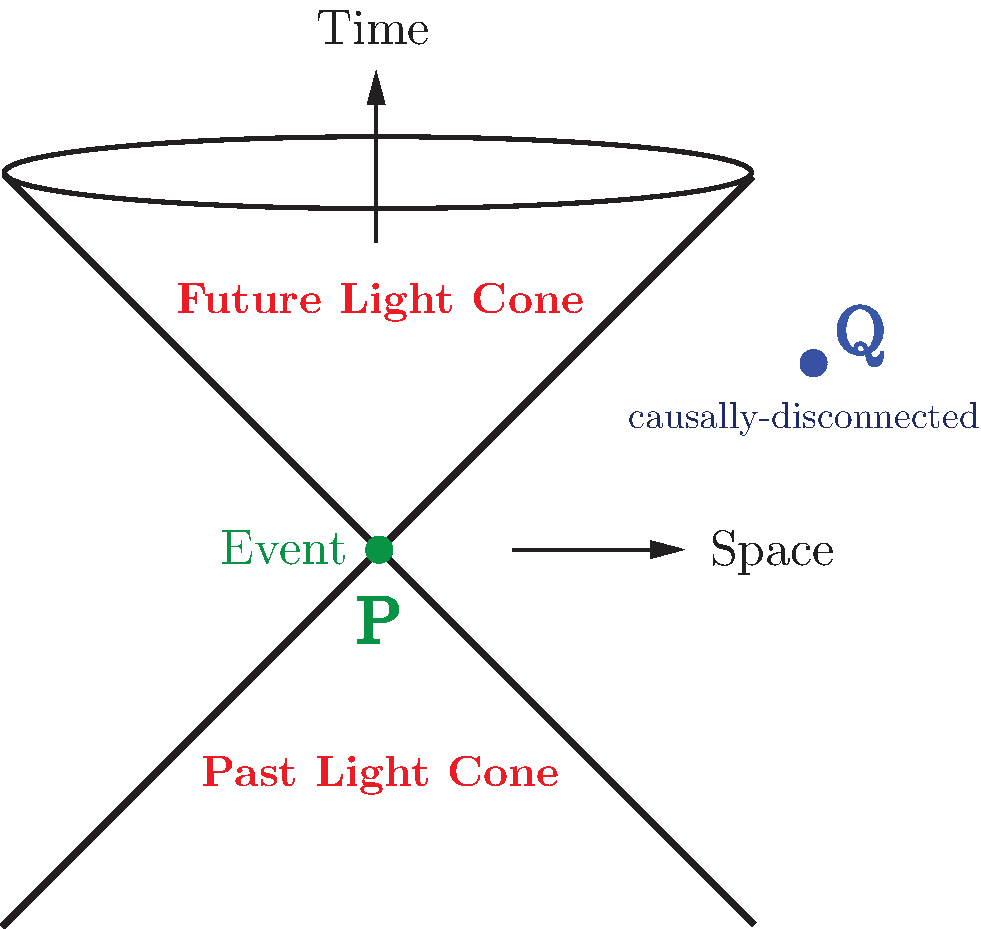
\includegraphics[width=.4\textwidth]{./lightcone}
        \caption{光円錐と因果律．光子は，{\it ヌル測地線}と呼ばれる，固有時間がゼロの世界線$\d s^2 =0$に沿って進む．
質量を持つ粒子は，{\it 時間的測地線}と呼ばれる，実数の固有時間を持つ世界線$\d s^2 > 0$に沿って進む．因果的につながっていない時空の領域は，{\it 空間的}な間隔$\d s^2 < 0$で隔てられる．時空のある点（あるいは{\it 事象}）を通るすべてのヌル測地線の集合を，{\it 光円錐}という．すべてのヌル測地線と時間的測地線からなる光円錐の内部が，その事象と因果的に関係する時空の領域を定める．}
    \label{fig:lightcone}
\end{figure}





%\vskip 6pt
%\noindent
\subsubsection*{粒子地平線}

初期時刻$t_{\rm i}$から，その後のある時刻$t$までの間に光が伝播できる最大の共動距離は，
\beq
\chi_p(\tau) = \tau - \tau_{\rm i} = \int_{t_{\rm i}}^t \frac{\d t}{a(t)}\, .
\eeq
である．これを（共動）粒子地平線と呼ぶ．初期時刻$t_{\rm i}$はしばしば，初期特異点$a(t_{\rm i} \equiv 0) \equiv 0$で定義される「宇宙の始まり」$t_{\rm i} \equiv 0$に取る．\footnote{$t_{\rm i} = 0$が$\tau_{\rm i} = 0$にも対応するかどうかは，スケール因子$a(t)$の進化に依存する．例えば，インフレーションでは$t_{\rm i}=0$は$\tau_{\rm i}=0$には{\it ならない}．}
粒子地平線の物理的な大きさは
\beq
d_p(t) = a(t) \chi_p\, .
\eeq
である．粒子地平線は，宇宙の因果構造の理解に決定的に重要であり，インフレーションの議論の基礎となる．
後に見るように，通常のビッグバン模型は過去の有限の時刻に「始まり」，過去のどの時点でも粒子地平線は有限であった．そのため，時空の領域同士が因果的に接触できた距離には限りがあった．
この特徴が「ビッグバンの謎」の核心にある．

%\vskip 6pt
%\newpage
%\noindent
\subsubsection*{事象の地平線}

事象の地平線は，ある時刻$\tau$に送られた信号が，将来にわたって観測者に届くことのない点の集合を定める．
共動座標では，これらの点は次を満たす．
\beq
\chi \ >\  \chi_e = \int_\tau^{\tau_{\rm max}} \d \tau = \tau_{\rm max} - \tau\, ,
\eeq
ここで$\tau_{\rm max}$は「時間の最後の瞬間」を表す（これは無限でも有限でもよい）．
事象の地平線の物理的な大きさは次のとおりである．
\beq
d_e(t) = a(t) \chi_e\, .
\eeq

%\vskip 6pt
%\noindent
\subsubsection*{角径距離と光度距離}

共形時間（または共動距離）は，角径距離および光度距離と簡単な関係にある．これらはそれぞれ，CMB異方性と超新星の距離を論じる際に重要である．
ここではその詳細には立ち入らないが，標準的な教科書\cite{Dodelson, Mukhanov, WeinbergCosmology}に説明がある．



\subsectionlink{力学：アインシュタイン方程式}
\label{sec:EinsteinEqns}

FRW時空のスケール因子$a(t)$の進化によって特徴付けられる宇宙の力学は，アインシュタイン方程式によって決まる．
\beq
\label{equ:Einstein}
\fbox{$\displaystyle
G_{\mu \nu} =8\pi G\, T_{\mu \nu} $}\, .
\eeq
以下ではしばしば，$8\pi G \equiv 1$となる単位系を用いる．

\subsubsection*{アインシュタイン重力}

便宜のため，ここでアインシュタイン・テンソルの定義を確認しておく．
\beq
G_{\mu \nu} \equiv R_{\mu \nu} - \frac{1}{2} g_{\mu \nu} R\, ,
\eeq
ここに現れるリッチ・テンソル$R_{\mu \nu}$とリッチ・スカラー$R$は，
\beq
R_{\mu \nu} = \Gamma^\alpha_{\ \mu \nu, \alpha} - \Gamma^\alpha_{\mu \alpha, \nu} + \Gamma^\alpha_{\ \beta \alpha} \Gamma^\beta_{\mu \nu} - \Gamma^\alpha_{\beta \nu} \Gamma^\beta_{\mu \alpha}\, , \qquad  R \equiv g^{\mu \nu} R_{\mu \nu}\, ,
\eeq
であり，
\beq
\Gamma^\mu_{\ \alpha \beta} \equiv \frac{g^{\mu \nu}}{2} \left[ g_{\alpha \nu , \beta} + g_{\beta \nu , \alpha} - g_{\alpha \beta, \nu}\right]\, .
\eeq
である．コンマは偏微分を表す．例えば，$(\dots)_{,\mu} =\frac{\partial (\dots)}{\partial x^\mu}$である．本講義では，以下もこの記法を用いる．

\subsubsection*{エネルギー，運動量，および圧力}

宇宙のエネルギー運動量テンソル$T_{\mu \nu}$を定義するため，世界線が次の時間的な4元速度ベクトルに接する観測者の集合を導入する．
\beq
u^\mu \equiv \frac{d x^\mu}{d \tau}\, ,
\eeq
ここで$\tau$は観測者の固有時間であり，$g_{\mu \nu} u^\mu u^\nu = -1$を満たす．
$u_\mu$に直交する3次元空間切片の計量として，テンソル$\gamma_{\mu \nu} \equiv g_{\mu \nu} + u_\mu u_\nu$を定義する．$\gamma_{\mu \nu}$を用い，諸量を4元速度に直交する，観測者の瞬間的な静止空間へ射影する．
すると，一般の（非完全）流体のエネルギー運動量テンソルは，次のように書ける．
\beq
T_{\mu \nu} = \rho u_\mu u_\nu + p \gamma_{\mu \nu} + 2 q_{(\mu} u_{\nu)} + \Sigma_{\mu \nu}\, ,
\eeq
ここで，$\rho = T_{\mu \nu} u^\mu u^\nu$は物質のエネルギー密度，$p = \frac{1}{3} T_{\mu \nu} \gamma^{\mu \nu}$は等方的圧力，$q_\mu = - \gamma_\mu^{\ \alpha} T_{\alpha \beta} u^\beta$はエネルギー流束ベクトル，$\Sigma_{\mu \nu} = \gamma_{\langle \mu}^{\ \alpha} \gamma_{\nu \rangle}^{\ \beta} T_{\alpha \beta}$は対称かつトレースレスな異方的応力テンソルである．\footnote{ここでは，$t_{\langle \mu \nu \rangle} = \gamma_{(\mu}^{\ \alpha} \gamma_{\nu)}^{\ \beta} t_{\alpha \beta} - \frac{1}{3} \gamma^{\alpha \beta} t_{\alpha \beta} \gamma_{\mu \nu}$および$t_{(\mu \nu)} = \frac{1}{2}(t_{\mu \nu}+t_{\nu \mu})$という記法を用いる．}
完全流体の場合，$q_\mu = \Sigma_{\mu \nu} = 0$となる4元速度が一意に存在する．すなわち，完全流体のエネルギー運動量テンソルは
\beq
T^\mu_{\ \nu} = g^{\mu \alpha} T_{\alpha \nu} = (\rho + p) \, u^\mu u_\nu - p\, \delta^\mu_\nu \, ,
%= \left( \begin{array}{cccc} \rho & 0 & 0 & 0\\ 0 & - p&0 &0 \\ 0& 0&-p&0 \\ 0&0&0& - p \end{array} \right)\, ,
\eeq
である．ここで$\rho$と$p$は流体の静止系における固有エネルギー密度と圧力であり，$u^\mu$は流体の4元速度である．
%The 4-velocity satisfies $g_{\mu \nu} u^\mu u^\nu = -1$.
流体と共動する座標系では，$u^\mu = (1,0,0,0)$と選べる．すなわち，
\beq
\label{equ:pf}
T^\mu_{\ \nu} = \left( \begin{array}{cccc} \rho & 0 & 0 & 0\\ 0 & - p&0 &0 \\ 0& 0&-p&0 \\ 0&0&0& - p \end{array} \right)\, .
\eeq
このときアインシュタイン方程式は，2本の結合した非線形常微分方程式の形になる．これらを{\it フリードマン方程式}とも呼ぶ（{\bf 問題~\ref{pro:Friedmann}}参照）．
\beq
\label{equ:Fried}
\fbox{$\displaystyle
H^2 \equiv \left(\frac{\dot a}{a}\right)^2 =  \frac{1}{3} \rho - \frac{k}{a^2}  $}\, ,
\eeq
および
\beq
\label{equ:Ray}
\fbox{$\displaystyle
\dot H + H^2 = \frac{\ddot a}{a} =  - \frac{1}{6} (\rho + 3 p) $}\, ,
\eeq
%Here we defined the Hubble parameter $H \equiv \partial_t \ln a$ as a measure of the expansion rate of the universe.
ここで，上付きのドットは物理的時間$t$に関する微分を表す．
通常の物質（すなわち強いエネルギー条件$\rho + 3 p \ge 0$を満たす物質）で満たされた膨張宇宙（すなわち$\dot a > 0$）では，式~(\ref{equ:Ray})が$\ddot a < 0$を意味することに注意しよう．これは，有限の過去に特異点$a(t\equiv 0)=0$が存在することを示す．もちろん，この結論は，一般相対性理論とフリードマン方程式が任意に高いエネルギーまで適用でき，高エネルギーで特異な形態の物質が重要にならないという仮定に依存する．
むしろ特異点は，一般相対性理論の破綻を示していると考える方が自然である．

式~(\ref{equ:Fried})と式~(\ref{equ:Ray})を組み合わせると，連続の式を得る．
\beq
\fbox{$\displaystyle
\frac{d \rho}{dt} +  3 H (\rho + p) = 0 $}\, .
\eeq
これは，次のようにも書ける．
\beq
\label{equ:conXXX}
\frac{d \ln \rho}{d \ln a} = - 3(1+w)\, ,
\eeq
ただし，状態方程式パラメータを
\beq
w \equiv \frac{p}{\rho}\, .
\eeq
と定義した．式~(\ref{equ:conXXX})を積分すると，
\beq
\rho \propto a^{-3(1+w)}\, .
\eeq
となる．これをフリードマン方程式(\ref{equ:Fried})と合わせると，スケール因子の時間発展が得られる．
\beq
a(t) \propto \left\{ \begin{array}{lc} t^{2/3(1+w)}\quad & \ w \ne -1\, , \\
e^{Ht}\quad & \ w = -1\, ,
\end{array} \right.
\eeq
すなわち，非相対論的物質（$w=0$），放射または相対論的物質（$w=\frac{1}{3}$），宇宙定数（$w=-1$）がそれぞれ支配する平坦な（$k=0$）宇宙のスケール因子は，順に$a(t)\propto t^{2/3}$，$a(t)\propto t^{1/2}$，$a(t)\propto \exp(Ht)$となる．

\begin{table}[h!]
\caption{放射，物質，または宇宙定数が支配する平坦な宇宙のFRW解．}
\label{tab:solutions}
\begin{center}
\vspace{-0.7cm}
\begin{tabular}{| l |  c | c | c | c | c|}
\hline
 & $w$ & $\rho(a) $ & $a(t)$ & $a(\tau)$ & $\tau_{\rm i}$ \\
\hline
\hline
物質優勢（MD） & 0 & $a^{-3}$ & $t^{2/3}$ & $\tau^2$ & 0\\
放射優勢（RD） & $\frac{1}{3}$ & $a^{-4}$ & $t^{1/2}$ & $\tau$ &0  \\
$\Lambda$ & $-1$ & $a^0$ & $e^{Ht}$ & $- \tau^{-1}$ & $- \infty$ \\
\hline
\end{tabular}
\end{center}
\end{table}

複数の種類の成分（バリオン，光子，ニュートリノ，ダークマター，ダークエネルギーなど）がエネルギー密度と圧力に有意に寄与する場合，$\rho$と$p$はすべての成分の和を表す．
\beq
\rho \equiv \sum_{i} \rho_{i}\, , \qquad p \equiv \sum_{i} p_{i}\, .
\eeq
各成分「${i}$」について，そのエネルギー密度の，{\it 臨界エネルギー密度}$\rho_{\rm crit} \equiv 3 H_0^2$に対する{\it 現在}の比を
\beq
\Omega_{i} \equiv {\rho_0^{i} \over \rho_{\rm crit}}\, ,
\eeq
と定義し，対応する状態方程式を
\beq
w_{i} \equiv {p_{i} \over \rho_{i}}\, .
\eeq
とする．ここで，また以下でも，添字「0」はある量を現在時刻$t_0$で評価することを表す．
スケール因子を$a_0  = a(t_0) \equiv 1$となるように規格化する．
これにより，フリードマン方程式(\ref{equ:Fried})は次のように書ける．
\beq
\label{equ:FriedX}
\left({H\over H_0}\right)^2=\sum_i\Omega_{i}
a^{-3(1+w_{i})}+\Omega_k
a^{-2},
\eeq
ここで$\Omega_k \equiv -k/a_0^2H_0^2$が曲率をパラメータ化する．
式~(\ref{equ:FriedX})を現在で評価すると，次の整合性関係を得る．
\beq
\sum_i \Omega_{i}+\Omega_k=1\, .
\eeq
第2フリードマン方程式(\ref{equ:Ray})を$t=t_0$で評価すると，
\beq
{1 \over a_0 H_0^2} {d^2 a_0 \over d t^2}=-{1\over 2}\sum_i \Omega_{i}(1+3 w_{i}).
\eeq
となる．これが，現在の加速膨張の条件を定める．



\subsectionlink{コンコーダンス模型}

 \begin{figure}[h!]
    \centering
        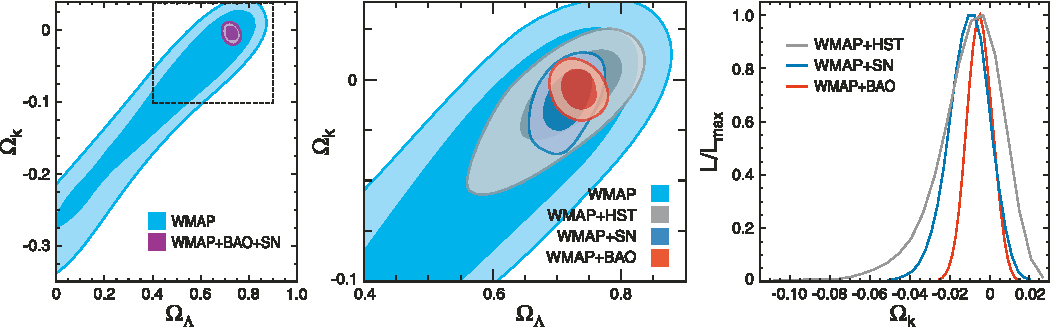
\includegraphics[width=.9\textwidth]{./KomatsuFlat}
        \caption{CMBとLSSの観測を組み合わせると，宇宙の空間的な幾何は平坦であることが示される\cite{WMAP5}．平坦性の証拠は，CMB観測だけからは得られないことに注意しよう．}
    \label{fig:flat}
\end{figure}

宇宙マイクロ波背景放射と大規模構造の観測から，宇宙は平坦であることが分かる（図~\ref{fig:flat}参照）．
\beq
\Omega_k \sim 0\, ,
\eeq
また，その構成は原子（またはバリオン「$b$」）が4\%，（冷たい）ダークマター（「$dm$」）が23\%，ダークエネルギー（$\Lambda$）が73\%である（図~\ref{fig:concord}参照）．
 \beq
 \Omega_b = 0.04\, , \ \ \Omega_{dm} = 0.23\, , \ \  \Omega_{\Lambda} = 0.72\, ,
 \eeq
ここで$w_\Lambda \approx -1$である（図~\ref{fig:concord2}参照）．
% \vspace{-1cm}
\begin{figure}[h!]
    \centering
        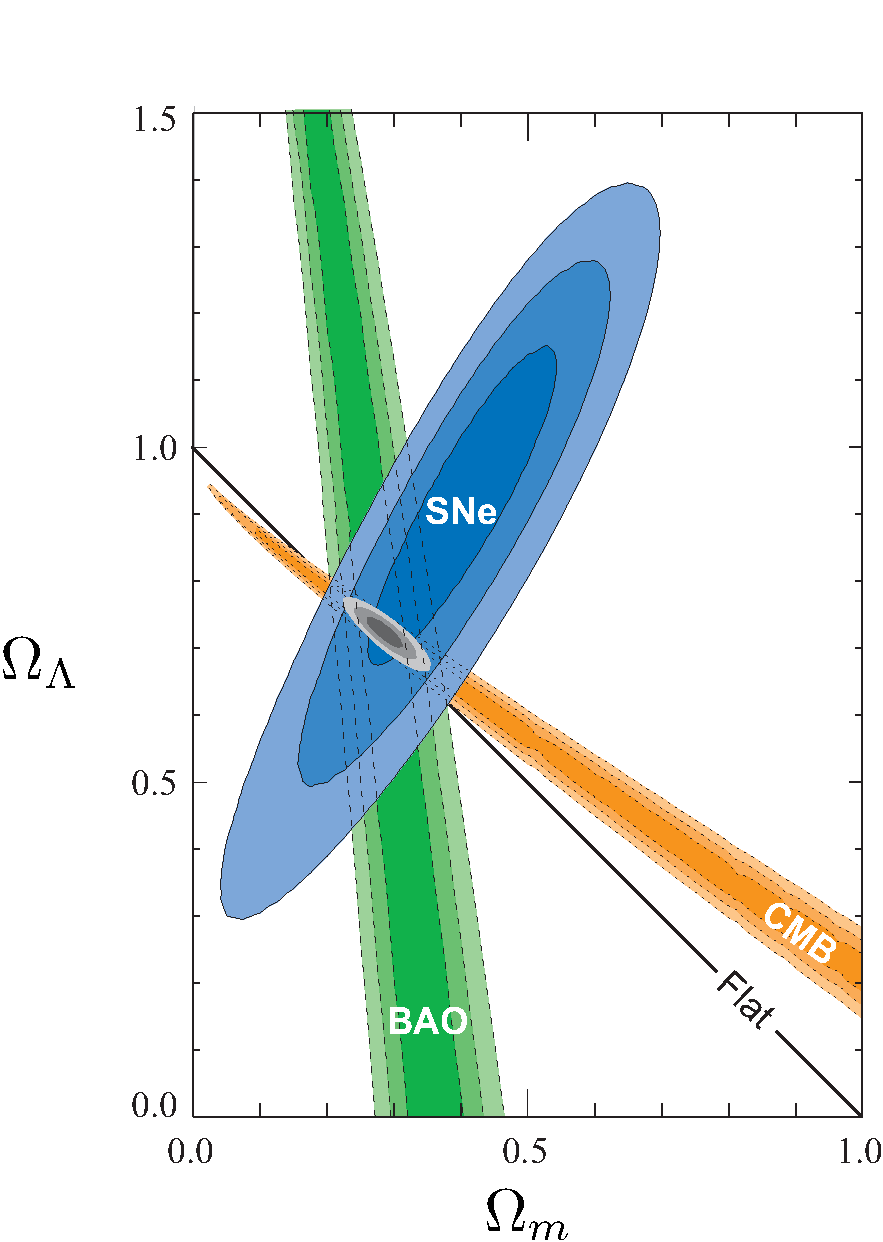
\includegraphics[width=.4\textwidth]{./DEkosowski}
        \caption{ダークエネルギーの証拠．宇宙マイクロ波背景放射（CMB），超新星（SNe），およびバリオン音響振動（BAO）の観測を組み合わせたものを示す\cite{unionsn}．}
    \label{fig:concord}
\end{figure}
 
 \begin{figure}[h!]
    \centering
        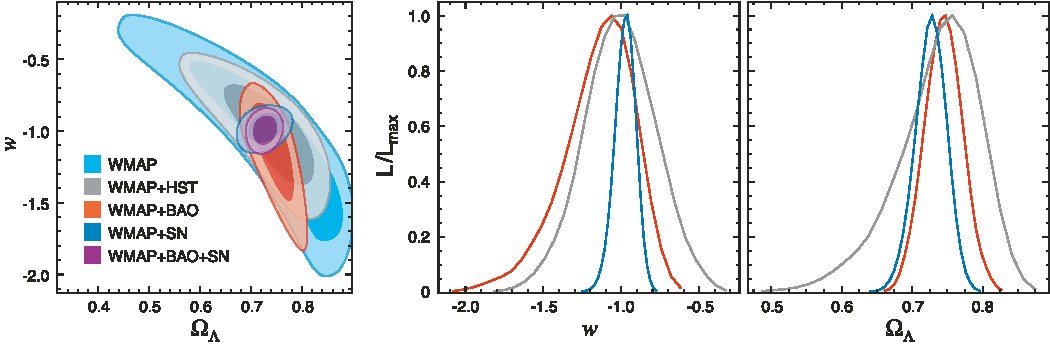
\includegraphics[width=.9\textwidth]{./KomatsuDE}
        \caption{ダークエネルギーの性質は宇宙定数に近く，$w_\Lambda \approx -1$である\cite{WMAP5}．}
    \label{fig:concord2}
\end{figure}

さらに宇宙には，断熱的でスケール不変，かつガウス的な密度揺らぎの微小なさざ波が存在することも分かっている．
%What is the physical origin of these primordial perturbations to the homogeneous universe?
本連続講義の大部分では，インフレーション中の量子揺らぎが，観測される宇宙論的摂動をどのように説明できるかを述べる．






%more than one component


%It useful to define the critical density of a flat ($k=0$) universe, $\rho_{\rm crit} = 3 H^2$.

%Define $\Omega$
\newpage
\sectionlink{ビッグバンの謎}


初期条件が物理理論の一部をなすのか，それとも別に考えるべきなのかは，いくらか哲学的な問いである．
物理学の目的は，一組の初期条件が与えられたとき，系のその後の進化を予言することにある．例えば，物体の初期位置と初期速度を定めれば，ニュートンの重力法則はその軌道を予言する．
したがって，宇宙論が宇宙の初期条件を予言すべきか，あるいは単に説明すべきかすら，決して明らかではない．
一方で，極めて特殊で微調整された初期条件からしか，私たちが見ているような宇宙が生まれず，観測される宇宙が「起こりそうもない偶然」であるとしたら，それは非常に残念なことである．

本節では，通常のビッグバン理論が，宇宙を現在の状態へ進化させるために，まさにそのような微調整された初期条件を必要とすることを説明する．
インフレーションの主要な成果の一つは，宇宙の初期条件を説明することである．
インフレーションを通じて，私たちにとって身近で大切な宇宙は，一般的な初期条件から成長した．

\subsectionlink{宇宙のコーシー問題}

宇宙の初期条件を指定するために，一定時刻の空間切片$\Sigma$を考える（ここでは，$\Sigma$の選び方のゲージ依存性は気にしない）．
3次元超曲面$\Sigma$上で，すべての物質粒子の位置と速度を定義する．
次に重力と流体力学の法則を用いて，系を時間の進む向きに発展させる．


\begin{itemize}
\item 初期の一様性

物質の空間分布を，座標${\bf x}$の関数としての密度と圧力，すなわち$\rho({\bf x})$と$p({\bf x})$で記述する．
前節では宇宙の一様性と等方性を仮定した．なぜこれはよい仮定なのだろうか．%This is particularly surprising given that i
非一様性は重力的に不安定であり，したがって時間とともに成長する．宇宙マイクロ波背景放射の観測は，過去（最終散乱時）の非一様性が，現在よりはるかに小さかったことを示している．したがって，さらに早い時刻には，これらの非一様性はもっと小さかったと予想される．
初期宇宙の滑らかさを，どう説明すればよいだろうか．

これは特に驚くべきことである．というのも，\S\ref{sec:horizon}で示すように，通常のビッグバン描像では，初期宇宙（例えば最終散乱時のCMB）は，因果的につながっていない多数の空間領域からなっていたからである．ビッグバン理論には，これらの因果的に隔てられた領域が，なぜこれほど似た物理的状況を示すのかを説明する力学的理由がない．
このため一様性の問題は，しばしば{\it 地平線問題}と呼ばれる．

\item 初期速度

宇宙のコーシー問題を完全に指定するには，初期密度分布に加えて，空間の各点における流体の速度が必要である．
後に見るように，宇宙が後期にも一様なままであることを保証するには，初期の流体速度が極めて精密な値を取らなければならない．
初期速度がわずかに小さすぎるだけで，宇宙は1秒もたたないうちに再崩壊する．
わずかに大きすぎるだけで，宇宙は急速に膨張しすぎ，たちまちほぼ空になってしまう．
この初期速度の微調整は，地平線問題と組み合わせて考えると，さらに際立つ．因果的に隔てられた空間領域にわたって，流体速度を微調整しなければならないのである．

ポテンシャルエネルギーと運動エネルギーの差が，空間領域の局所的な曲率を定めるため（{\bf 演習~\ref{ex:flatness}}参照），この初期速度の微調整は，しばしば{\it 平坦性問題}と呼ばれる．

\end{itemize}

\subsectionlink{地平線問題}
\label{sec:horizon}

前節では，{\it 共動（粒子）地平線}$\tau$を，因果的地平線，すなわち時刻$0$から時刻$t$までに光線が進める最大距離として定義した．
\beq
\fbox{$\displaystyle
\tau \equiv \int_0^t \frac{\d t'}{a(t')} = \int_0^a \frac{\d a}{Ha^2} = \int_0^a \d \ln a \left(\frac{1}{aH}\right)$}\, .
\eeq
ここでは共動地平線を，インフレーションで決定的な役割を果たす{\it 共動ハッブル半径}$(aH)^{-1}$の積分として表した．

状態方程式$w$を持つ流体が支配する宇宙では，次が成り立つ．
\beq
(aH)^{-1} = H_0^{-1} a^{\frac{1}{2}(1+3w)}\, .
\eeq 
指数が組合せ$(1+3w)$に依存することに注意しよう．
したがって，その定性的な振る舞いは，$(1+ 3 w)$が正か負かによって変わる．
%The comoving Hubble radius 
%I will show in a moment that the {\it comoving Hubble radius}, $(aH)^{-1}$, characterizes
%the fraction of comoving space in causal contact.
通常のビッグバン膨張（$w \gtrsim 0$）では，$(a H)^{-1}$は単調に{\it 増大}し，共動地平線$\tau$，すなわち{\it 因果的に接触している宇宙の割合は時間とともに増える}．
\beq
\tau \propto a^{\frac{1}{2}(1+ 3 w)}\, .
\eeq
ここでも，定性的な振る舞いは$(1+3w)$が正か負かによって変わる．
特に，放射優勢（RD）および物質優勢（MD）の宇宙について，次を得る．
\beq
\tau = \int_0^a \frac{\d a}{Ha^2} \propto
\left\{ 
\begin{array}{ll}
a \quad \quad \,\rm{RD}\\
a^{1/2} \quad \rm{MD}
\end{array} \right.  \, . 
\eeq
これは，共動地平線が時間とともに単調に増大することを意味する．したがって，現在地平線へ入ってくる共動スケールは，CMB脱結合時には地平線のはるか外にあったことになる．\footnote{揺らぎの共動波長は時間に依存しないのに対し，共動ハッブル半径は時間に依存することを思い出そう．}
%Why is the CMB uniform on large scales (of order the present horizon)?
ところがCMBがほぼ一様であることは，最終散乱の時点において，{\it 先験的には}因果的に独立しているはずの多くの領域を含むスケールにわたって，宇宙が極めて一様だったことを示している．
これはどうして可能なのだろうか．

%To be more specific,
%consider radial null geodesics in a flat FRW spacetime
%\beq
%\d s^2 = \d t^2 - a(t)^2 \d r^2 \equiv 0 \quad \quad \Rightarrow \quad \quad \d r = \pm \frac{\d t}{a(t)} \equiv \d \tau\, .
%\eeq
%We define the
%{\it comoving horizon}, $\tau$, as the causal horizon or the maximum distance a light ray can travel between time $0$ and time $t$
%\beq
%\fbox{$\displaystyle
%\tau \equiv \int_0^t \frac{\d t'}{a(t')} = \int_0^a \frac{\d a}{Ha^2} = \int_0^a \d[\ln a] \left(\frac{1}{aH}\right)$}\, .
%\eeq
%During the standard cosmological expansion the increasing comoving Hubble radius, $\frac{1}{aH}$, is therefore associated with an increasing comoving horizon\footnote{This justifies the common practice of often using the terms 'comoving Hubble radius' and 'comoving horizon' interchangeably. Although these terms should conceptually be clearly distinguished, this inaccurate use of language has become standard.}, $\tau$. In particular for radiation dominated (RD) and matter dominated (MD) universes we find
%\begin{eqnarray}
%\tau &=& \int_0^a \frac{\d a}{Ha^2} \nonumber\\
%&=& \frac{1}{H_0} \int_0^a \frac{\d a}{\Omega^{1/2}(a) a^2} \nonumber\\
%&\propto& 
%\left\{ 
%\begin{array}{ll}
%a \quad \quad \,\rm{RD}\\
%a^{1/2} \quad \rm{MD}
%\end{array} \right.  \, . 
%\end{eqnarray}
%This means that the comoving horizon grows monotonically with time (at least in an expanding universe) which implies that comoving scales entering the horizon today have been far outside the horizon at CMB decoupling.
%Why is the CMB uniform on large scales (of order the present horizon)?


\subsectionlink{平坦性問題}
\label{sec:flatness}

\begin{thm}[平坦性と運動エネルギー]
曲率パラメータ$$\Omega_k \equiv \Omega - 1= \frac{\rho-\rho_{\rm crit}}{\rho_{\rm crit}}\, , \qquad \text{ただし} \quad \rho_{\rm crit} \equiv 3 H^2\, ,$$が，空間のある領域の平均ポテンシャルエネルギーと平均運動エネルギーの差として解釈できることを示せ．
\label{ex:flatness}
\end{thm}

%{\tt Fix}

一般相対性理論の時空は力学的なものであり，宇宙の物質に応答して曲がる．それなら，なぜ宇宙は平坦なユークリッド空間でこれほどよく近似されるのだろうか．
この問題を定量化するため，フリードマン方程式を考える．
\begin{equation}
H^2 = \frac{1}{3} \rho(a) - \frac{k}{a^2}\, ,
\end{equation}
これを次のように書く．
\begin{equation}
\label{equ:omega}
\fbox{$\displaystyle
1-\Omega(a) = \frac{-k}{(aH)^2}$}\, ,
\end{equation}
ここで，
\begin{equation}
\Omega(a) \equiv \frac{\rho(a)}{\rho_{\rm crit}(a)}\, , \qquad \rho_{\rm crit}(a) \equiv 3 H(a)^2\, .
\end{equation}
である．ここでは$\Omega(a)$を時間依存する量として定義しているのに対し，前節までの$\Omega$は定数$\Omega(a_0)$であったことに注意しよう．
標準宇宙論では，共動ハッブル半径$(aH)^{-1}$は時間とともに増大するので，式~(\ref{equ:omega})から，$|\Omega-1|$も時間とともに発散しなければならない．臨界値$\Omega=1$は{\it 不安定な固定点}である．したがって，インフレーションを含まない標準ビッグバン宇宙論では，現在観測されるほぼ平坦な状態$\Omega(a_0) \sim 1$を実現するには，初期宇宙の$\Omega$を$1$の極めて近くに微調整する必要がある．
より具体的には，ビッグバン元素合成（BBN）の時期，大統一（GUT）期，およびプランク・スケールにおける平坦性からのずれは，それぞれ次の条件を満たさなければならない．
\begin{eqnarray}
|\Omega(a_{\rm BBN})-1| &\le& {\cal O}(10^{-16})\, ,\\
|\Omega(a_{\rm GUT})-1| &\le& {\cal O}(10^{-55})\, ,\\
|\Omega(a_{\rm pl})-1| &\le& {\cal O}(10^{-61})\, .
\end{eqnarray}

平坦性問題は，次の微分方程式から理解することもできる．
\begin{equation}
\label{equ:omega2}
\frac{d \Omega}{d \ln a} = (1+3w) \Omega (\Omega-1)\, .
\end{equation}
式~(\ref{equ:omega2})は，式~(\ref{equ:omega})を微分し，連続の式(\ref{equ:conXXX})を使って導かれる．これにより，強いエネルギー条件が満たされる場合には，$\Omega=1$が不安定な固定点であることが明らかになる．
\begin{equation}
\frac{d |\Omega-1|}{d \ln a} > 0 \quad \Leftrightarrow \quad 1+3w > 0\, .
\end{equation}
改めて問おう．なぜ$\Omega(a_0) \sim {\cal O}(1)$なのであって，それよりはるかに小さくも，大きくもないのだろうか．


\subsectionlink{初期条件問題について}

平坦性問題と地平線問題は，標準宇宙模型の厳密な不整合では{\it ない}ことを強調しておこう．$\Omega$の初期値が極めて1に近く，宇宙が地平線を超える距離にわたって一様に始まったと仮定すれば（ただし，構造形成を説明するのにちょうど適切な程度の非一様性を伴っていれば），宇宙は観測と一致するように，一様なまま進化し続ける．したがって，平坦性問題と地平線問題は，実際にはビッグバン模型の予言能力における深刻な欠点である．初期宇宙の驚くほどの平坦性は，標準模型から予言することができず，初期条件として仮定しなければならない．同様に，宇宙の大きなスケールでの著しい一様性も，模型によって説明も予言もされず，単に仮定しなければならない．
これらの初期条件を力学的に説明する理論は，非常に魅力的に思われる．


\sectionlink{インフレーションへの第一歩}

%\subsectionlink{Solution of the Big Bang Puzzles}

\subsectionlink{縮むハッブル球}

\S\ref{sec:horizon}と\S\ref{sec:flatness}では，標準ビッグバン宇宙論の地平線問題と平坦性問題において，共動ハッブル半径$(a H)^{-1}$が果たす根本的な役割を強調した．
どちらの問題も，通常の宇宙論では共動ハッブル半径が厳密に増大することから生じる．これは，美しいほど単純な発想によって，ビッグバンの謎をすべて解けることを示唆する．
すなわち，{\it 共動ハッブル半径の振る舞いを反転させる}，つまり{\it 極初期宇宙で共動ハッブル半径を十分に減少させる}のである．

\subsubsection{インフレーション中の共動地平線}

共動地平線の進化は，インフレーションの考え方全体にとって極めて重要なので，いくつかの重要な点を明確に述べておく価値がある．

共動地平線（＝共形時間）の定義が，共動ハッブル半径の対数積分であることを思い出そう．
\beq
\label{equ:tau}
\fbox{$\displaystyle
\tau = \int_0^a \d \ln a' \ \frac{1}{a' H(a')} $}\, .
\eeq

共動地平線$\tau$と共動ハッブル半径$(aH)^{-1}$の微妙な違いを強調しておこう\cite{Dodelson}．
\begin{quote}
粒子が$\tau$より大きな距離で隔てられていれば，それらは{\it 一度も}互いに情報をやり取りできなかった．粒子が$(aH)^{-1}$より大きな距離で隔てられていれば，それらは{\it 今}は情報をやり取りできない！ この違いは，地平線問題の解決に決定的であり，その解決は次の点に依拠する．現在の$\tau$が$(aH)^{-1}$よりはるかに大きければ，粒子は今日情報をやり取りできなくても，初期には因果的に接触していたことがありうる．式~(\ref{equ:tau})から，初期宇宙の共動ハッブル半径が現在よりもはるかに大きく，$\tau$への寄与の大部分が初期から来る場合には，これが起こりうると分かる．したがって，ハッブル半径が減少する時期が必要である．
インフレーション中は$H$がほぼ一定のまま$a$が指数関数的に増大するため，共動ハッブル半径は，まさに述べたとおり減少する．
\end{quote}

インフレーション中に共動地平線が減少することは，ビッグバンの謎を解くだけでなく，第2講で述べる宇宙論的摂動の量子的生成に必要な，鍵となる特徴でもある．量子揺らぎは地平線より小さなスケールで生成されるが，ハッブル半径がその共動波長より小さくなると，地平線の外へ出ることを説明する．物理座標では，これは超光速の膨張が摂動を因果的につながらない距離まで引き伸ばすことに対応する．それらは地平線を超える古典的な密度摂動となり，その後のビッグバンの進化で地平線へ再突入してから，重力崩壊して宇宙の大規模構造を形成する．

インフレーション中に共動地平線と共動ハッブル半径がどのように進化するかを理解したので，インフレーションがビッグバンの謎を解く仕組みの説明は，もはやほとんど自明である．

\subsubsection{平坦性問題を再考する}

平坦でない宇宙に対するフリードマン方程式(\ref{equ:omega})を思い出そう．
\begin{equation}
|1-\Omega(a)| = \frac{1}{(aH)^2}\, .
\end{equation}
共動ハッブル半径が減少すると，宇宙は平坦性から遠ざかるのでなく，{\it 平坦性へと近づいていく}．
これで平坦性問題が解決する！ インフレーション中，解$\Omega=1$はアトラクターである．

\subsubsection{地平線問題を再考する}

共動地平線が減少するということは，現在の宇宙に入ってくる大きなスケールが，インフレーション以前には地平線の内側にあったことを意味する（図2参照）．したがって，インフレーション以前の因果的な物理過程が，空間的一様性を確立した．
インフレーション期があれば，CMBの一様性は謎ではない．

%explain 60 $e$-folds from fig 2.

\begin{figure}[h]
	\centering
		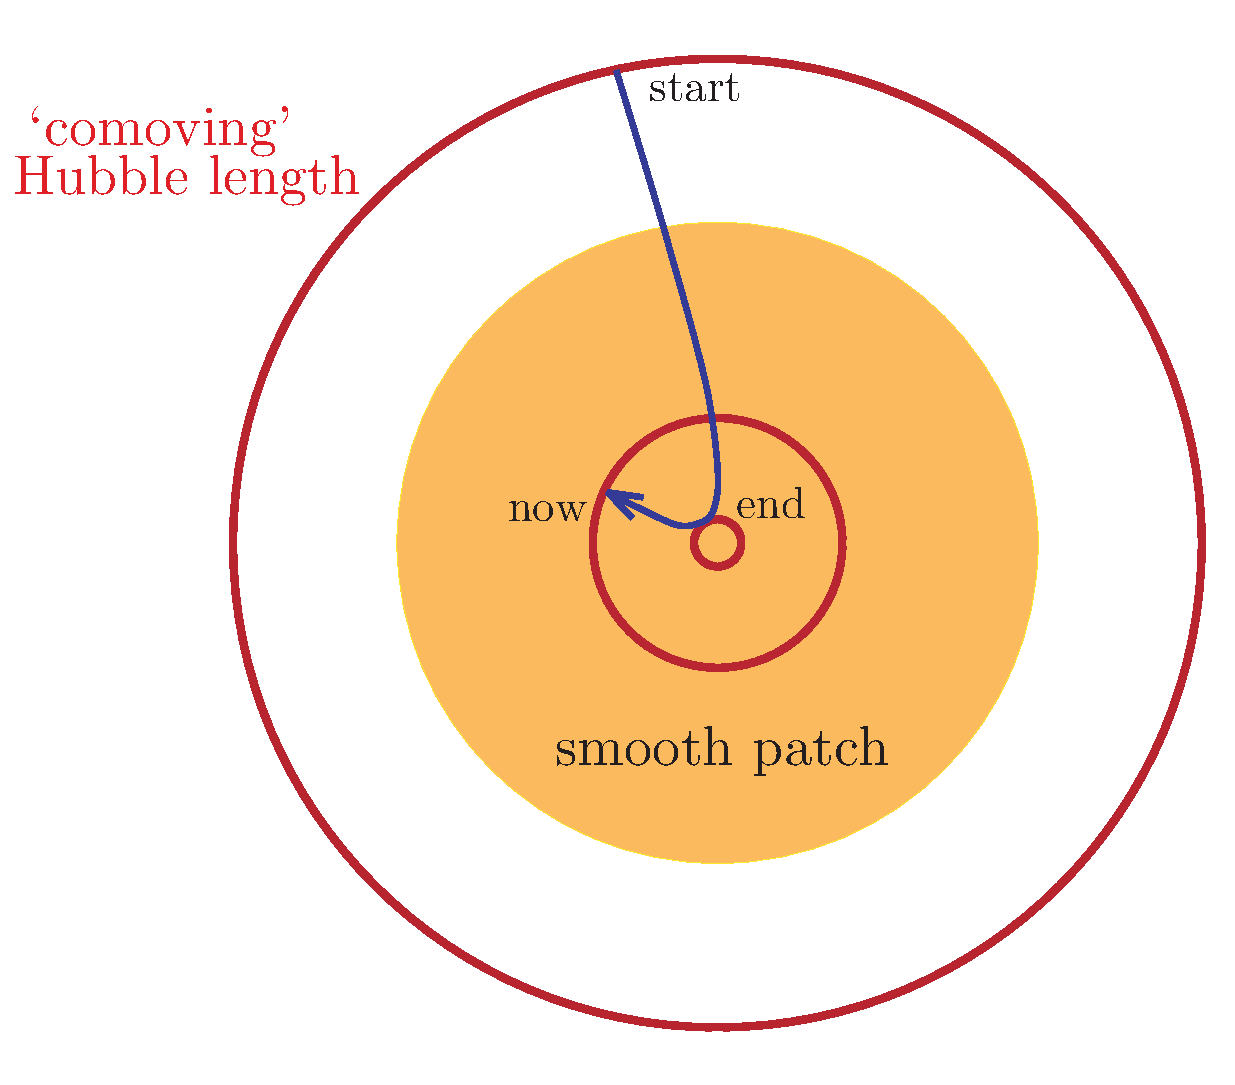
\includegraphics[width=6cm]{horizon}
		\hspace{0.5cm} 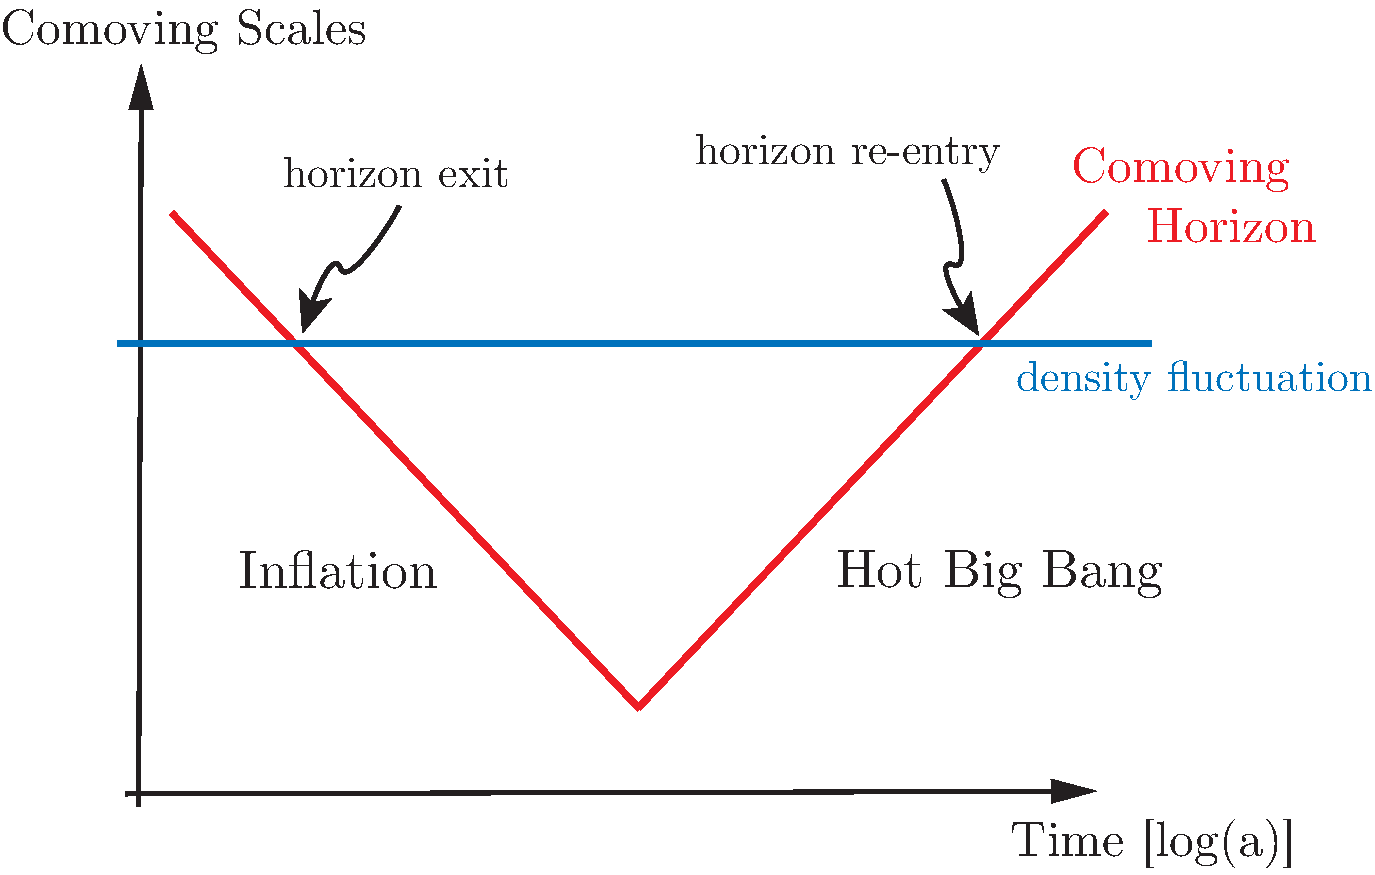
\includegraphics[width=8cm]{Scales}
	\label{fig:horizon}
\caption{{\it 左：}インフレーション宇宙における共動ハッブル半径$(aH)^{-1}$の進化．
	%[Figure adapted from Liddle and Lyth \cite{LiddleLyth}.] 
共動ハッブル球はインフレーション中に縮み，インフレーション後に膨張する．
したがってインフレーションは，地平線より小さな滑らかな領域を「拡大して見る」機構である．
{\it 右：}地平線問題の解決．今日の宇宙論的観測に関係するすべてのスケールは，$a\sim 10^{-5}$まではハッブル半径より大きかった．しかし，十分に早い時刻には，これらのスケールはハッブル半径より小さく，したがって因果的につながっていた．同様に，宇宙論的に関心のあるスケールは，比較的最近になってハッブル半径の内側に再び入ってきた．}
\end{figure}


\subsectionlink{インフレーションの条件}

フリードマン方程式を通じて，共動ハッブル半径の縮小は，宇宙の加速および圧力に関係付けられる．
\beq
\fbox{$\displaystyle
\frac{d}{d t} \left(\frac{H^{-1}}{a}\right) < 0 \quad \Rightarrow \quad {d^2 a \over d t^2} >0 \quad \Rightarrow \quad \rho+3p <0 $}\, .
\eeq
したがって，インフレーションの三つの同値な条件は次のとおりである．
\begin{itemize}
\item {\bf 共動地平線の減少}

縮小するハッブル球は，次の条件で定義される．
\beq
\frac{d}{d t} \left(\frac{1}{aH}\right) < 0\, .
\eeq
これをインフレーションの基本的な定義として用いたのは，平坦性問題と地平線問題に最も直接に関係し，揺らぎを生成する機構の鍵となるからである．

\item {\bf 加速膨張}

関係式
\beq
\frac{d}{d t} (a H)^{-1} = \frac{- \ddot a}{(a H)^2}\, ,
\eeq
から，共動ハッブル半径の縮小が加速膨張を意味することが直ちに分かる．
\beq
{d^2 a \over d t^2 } >0\, . 
\eeq
これが，インフレーションがしばしば加速膨張期と定義される理由である．
もちろんスケール因子の時間に関する2階微分は，ハッブル・パラメータ$H$の時間に関する1階微分に関係付けられる．
\beq
\frac{\ddot a}{a} = H^2 (1-\varepsilon)\, , \qquad \text{ただし} \quad \varepsilon \equiv  - \frac{\dot H}{H^2}\, .
\eeq
したがって加速は，次の条件に対応する．
\beq
\label{equ:eps}
\fbox{$\displaystyle
\varepsilon = - \frac{\dot H}{H^2} = - \frac{d \ln H}{d N}< 1 $}
\eeq
ここでは$\d N = H \d t = \d \ln a$と定義した．これは，インフレーションによる膨張の$e$-fold数$N$を測る．
したがって式~(\ref{equ:eps})は，1 $e$-fold当たりのハッブル・パラメータの相対変化が小さいことを意味する．

 
\item {\bf 負の圧力}

どのようなエネルギー運動量が，加速を引き起こせるだろうか．
式~(\ref{equ:Ray})を参照すると，$\ddot a > 0$には次が必要であると分かる．
\beq
p < - \frac{1}{3} \rho\, ,
\eeq
すなわち，負の圧力，あるいは強いエネルギー条件（SEC）の破れが必要である．
これが物理理論でどのように実現されるかは，\S\ref{sec:SR}で説明する．
SECは決して絶対的なものではなく，容易に破られうることが分かるだろう．
\end{itemize}


\subsectionlink{インフレーションの共形図}

\begin{figure}
	\centering
		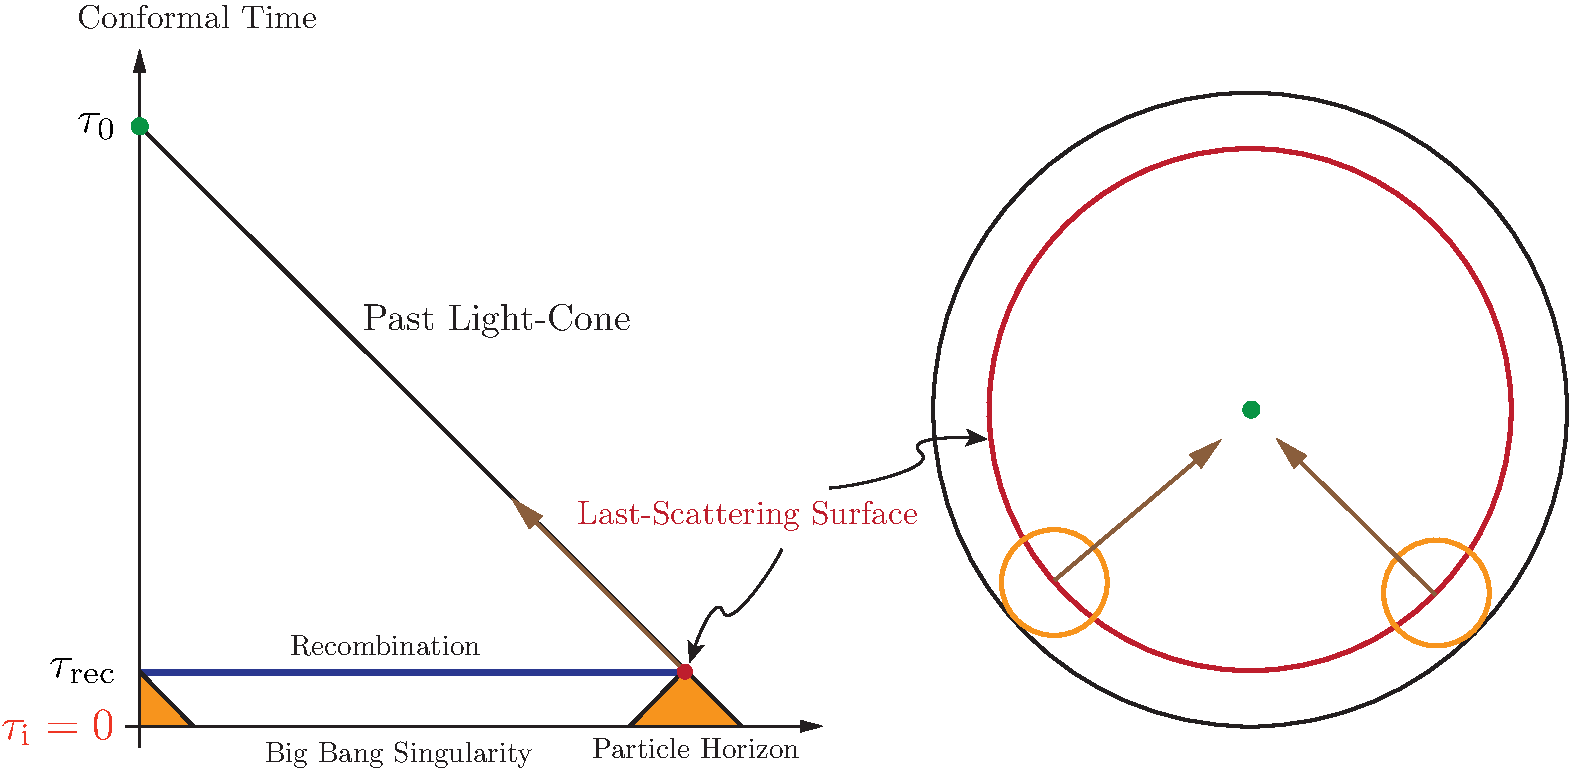
\includegraphics[width=0.98\textwidth]{FRWHorizon}
\caption{ビッグバン宇宙論の共形図．最終散乱（再結合）時のCMBは，因果的につながっていない$10^5$個の領域からなる！}
	\label{fig:Conformal1b}
\end{figure}
\begin{figure}
	\centering
		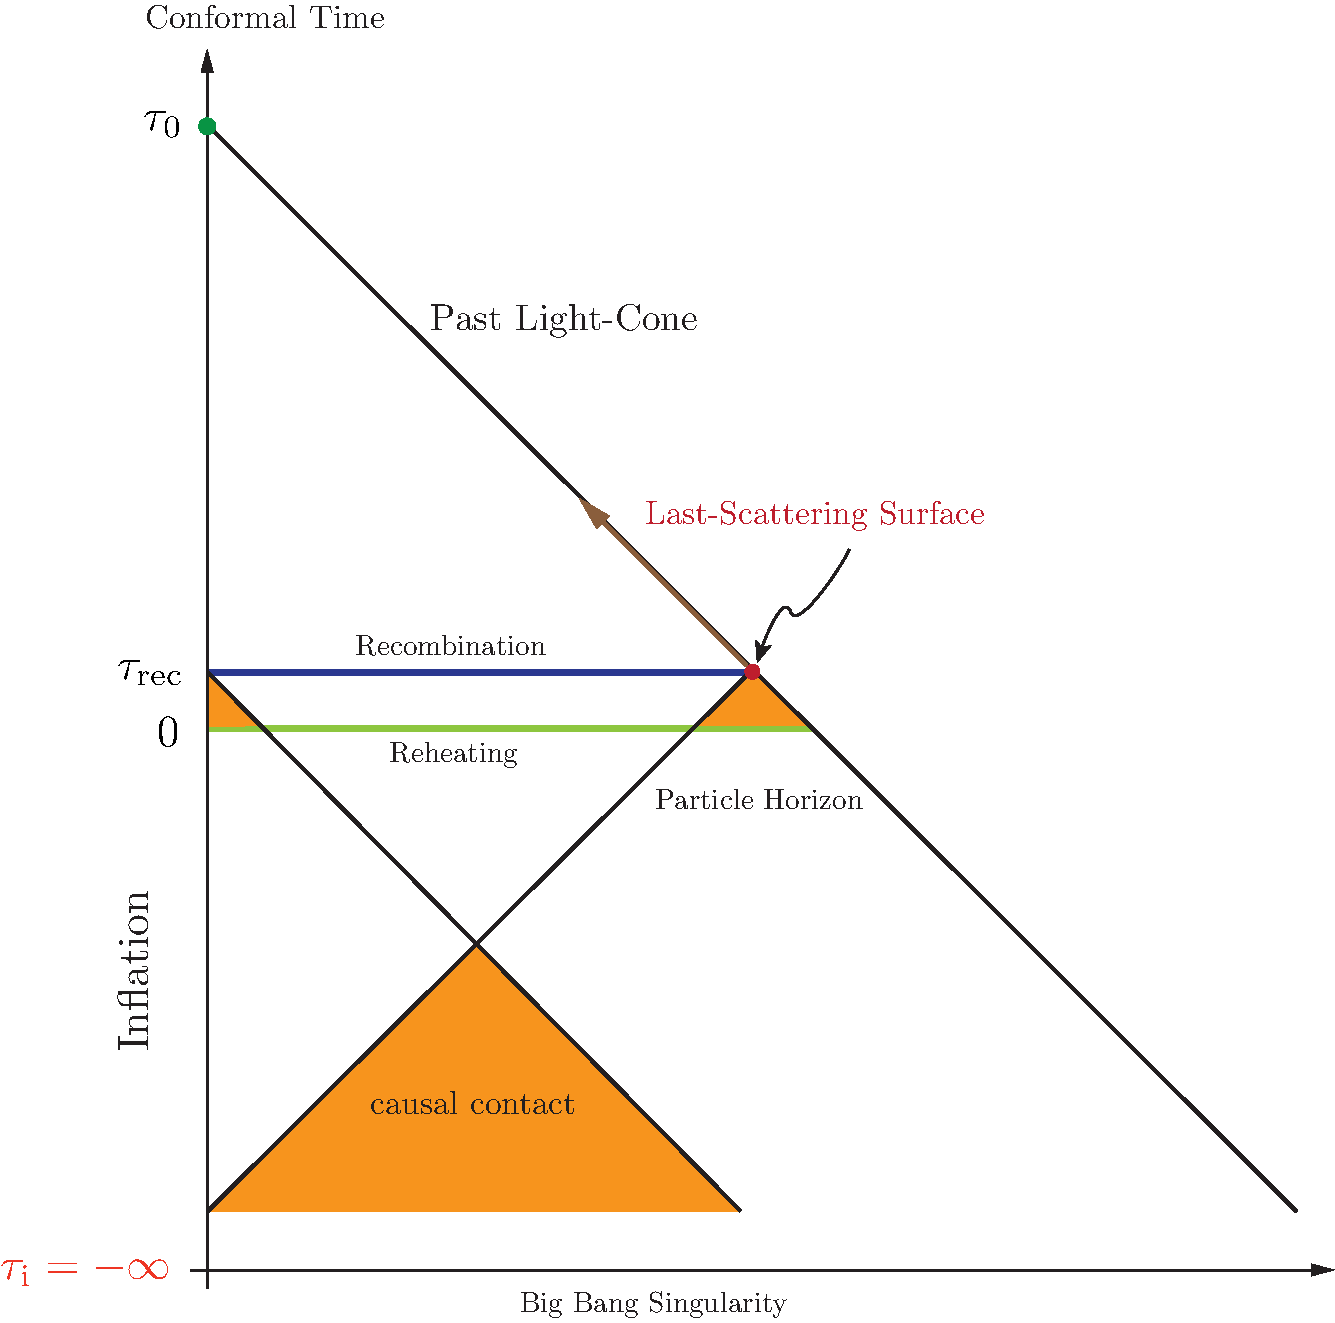
\includegraphics[width=0.95\textwidth]{InflationHorizon}
\caption{インフレーション宇宙論の共形図．インフレーションは共形時間を負の値へと拡張する！ インフレーションの終了は，$\tau = 0$に「見かけの」ビッグバンを作り出す．しかし$\tau =0$に特異点はなく，インフレーションが少なくとも60 $e$-fold続けば，光円錐はより早い時刻で交わる．}
		\label{fig:Conformal2}
\end{figure}

インフレーションを可視化するうえで，共形時空図は実に示唆に富む方法である．
\S\ref{sec:FRW}から，共形時間$\d \tau =\d t/a(t)$で表した平坦なFRW計量を思い出そう．
\beq
\d s^2 =a^2(\tau) \left[- \d \tau^2 + \d {\bf x}^2 \right]\, .
\eeq
また共形座標では，ヌル測地線（$\d s^2$\,=\,$0$）は常に$45^\circ$の角度をなし，$\d \tau = \pm \sqrt{\d {\bf x}^2} \equiv \pm \d r$であることも思い出そう．光は時空の因果構造を決めるので，これはインフレーション宇宙論における地平線を調べるのに適した方法を与える．%and thermal equilibrium

物質優勢期または放射優勢期には，スケール因子は次のように進化する．
\beq
a(\tau) \propto
\left\{ 
\begin{array}{ll}
\tau \quad \,\, \text{RD}\\
\tau^2 \quad \text{MD}
\end{array} \right. \, .
\eeq 
宇宙が常に物質か放射に支配されていた場合に限り，これは$\tau_{\rm i} = 0$に{\it ビッグバン特異点}が存在することを意味する．
\beq
a(\tau_{\rm i} \equiv 0) = 0\, .
\eeq
標準ビッグバン宇宙論に対応する共形図を，図~\ref{fig:Conformal1b}に示す．地平線問題は明らかである．共形図の各時空点には，その因果的な過去を定める過去光円錐が対応する．ある$\tau = \text{一定}$の面上の2点は，その過去光円錐がビッグバン$\tau_{\rm i} = 0$で交われば，因果的に接触している．これは，最終散乱面（$\tau_{\rm CMB}$）が，熱平衡になりえない，因果的につながっていない多数の領域からなっていたことを意味する．したがって，大きなスケールにおけるCMBの一様性は深刻な謎となる．

インフレーション中（$H \approx {\rm const.}$），スケール因子は
\beq
\label{equ:dS}
a(\tau) = -\frac{1}{H \tau}\, ,
\eeq
となり，特異点$a=0$は無限の過去$\tau_{\rm i} \to -\infty$へ押しやられる．
スケール因子(\ref{equ:dS})は，$\tau = 0$で無限大になる！ これは$H = \text{const.}$であるド・ジッター空間を仮定したためであり，インフレーションが永遠に続き，$\tau = 0$が無限の未来$t \to +\infty$に対応することを意味する．実際にはインフレーションはある有限の時刻に終わり，近似(\ref{equ:dS})は初期には有効であっても，インフレーションの終わり近くで成り立たなくなる．したがって面$\tau =0$はビッグバンではなく，インフレーションの終わりである．初期特異点は，共形時間で任意に遠い過去$\tau \ll 0$に押し戻され，光円錐は見かけのビッグバンを通り抜けて延びることができるため，一見つながっていないように見える点も因果的に接触する．
言い換えれば，インフレーションによって「再結合以前には，私たちが考えていたより多くの（共形）時間があった」のである．
これを図~\ref{fig:Conformal2}の共形図にまとめている．



\sectionlink{インフレーションの物理}
\label{sec:SR:source-duplicate-1}

インフレーションは，非常になじみのない物理現象である．
1秒にも満たない間に，宇宙は加速しながら指数関数的に大きくなった．
アインシュタイン重力では，これは負の圧力を持つ源，あるいは同じことだが，ほぼ一定のエネルギー{\rm 密度}を必要とする．
本節では，これが実現される物理的条件を述べる．


\subsectionlink{スカラー場の力学}

\begin{figure}[htbp]
    \centering
        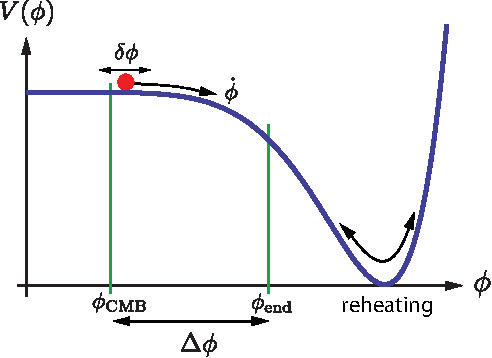
\includegraphics[width=0.45\textwidth]{SmallField}
   \caption{\small インフラトン・ポテンシャルの例．場のポテンシャルエネルギー$V(\phi)$が運動エネルギー$\frac{1}{2} \dot \phi^2$を支配すると，加速が生じる．
運動エネルギーが増大してポテンシャルエネルギーと同程度，$\frac{1}{2} \dot \phi^2 \approx V$になると，$\phi_{\rm end}$でインフレーションは終わる．
CMBの揺らぎは，インフレーション終了の約60 $e$-fold前に，量子揺らぎ$\delta \phi$によって作られる．再加熱の際に，インフラトンのエネルギー密度は放射へと変換される．}
    \label{fig:small}
\end{figure}

最も単純なインフレーション模型は，{\it インフラトン}と呼ばれる単一のスカラー場$\phi$を含む．
ここでは場$\phi$の物理的な正体を特定せず，インフレーションのエネルギー密度の時間発展をパラメータ化する，秩序変数（または時計）として用いるだけにする．
重力に（最小）結合したスカラー場の力学は，次の作用に従う．
\beq
\label{equ:phiaction}
\fbox{$\displaystyle
S = \int \d^4 x \sqrt{-g} \left[\frac{1}{2} R + {1\over 2} g^{\mu \nu} \partial_\mu\phi \, \partial_\nu\phi
-V(\phi) \right]$} = S_{\rm EH} + S_\phi\, .
\eeq
作用(\ref{equ:phiaction})は，重力のアインシュタイン・ヒルベルト作用$S_{\rm EH}$と，正準運動項を持つスカラー場の作用$S_\phi$の和である．
ポテンシャル$V(\phi)$は，スカラー場の自己相互作用を記述する．
スカラー場のエネルギー運動量テンソルは，%given by
\beq
T_{\mu\nu}^{(\phi)} \equiv -\frac{2}{\sqrt{-g}} \frac{\delta S_\phi}{\delta g^{\mu \nu}} = \partial_\mu\phi\partial_\nu\phi-g_{\mu\nu}
\left({1\over 2}\partial^\sigma\phi\partial_\sigma\phi
+V(\phi)\right).
\label{Tscalarfield}
\eeq
である．場の運動方程式は
\beq
\frac{\delta S_\phi}{\delta \phi} = \frac{1}{\sqrt{-g}} \partial_\mu (\sqrt{-g} \partial^\mu \phi) + V_{, \phi}= 0\, ,
\eeq
であり，$V_{, \phi} = \frac{dV}{d\phi}$である．
$g_{\mu \nu}$にFRW計量(\ref{equ:FRW})を仮定し，一様な場$\phi(t, {\bf x}) \equiv \phi(t)$の場合に限ると，スカラー場のエネルギー運動量テンソルは，次の密度と圧力を持つ完全流体(\ref{equ:pf})の形になる．
\begin{eqnarray}
\rho_\phi &=& {1\over 2}\dot\phi^2+V(\phi)\, , \\
p_\phi &=& {1\over 2}\dot\phi^2-V(\phi)\, .
\end{eqnarray}
この結果得られる状態方程式
\beq
\fbox{$\displaystyle
w_\phi  \equiv \frac{p_\phi}{\rho_\phi} = \frac{\frac{1}{2} \dot{\phi}^2 -V}{\frac{1}{2} \dot{\phi}^2 +V}$}\, ,
\eeq
から，ポテンシャルエネルギー$V$が運動エネルギー$\frac{1}{2} \dot{\phi}^2$を支配すると，スカラー場は負の圧力（$w_\phi< 0$）と加速膨張（$w_\phi<-1/3$）をもたらしうることが分かる．
（一様な）スカラー場とFRW幾何の力学は，次の式で決まる．
\beq
\ddot\phi+3H\dot \phi+V_{,\phi}=0 \qquad \text{および} \qquad H^2={1\over 3}\left({1\over 2}\dot\phi^2+V(\phi)\right)\, .
\eeq
ポテンシャルの値が大きいと，場には$H \dot \phi$の項から大きなハッブル摩擦が働く．

\subsectionlink{スローロール・インフレーション}
\label{sec:SR}

一様なスカラー場が支配する宇宙の加速度方程式は，次のように書ける．
\beq
\frac{\ddot a}{a} = - \frac{1}{6} (\rho_\phi + 3 p_\phi) = H^2 (1-\varepsilon)\, ,
\eeq
ここで，
\beq
\varepsilon \equiv \frac{3}{2} (w_\phi + 1) = \frac{1}{2} \frac{\dot \phi^2}{H^2}\, .
\eeq
である．いわゆる{\it スローロール・パラメータ}$\varepsilon$は，ハッブル・パラメータの進化に関係付けられる．
\beq
\fbox{$\displaystyle
\varepsilon = - \frac{\dot H}{H^2}$} = - \frac{d \ln H}{d N}\, ,
\eeq
ここで$\d N = H \d t$である．
$\varepsilon < 1$なら加速膨張が生じる．ド・ジッター極限$p_\phi \to - \rho_\phi$は，$\varepsilon \to 0$に対応する．
この場合，ポテンシャルエネルギーが運動エネルギーを支配する．
\beq
\dot \phi^2 \ll V(\phi)\, .
\eeq
%Inflation occurs if the field is evolving slow enough that the potential energy dominates the kinetic energy, and the second time derivative of $\phi$ is small enough to allow this slow-roll condition to be maintained for a sufficient period. Thus, inflation requires
%\begin{eqnarray}
%\dot{\phi}^2 &\ll& V(\phi)\, \\
%|\ddot{\phi}| &\ll& |3H \dot{\phi}|, |V_{,\phi}|\, .
%\end{eqnarray}
加速膨張が十分に長い時間続くためには，$\phi$の時間に関する2階微分が十分に小さくなければならない．
\beq
|\ddot{\phi}| \ \ll \ |3H \dot{\phi}|\, , \, |V_{,\phi}|\, .
\eeq
これは，第2のスローロール・パラメータが小さいことを必要とする．
\beq
\eta = - \frac{\ddot \phi}{H \dot \phi} = \varepsilon - \frac{1}{2 \varepsilon} \frac{d \varepsilon}{d N}\, ,
\eeq
ここで$|\eta| < 1$は，1 $e$-fold当たりの$\varepsilon$の相対変化が小さいことを保証する．
%Satisfying these conditions requires the smallness of two dimensionless quantities known as {\it slow-roll parameters}
スローロール条件$\varepsilon, |\eta| < 1$は，インフレーション・ポテンシャルの形に対する条件として表すこともできる．
\begin{equation}
\fbox{$\displaystyle \epsilon_{\rm v}(\phi) \equiv \frac{M_{\rm pl}^2}{2} \left(\frac{V_{,\phi}}{V}\right)^2 $}\, ,
\end{equation}
および
\begin{equation}
\fbox{$\displaystyle
\eta_{\rm v}(\phi) \equiv M_{\rm pl}^2 \frac{V_{,\phi\phi}}{V} $}\, .
\end{equation}
ここでは$\epsilon_{\rm v}$と$\eta_{\rm v}$が無次元であることを明示するため，一時的にプランク質量を再導入した．
以下では再び$M_{\rm pl}$を1と置く．
スローロール領域
\beq
\label{equ:SR}
\epsilon_{\rm v}, |\eta_{\rm v}| \ll 1\, ,
\eeq
では，背景の進化は
\begin{eqnarray}
H^2 &\approx& {1\over 3} V(\phi) \approx \text{const.}\, , \label{equ:SRH}\\
\dot{\phi} &\approx& -\frac{V_{,\phi}}{3H} \label{equ:SRphi}\, ,
\end{eqnarray}
となり，時空は近似的に{\it ド・ジッター}時空となる．
\begin{equation}
a(t) \sim e^{Ht}\, . % , \quad  {\rm where} \quad H \approx \text{const}\, .
\end{equation}
パラメータ$\epsilon_{\rm v}$と$\eta_{\rm v}$は，{\it ハッブル・スローロール・パラメータ}$\varepsilon$および$\eta$と区別するため，{\it ポテンシャル・スローロール・パラメータ}と呼ばれる．
スローロール近似では，ハッブルおよびポテンシャルのスローロール・パラメータは次のように関係する（付録~\ref{sec:HSR}参照）．
\beq
\varepsilon \approx \epsilon_{\rm v} \, , \qquad \eta \approx \eta_{\rm v} - \epsilon_{\rm v}\, .
\eeq
%To understand the relation between the slow-roll condition (\ref{equ:SR}) and inflation it is helpful to convince yourself that the following is true
%\beq
%\label{equ:SR2}
%\frac{\ddot{a}}{a} = H^2 \left(1+\frac{\dot H}{H^2}\right) \approx H^2 (1-\epsilon_{\rm v})\, .
%\eeq
%Consequently, if the slow-roll approximation is valid ($\epsilon_{\rm v} \ll 1$), then inflation is guaranteed. However, this condition is sufficient but not necessary since the validity of the slow-roll approximation was required to establish the second equality in (\ref{equ:SR2}).

スローロール条件が破れると，インフレーションは終了する．%(\ref{equ:SR})
%\footnote{This can be made exact by the use of Hubble slow-roll parameters instead of the potential slow-roll parameters we introduced here (see Appendix B).}
\beq
\varepsilon(\phi_{\rm end}) \equiv 1\, , \qquad \epsilon_{\rm v}(\phi_{\rm end}) \approx 1\, .
\eeq
インフレーションが終了するまでの$e$-fold数は，
\begin{eqnarray}
N(\phi) &\equiv& \ln \frac{a_{\rm end}}{a} \nonumber\\
&=&\int_t^{t_{\rm end}} H \d t = \int_\phi^{\phi_{\rm end}} \frac{H}{\dot \phi} \d \phi 
\approx \int_{\phi_{\rm end}}^\phi \frac{V}{V_{,\phi}} \d \phi \, , \label{equ:Nphi}
\end{eqnarray}
である．ここでは，スローロールの結果(\ref{equ:SRH})と(\ref{equ:SRphi})を用いた．
結果(\ref{equ:Nphi})は，次のようにも書ける．
\beq
\fbox{$\displaystyle
N(\phi) = \int_{\phi_{\rm end}}^\phi \frac{\d \phi}{\sqrt{2\varepsilon}}  \approx \int_{\phi_{\rm end}}^\phi \frac{\d \phi}{\sqrt{2\epsilon_{\rm v}}} $}\, .
\eeq
地平線問題と平坦性問題を解くには，インフレーションの総$e$-fold数が約60を超える必要がある．
\beq
N_{\rm tot} \equiv \ln \frac{a_{\rm end}}{a_{\rm start}} \gtrsim 60\, .
\eeq
正確な値は，インフレーションのエネルギースケールと，インフレーション後の再加熱の詳細に依存する．
CMBで観測される揺らぎは，インフレーションの終了より$N_{\rm cmb} \approx 40-60$ $e$-fold前に作られる（正確な値は，やはり再加熱とインフレーション後の宇宙の熱史の詳細に依存する）．以下の積分制約から，それに対応する場の値$\phi_{\rm cmb}$が得られる．
\beq
 \int_{\phi_{\rm end}}^{\phi_{\rm cmb}} \frac{\d \phi}{\sqrt{2\epsilon_{\rm v}}} = N_{\rm cmb} \approx 40 -60\, .
\eeq


\subsectionlink{具体例：$m^2 \phi^2$インフレーション}

一例として，おそらく最も単純なインフレーション模型，すなわち質量項によって駆動される単一場インフレーションのスローロール解析を行おう．
\beq
V(\phi) = \frac{1}{2} m^2 \phi^2\, .
\eeq
スローロール・パラメータは，
\beq
\epsilon_{\rm v}(\phi) = \eta_{\rm v}(\phi) = 2 \left( \frac{M_{\rm pl}}{\phi}\right)^2\, .
\eeq
である．スローロール条件$\epsilon_{\rm v}, |\eta_{\rm v}| < 1$を満たすには，インフラトンについて，プランク質量を超える場の値を考えなければならない．
\beq
\phi > \sqrt{2} M_{\rm pl} \equiv \phi_{\rm end}\, .
\eeq
インフラトンの場の値と，インフレーション終了までの$e$-fold数の関係は，
\beq
N(\phi) = \frac{\phi^2}{4 M_{\rm pl}^2} - \frac{1}{2}\, .
\eeq
である．CMBで観測される揺らぎは，次の場の値で生成される．
\beq
\phi_{\rm cmb} = 2 \sqrt{N_{\rm cmb}} \, M_{\rm pl} \sim 15 M_{\rm pl}\, .
\eeq
次の講義では，$m^2 \phi^2$インフレーションが生成する揺らぎのスペクトルを計算する際に，この例に戻る．

\begin{thm}[$m^2 \phi^2$インフレーション]
$m^2 \phi^2$インフレーションについて，上記のスローロールの結果を確かめよ．
\label{ex:chaotic}
\end{thm}

\subsectionlink{再加熱}

インフレーションが終了すると，スカラー場はポテンシャルの極小点のまわりで振動し始める．
このコヒーレントな振動の時期には，スカラー場は圧力のない物質のように振る舞う．
\beq
\label{equ:coherent}
\frac{d \bar \rho_\phi}{dt} + 3H \bar \rho_\phi = 0\, .
\eeq

\begin{thm}[スカラー場のコヒーレントな振動]
$\phi$の運動方程式から，式~(\ref{equ:coherent})を確かめよ．
\label{ex:coherent}
\end{thm}

インフラトン場と他の粒子との結合によって，インフラトンのエネルギーが崩壊する．
\beq
\frac{d \bar \rho_\phi}{dt} +(3H+ \Gamma_\phi) \bar \rho_\phi = 0\, .
\eeq
結合パラメータ$\Gamma_\phi$は，複雑で模型に依存した物理過程によって決まるが，ここではそれらを概説する時間はない．
最終的にインフレーションのエネルギー密度は標準模型の自由度へと変換され，熱いビッグバンが始まる．
%a few words on preheating

再加熱は豊かで複雑な主題であり，本講義では十分に扱うことができない．
詳しく知りたい読者には，Bassettらの総説\cite{BassettReview}を勧める．


%Give expression for number of e-folds.


\subsectionlink{インフレーションの模型}

インフレーションの根本的な微視的起源は，今も謎である．インフラトンとは何か，インフレーション・ポテンシャルはどのような形か，なぜ宇宙は高エネルギー状態から始まったのか，といった基本的な問いは未解決のままである．インフレーションの物理を説明するという課題は，非常に難しい．インフレーションは，地上の粒子加速器では到底到達できない，巨大なエネルギースケール（$\sim 10^{15}$ GeVにも達するかもしれない）で起こったと考えられている．したがって，インフレーション期を記述するには，既知の物理法則を大幅に外挿する必要があり，最近までは，インフレーションの力学を現象論的にパラメータ化することしかできなかった．\footnote{最近では，インフレーションの系統的な有効場の理論による記述\cite{PaoloEFT, WeinbergEFT}と，弦理論からのトップダウンによるインフレーション・ポテンシャルの導出\cite{BMReview}の両方で進展があった．}このアプローチでは，適切なインフレーション・ポテンシャル関数$V(\phi)$を仮定し（よく使われる二つの例については図~\ref{fig:small}と図~\ref{fig:large}を参照），そこから実験的予言を計算する．次の講義で見るように，原始揺らぎのスペクトルの詳細は，インフラトン・ポテンシャルの正確な形に依存する．


\subsubsection{単一場スローロール・インフレーション}

インフレーション模型を定義することは，インフラトンの作用（ポテンシャル項と運動項）およびその重力との結合を指定することに等しい．
これまでは，最も単純な模型，すなわち次の作用で特徴付けられる単一場スローロール・インフレーションの言葉で議論してきた．
\beq
\label{equ:simple}
S = \int \d^4 x \sqrt{-g} \left[\frac{1}{2} R + {1\over 2} g^{\mu \nu} \partial_\mu\phi \, \partial_\nu\phi
-V(\phi) \right]\, .
\eeq
CMBの揺らぎが生成された$\phi_{\rm cmb}$の時点（{\bf 第2講}参照）から，$\phi_{\rm end}$でインフレーションが終わるまでのインフラトン場の力学は，インフレーション・ポテンシャル$V(\phi)$の形によって決まる．
$V(\phi)$のさまざまな可能性は，インフラトン場が移動する距離$\Delta \phi \equiv \phi_{\rm cmb} -\phi_{\rm end}$が，プランク単位で測って大きいか小さいかによって分類すると便利である．

\begin{figure}[htbp]
    \centering
        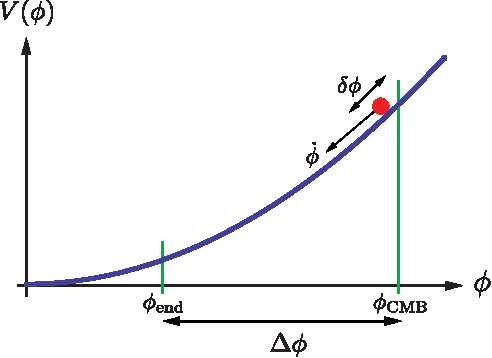
\includegraphics[width=0.4\textwidth]{LargeField}
   \caption{\small 大場インフレーション．重要な一群のインフレーション模型では，インフレーションの力学はポテンシャルの単一の単項式項$V(\phi) \propto \phi^p$によって駆動される．これらの模型では，インフラトン場はインフレーション中にプランク質量を超える範囲$\Delta \phi > M_{\rm pl}$を動き，量子力学的揺らぎによって大振幅の重力波が生成される（{\bf 第2講}参照）．}
    \label{fig:large}
\end{figure}

\begin{enumerate}
\item {\it 小場インフレーション}

小場模型では，場は小さな（プランク質量未満の）距離$\Delta \phi < M_{\rm pl}$を動く．
これは将来の観測に関係する．小場模型は，インフレーション中に生成される重力波の振幅が小さすぎて検出できないと予言するからである（{\bf 第2講}参照）．
このような小場の進化を生むポテンシャルは，しばしば{\it 自発的対称性の破れ}の機構で現れる．この場合，場は不安定な平衡点から離れて，ずれた位置にある真空に向かって転がる（図~\ref{fig:small}参照）．簡単な例は，ヒッグス型ポテンシャルである．
\beq
V(\phi) = V_0 \left[ 1- \left(\frac{\phi}{\mu}\right)^2 \right]^2\, .
\eeq
より一般に，小場模型は局所的に次の展開で近似できる．
\beq
V(\phi) = V_0 \left[ 1 - \left(\frac{\phi}{\mu}\right)^p\right] + \cdots \ ,
\eeq
ここで省略記号は，インフレーションの終わり近くや再加熱中に重要となる高次の項を表す．

歴史的に有名なインフレーション・ポテンシャルが，{\it コールマン・ワインバーグ・ポテンシャル}である\cite{Linde:1981mu, Albrecht:1982wi}．
\beq
V(\phi) = V_0 \left[ \left(\frac{\phi}{\mu}\right)^4 \left( \ln \left( \frac{\phi}{\mu}\right) - \frac{1}{4}\right) + \frac{1}{4}\right]\, ,
\eeq
これは，電弱理論や大統一理論で，輻射補正によって誘起される対称性の破れのポテンシャルとして現れる．
$SU(5)$理論に基づく当初のパラメータ$V_0$と$\mu$の値は，インフレーション揺らぎの小さな振幅とは両立しないものの，コールマン・ワインバーグ・ポテンシャルは今もよく使われる現象論的模型である（例えば\cite{Shafi:2006cs}参照）．

\item {\it 大場インフレーション}

大場模型では，インフラトン場は大きな場の値から始まり，原点$\phi=0$にある極小点へと進化する．場の変化がプランク質量を超える場合，$\Delta \phi > M_{\rm pl}$には，インフレーションが生み出す重力波は近い将来に観測されるはずである．

典型的な大場模型は，単一の単項式項がポテンシャルを支配する{\it カオティック・インフレーション}である（図~\ref{fig:large}参照）．
\beq
V(\phi) = \lambda_p \phi^p\, .
\eeq
このようなポテンシャルでは，プランク質量を超える場の値$\phi \gg M_{\rm pl}$に対して，スローロール・パラメータは小さくなる（スローロール条件が結合定数$\lambda_p$に依存しないことに注意しよう）．ただし，密度揺らぎの振幅を小さくするには（{\bf 第2講}参照），インフラトンの自己結合が非常に小さく，$\lambda_p \ll 1$でなければならない．この条件は，ポテンシャルエネルギー（密度）がプランク・スケール未満，$V \ll M_{\rm pl}^4$であることを自動的に保証し，量子重力効果は必ずしも重要ではない（ただし{\bf 第5講}の\S\ref{sec:UV}を参照）．

最も美しいインフレーション模型の一つが，ポテンシャルが次の形を取る{\it ナチュラル・インフレーション}である（図~\ref{fig:natural}参照）．
\beq 
V(\phi)
= V_0 \left[ \cos \left(\frac{\phi}{ f}\right) + 1\right]\, . 
\eeq
このポテンシャルは，インフラトン場をアクシオンとしたときにしばしば現れる．
パラメータ$f$によって，模型は小場型にも大場型にもなりうる．
しかし，大きな場の変化$2\pi f > M_{\rm pl}$に対してナチュラル・インフレーションを考えることは，特に魅力的である．アクシオンではシフト対称性を利用して，場の範囲が大きくても，ポテンシャルを補正項から保護できるからである（\S\ref{sec:UV}参照）．

\begin{figure}[htbp]
    \centering
        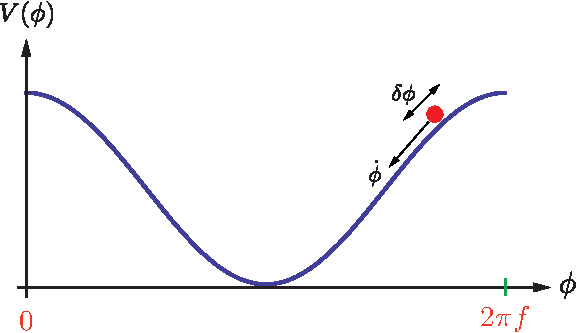
\includegraphics[width=0.5\textwidth]{NaturalInflation}
   \caption{\small ナチュラル・インフレーション．周期$2\pi f$がプランク質量を超える場合，この模型は大きな重力波振幅を自然に実現できる．}
    \label{fig:natural}
\end{figure}

\end{enumerate}
%\subsectionlink{Initial Conditions and Inflationary Attractors}

%\subsubsection{The Overshoot Problem}

%phase space

%\subsubsection{The Patch Problem}

%relation to event horizon


\subsubsection{単一場スローロールを超えて}


インフレーション膨張を得るための可能性は，（いら立たしいほどに）多様である．
インフレーションは一つのパラダイム，初期宇宙の理論の枠組みであるが，一意な理論ではない．
異なる理論的動機と観測的予言を持つ，多数の現象論的模型が提案されている．
本講義の大部分では，今述べた最も単純な単一場スローロール模型に焦点を当てる．
しかし，この短い節では，インフレーションの模型構築のより広い全体像に触れないという罪を，少しでも免れたい（文献\cite{LythRiotto}も参照）．

最も単純なインフレーションの作用(\ref{equ:simple})は，いくつかの明白な方法で拡張できる．

\begin{enumerate}
\item {\it 重力との非最小結合．}

作用(\ref{equ:simple})は，インフラトン場と計量の直接的な結合がないという意味で，最小結合と呼ばれる．原理的には，インフラトンと重力子の間の非最小結合を考えてもよい．しかし実際には，非最小結合理論は，場の再定義によって最小結合理論として書ける．

\item {\it 修正重力．}

同様に，作用のアインシュタイン・ヒルベルト部分が高エネルギーで修正される可能性も考えられる．しかし，このような重力の紫外での修正の最も単純な例である，いわゆる$f(R)$理論も，ポテンシャル$V(\phi)$を持つ最小結合スカラー場へと変換できる．

\item {\it 非正準運動項．}

作用(\ref{equ:simple})は，正準運動項を持つ．
\beq
{\cal L}_\phi = X - V(\phi)\, , \qquad X \equiv \frac{1}{2} g^{\mu \nu} \partial_\mu \phi \partial_\nu \phi\, .
\eeq
この場合，インフレーションは，ポテンシャル$V(\phi)$が非常に平坦なときにしか起こらない．
しかし，より一般には，高エネルギーの理論に，非正準運動項を持つ場が含まれることを考えられる．
\beq
\label{equ:kin}
{\cal L}_\phi = F(\phi, X) - V(\phi)\, , 
\eeq
ここで$F(\phi,X)$は，インフラトン場とその微分の何らかの関数である．
(\ref{equ:kin})のような作用では，インフレーションが運動項によって駆動され，急なポテンシャルがあっても起こりうる．

\item {\it 複数の場．}

インフレーション中に複数の場が力学的に重要であることを許すと，インフレーションの力学（および揺らぎの生成機構）の可能性は飛躍的に広がり，理論はその予言能力の多くを失う．
多場インフレーション模型の数多くの可能性の一部は，文献\cite{WandsMulti}で概説されている．
\end{enumerate}


%\subsubsection{Multi-Field Inflation} 


%hybrid inflation

%\subsubsection{Non-Trival Kinetic Terms}

%DBI inflation


\newpage
\sectionlink{{\sl まとめ}：第1講}

\vskip 10pt
通常のFRW宇宙論の初期条件は，高度に微調整されているように見える．
地平線問題も平坦性問題も，標準ビッグバンの進化の間，共動ハッブル半径$(aH)^{-1}$が時間とともに単調に増大するという事実に起因する．
一方，インフレーション中には共動ハッブル半径が一時的に減少する．
\begin{figure}[h!]
	\centering
		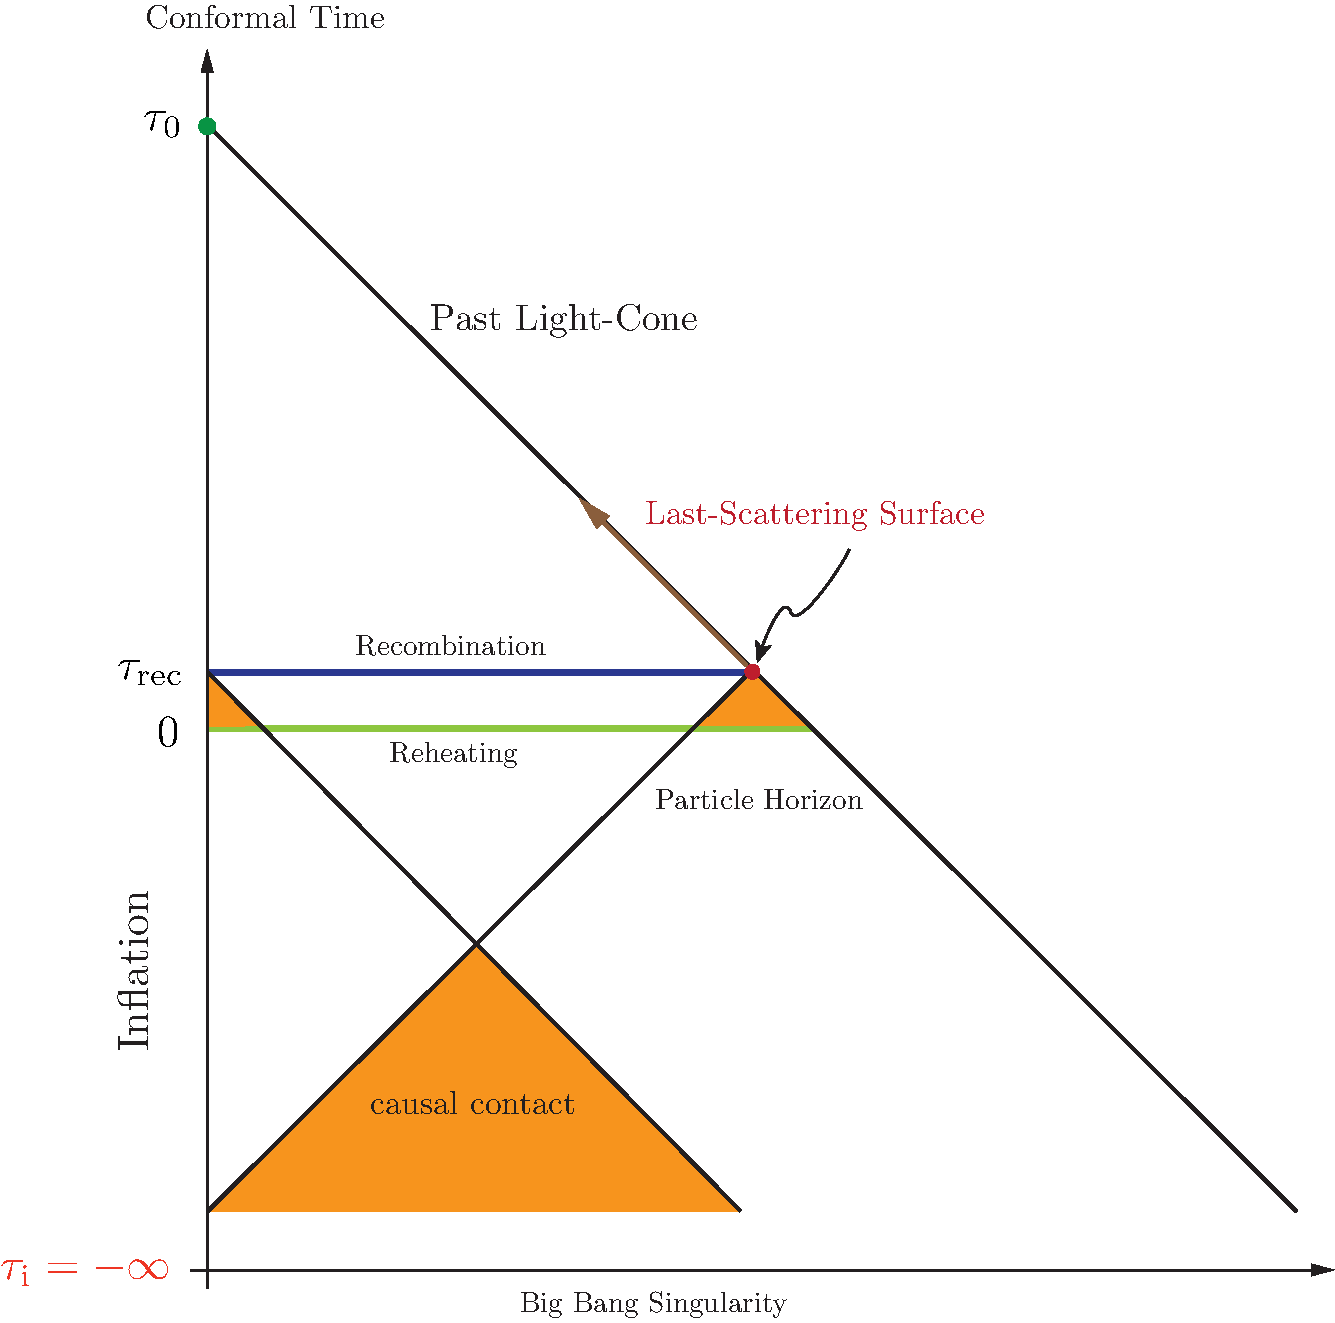
\includegraphics[width=0.55\textwidth]{InflationHorizon}
\caption{インフレーション宇宙論の共形図．インフレーションは共形時間を負の値へと拡張する！ インフレーションの終了は，$\tau = 0$に「見かけの」ビッグバンを作り出す．しかし$\tau =0$に特異点はなく，インフレーションが少なくとも60 $e$-fold続けば，光円錐はより早い時刻で交わる．}
		\label{fig:Conformal3}
\end{figure}
これによって初期宇宙の因果構造が変わり，地平線問題は，通常のFRW膨張を任意に早い時刻まで外挿することによって生じた見かけの問題となる．
アインシュタイン方程式から，ハッブル半径の縮小は加速膨張に対応し，それが負の圧力を持つ成分で宇宙が満たされている場合に生じることを示せる．
したがって，インフレーションの三つの同値な条件は，
\beq
\frac{d (aH)^{-1}}{dt}\ < \ 0 \qquad \Rightarrow \qquad \frac{d^2 a}{d t^2} \ > \ 0 \qquad \Rightarrow \qquad p\ < \ - \frac{\rho}{3} \ \ . \nonumber
\eeq
である．負の圧力を持つ流体は，次の作用を持つスカラー場$\phi$，すなわちインフラトンによって模型化できる．
\beq
S = \int \d^4 x \sqrt{-g} \left[ \frac{1}{2}R + \frac{1}{2} g^{\mu \nu} \partial_\mu \phi \partial_\nu \phi - V(\phi) \right]\, . \nonumber
\eeq
スローロール条件が満たされれば，これはインフレーションを引き起こす．
\beq
\epsilon_{\rm v} = \frac{\Mp^2}{2} \left(\frac{V_{, \phi}}{V} \right)^2\, , \qquad \eta_{\rm v} = \Mp^2 \frac{V_{, \phi \phi}}{V}\, , \qquad \quad \epsilon_{\rm v}, |\eta_{\rm v}| < 1\, . \nonumber
\eeq
このとき，インフレーションによる膨張の$e$-fold数は，
\beq
N(\phi) = \int_{\rm \phi_{\rm end}}^\phi \frac{\d \phi}{\sqrt{2 \epsilon_{\rm v}}}\, .
\eeq
である．地平線問題を解くには，総$e$-fold数が少なくとも60必要である．
CMBの揺らぎは，インフレーション終了の約60 $e$-fold前に，4 $e$-foldの間に生成される．
上記の作用で記述される単一場スローロール・インフレーションという限られた枠組みの中でも，インフレーション・ポテンシャル$V(\phi)$の異なる選び方によって特徴付けられる，多数のインフレーション模型がある．



\sectionlink{{\sl 問題集}：第1講}

\vskip 10pt
\begin{thmP}[一様かつ等方的な空間]\label{pro:FRW}
一様かつ等方的な空間は，並進不変性と回転不変性によって特徴付けられる．
3次元では，単純な位相を持つ一様かつ等方的な空間は，次の3種類しか存在しないことを確認せよ．
\begin{enumerate}
\item[i)] 平坦な空間
\item[ii)] 正の一定曲率を持つ3次元球面
\item[iii)] 負の一定曲率を持つ3次元双曲空間．
\end{enumerate}
2次元の類例の方が，視覚的に捉えやすい．
3次元ユークリッド空間への2次元球面の埋め込みを考えよう．
\beq
x^2 + y^2 + z^2 = a^2\, ,
\eeq
ここで$a$は球面の半径である．
球面上の誘導計量が，次のようになることを示せ．
\beq
\d \ell_2^2 = \frac{\d r'^2}{1-(r'^2/a^2)} + r'^2 \d \phi^2\, , 
\eeq
ここで$x=r' \cos \phi$および$y=r' \sin \phi$である．
極限$a^2 \to \infty$は，平坦な空間（平面）に対応する．
負の$a^2$は，負の一定曲率を持つ空間に対応する．
これは3次元ユークリッド空間に埋め込むことはできない．（代わりに，計量$\d \ell_2^2 = \d x^2 + \d y^2 - \d z^2$を持つ空間への，$x^2 + y^2 -z^2 =-a^2$の埋め込みを考えよ．）

動径座標を再スケールすると，計量は次の形にできる．
\beq
\d \ell_2^2 = |a^2| \left(\frac{\d r^2}{1-k r^2} + r^2 \d \phi^2 \right)\, ,
\eeq
ここで，球面（$a^2 > 0$）では$k=+1$，双曲空間（$a^2 < 0$）では$k=-1$，平面（$a^2 =0$）では$k=0$である．

上の議論を，一様かつ等方的な3次元空間の4次元ユークリッド空間への埋め込みに一般化せよ．その計量が次のようになることを示せ．
\beq
\d \ell_3^2 = a^2 \left(\frac{\d r^2}{1-k r^2} + r^2 \d \Omega^2 \right)\, , \qquad \d \Omega^2 \equiv \d \theta^2 + \sin^2 \theta \d \phi^2\, ,
\eeq
あるいは，
\beq
\d \ell_3^2 = a^2 \left[\d \chi^2 +\left( 
\begin{array}{c} \sinh^2 \chi \\ \chi^2 \\ \sin^2 \chi \\
\end{array} \right) \d \Omega^2\right] \quad \begin{array}{l} k=-1 \\ k=0 \\ k=+1 \end{array} \, .
\eeq
空間の一様性と等方性を保つ，時間依存する唯一の4次元時空が，FRW計量であることを確認せよ．
\beq
\d s^2 = \d t^2 - a^2(t)  \left(\frac{\d r^2}{1-k r^2} + r^2 \d \Omega^2 \right)\, .
\eeq
\end{thmP}

\begin{thmP}[共形時間]
共形時間$\tau$を$a$の関数として表す，いくつかの簡単な式を導け．

\begin{enumerate}
\item 物質優勢宇宙では$\tau \propto a^{1/2}$，放射優勢宇宙では$\tau \propto a$となることを示せ．
\item 物質と放射のみを含み，$a_{\rm eq}$で両者が等しくなる宇宙を考えよ．次を示せ．
\beq
\label{equ:taueq}
\tau = \frac{2}{\sqrt{\Omega_m H_0^2}} \left[ \sqrt{a+a_{\rm eq}} - \sqrt{a_{\rm eq}}\right]\, .
\eeq
現在の共形時間はいくらか．脱結合時にはいくらか．
\item 好みのソフトウェア（例えばMathematicaやMaple）を使って，私たちの宇宙（ダークエネルギー，物質，放射で満たされている）の共形時間を数値的に計算せよ．現在と脱結合時の共形時間を求めよ．この結果と，物質・放射のみの宇宙に対する解析的結果である式~(\ref{equ:taueq})の誤差は，何パーセントか．
\end{enumerate}
\end{thmP}

\begin{thmP}[フリードマン方程式]\label{pro:Friedmann}
FRW時空(\ref{equ:FRW})のリッチ・テンソルとリッチ・スカラーを導け．
\beq
R_{00} = -3 \frac{\ddot a}{a}\, , \qquad R_{ij} = \delta_{ij} \left[2 \dot a^2 + a \ddot a + 2\frac{k}{a^2} \right]\, , \qquad R= g^{\mu \nu} R_{\mu \nu} = 6 \left[\frac{\ddot a}{a} + \left(\frac{\dot a}{a}\right)^2 + \frac{k}{a^2}\right]\, .
\eeq
アインシュタイン方程式(\ref{equ:Einstein})の00成分が，フリードマン方程式を与えることを確かめよ．
\beq
\left(\frac{\dot a}{a}\right)^2 =  \frac{8\pi G}{3} \rho - \frac{k}{a^2} \, .
\eeq
アインシュタイン方程式(\ref{equ:Einstein})のトレースが，加速度方程式を与えることを確かめよ．
\beq
\frac{\ddot a}{a} = - \frac{4\pi G}{3} (\rho + 3 p) \, .
\eeq
2本のフリードマン方程式から，連続の式が従うことを示せ．
\beq
\dot \rho = - 3H (\rho + p)\, .
\eeq
次の式から連続の式を導け．
\beq
\label{equ:conservation}
\nabla_\mu T^\mu_{\ \nu} = 0\, .
\eeq
（ヒント：式~(\ref{equ:conservation})を$U^\mu$と縮約し，完全流体のエネルギー運動量テンソルと4元速度の性質を使え．クリストッフェル記号は不要である！）
\end{thmP}

%\begin{thm}[Scalar Fluid]
%From the scalar field action derive the energy-momentum tensor
%\beq
%T_{\mu \nu} =
%\eeq
%Show that in the homogeneous limit, $\phi(t, {\bf x}) \to \phi(t)$ this takes the form of a perfect fluid (x.x) with
%\beq
%\rho = \frac{1}{2}\dot \phi^2 + V(\phi)\, , \qquad p=\frac{1}{2}\dot \phi^2 - V(\phi)\, .
%\eeq
%\end{thm}

%\begin{thm}[Preheating]
%\end{thm}

\begin{thmP}[$\lambda \phi^4$インフレーション]\label{pro:case}
$\lambda \phi^4$インフレーションのスローロール力学を導け．
\end{thmP}


\begin{thmP}[$m \phi^2$インフレーションの位相空間]\label{pro:case2}
Mukhanovの教科書\cite{Mukhanov}で，$m^2 \phi^2$インフレーションのアトラクターとしての振る舞いについて読め．
\end{thmP}


\newpage



\part{第2講：インフレーション中の{\sl 量子}揺らぎ}


\vspace{0.5cm}
 \hrule \vspace{0.3cm}
\begin{quote}
{\bf 要旨}

\noindent
本講では，インフレーション中の量子揺らぎが生成する原始揺らぎのスペクトルについて，よく知られた計算を示す．
計算の細部をすべて示し，「ごまかし」や近似をできるだけ避ける．
宇宙論的摂動論の基礎を簡単に復習した後，まず，インフレーションが微視的な量子揺らぎを宇宙の構造形成の巨視的な種へ変換する基本機構を定性的にまとめる．
次に，曲がった時空における場の量子論への教育的な導入として，単純調和振動子の量子化を復習する．真空が最低エネルギー状態であることを要求すると，真空状態が一意に選ばれる点を強調する．
続いて，インフレーションについて対応する計算を行う．
スカラー揺らぎとテンソル揺らぎの両方のパワースペクトルを計算し，そのスケール依存性を論じる．

\end{quote}
\vspace{0.1cm}  \hrule
 \vspace{1.5cm}



前講では，ポテンシャルを速度$\dot \phi$で転がり落ちるスカラー場の古典的（$\hbar =0$）な力学を調べた（図\ref{fig:small2}参照）．本講では，古典的な背景の時間発展$\bar \phi(t)$の周りの量子（$\hbar \ne 0$）揺らぎの効果を調べる．この揺らぎは，インフレーションの終了時刻に局所的な遅延を生む．すなわち，宇宙の異なる領域では，インフレーションがわずかに異なる時刻に終わる．例えば，図\ref{fig:small2}のポテンシャルでは，凍結した負の揺らぎ$\delta \phi$を獲得した領域は，正の$\delta \phi$をもつ領域より長くポテンシャルが支配的な状態にとどまる．
したがって，宇宙の異なる領域はわずかに異なる時間発展をたどる．これが相対的な密度揺らぎ$\delta \rho(t, {\bf x})$を生む．
%These fluctuations persist after inflation and provide the initial conditions for the formation of large-scale structures.

\begin{figure}[htbp]
    \centering
        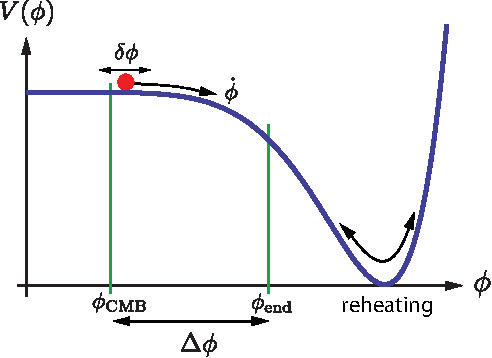
\includegraphics[width=0.4\textwidth]{SmallField}
   \caption{\small 古典的な背景の時間発展$\bar \phi(t)$の周りの量子揺らぎ$\delta \phi(t, {\bf x})$．}
    \label{fig:small2}
\end{figure}

本講では，大規模構造の量子的起源についてのこの基本描像を支える技術的な詳細を論じる．


\begin{figure}[h!]
    \centering
        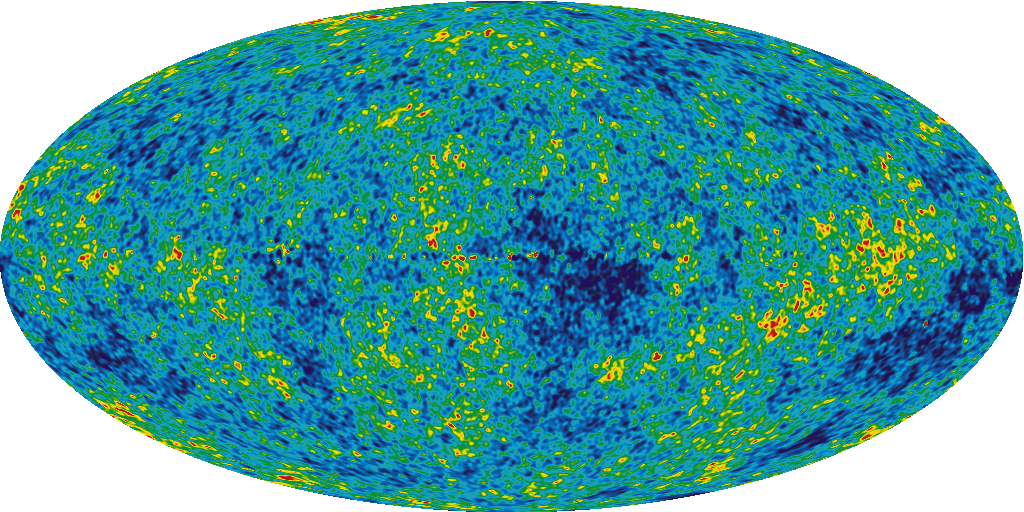
\includegraphics[width=0.7\textwidth]{cmb.png}
    \caption{\small CMBの異方性の観測は，初期宇宙が完全には一様でなかったことを示している．
    一方，その非一様性が小さく，一様な背景の周りの線形摂動として解析できることも観測からわかる．} % (see Figures \ref{fig:WMAP2} and \ref{fig:CMBparam}).}
    \label{fig:cmb}
\end{figure} 



\sectionlink{{\sl 復習}：宇宙論的摂動}

本講では，インフレーション中の量子揺らぎから宇宙論的摂動が生成される過程を詳しく示す．
この議論には宇宙論的摂動論の予備知識が必要なので，ここで簡単に復習する．
さらに詳しい説明は付録Aにある．
%In this section we give a general summary of cosmological perturbation theory. % \cite{Brandenberger:1993zc, Kodama:1985bj, Malik:2008im}. 
%In Section \ref{sec:qf} we then describe how these fluctuations arise as quantum fluctuations during the inflationary epoch.


%\subsectionlink{Linear Theory}





\subsectionlink{一般的事項}

\subsubsection{線形摂動}
CMBの観測（図\ref{fig:cmb}）は，宇宙論的摂動論が成功する理由を教えてくれる．
脱結合の時代の宇宙はほぼ一様で，非一様性は$10^{-5}$程度と小さかった．
したがって自然な方針は，すべての量$X(t, {\bf x})$（計量$g_{\mu \nu}$および物質場$T_{\mu \nu}$ $\to$ $\phi$ $\rho$, $p$など）を，宇宙時刻だけに依存する一様な背景$\bar X(t)$と，空間に依存する摂動とに分けることである．
\beq
\label{equ:pert}
\delta X(t, {\bf x}) \equiv X(t, {\bf x}) - \bar X(t)\, .
\eeq
摂動は小さいので，$\delta X \ll \bar X$，アインシュタイン方程式を摂動の線形次数まで展開すると，完全な非線形解を非常によい精度で近似できる．
\beq
\delta G_{\mu \nu} = 8\pi G\, \delta T_{\mu \nu}\, .
\eeq



\subsubsection{ゲージの選択}
宇宙論的摂動を調べる際の重要で微妙な点は，式(\ref{equ:pert})の背景と摂動への分割が一意ではなく，座標の選択，すなわち{\it ゲージの選択}に依存することである．\footnote{テンソル場$X$で表される任意の量の摂動$\delta X$は，物理的時空（摂動を受けた時空）での$X$の値と，与えられた（摂動のない）背景時空での同じ量の値$X_0$との差として定義される．しかし，テンソルの比較を意味のあるものとするには，この二つの異なる時空の点を同一視する処方が与えられてからでなければ比較できない，というのが微分幾何学の基本的な事実である．{\it ゲージの選択}とはまさにこのこと，すなわち背景時空と物理的時空の間の一対一の対応（写像）を与えることである．この写像の変更がゲージ変換であり，その選択の自由度によって，$X$がゲージ不変でない限り，任意の時空点における$X$の摂動の値には任意性が生じる．}
{\bf 第1講}で一様な宇宙を記述した際には，座標$t$と${\bf x}$を導入してFRW計量を定義した．
時刻$t$が一定の空間的超曲面が4次元時空の{\it スライシング}を定め，一方，${\bf x}$が一定の時間的世界線が{\it スレッディング}を定めた．
FRWのスレッディングは，自分の位置で運動量密度がゼロとなる共動観測者の運動に対応する．この観測者は自由落下し，彼らが定義する膨張は等方的である．スライシングはスレッディングに直交し，それぞれの空間的切片が一様な宇宙に対応する．
これらの特徴により，この座標の選択は際立って特別なものとなり，他の座標（そこでは宇宙が一様・等方には見えない）を気にする必要はなかった．
しかし，摂動を考える今は，摂動を受けた時空のスライシングとスレッディングが一意ではないことを認識するのが重要である．さらに，非一様な時空を記述する際には，特に好ましい座標の選び方が存在しないことも多い．
時空のスライシングとスレッディングを定めるためにゲージを選ぶと，暗黙のうちに摂動も定義している．
注意しないと，この摂動のゲージ依存性は混乱を招きうる．
このことを最も鮮明に示すため，エネルギー密度が時刻だけの関数$\rho(t, {\bf x})= \rho(t)$である，{\it 摂動のない}一様・等方な宇宙を考えよう．
ここで，時間座標の変更が{\it 見かけの}摂動$\delta \rho$を導入しうることを示す．新しい時間座標$\tilde t = t + \delta t(t, {\bf x})$を考える．一般に，新しい時間切片上ではエネルギー密度は一様ではなく，$\tilde \rho(\tilde t, {\bf x})= \rho(t(\tilde t, {\bf x}))$となる．このエネルギー密度の摂動は物理的なものではなく，すべて新しい時間スライシングの選択による．
同様に，時刻一定の超曲面をエネルギー密度一定の超曲面に一致させて選ぶと，エネルギー密度の{\it 実際の}摂動を取り除ける．このとき，実際に非一様性が存在していても$\delta \tilde \rho=0$となる．
一般相対論における実際の摂動と見かけの摂動の曖昧さを解消するには，摂動の完全な組を考える必要がある．すなわち，物質場の摂動と計量の摂動を両方考える必要があり，ゲージ変換によって一方を他方へ移し替えられる．
見かけのゲージモードの誤解を避けるには，摂動のゲージ不変な組合せを調べることも有用である．定義から，ゲージ不変量の揺らぎは座標変換で取り除けない．


\subsubsection{スカラー，ベクトル，テンソル}
空間的に平坦で一様・等方な背景時空は，多くの対称性をもつ．この対称性によって，計量とエネルギー運動量の摂動を
%associated with $\phi$ 
独立なスカラー（S），ベクトル（V），テンソル（T）成分に分解できる．この{\it SVT分解}はフーリエ空間で最も簡単に記述できる．
\beq
 X_{\bf k}(t) = \int \d^3 {\bf x} \  X(t, {\bf x}) \, e^{i {\bf k} \cdot {\bf x}}\, , \qquad X \equiv \delta \phi,\, \delta g_{\mu \nu}, \text{など}\, .
\eeq 摂動に対する線形運動方程式の{\it 並進不変性}は，異なるフーリエモードが相互作用しないことを意味する点に注意しよう（証明は付録\ref{sec:CPT}参照）．
したがって，異なるフーリエモードは独立に調べられる．これにより，摂動の微分方程式が簡単になることが多い．
次に，一つのフーリエ波数ベクトル${\bf k}$の周りの回転を考える．座標系を波数ベクトルの周りに角度$\psi$だけ回転したとき，その振幅に$e^{i m \psi}$が掛かる摂動は，ヘリシティ$m$をもつという．
\beq X_{\bf k} \to e^{im \psi} X_{\bf k}\, .
\eeq スカラー，ベクトル，テンソル摂動のヘリシティは，それぞれ$0$，$\pm 1$，$\pm 2$である．\footnote{ヘリシティによるこの抽象的なスカラー，ベクトル，テンソル摂動の定義がわかりにくければ，次節で導入する具体的な計量およびエネルギー運動量の摂動について，これらの規則を確かめてみるとよい．}SVT分解の重要な点は，それぞれの種類の摂動が（線形の範囲では）独立に時間発展し，したがって別々に扱えることである（証明は付録\ref{sec:CPT}参照）．
これにより，宇宙論的摂動の解析は大幅に簡単になる．

\vskip 8pt
以上の一般的な説明を踏まえ，さらに具体的に，一様・等方なFRW宇宙の周りの摂動を明示的に定義しよう．

%\subsectionlink{Metric and Stress-Energy Perturbations}

\subsectionlink{非一様な宇宙}

\subsubsection{計量摂動}
インフレーション中には，インフラトン$\bar \phi(t)$と計量$\bar g_{\mu \nu}(t)$の一様な背景解の周りで摂動を定義する．
\beq \phi(t, {\bf x}) = \bar \phi(t)
+ \delta \phi(t, {\bf x})\, , \qquad g_{\mu \nu}(t, {\bf x}) = \bar g_{\mu \nu}(t) + \delta g_{\mu \nu}(t, {\bf
x})\, , \eeq 
ここで，
\bea
\d s^2 &=& g_{\mu \nu}\, \d x^\mu \d x^\nu \nonumber \\
&=& -(1+2 \Phi) \d t^2 + 2 a B_i \d x^i \d t + a^2 [(1-2 \Psi) \delta_{ij} + E_{ij}] \d x^i \d x^j\, .
\label{equ:perturbed} 
\eea
実空間での計量摂動(\ref{equ:perturbed})のSVT分解は次のようになる．\footnote{実空間でのSVT分解は，空間的超曲面上でのスカラー，ベクトル，テンソルの異なる変換性に対応する．}
\beq \label{equ:SVT1} B_i \equiv
\partial_i B- S_i\, , \qquad \text{ただし} \quad  \partial^i S_i = 0\, , \eeq また，\beq \label{equ:SVT2}
 E_{ij} \equiv 2 \partial_{ij} E + 2 \partial_{(i} F_{j)} + h_{ij}\, ,  \qquad \text{ただし} \quad \partial^i F_i =0\, , \quad h^i_{i} = \partial^i h_{ij} = 0\, .
\eeq
ベクトル摂動$S_i$と$F_i$はインフレーションでは生成されない（いずれにせよ宇宙の膨張とともに減衰する）．この理由から，本講義ではベクトル摂動を無視する．
以下では，後期宇宙で密度揺らぎと重力波として観測されるスカラー揺らぎとテンソル揺らぎに注目する．

テンソル揺らぎはゲージ不変だが，スカラー揺らぎは座標の変更に伴って変化する．
次のゲージ変換を考える．
\bea
t &\to& t + \alpha \\
x^i &\to& x^i + \delta^{ij} \beta_{,j}\, .
\eea
この座標変換の下で，スカラー計量摂動は次のように変換される．
\bea
\Phi &\to& \Phi - \dot \alpha\label{equ:d1} \\
B &\to& B + a^{-1} \alpha - a \dot \beta \\
E &\to& E - \beta \\
\Psi &\to& \Psi + H \alpha\, . \label{equ:d2}
\eea

\begin{thm}[線形ゲージ変換]
スカラー計量摂動のゲージ変換(\ref{equ:d1})--(\ref{equ:d2})を導け．ヒント：時空間隔の不変性を用いよ．
\beq
\d s^2 = g_{\mu \nu} \d x^\mu \d x^\nu = \tilde g_{\mu \nu} \d \tilde x^\mu \d \tilde x^\nu\, .
\eeq
\label{ex:gauge}
\end{thm}

\subsubsection{物質摂動}
インフレーション中には，インフレーションのエネルギーが宇宙のエネルギー運動量への支配的な寄与を与えるため，インフラトンの摂動$\delta \phi$は時空幾何に逆反応する．
この物質摂動と計量摂動の結合は，アインシュタイン方程式によって記述される（付録\ref{sec:CPT}参照）．

インフレーション後，宇宙の全エネルギー運動量テンソルの摂動は次のようになる．
\bea
T^0_0 &=& - (\bar \rho + \delta \rho) \\
T^0_i &=& (\bar \rho +\bar p)\, av_i \\
T^i_0 &=& -(\bar \rho + \bar p) (v^i - B^i)/a \\
T^i_j &=& \delta^i_j (\bar p + \delta p) + \Sigma^i_j\, .
\eea
異方性応力$\Sigma^i_j$はゲージ不変である一方，密度，圧力，運動量密度（$(\delta q)_{,i} \equiv (\bar \rho + \bar p) v_i$）は次のように変換される．
\bea
\delta \rho &\to& \delta \rho - \dot {\bar \rho} \,\alpha \\
\delta p &\to& \delta p - \dot {\bar p}\, \alpha \\
\delta q &\to& \delta q + (\bar \rho + \bar p)\, \alpha\, .
\eea



\subsubsection{ゲージ不変変数}

上で説明したように，見かけのゲージモードという落とし穴を避けるには，計量摂動と物質摂動のゲージ不変な組合せを導入すると便利である\cite{Bardeen:1980kt}．
重要なゲージ不変スカラー量の一つは，{\it 一様密度超曲面上の曲率摂動}である\cite{BST}．
\beq
\fbox{$\displaystyle
\label{equ:zeta} - \zeta \equiv  \Psi +  \frac{H}{\dot{\bar \rho}}
\delta \rho $} \, .
\eeq
%where $\rho$ is the total energy density of the universe.
幾何学的には，$\zeta$は密度一定の超曲面の空間曲率$R^{(3)} = 4 \nabla^2 \Psi/a^2$を測る．$\zeta$の重要な性質は，断熱的な物質摂動，すなわち次式を満たす摂動に対して，地平線の外側で一定にとどまることである．
\beq
\label{equ:ad:source-duplicate-1}
\fbox{$\displaystyle
\delta p_{en} \equiv \delta p - \frac{\dot {\bar p}}{\dot {\bar \rho}} \delta \rho $} = 0\, .
\eeq
$\delta p_{en}$の定義がゲージ不変であることに注意しよう．
本講で扱う単一場インフレーション模型では条件(\ref{equ:ad})が常に満たされるので，摂動$\zeta_{\bf k}$は地平線の外側$k \ll aH$では時間発展しない．


空間的に平坦な超曲面$\Psi$で定義されるゲージでは，摂動$\zeta$は無次元の密度摂動$\frac{1}{3} \delta \rho/(\bar \rho+ \bar p )$である．
%On sub-horizon scales $\zeta$ is related to density perturbations $\delta \rho$.
したがって，地平線内での揺らぎの時間発展を記述する適切な伝達関数を考慮すると，CMBおよび大規模構造（LSS）の観測を$\zeta$の原始的な値に結び付けられる（{\bf 第3講}参照）．
スローロール・インフレーション中には，
\beq
\label{equ:zetaSR}
- \zeta \approx \Psi + \frac{H}{\dot{\bar \phi}} \delta \phi\, .
\eeq

もう一つのゲージ不変スカラーは{\it 共動曲率摂動}である．
\beq
\fbox{$\displaystyle
{\cal R} \equiv \Psi - \frac{H}{\bar \rho + \bar p} \delta q $}\, ,
\eeq
ここで，$\delta q$は3次元運動量密度$T^0_i = \partial_i \delta q$のスカラー部分である．
インフレーション中には$T^0_i = - \dot{\bar \phi}\, \partial_i \delta \phi$なので，
\beq
\label{equ:RSR}
\R = \Psi + \frac{H}{\dot{\bar \phi}} \delta \phi\, .
\eeq
幾何学的には，${\cal R}$は共動超曲面（または$\phi$一定の超曲面）の空間曲率を測る．%, $R^{(3)} = -4 \nabla^2 {\cal R}/a^2$.

線形化したアインシュタイン方程式は，$\zeta$と${\cal R}$を次のように関係付ける（付録\ref{sec:CPT}参照）．
\beq
-\zeta = {\cal R} + \frac{k^2}{(aH)^2} \frac{2 \bar \rho}{3(\bar \rho + \bar p)} \Psi_{\rm B}\, ,
\eeq
ここで，
\beq
\Psi_{\rm B} \equiv \psi + a^2 H (\dot E - B/a)\, ,
\eeq
はバーディーン・ポテンシャルの一つである\cite{Bardeen:1980kt}．
したがって，$\zeta$と${\cal R}$は地平線より大きなスケール$k \ll aH$で等しい．
また，$\zeta$と${\cal R}$はスローロール・インフレーション中にも等しい．式(\ref{equ:zetaSR})と(\ref{equ:RSR})を参照．
したがって，$\zeta$と$\R$の相関関数は地平線通過時に等しく，$\zeta$と$\R$はいずれも地平線より大きなスケールで保存される．
本講では，地平線通過時の$\R$の原始スペクトルを計算する．

最後に，インフラトン摂動のゲージ不変な尺度は，{\it 空間的に平坦な切片上のインフラトン摂動}である．
\beq
\fbox{$\displaystyle
Q \equiv \delta \phi + \frac{\dot {\bar \phi}}{H}\Psi $}\, .
\eeq

\begin{thm}[ゲージ不変な摂動]
計量摂動と物質摂動の線形ゲージ変換を用い，$\zeta$，$\R$，$Q$がゲージ不変であることを確かめよ．
\label{ex:gauge2}
\end{thm}


\subsubsection{地平線より大きなスケールでの時間発展（とその不在）}


アインシュタイン方程式（付録\ref{sec:CPT}参照）は，ゲージ不変な曲率摂動に対して次の時間発展方程式を与える．
\beq
\dot \R = -  \frac{H}{\bar \rho + \bar p}\, \delta p_{en} + \frac{k^2}{(aH)^2} \Bigl(\dots \Bigr)\, .
\eeq
断熱的な物質摂動は$\delta p_{en} =0$を満たし，$\R$は地平線より大きなスケール$k < aH$で保存される．

\begin{thm}[別個の宇宙のアプローチ]
地平線より大きなスケールにおける曲率摂動$\R$の保存を証明する，別個の宇宙のアプローチ\cite{Wands:2000dp}について読め．
\label{ex:separate:source-duplicate-1}
\end{thm}


\subsectionlink{宇宙論的摂動の統計}


原始スカラー揺らぎの重要な統計的尺度は，$\R$（または$\zeta$）のパワースペクトルである．\footnote{無次元パワースペクトル$\Delta_\R^2(k)$の規格化は，$\R$の分散が$\langle \R \R \rangle = \int_0^\infty \Delta_\R^2(k) \, \d \ln k$となるように選んでいる．}
\beq \langle \R_{\bf k} \R_{{\bf k}'}
\rangle = (2\pi)^3 \, \delta({\bf k} + {\bf k}') \, P_\R(k)\, , \qquad \Delta_{\rm s}^2 \equiv \Delta_\R^2 = \frac{k^3}{2\pi^2} P_\R(k)\, .  \eeq
%\beq \langle \zeta_{\bf k} \zeta_{{\bf
%k}'} \rangle = (2\pi)^3 \delta({\bf k} + {\bf k}') {\cal P}_s(k)\, , \qquad P_s(k) \equiv \frac{k^3}{2 \pi^2}
%{\cal P}_s(k) \eeq
ここで，$\langle \, ...\, \rangle$は揺らぎのアンサンブル平均を表す．
パワースペクトルのスケール依存性は，スカラー・スペクトル指数（または傾き）によって定義される．\beq
\label{equ:ns}
n_{\rm s} - 1 \equiv \frac{d
\ln \Delta^2_{\rm s}}{d \ln k}\, ,\eeq
ここで，スケール不変性は$n_{\rm s} = 1$に対応する．スペクトル指数のランニングも次のように定義できる．\beq \label{equ:as}
 \alpha_{\rm s}
\equiv \frac{d n_{\rm s}}{d \ln k}\, . \eeq
パワースペクトルは，しばしば次のべき乗則の形で近似される．
\beq
\Delta_{\rm s}^2(k) = A_{\rm s}(k_\star) \left(\frac{k}{k_\star}\right)^{n_{\rm s}(k_\star)-1+ \frac{1}{2} \alpha_{\rm s}(k_\star) \ln (k/k_\star)}\, ,
\eeq
ここで，$k_\star$は任意の基準スケール，またはピボットスケールである．

$\R$がガウス的なら，パワースペクトルはすべての統計的情報を含む．原始非ガウス性は，$\R$の高次相関関数に符号化されている．
%(see \S\ref{sec:NG}).
単一場スローロール・インフレーションでは，非ガウス性は小さいと予言される\cite{Acquaviva02,malda}．
しかし，多場模型や，非自明な運動項をもつ，あるいはスローロール条件を破る単一場模型では，非ガウス性が大きくなることがある．
原始非ガウス性には{\bf 第4講}で戻る．本講では，計算をガウス揺らぎとそれに伴うパワースペクトルに限る．


$h_{ij}$の二つの偏極モード，すなわち$h \equiv h^+, h^\times$のパワースペクトルは次のように定義される．\beq \langle h_{\bf k} h_{{\bf k}'} \rangle = (2\pi)^3\, \delta({\bf
k} + {\bf k}')\, P_h(k)\, , \qquad \Delta_h^2 = \frac{k^3}{2\pi^2} P_h(k)\, .  %\qquad P_t(k) \equiv \frac{k^3}{2 \pi^2} {\cal P}_t(k)
\eeq
テンソル摂動のパワースペクトルを，二つの偏極のパワースペクトルの和として定義する．
\beq
\Delta_{\rm t}^2 \equiv 2 \Delta_h^2\, .
\eeq
そのスケール依存性は式(\ref{equ:ns})と同様に定義されるが，歴史的理由から$-1$を付けない．
\beq n_{\rm t} \equiv \frac{d \ln \Delta^2_{\rm t}}{d \ln k}\, , \eeq
すなわち，
\beq
\Delta^2_{\rm t}(k) = A_{\rm t}(k_\star) \left(\frac{k}{k_\star}\right)^{n_{\rm t}(k_\star)}\, .
\eeq

%CMB polarization measurements are sensitive to the ratio of tensor  power to scalar power \beq r \equiv \frac{P_t}{P_s}  \, . \eeq The parameter $r$ will be of fundamental
%importance for the discussion presented in this paper.
%As we argue in Section \ref{sec:Bmodes}, its value encodes crucial information about the physics
%of the inflationary era.

\vspace{0.5cm}
%\underline{\bf Aim of this lecture:} 
\subsubsection*{本講の目的}
本講の目的は，スカラー揺らぎとテンソル揺らぎのパワースペクトル$P_\R(k)$と$P_h(k)$を第一原理から計算することである．
これは現代の理論宇宙論において最も重要な計算の一つであり，理解するために努力する価値は十分にある．

%\subsectionlink{Three Gauges and $\zeta$, ${\cal R}$ and $Q$}

%\subsubsection{Uniform Density Gauge}

%define $\zeta$

%\subsubsection{Comoving Gauge}

%define ${\cal R}$

%\subsubsection{Spatially-Flat Gauge}

%define $Q$

 
%\newpage
%%%%%%%%%%%%%%%%%%%%%%%%%%%%%%%%%%
\sectionlink{{\sl 概観}：構造の量子的起源} %: A Qualitative (Pre)View}
%\sectionlink{Quantum Fluctuations as the Origin of Structure}
\label{sec:qf}
%%%%%%%%%%%%%%%%%%%%%%%%%%%%%%%%%%

%{\tt more. add some things fro Will's intro}\\


前講では，インフラトン場の古典的な時間発展を論じた．インフラトンの量子揺らぎを考えると，驚くべきことが起こる．インフレーションと量子力学を組み合わせると，宇宙のあらゆる構造の初期の種を生成する美しい機構が得られるのである．言い換えると，インフレーション中の量子揺らぎが，スカラー揺らぎとテンソル揺らぎの原始パワースペクトル$P_{\rm s}(k)$と$P_{\rm t}(k)$の源となる．
本節では，インフレーションが微視的な物理を巨視的な観測量に結び付ける機構を概説する．
\S\ref{sec:full}では完全な計算を示す．


\begin{figure}[htbp]
    \centering
        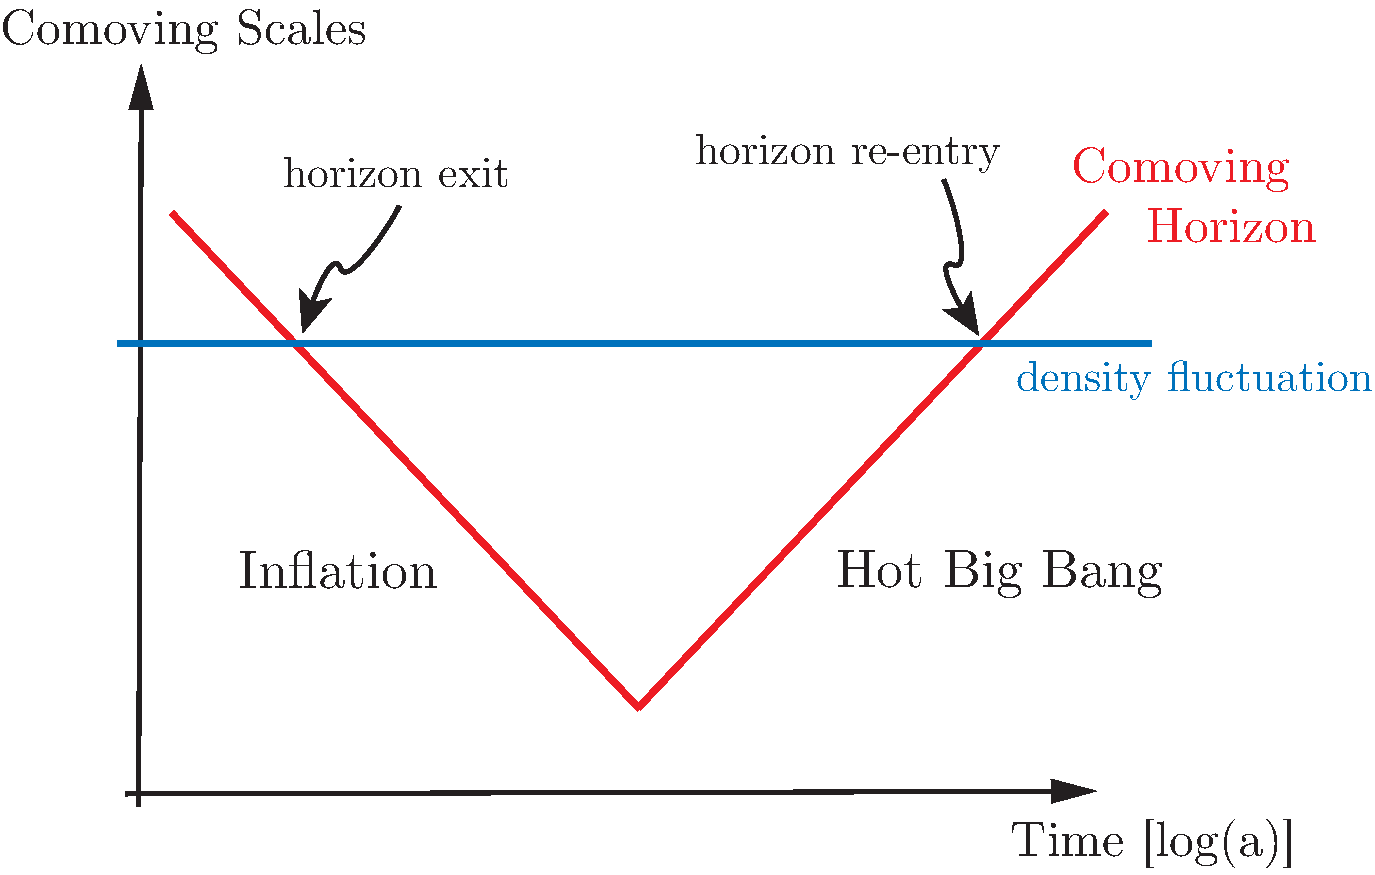
\includegraphics[width=0.65\textwidth]{./Scales}
   \caption{\small インフレーション宇宙における摂動の生成と時間発展．揺らぎは地平線内のスケールで量子力学的に生成される．共動スケール$k^{-1}$が一定に保たれる一方，インフレーション中の共動ハッブル半径$(aH)^{-1}$は縮小し，摂動は地平線の外へ出る．因果的な物理過程は地平線より大きな摂動に作用できず，摂動は後の時代に地平線へ再突入するまで凍結する．}
    \label{fig:scales}
\end{figure}

\subsectionlink{量子的な零点揺らぎ}

\S\ref{sec:full}で定量的に説明するように，インフレーション中の量子揺らぎは，すべての軽い場（インフラトンや計量摂動など）の揺らぎにゼロでない分散を生じさせる．
これは，基底状態での零点揺らぎが調和振動子の振幅に生む分散と非常によく似ている．\S\ref{sec:SHO}参照．
揺らぎの振幅は，インフレーション中の膨張パラメータ$H$に比例する．
これはド・ジッター地平線$H^{-1}$に関係しており，インフレーション中の量子揺らぎは，ブラックホールのホーキング放射との密接な類似の下で，ド・ジッター空間の熱揺らぎとして解釈することもできる．

揺らぎはすべての長さスケールで，すなわち波数$k$のスペクトルをもって生成される．
宇宙論的に重要な揺らぎは，地平線（ハッブル半径）の内側で生まれる．
\beq \text{地平線内：} \quad
k \gg aH\, .
\eeq
しかし，共動波数が一定である一方，共動ハッブル半径はインフレーション中に縮小する（これがインフレーションの「定義」であったことを思い出そう）．したがって，やがてすべての揺らぎは{\it 地平線の外へ出る}．
\beq \text{地平線外：} \quad
k < aH\, .
\eeq

\subsectionlink{地平線からの退出と再突入}

宇宙論的な非一様性は，物質に関して定義した空間的超曲面の内在的曲率$\R$または$\zeta$によって特徴付けられる．
${\cal R}$と$\zeta$はどちらも，地平線の外側，すなわち$k < aH$で一定にとどまるという便利な性質をもつ．
特に，その振幅はインフレーション直後の宇宙の未知の物理的性質の影響を{\it 受けない}（再加熱の詳細についてはほとんど何もわかっていないことを思い出そう．それでも宇宙論的観測量を予言できるのは，地平線の外側で$\R$と$\zeta$が一定であるためである）．
インフレーション後には共動地平線が成長するので，やがてすべての揺らぎは地平線へ再突入する．
地平線再突入後，$\R$または$\zeta$は宇宙流体の摂動を定め，観測されるCMB異方性とLSSをもたらす．\\ % (see Lecture 3).\\


%\subsectionlink{The Physical Importance of ${\cal R}$ and $\zeta$}


{\bf 第1講}では，インフレーション中と，その後の標準的なFRW膨張中における共動地平線の時間発展を説明した．
本講（{\bf 第2講}）では，地平線退出時の共動曲率揺らぎ$\R$の原始パワースペクトルを計算する．
次講（{\bf 第3講}）では，曲率揺らぎ$\R$と，地平線再突入後の宇宙論的観測量の揺らぎとの関係を計算する．
したがって，この三つの講義を合わせると，インフレーションが生成する量子揺らぎの生成過程と観測への帰結の両方について，完全な説明が得られる．
これは美しい物語である．その展開を始めよう．

\sectionlink{調和振動子の量子力学} %Simple
\label{sec:SHO}

\begin{quote}
「若い理論物理学者の歩みは，抽象度をますます高めながら調和振動子を扱うことからなる．」

{\it Sidney Coleman}
\end{quote}

%Since inflation stretches microscopic scales into astronomical ones, it suggests the possibility that the density perturbations which provide the seeds for galaxy formation might have originated as microscopic quantum fluctuations.
インフレーション中に生成される量子揺らぎの計算は，代数計算がかなり多い．そこで，関係する物理の大部分を含みつつ，より簡単な例から始めるのが有益である．準備として，1次元の単純調和振動子の量子化を考えよう．
調和振動子は，物理学者が厳密に解ける数少ない物理系の一つである．幸い，もっと複雑な物理系もほぼすべて，振幅と振動数の異なる単純調和振動子の集まりとして表現できる．
% (remember normal modes in classical dynamics?). 
これはもちろん，フーリエ解析そのものである．
以下では，曲がった時空（特にド・ジッター空間）における自由場が，時間に依存する振動数をもつ調和振動子の集まりに似ていることを示す．したがって，本節で量子調和振動子を詳しく扱うことは無駄ではなく，インフレーションの計算に重要な直観を与える．本節は文献\cite{Jacobson:2003vx}の優れた解説に基づく．

\subsectionlink{作用}

時間に依存する振動数をもつ調和振動子の古典作用は，
\begin{equation}
S = \int \d t \, \left(\frac{1}{2} \dot{x}^2 -\frac{1}{2} \omega^2(t) x^2 \right) \equiv \int \d t \, L\, ,
\end{equation}
ここで，$x$は平衡状態$x \equiv 0$からの粒子のずれであり，便宜上，粒子の質量を1，$m \equiv 1$とした．具体的には，外部の熱源によって加熱され，ばね定数$k(t)$が時間に依存するばねにつながれた質量$m$の粒子を考えるとよい．ただし$\omega^2 =k/m$である．古典的な運動方程式は，粒子座標$x$に関する作用の変分から得られる．
\begin{equation}
\frac{\delta S}{\delta x} = 0 \quad \Rightarrow \quad \fbox{$\displaystyle \ddot{x} + \omega^2(t)\, x =0 $}\, .
\end{equation}

\subsectionlink{正準量子化}
系の正準量子化は標準的な手順で行う．
$x$に共役な運動量を定義する．
\begin{equation}
p \equiv \frac{d L}{d \dot{x}} = \dot{x},
\end{equation}
これは粒子の運動量の通常の定義$p=mv$と一致する．
次に，古典変数$x$，$p$を量子演算子$\hat{x}$，$\hat{p}$に昇格させ，正準交換関係を課す．
\begin{equation}
\label{equ:commutator}
\fbox{$\displaystyle
\left[\hat{x}, \hat{p} \right] = i \hbar $}\, ,
\end{equation}
ここで，$[\hat x, \hat p] \equiv \hat x \hat p - \hat p \hat x$である．
運動方程式によれば，この交換関係をある初期時刻に課すと，すべての時刻で成り立つ．特に，現在の例では，
\begin{equation}
\left[x(t), \dot{x}(t) \right] = i \hbar\, .
\end{equation}
ここでは演算子が時間変化し，状態は時間に依存しないハイゼンベルク描像を用いていることに注意しよう．
演算子$\hat x$を生成・消滅演算子で展開する．
\begin{equation}
\fbox{$\displaystyle
\hat{x} = v(t) \, \hat{a} + v^*(t) \, \hat{a}^\dagger $}\, ,
\end{equation}
ここで，（複素）モード関数は古典的な運動方程式を満たす．
\begin{equation}
\label{equ:veqn}
\ddot{v}+\omega^2(t) v =0\, .
\end{equation}
交換関係(\ref{equ:commutator})は次のようになる．
\begin{equation}
\langle v,v \rangle [\hat{a}, \hat{a}^\dagger ]= 1\, ,
\end{equation}
ここで，
\begin{equation}
\langle v,w \rangle \equiv \frac{i}{\hbar} \left(v^* \partial_t w - (\partial_t v^*) w \right)\, .
\end{equation}
一般性を失わずに，実数$\langle v,v \rangle$が正となるように解$v$を選んだとする．すると，関数$v$を再スケールして$\langle v,v \rangle \equiv 1$とできるので，
\begin{equation}
\label{equ:aa}
\fbox{$\displaystyle [\hat{a}, \hat{a}^\dagger ]=1$}\, .
\end{equation}
式(\ref{equ:aa})は，調和振動子の昇降演算子の標準的な関係式である．
したがって，次の消滅・生成演算子を同定した．
\begin{eqnarray}
\hat{a} &=& \langle v, \hat{x} \rangle\\
\hat{a}^\dagger &=& -\langle v^*, \hat{x} \rangle\, ,
\end{eqnarray} 
また，真空状態$| 0 \rangle$を次の処方で定義できる．
\begin{equation}
\fbox{$\displaystyle \hat{a} | 0 \rangle = 0$}\, ,
\end{equation}
すなわち，真空は$\hat a$によって消される．
系の励起状態は，生成演算子を繰り返し作用させて作る．
\begin{equation}
| n \rangle \equiv \frac{1}{\sqrt{n!}} (\hat{a}^\dagger)^n | 0 \rangle\, .
\end{equation}
これらの状態は，数演算子$\hat{N} = \hat{a}^\dagger \hat{a}$の固有値$n$の固有状態である．すなわち，
\beq
\hat N | n \rangle = n | n \rangle\, .
\eeq


\subsectionlink{モード関数の非一意性}

まだモード関数を一意に定めていないため，真空状態も確定していない．
解$x(t)$を変えない$v(t)$の任意の変更は，演算子$\hat{a} = \langle v, \hat{x}\rangle$の変更，したがって真空の定義の変更をもたらす．
時間に依存する振動数$\omega(t)$をもつ単純調和振動子（および曲がった時空における量子場）では，実際，モード関数$v(t)$の一意な選択は{\it 存在しない}．したがって，$\hat{x}$の生成・消滅演算子への一意な分解も，真空の一意な概念も{\it 存在しない}．解$v(t)$の選び方が異なれば，異なる真空解が得られる．この問題と，インフレーションの場合の標準的な（ただし異論のないわけではない）解決法については，以下でさらに詳しく論じる．

%{\it Special case of constant frequency $\omega(t) = \omega$}. 

\vskip 6pt
ここでは，振動数が一定の調和振動子$\omega(t) =\omega$という特別な場合を考えると先に進める．\footnote{これは，すべてのモードが地平線の十分内側にある非常に初期のインフレーションに関係する場合であることがわかる．}この場合，真空状態$|0\rangle$をハミルトニアンの基底状態にする$v(t)$の選択が好ましい．
まず，一般のモード関数$v(t)$についてハミルトニアンを計算する．
\begin{eqnarray}
\hat{H} &=& \frac{1}{2} \hat{p}^2 +\frac{1}{2} \omega^2 \hat{x}^2 \\
&=& \frac{1}{2} \left[(\dot{v}^2 + \omega^2 v^2) \hat{a} \hat{a}  + (\dot{v}^2 + \omega^2 v^2)^* \, \hat{a}^\dagger \hat{a}^\dagger +(|\dot{v}|^2 +\omega^2 |v|^2) (\hat{a}\hat{a}^\dagger + \hat{a}^\dagger \hat{a})\right]\nonumber\, .
\end{eqnarray} 
$\hat{a} |0\rangle =0$と$[\hat{a},\hat{a}^\dagger]=1$を用いると，ハミルトニアン演算子の真空状態への作用は次のようになる．
\begin{equation}
\hat{H} |0 \rangle = \frac{1}{2} (\dot{v}^2 + \omega^2 v^2)^*\, \hat{a}^\dagger \hat{a}^\dagger |0 \rangle + \frac{1}{2}(|\dot{v}|^2 +\omega^2 |v|^2) |0 \rangle\, . 
\end{equation}
$|0\rangle$が$\hat{H}$の固有状態であるという要請は，第1項が消えなければならないことを意味し，次の条件を与える．
\begin{equation}
\label{equ:modes}
\dot{v} = \pm i \omega v\, ,
\end{equation}
したがって，
\begin{equation}
\langle v, v \rangle = \mp \frac{2 \omega}{\hbar} |v|^2\, .
\end{equation}
規格化条件の正値性$\langle v, v \rangle > 0$は，式(\ref{equ:modes})の負符号を選ぶ．
\begin{equation}
\dot{v} = - i \omega v\, .
\end{equation}
適切に規格化（$\langle v, v \rangle = 1$）すると，次の{\it 正振動数解}が得られる．
\begin{equation}
\label{equ:mode2}
\fbox{$\displaystyle v(t) = \sqrt{\frac{\hbar}{2 \omega}} \, e^{-i \omega t}$}\, .
\end{equation}
モード関数$v$をこのように選ぶと，ハミルトニアンは，
\begin{equation}
\hat{H} = \hbar \omega \left(\hat{N}+\frac{1}{2} \right)\, ,
\end{equation}
このハミルトニアンに対して，真空$|0\rangle$は最低エネルギー$\hbar \omega /2$の状態である．
%If any function other than (\ref{equ:mode2}) is chosen to expand the position operator, then the state annihilated by $\hat{a}$ is {\it not} the ground state of the oscillator.\\

\begin{thm}[時間依存振動子の非一意性]
振動数が時間に依存する単純調和振動子の場合，上の議論のどこが成り立たなくなるか．
\label{ex:separate}
\end{thm}

\subsectionlink{基底状態の零点揺らぎ}

基底状態$|0\rangle$における位置演算子$\hat{x}$の二乗平均の期待値を考える．
\begin{eqnarray}
\langle |\hat{x}|^2 \rangle &\equiv& \langle 0|\hat{x}^\dagger \hat{x}|0\rangle \nonumber\\
&=& \langle 0|(v^* \hat{a}^\dagger + v \hat{a})(v \hat{a}+v^* \hat{a}^\dagger )|0\rangle \nonumber\\
&=& |v(\omega,t)|^2 \langle 0|\hat{a} \hat{a}^\dagger |0\rangle \nonumber\\
&=& |v(\omega,t)|^2 \langle 0|[\hat{a}, \hat{a}^\dagger] |0\rangle \nonumber\\
&=& |v(\omega,t)|^2\, .
\end{eqnarray}
これは，真空状態での位置の零点揺らぎをモード関数の絶対値の二乗で特徴付ける．
\begin{equation}
\label{equ:fluc}
\fbox{$\displaystyle \langle |\hat{x}|^2 \rangle = |v(\omega,t)|^2$} = \frac{\hbar}{2\omega}\, .
\end{equation}
インフレーションが生成する揺らぎのスペクトルを計算するために必要な量子力学の知識は，これですべてである．
ただし，その前に，宇宙論的摂動のスカラーモードに対するモード方程式，すなわち式(\ref{equ:veqn})に対応する方程式を導くため，かなりの作業が必要である．



\sectionlink{ド・ジッター空間の量子揺らぎ}
\label{sec:full}

ついに本講の見せ場に到達した．インフレーション中に生成される量子力学的揺らぎの完全な計算と，宇宙論的摂動との関係である．この計算はマルダセナの扱い\cite{malda}にほぼ沿って進める．


\subsectionlink{計算方針のまとめ}

直前の二つの節は退屈だったかもしれないが，インフレーションの揺らぎを計算するための重要な準備となった．
ゲージ不変な曲率摂動${\cal R}$を定義した．これは地平線の外側で保存されるので，地平線退出時に計算すれば，ある${\cal R}$モードが地平線へ再突入するまで，再加熱中およびその後の地平線内の物理を知らなくてもよい．
単純調和振動子の量子化も復習したので，${\cal R}$の運動方程式を単純調和振動子の形に書けば，インフレーション中のスカラー揺らぎの量子化を調べる準備が整う．\\

以下の各節で行う手順をまとめておく．

\begin{enumerate}
\item 単一場スローロール・インフレーションの作用を，揺らぎの2次まで展開する．
特に，${\cal R}$を用いた作用の2次展開を導く．
作用に基づく方法では，揺らぎの量子化における正しい規格化が保証される．
\item 作用から${\cal R}$の運動方程式を導き，単純調和振動子（SHO）の形になることを示す．
\item ${\cal R}$のモード方程式を厳密に解くことは難しいので，スローロールの時間発展中に有効な近似解をいくつか考える．
\item 古典場${\cal R}$を量子演算子に昇格させ，量子化する．
量子演算子に正準交換関係を課すと，モード関数に対する境界条件が得られる．ただし，これだけではモード関数は完全には定まらない．
\item 得られた解を紫外領域，すなわちモードが地平線の十分内側にある小さなスケールでミンコフスキー真空に接続し，真空状態を定義する．
これによりモード関数が完全に定まり，その大スケール極限も定まる．
\item 次に，地平線通過時の曲率揺らぎのパワースペクトルを計算する．{\bf 第3講}では，インフレーション中の地平線通過時のパワースペクトルを，再結合時のCMB揺らぎの角度パワースペクトルに関係付ける．
\end{enumerate}

\noindent
説明はこれくらいにして，計算を始めよう！

\subsectionlink{スカラー摂動}

次の作用で定義される単一場スローロール・インフレーション模型を考える．
\beq
\label{equ:SRaction1}
S = \frac{1}{2} \int \d^4 x \sqrt{-g}\, \left[R-(\nabla \phi)^2 - 2 V(\phi)
\right]\, , %\qquad \Mp^{-2} \equiv 8 \pi G = 1\, .
\eeq
単位系は$ \Mp^{-2} \equiv 8 \pi G = 1$とする．
時間と空間の再パラメータ化を固定するため，力学変数$g_{ij}$と$\phi$に対して次のゲージを選ぶ．
\beq
\delta \phi = 0\, , \qquad g_{ij} = a^2 [(1- 2 \R) \delta_{ij} + h_{ij}]\, , \qquad \partial_i h_{ij} = h^i_{i} = 0\, .
\eeq
このゲージでは，インフラトン場には摂動がなく，すべてのスカラー自由度は計量揺らぎ
%\footnote{As we explained above, the curvature perturbation in comoving gauge, $T^0_i=0$ ($\delta \phi=0$), is actually called ${\cal R}$, reserving $\zeta$ for the curvature perturbation in uniform density gauge. This mislabeling has become standard in the literature, so to facilitate comparison with results in other papers we here admit to committing this sin as well. In practice, the difference between ${\cal R}$ and $\zeta$ is unimportant since our aim is to compute their power spectra at horizon crossing where they are the same.}
%, since ${\cal R}$ and $\zeta$ are the same on superhorizon scales.} 
$\R(t, {\bf x})$でパラメータ化される．
$\R$の重要な性質は，地平線の外側で一定にとどまることである．したがって，計算を地平線通過時の$\R$の相関関数に限ることができる．
残りの計量摂動$\Phi$と$B$は，アインシュタイン方程式によって$\R$に関係付けられる．ADM形式（付録\ref{sec:malda}参照）では，これらは純粋な拘束方程式である．

\subsubsection{自由場の作用}

かなりの計算を行うと（付録\ref{sec:malda}参照），作用(\ref{equ:SRaction1})を$\R$の2次まで展開できる．
\beq
\label{equ:S(2)}
\fbox{$\displaystyle
S_{(2)} = \frac{1}{2} \int \d^4 x \, a^3 \frac{{\dot{\phi}}^2}{H^2} \left[ \dot \R^2 - a^{-2} (\partial_i \R)^2 \right]  $} \, .%\equiv \int \d \tau \d^3 x \, a^2 \, \epsilon \, \Box \zeta\, .
\eeq
{\it ムハノフ変数}を定義し，
\beq
v\equiv z \R \, , \qquad \text{ただし} \qquad z^2 \equiv a^2 \frac{{\dot{\phi}}^2}{H^2}= 2a^2 \varepsilon\, ,
\eeq
共形時刻$\tau$に移ると，正準規格化されたスカラーの作用が得られる．
\beq
\label{equ:S2v2}
\fbox{$\displaystyle
S_{(2)} =\frac{1}{2} \int \d \tau \d^3 x \ \left[ (v')^2 + (\partial_i v)^2  + \frac{z''}{z} v^2\right] $}\, , \qquad (...)' \equiv \partial_\tau(...)\, .
\eeq
%where
%\beq \Delta \equiv - \frac{\partial^2}{\partial \tau^2} + \partial^2 + \frac{z''}{z}\, . \eeq
\begin{thm}[ムハノフ作用]
式(\ref{equ:S2v2})を確かめよ．ヒント：部分積分を用いよ．
 \end{thm}
場$v$のフーリエ展開を
%\footnote{Note that the coordinates ${\bf x}$ are comoving coordinates, and the wavevector ${\bf k}$, which does not redshift with expansion. The proper wavevector is ${\bf k}_{\rm prop} = {\bf k}/a(\tau)$. Therefore, the comoving wavenumber ${\bf k}$ is not itself dynamical, but is just a set of constants labeling a particular Fourier component.} 
次のように定義する．
\beq
v(\tau, {\bf x}) = \int \frac{\d^3 k}{(2\pi)^3} \, v_{\bf k}(\tau) e^{i {\bf k} \cdot {\bf x}}\, ,
\eeq
ここで，
\beq
\label{equ:Mmode}
\fbox{$\displaystyle
v_k'' + \left( k^2 - \frac{z''}{z}\right) v_k = 0 $}\, .
\eeq
式(\ref{equ:Mmode})は$k$の大きさだけに依存するので，添字のベクトル表記${\bf k}$を省略した．
関数$z$が背景の力学に依存するため，ムハノフ方程式(\ref{equ:Mmode})を完全に一般的な形で解くことは難しい．
インフレーションの背景が与えられれば，式(\ref{equ:Mmode})を数値的に解ける．
しかし，解をより直観的に理解するため，純粋なド・ジッター極限（\S\ref{sec:dSmode}）とスローロール近似（{\bf 問題\ref{ex:SRmode}}）における近似解析解を論じる．
%where
%$\nu^2$ is a combination of terms that are linear and quadratic in the slow-roll parameters (however, {\it no} slow-roll approximation has been made. So far this is exact.).

%\beq
%\nu \approx \frac{3}{2} + 3 \epsilon - \eta
%\eeq



\subsubsection{量子化}

%\begin{thm}[Quantum Harmonic Oscillator]
%Quantize simple harmonic oscillator.
%\end{thm}
場$v$の量子化は，\S\ref{sec:SHO}での量子調和振動子の扱いと完全に同様に行う．

先ほどと同様に，場$v$とその共役運動量$v'$を量子演算子に昇格させる．
\beq
v \ \ \to \ \ \hat v = \int \frac{\d {\bf k}^3}{(2\pi)^3} \left[v_k(\tau) \hat a _{\bf k} e^{i {\bf k} \cdot {\bf x}} + v_k^*(\tau) \hat a _{\bf k}^\dagger e^{-i {\bf k} \cdot {\bf x}}\right]\, .
\eeq
あるいは，フーリエ成分$v_{\bf k}$を演算子に昇格させ，次の分解で表す．
\beq
v_{\bf k} \ \ \to \ \ \hat v_{\bf k} = v_{k}(\tau) \hat a_{\bf k} + v_{-k}^*(\tau) \hat a^\dagger_{-\bf k}\, ,
\eeq
ここで，生成・消滅演算子$\hat a^\dagger_{-\bf k}$と$\hat a_{ \bf k}$は，次の正準交換関係を満たす．
\beq
[\hat a_{\bf k}, \hat a^\dagger_{ {\bf k}'}] = (2\pi)^3 \delta({\bf k} - {\bf k}')\, ,
\eeq
これが成り立つための必要十分条件は，モード関数が次のように規格化されることである．
\beq
\label{equ:BC0}
\langle v_k , v_k \rangle \equiv \frac{i}{\hbar} (v_k^* v_k' -  v_k^*{}' v_k)= 1\, .
\eeq
式(\ref{equ:BC0})は，式(\ref{equ:Mmode})の解に対する境界条件の一つを与える．モード関数を完全に固定する第2の境界条件は，{\it 真空の選択}から得られる．


\subsubsection{境界条件とバンチ＝デイヴィス真空}

揺らぎの真空状態を選ばなければならない．
\beq
\hat a_{\bf k} |0\rangle = 0\, ,
\eeq	
これは，$v_k$の追加の境界条件を指定することに対応する（例えばBirrellとDavies\cite{BD}の第3章参照）．
標準的な選択は，遠い過去（すべての共動スケールがハッブル地平線の十分内側にあった時代）$\tau \to - \infty$，または$|k \tau| \gg 1$，または$k \gg a H$における，共動観測者のミンコフスキー真空である．
この極限では，モード方程式(\ref{equ:Mmode})は次のようになる．
\beq
v''_k + k^2 v_k = 0\, .
\eeq
これは振動数が時間に依存しない単純調和振動子の方程式である！
この場合，真空が最低エネルギー状態であることを要求すれば，一意な解(\ref{equ:mode2})が存在することを示した．したがって，初期条件を課す．
\beq
\label{equ:BC}
\fbox{$\displaystyle
\lim_{\tau \to - \infty} v_k = \frac{e^{-i k \tau}}{\sqrt{2k}} $}\, .
\eeq
境界条件(\ref{equ:BC0})と(\ref{equ:BC})は，{\it すべての}スケールでモード関数を完全に固定する．

\subsubsection{ド・ジッター空間での解}
\label{sec:dSmode}

ド・ジッター極限$\varepsilon \to 0$（$H = {\rm const.}$）を考えると，
\beq
\frac{z''}{z} = \frac{a''}{a} =\frac{2}{\tau^2}\, .
\eeq
したがって，ド・ジッター背景では次のモード方程式を解きたい．
\beq
\label{equ:dS3}
\fbox{$\displaystyle
v_k'' + \left( k^2 - \frac{2}{\tau^2}\right) v_k =0 $}\, .
\eeq

\begin{thm}[ド・ジッター空間のモード関数]
直接代入により，式(\ref{equ:dS3})の厳密解が次式で与えられることを確かめよ．
\beq
v_k = \alpha \, \frac{e^{-ik \tau}}{\sqrt{2k}} \left(1- \frac{i}{k\tau} \right) + \beta\, \frac{e^{ik \tau}}{\sqrt{2k}} \left(1+ \frac{i}{k\tau} \right).
\eeq
\end{thm}

自由なパラメータ$\alpha$と$\beta$は，モード関数の非一意性を特徴付ける．しかし，量子化条件(\ref{equ:BC0})と地平線内の極限$| k \tau| \gg 1$，式(\ref{equ:BC})を合わせて考えると，$\alpha$と$\beta$を一意の値に固定できる．
これにより$\alpha=1$，$\beta=0$が定まり，一意なバンチ＝デイヴィス・モード関数が得られる．
%\cite{BD, Bunch&Davies}
\begin{equation}
\fbox{$\displaystyle
v_{k} = \frac{e^{-i k \tau}}{\sqrt{2k}} \left(1-\frac{i}{k \tau} \right) $}\, .
\end{equation}




\subsubsection{準ド・ジッター空間のパワースペクトル}

次に，場$\hat \psi_{\bf k} \equiv a^{-1}\hat v_{\bf k}$のパワースペクトルを計算する．% (corresponding to the two-point function in real space)
\bea
 \langle \hat \psi_{\bf k}(\tau) \hat \psi_{{\bf k}'}(\tau)\rangle &=& (2\pi)^3 \delta({\bf k} + {\bf k}') \frac{|v_k(\tau)|^2}{a^2} \\ 
 &=& (2\pi)^3 \delta({\bf k} + {\bf k}') \frac{H^2}{2 k^3} (1 + k^2 \tau^2) \, .
 \eea
地平線より大きなスケール$|k \tau| \ll 1$では，これは定数に近づく．
\beq
\label{equ:dSresult}
\langle \hat \psi_{\bf k}(\tau) \hat \psi_{{\bf k}'}(\tau)\rangle  \to (2\pi)^3 \delta({\bf k} + {\bf k}') \frac{H^2}{2k^3} \, .
\eeq
あるいは，
\beq
\label{equ:psispec}
\Delta_\psi^2 = \left( \frac{H}{2\pi} \right)^2\, .
\eeq
$\psi = v/a$に対するド・ジッター空間の結果，式(\ref{equ:dSresult})から，地平線通過時$a(t_\star) H(t_\star) = k$における$\R = \frac{H}{\dot \phi} \psi$のパワースペクトルを計算できる．
\beq
\label{equ:maldaPs:source-duplicate-1}
 \langle \R_{\bf k}(t) \R_{{\bf k}'}(t)  \rangle = (2 \pi)^3 \delta({\bf k} + {\bf k}') \frac{H^2_\star}{2k^3}  \frac{H^2_\star}{\dot \phi^2_\star}\, .
\eeq
ここで，$(...)_\star$は，その量を地平線通過時に評価することを示す．
無次元パワースペクトル$\Delta_\R^2(k)$を次のように定義する．
\beq
 \langle \R_{\bf k} \R_{{\bf k}'}  \rangle =  (2 \pi)^3 \delta({\bf k} + {\bf k}') {P}_\R(k) \, , \qquad \Delta_\R^2(k) \equiv \frac{k^3}{2\pi^2} {P}_\R(k)\, ,
\eeq
この定義では，実空間での$\R$の分散は$\langle \R \R \rangle = \int_0^\infty \Delta^2_\R(k) \, \d \ln k$となる．
したがって，
\beq
\label{equ:maldaPs}
\fbox{$\displaystyle
\Delta^2_\R(k) = \frac{H_\star^2}{(2\pi)^2} \frac{H^2_\star}{\dot \phi^2_\star} $}\, .
\eeq
$\R$は地平線より大きなスケールで定数に近づくので，地平線通過時のスペクトルが，各揺らぎのモードが地平線へ再突入するまでの，その後のスペクトルを決める．

特定の瞬間（地平線通過時$a_\star H_\star = k$）にパワースペクトルを計算したことは，純粋なド・ジッター背景の結果を，ゆっくり時間発展する準ド・ジッター空間へ暗黙に拡張している．異なるモードは，$a_\star H_\star$が異なる値をとる，わずかに異なる時刻に地平線を出る．この処方は，スローロール・インフレーション中のパワースペクトルに対して正しい結果を与える（{\bf 問題\ref{ex:SRmode}}でより厳密に証明する）．
スローロールでないインフレーションでは，背景の時間発展をさらに正確に追跡する必要があり，通常はムハノフ方程式を数値積分しなければならない．

%The scale dependence of the spectrum follows from the time-dependence of the Hubble parameter and is quantified by the spectral index
%\beq
%n_s - 1  \equiv \frac{d \ln P_s }{d \ln k} = \frac{1}{H_\star} \frac{d}{dt_\star} \ln \frac{H_\star^4}{\dot \phi^2_\star}=2 \eta_\star - 6 \epsilon_\star\, .
%\eeq


\subsubsection{空間的に平坦なゲージ}

これまでの各節では，マルダセナに従い，共動ゲージ（$\delta \phi=0$）を用いてスカラー・パワースペクトルを計算した．
同じ結果を得るためによく用いられる別の方法は，{\it 空間的に平坦なゲージ}を用いることである．
空間的に平坦なゲージでは，$\R$の摂動はインフラトンの場の値の摂動$\delta \phi$に関係付けられる．\footnote{直観的には，曲率摂動$\R$は，インフレーションの終了時刻の空間的に変化する遅延$\delta t({\bf x})$に関係する．この時間遅延はインフラトンの揺らぎ$\delta \phi$によって生じる．}式(\ref{equ:RSR})で$\Psi =0$とおけばよい．\beq \R =  H \frac{\delta \phi}{\dot \phi} \equiv - H \delta t\, . \eeq
%where in the second equality we have assumed slow-roll. 
したがって，$\R$のパワースペクトルとインフラトン揺らぎ$\delta \phi$のパワースペクトルは，次のように関係付けられる．
\beq \label{equ:zetapower} \langle \R_{\bf k}
\R_{\bf k'} \rangle =\left( \frac{H}{\dot \phi} \right)^2 \langle \delta \phi_{\bf k} \, \delta \phi_{\bf k'}
\rangle\, . \eeq
最後に，スローロール・インフレーションの場合，準ド・ジッター空間（$H\approx $一定）での軽いスカラー場（$m_\phi \ll H$）の量子揺らぎはハッブルパラメータ$H$に比例する．式(\ref{equ:psispec})参照．
\beq \langle
\delta \phi_{\bf k} \, \delta \phi_{\bf k'} \rangle = (2 \pi)^3 \, \delta({\bf k}+{\bf k'})\, \frac{2\pi^2}{k^{3}} \left(
\frac{H}{2\pi}\right)^2\, , \qquad \Delta_{\delta \phi}^2 =  \left( \frac{H}{2\pi} \right)^2\, .
\eeq 
%The r.h.s.~of~(\ref{equ:zetapower}) is to be evaluated at horizon exit of a given perturbation $k = a_\star H_\star$ (see Figure \ref{fig:scales}). 
したがって，インフレーション中の量子揺らぎは，$\R$に対して次のパワースペクトルを生成する．
\beq
\Delta_\R^2(k) = \frac{H_\star^2}{(2\pi)^2} \frac{H^2_\star}{\dot \phi^2_\star}\, .
\eeq
これは，先ほどの結果(\ref{equ:maldaPs})と一致する．

\subsectionlink{テンソル摂動}

スカラー摂動の量子化をかなり詳しく論じたので，テンソル摂動の対応する計算は，ほとんど自明に見えるだろう．

\subsubsection{作用}

アインシュタイン＝ヒルベルト作用を展開すると，テンソル揺らぎの2次の作用が得られる．
\beq
\label{equ:Taction}
S_{(2)} = \frac{\Mp^2}{8} \int \d \tau \d x^3 a^2  \left[  (h_{ij}')^2 - (\partial_l h_{ij})^2 \right]\, .
\eeq
ここでは，$h_{ij}$が無次元であることを明示するため，$\Mp$の因子を復元した．
規格化因子$ \frac{\Mp}{2}$を除けば，これはFRW宇宙の質量のないスカラー場の作用と同じである．

次のフーリエ展開を定義する．
\beq
 h_{ij} = \int \frac{\d^3 k}{(2\pi)^3} \sum_{s=+,\times} \epsilon^s_{ij}(k) h^s_{\bf k}(\tau) e^{i {\bf k} \cdot {\bf x}}\, ,
\eeq
ここで，$\epsilon_{ii} = k^i \epsilon_{ij} = 0$かつ$\epsilon^s_{ij}(k) \epsilon^{s'}_{ij}(k) = 2 \delta_{s s'}$である．
テンソルの作用(\ref{equ:Taction})は次のようになる．
\beq
S_{(2)} = \sum_s \int \d \tau \d {\bf k} \frac{a^2}{4} \Mp^2 \left[ h_{\bf k}^s{}' h_{\bf k}^s{}' - k^2 h_{\bf k}^s h_{\bf k}^s\right]\, .
\eeq

正準規格化された場を定義する．
\beq
v_{\bf k}^s \equiv \frac{a}{2} \Mp h_{\bf k}^s\, ,
\eeq
これにより，
\beq
\label{equ:S2v3}
\fbox{$\displaystyle
S_{(2)} = \sum_s \frac{1}{2} \int \d \tau \d^3 {\bf k}  \left[ (v^s_{\bf k}{}')^2   - \left( k^2 - \frac{a''}{a} \right) (v_{\bf k}^s)^2\right] $}\, ,
\eeq
ここで，
\beq
\frac{a''}{a} = \frac{2}{\tau^2}
\eeq
はド・ジッター空間で成り立つ．
これは実質的に，作用(\ref{equ:S2v2})が二つあるものと理解できる．

\subsubsection{量子化}

したがって，重力波の各偏極は，ド・ジッター空間の質量のない場を規格化し直したものにほかならない．
\beq
h_{\bf k}^s = \frac{2}{\Mp} \psi^s_{\bf k}\, , \qquad \psi_{\bf k}^s \equiv \frac{v_{\bf k}}{a}\, .
\eeq
前節で$\psi = v/a$のパワースペクトル$\Delta_\psi^2 = (H/2\pi)^2$を計算したので，テンソル摂動の一つの偏極のパワースペクトル$\Delta_h^2$の答えを直ちに書き下せる．
\beq
\Delta_h^2(k) = \frac{4}{\Mp^2} \left( \frac{H_\star}{2\pi}\right)^2\, .
\eeq
ここでも，右辺は地平線退出時に評価する．
%The two polarization modes of gravitational waves, $h^s_{\bf k} \equiv h^{+,\times}_{\bf k}$, correspond to massless scalars in de Sitter space for which the power spectrum is given by (\ref{equ:dSresult})
%\beq
 %\langle h_{\bf k} h_{{\bf k}'} \rangle = \frac{4}{a^2}  \langle v_{\bf k} v_{{\bf k}'} \rangle =
% (2\pi)^3 \delta({\bf k} + {\bf k}') \frac{1}{2 k^3 } \frac{H^2_\star}{\Mp^2}\, .
%\eeq



\subsubsection{パワースペクトル}
したがって，テンソル揺らぎの無次元パワースペクトルは，
\beq
\label{equ:maldaPt}
\fbox{$\displaystyle
\Delta_{\rm t}^2 = 2\Delta_h^2(k) = \frac{2}{\pi^2} \frac{H^2_\star}{\Mp^2} $}\, .
\eeq


%The tensor spectral index is
%\beq
%n_t \equiv \frac{d \ln P_t}{d\ln k} = - 2 \epsilon_\star\, .
%\eeq
%We see that single-field slow-roll models satisfy a consistency condition between the tensor-to-scalar ratio $r$ and the tensor tilt $n_t$
%\beq
%\label{equ:cons:source-duplicate-1}
%r  = - 8 n_t\, .
%\eeq

%\beq P_s(k) = \left. \left(\frac{H}{\dot \phi} \right)^2 \left(
%\frac{H}{2\pi} \right)^2\right|_{k = aH}\, . \eeq 
%In addition, quantum fluctuations during inflation excite tensor metric perturbations $h_{ij}$ \cite{Starobinsky:1979ty}. Their power spectrum (in general models of inflation) is simply that of a
%massless field in de Sitter space \beq P_t(k) = \left. \frac{8}{\Mp^2} \left( \frac{H}{2\pi} \right)^2\right|_{k
%= aH}\, . \eeq


%\subsubsection{The Tensor-to-Scalar Ratio}

\subsectionlink{インフレーションのエネルギースケール}

テンソル揺らぎは，しばしば（測定された）スカラー揺らぎの振幅$\Delta_{\rm s}^2 \equiv \Delta_\R^2 \sim 10^{-9}$に対して規格化される．
{\it テンソル・スカラー比}は，
\beq
r\equiv \frac{\Delta_{\rm t}^2(k)}{\Delta_{\rm s}^2(k)}\, .
\eeq
$\Delta_{\rm s}^2$は固定され，$\Delta_{\rm t}^2 \propto H^2 \approx V$なので，テンソル・スカラー比はインフレーションのエネルギースケールを直接測る．
\beq
\fbox{$\displaystyle
V^{1/4} \sim \left( \frac{r}{0.01}\right)^{1/4}\, 10^{16}\, {\rm GeV} $}\, .
\eeq 
大きなテンソル・スカラー比$r \ge 0.01$は，大統一理論（GUT）のエネルギースケールで起こるインフレーションに対応する．

\subsectionlink{リス境界}

式(\ref{equ:maldaPs})と(\ref{equ:maldaPt})から，テンソル・スカラー比は，$e$フォールド数$N$の関数としてのインフラトンの時間発展に直接関係することに注意しよう．
\beq
r = \frac{8}{\Mp^2} \left(\frac{d \phi}{d N}\right)^2\, .
\eeq
したがって，CMBの揺らぎが地平線を退出した時刻$N_{\rm cmb}$から，インフレーションが終了する時刻$N_{\rm end}$までの場の総変位は，次の積分で書ける．
\beq
\frac{\Delta \phi}{\Mp} = \int_{N_{\rm end}}^{N_{\rm cmb}} \d N\, \sqrt{\frac{r}{8}} \, .
\eeq
スローロールの時間発展中には$r(N)$はあまり変化せず，次の近似的な関係を得る\cite{Lyth}．
\beq
\fbox{$\displaystyle
\frac{\Delta \phi}{\Mp} = {\cal O}(1) \times \left( \frac{r}{0.01}\right)^{1/2} $}\, ,
\eeq
ここで，$r(N_{\rm cmb})$はCMBスケールでのテンソル・スカラー比である．
したがって，大きなテンソル・スカラー比$r > 0.01$は，$\Delta \phi > \Mp$，すなわち{\it 大場インフレーション}と相関する．

\sectionlink{原始スペクトル} % and their Shapes}


%$\Delta_\zeta \to \Delta_{\rm s}$, $\Delta_h \to \Delta_{\rm t}$

インフレーションが生成するスカラー揺らぎとテンソル揺らぎのパワースペクトルの結果は，
\begin{align}
\label{equ:Ds}
\Delta^2_{\rm s}(k)  &\equiv \Delta^2_\R(k)= \left. \frac{1}{8\pi^2} \frac{H^2}{\Mp^2} \frac{1}{\varepsilon} \right|_{k=aH} \, , \\
\label{equ:Dt}
\Delta^2_{\rm t}(k) & \equiv 2 \Delta^2_h(k) = \left. \frac{2}{\pi^2} \frac{H^2}{\Mp^2} \right|_{k=aH} \, ,
\end{align}
ここで，%we have defined the Hubble slow-roll parameter (see Appendix \ref{sec:HSR})
\beq
\varepsilon = - \frac{d \ln H}{d N} \, .
\eeq
地平線通過条件$k=aH$により，式(\ref{equ:Ds})と(\ref{equ:Dt})は共動波数$k$の関数になる．
テンソル・スカラー比は，
\beq
r \equiv \frac{\Delta_{\rm t}^2}{\Delta^2_{\rm s}} =  16\, \varepsilon_\star \, .
\eeq



\subsectionlink{スケール依存性}

スペクトルのスケール依存性は，ハッブルパラメータの時間依存性から生じ，スペクトル指数によって定量化される．
\beq
n_{\rm s} - 1  \equiv \frac{d \ln \Delta_{\rm s}^2 }{d \ln k} \, , \qquad n_{\rm  t}   \equiv \frac{d \ln \Delta_{\rm t}^2 }{d \ln k}\, .
\eeq  
これを二つの因子に分ける．
\beq
\label{equ:split}
\frac{d \ln \Delta_{\rm s}^2 }{d \ln k} = \frac{d \ln \Delta_{\rm s}^2 }{d N} \times \frac{d N}{d \ln k} \, .
\eeq
$e$フォールド数による微分は，
\beq
 \frac{d \ln \Delta_{\rm s}^2 }{d N} = 2 \frac{d \ln H}{d N} - \frac{d \ln \varepsilon}{d N}\, .
\eeq
第1項は単に$-2 \varepsilon$であり，第2項は付録\ref{sec:HSR}の次の結果で評価できる．
\beq
\frac{d \ln \varepsilon}{d N} = 2(\varepsilon - \eta)\, , \qquad \text{ただし} \quad \eta = - \frac{d \ln H_{, \phi}}{d N}\, .
\eeq
式(\ref{equ:split})の第2の因子は，地平線通過条件$k = a H$，または次式を思い出せば評価できる．
\beq
\ln k = N + \ln H\, .
\eeq
したがって，
\beq
\frac{d N}{d \ln k}= \left[ \frac{d \ln k}{d N} \right]^{-1}  = \left[ 1 + \frac{d \ln H}{d N}\right]^{-1} \approx 1+ \varepsilon\, .
\eeq

よって，ハッブル・スローロールパラメータの1次までで，
\beq
n_{\rm s} - 1 =  2\eta_\star - 4 \varepsilon_\star\, .
\eeq
同様に，
\beq
n_{\rm t} = - 2 \varepsilon_\star\, .
\eeq
完全なスケール不変性（$n_{\rm s} = 1$と$n_{\rm t}=0$）からのずれは，パラメータ$\varepsilon$と$\eta$で定量化されるインフレーションの力学を間接的に探る手掛かりとなる．

\subsectionlink{スローロールの結果}
% and Potential Reconstruction}

スローロール近似では，ハッブル・スローロールパラメータとポテンシャル・スローロールパラメータは次のように関係する．
\beq
\varepsilon \approx \epsilon_{\rm v} \, , \qquad \eta \approx \eta_{\rm v} - \epsilon_{\rm v}\, .
\eeq
すると，スカラーおよびテンソルのスペクトルは，$V(\phi)$と$\epsilon_{\rm v}$（または$V_{,\phi}$）だけで表される．
\beq
\label{equ:SSRx}
\Delta^2_{\rm s}(k) \approx \left. \frac{1}{24\pi^2}\frac{V}{\Mp^4}  \frac{1}{\epsilon_{\rm v}} \right|_{k=aH} \, ,
\qquad
\Delta^2_{\rm t}(k) \approx \left. \frac{2}{3\pi^2} \frac{V}{\Mp^4} \right|_{k=aH} \, .
\eeq
スカラー・スペクトル指数は，
\beq
\fbox{$\displaystyle
n_{\rm s} - 1  =2 \eta_{\rm v}^\star - 6 \epsilon_{\rm v}^\star $}\, .
\eeq
テンソル・スペクトル指数は，
\beq
\fbox{$\displaystyle
n_{\rm t} = - 2 \epsilon_{\rm v}^\star$}\, ,
\eeq
そして，テンソル・スカラー比は，
\beq
\fbox{$\displaystyle r = 16 \epsilon_{\rm v}^\star $}\, .
\eeq


単一場スローロール模型では，テンソル・スカラー比$r$とテンソルの傾き$n_{\rm t}$の間に整合性条件が成り立つことがわかる．
\beq
\label{equ:cons:source-duplicate-2}
\fbox{$\displaystyle
r  = - 8 n_{\rm t} $}\, .
\eeq

スローロール近似では，スカラーとテンソルのスペクトルの測定は，ポテンシャル$V(\phi)$の形に直接関係する．すなわち，$H$はポテンシャルのスケールを，$\epsilon_{\rm v}$はその1階微分$V_{,\phi}$を，$\eta_{\rm v}$はその2階微分$V_{,\phi \phi}$を測る，といった具合である．
したがって，宇宙論的摂動の振幅とスケール依存性の測定には，インフレーション膨張を駆動するポテンシャルの情報が含まれる．
これにより，$\phi_{\rm cmb}$（CMB揺らぎが地平線を退出した時刻に対応する）の周りでのポテンシャルのべき級数展開を再構成できる．






\subsectionlink{具体例：$m^2 \phi^2$インフレーション}

{\bf 第1講}から，$m^2 \phi^2$インフレーションについて，$\phi_\star = \phi_{\rm cmb}$，すなわちインフレーション終了の$N_{\rm cmb} \sim 60$ $e$フォールド前に評価したスローロールパラメータを思い出そう．
\beq
\epsilon_{\rm v}^\star = \eta_{\rm v}^\star = 2 \left(\frac{M_{\rm pl}}{\phi_{\rm cmb}}\right)^2 = \frac{1}{2 N_{\rm cmb}}\, .
\eeq
スカラー揺らぎの規格化$\Delta_{\rm s}^2 \sim 10^{-9}$を満たすには，インフラトンの質量を$m\sim 10^{-6} \Mp$に固定する必要がある．
これを見るには，式(\ref{equ:SSRx})が次式を意味することに注目すればよい．
\beq
\Delta_{\rm s}^2 = \frac{m^2}{\Mp^2} \frac{N_{\rm cmb}^2}{3}\, .
\eeq

CMBスケールで評価したスカラー・スペクトル指数$n_{\rm s}$とテンソル・スカラー比$r$は，
\begin{align}
\fbox{$\displaystyle n_{\rm s} $} =  1 + 2 \eta_{\rm v}^\star - 6\epsilon_{\rm v}^\star = 1 - \frac{2}{N_{\rm cmb}} \approx \fbox{$\displaystyle 0.96 $}\, ,
\end{align}
および，
\begin{align}
\fbox{$\displaystyle r $} = 16 \epsilon_{\rm v}^\star = \frac{8}{N_{\rm cmb}} \approx \fbox{$\displaystyle 0.1 $}\, .
\end{align}
最も単純なインフレーション模型の一つが与えるこれらの予言は，近い将来，注目すべきものである．


\newpage

\sectionlink{{\sl まとめ}：第2講}

\vskip 10pt
インフレーションを定義する特徴は，共動ハッブル半径$1/(aH)$がほぼ指数関数的に縮小することである．共動波数$k$のモードは，$k<aH$のとき地平線外，$k > aH$のとき地平線内と呼ばれる．インフラトンは，地平線内のモードが$k \gg aH$でミンコフスキー真空に近づくように定義した真空状態にあるとする．モードは地平線を退出すると，地平線通過時に評価したパワースペクトルを分散とする古典的な確率分布で記述される．
\beq
P_{\rm s}(k) = \left. \frac{H^2}{2 k^3} \frac{H^2}{\dot \phi^2} \right|_{k=aH} \, .\nonumber
\eeq
インフレーションは，空間計量のテンソル部分にも揺らぎを生成する．
これは，次のパワースペクトルをもつ重力波のスペクトルに対応する．
\beq
P_{\rm t}(k) = \left. \frac{4}{k^3} \frac{H^2}{\Mp^2} \right|_{k=aH} \, .\nonumber
\eeq
スローロール模型では，スカラーとテンソルのスペクトルは$V(\phi)$と$\epsilon_{\rm v}$（または$V_{,\phi}$）だけで表される．
\beq
\Delta^2_{\rm s}(k) \approx \left. \frac{1}{24\pi^2}\frac{V}{\Mp^4}  \frac{1}{\epsilon_{\rm v}} \right|_{k=aH} \, ,
\qquad
\Delta^2_{\rm t}(k) \approx \left. \frac{2}{3\pi^2} \frac{V}{\Mp^4} \right|_{k=aH} \, , \nonumber
\eeq
ここで，$\Delta^2(k) \equiv \frac{k^3}{2\pi^2} P(k)$である．
スケール依存性は次式で与えられる．
\bea
n_{\rm s} - 1 &\equiv& \frac{d \ln \Delta^2_{\rm s}}{d \ln k}= 2 \eta_{\rm v} - 6 \epsilon_{\rm v} \, ,\nonumber \\
n_{\rm t}  &\equiv& \frac{d \ln \Delta^2_{\rm t}}{d \ln k}= - 2 \epsilon_{\rm v}\, . \nonumber
\eea
テンソル・スカラー比は，
\beq
r \equiv \frac{\Delta_{\rm t}^2}{\Delta_{\rm s}^2} = 16 \epsilon_{\rm v}\, . \nonumber
\eeq
リス境界により，$r$はインフレーション中の場の総変位に直接関係する．
\beq
\frac{\Delta \phi}{\Mp} \approx \left( \frac{r}{0.01}\right)^{1/2} \nonumber \, .
\eeq
したがって，大きな$r$の値は，インフレーションの高いエネルギースケールと，プランクスケールを超える場の変位の両方に相関する．

\newpage
\sectionlink{{\sl 演習問題}：第2講}

\vskip 10pt
\begin{thmP}[真空の選択]\label{ex:vacuum}

曲がった時空における場の量子論について，自分の好きな資料で{\bf ウンルー効果}を調べよ．
 \end{thmP}
 
 
\begin{thmP}[スローロールのモード関数]\label{ex:SRmode}
この問題では，スローロール近似の1次までで，曲率摂動のモード関数とパワースペクトルを計算する．

\vskip 6pt
モード方程式を思い出そう．
\beq
v''_k + \left(k^2 - \frac{z''}{z} \right) v_k = 0\, , \qquad z^2 = 2 a^2 \varepsilon\, .
\eeq

\begin{enumerate}
\item 次式が成り立つことを示せ．
\beq
\frac{z''}{z} = \frac{ \nu^2 - 1/4}{\tau^2}\, , \qquad \nu \approx \frac{3}{2} + 3 \varepsilon - \eta\, , 
\eeq
ただし，次のスローロールパラメータの1次までを考える．
 \beq
\varepsilon \equiv - \frac{\dot H}{H^2}\, , \qquad \eta \equiv 2\varepsilon - \frac{\dot \varepsilon}{2 H \varepsilon}\, .
\eeq
すると，解はハンケル関数の線形結合として表せる．
\beq
v_k(\tau) = x^{1/2} \left[ c_1 H^{(1)}_\nu(x) + c_2 H^{(2)}_\nu(x)\right]\, , \qquad x \equiv k |\tau|\, .
\eeq
遠い過去$x = k|\tau| \to \infty$では，ハンケル関数は次の漸近極限をもつ．
\beq
H_\nu^{(1,2)}(x) \to \sqrt{\frac{2}{\pi x}} \exp \left[ \pm i \left( x - \frac{\nu \pi}{2} - \frac{\pi}{4}\right)\right]
\eeq
\item 境界条件(\ref{equ:BC})から次式が導かれることを示せ．
\beq
v_k = a_1 (\pi x/4k)^{1/2} H_\nu^{(1)}(x)\, ,
\eeq
ここで，
\beq
a_1 = \exp [i(2\nu + 1)\pi/4]
\eeq
は$k$に依存しない複素位相因子である．

\item 大きなスケール$k \ll aH$における$\R = v/ z$のパワースペクトルを計算せよ．

ヒント：次の恒等式と，
\beq
H^{(1)}_\nu(k |\tau|) \ \to\  \frac{i}{\pi} \Gamma(\nu) \left( \frac{k |\tau|}{2}\right)^{-\nu}\, , \quad \text{ただし} \quad k \tau \to 0\, ,
\eeq
$\Gamma(3/2) = \sqrt{\pi}/2$を用いよ．

$\varepsilon = \eta =0$の極限で，これが完全なド・ジッター空間の結果を再現することを示せ．
\item スペクトルのスケール依存性を読み取れ．
\end{enumerate}

 \end{thmP}

\begin{thmP}[$\lambda \phi^4$インフレーションの予言]
4次ポテンシャルをもつインフレーション模型の予言を求めよ．
\beq
V(\phi) = \lambda \phi^4\, .
\eeq
\begin{enumerate}
\item スローロールパラメータ$\epsilon$と$\eta$を$\phi$で表せ．
\item インフレーションが終了するときの場の値$\phi_{\rm end}$を求めよ．
\item スペクトルを求めるには，地平線通過時$k=aH$（または$-k \tau = 1$）に$\epsilon$と$\eta$を評価する必要がある．
波数$k$を，ほぼ現在の地平線に対応する$a_0 H_0$に選べ．このとき，条件$-k\tau=1$が次式に対応することを示せ．
\beq
e^{60} = \int_0^N \d N' \frac{e^{N'}}{H(N')/H_{\rm end}}\, ,
\eeq
ここで，$H_{\rm end}$はインフレーション終了時のハッブル膨張率であり，$N$はインフレーション終了までの$e$フォールド数として定義される．
\beq
N \equiv \ln \left( \frac{a_{\rm end}}{a}\right)\, .
\eeq
\item 上式でハッブル膨張率を一定とし，$H/H_{\rm end} =1$とおけ．すると$N\approx 60$となる．これを$\phi$の式に直せ．最も簡単な方法は，$N = \int_t^{\rm t_{\rm end}} \d t' H(t')$に注目し，$H$はポテンシャルエネルギーによって支配されると仮定することである．このモードが$\phi = 22 \Mp$で地平線を退出することを示せ．
\item $n_{\rm s}$，$r$，$n_{\rm t}$の予言値を求めよ．
これらの予言を最新のWMAP5データと比較せよ（{\bf 第3講}参照）．
\item スカラー振幅を$\lambda$で見積もれ．
$\Delta_{\rm s}^2 \approx 10^{-9}$とおけ．これは$\lambda$にどのような値を要求するか．
\end{enumerate}
この模型は，一般的なインフレーション模型に共通する多くの特徴を示している．(i) 場はプランクスケール程度，さらにはそれ以上であるが，(ii) エネルギースケール$V$はプランクスケールよりずっと小さい．これは，(iii) 結合定数が非常に小さいためである．
\end{thmP}

\newpage
\part{第3講：観測との接点}


\vspace{0.5cm}
 \hrule \vspace{0.3cm}
\begin{quote}
{\bf 要旨}

\noindent
本講では，宇宙マイクロ波背景放射と大規模構造の観測から，インフレーションが生む摂動スペクトルの情報を取り出す逆問題を説明する．
前講で計算したスカラーおよびテンソルのパワースペクトルと，観測されるCMB異方性および銀河パワースペクトルとの正確な関係を定義する．
原始揺らぎと後期の観測量を結ぶ伝達関数を説明する．
次に，これらの結果を用いて，現在のインフレーションの観測的証拠を論じる．
最後に，インフレーションを将来検証する可能性を示す．
\end{quote}
\vspace{0.1cm}  \hrule
 \vspace{0.5cm}

%\sectionlink{From Inflaton Fluctuations to Cosmological Perturbations}




\sectionlink{観測を初期宇宙に結び付ける}

\vspace{0.3cm}
\begin{quote}
「理論がどれほど美しいかは関係ない．あなたがどれほど賢いか，誰なのかも関係ない．実験と一致しなければ，それは間違っている．」

{\it Richard Feynman}
\end{quote}

\vspace{0.5cm}
前講では，地平線退出時の原始スカラー揺らぎとテンソル揺らぎ
 %gauge-invariant quantities 
$\R$と$h$のパワースペクトルを計算した．
本講では，その結果を宇宙マイクロ波背景放射（CMB）と大規模構造（LSS）の観測に関係付ける．
この対応を明示することは，インフレーションの予言を制限するうえで不可欠である．\\

\begin{figure}[htbp]
    \centering
        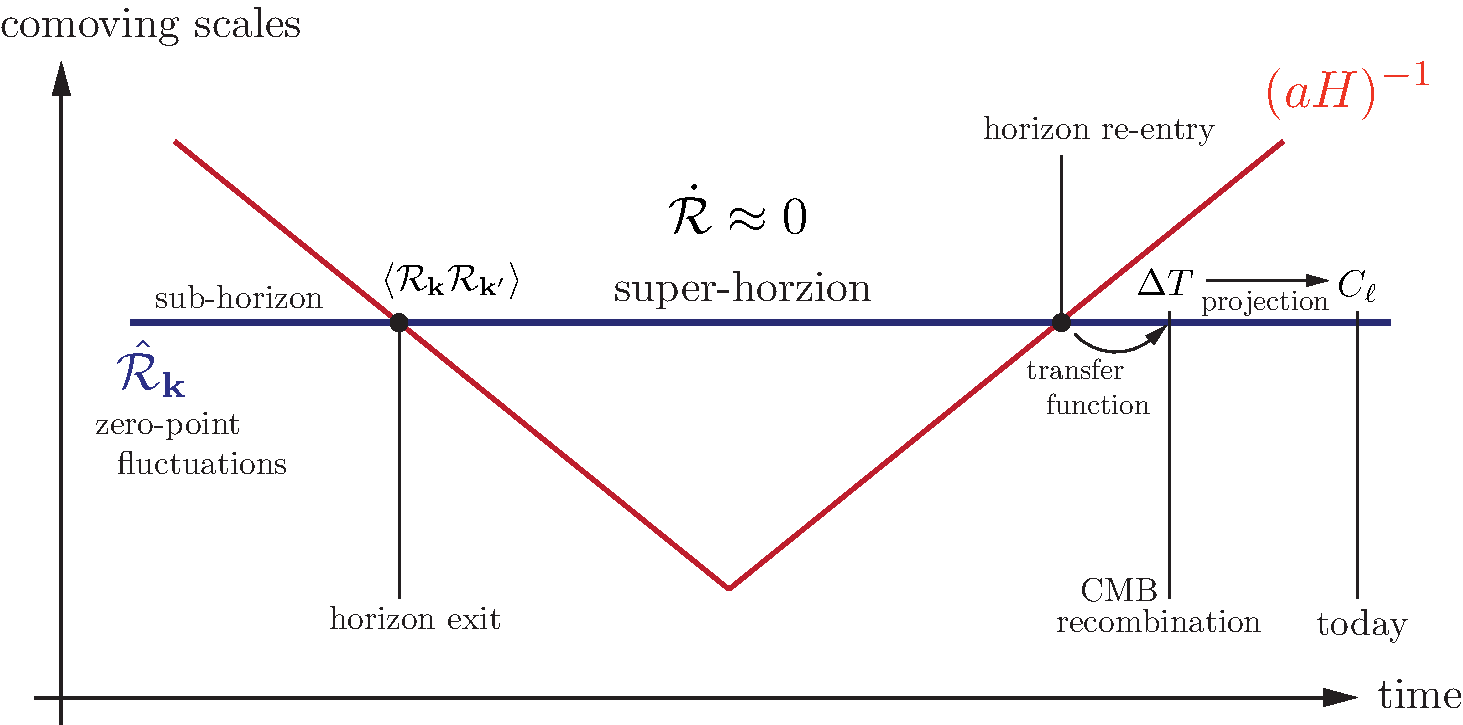
\includegraphics[width=0.75\textwidth]{./summary}
   \caption{\small インフレーション宇宙における摂動の生成と時間発展．揺らぎは地平線内のスケールで量子力学的に生成される（{\bf 第2講}参照）．共動スケール$k^{-1}$が一定に保たれる一方，インフレーション中の共動ハッブル半径$(aH)^{-1}$は縮小するため，摂動は地平線を退出し，後の時代に地平線へ再突入するまで凍結する．地平線再突入後，揺らぎはCMBの異方性とLSSの摂動へ発展する．宇宙論的観測を，インフレーションが刻んだ原始摂動に関係付けるには，この時間発展を考慮しなければならない（{\bf 第3講}参照）．}
    \label{fig:scales3}
\end{figure}

曲率摂動$\R$と重力波の振幅$h$は，モードが地平線を退出すると，$k=a(\tau_\star) H(\tau_\star)$，いずれも一定値で凍結する．
そのため前講では，地平線退出時$\tau_\star$の原始摂動を計算した．
これを宇宙論的観測量（CMB温度や銀河の密度など）に結び付けるには，次が必要である．
\begin{enumerate}
\item[i)] $\R$（または$h$）を，実験で実際に測定される量${\cal Q}$に関係付ける．
\item[ii)] 地平線へ再突入した後の$\R$（および${\cal Q}$）の時間発展を考慮する．
\end{enumerate}
模式的には，次のように書ける．
\beq
\fbox{$\displaystyle
{\cal Q}_{\bf k}(\tau) = T_{\cal Q}(k, \tau,\tau_\star) \, \R_{\bf k}(\tau_\star) $}\, ,
\eeq
ここで，$T_{\cal Q}$は，時刻$\tau_\star$での$\R$の揺らぎと，それより後のある時刻$\tau$での${\cal Q}$の揺らぎを結ぶ{\it 伝達関数}である．
表記からわかるように，伝達関数はスケールに依存しうる．
量${\cal Q}$は，ウィルキンソン・マイクロ波異方性探査機（WMAP）のようなCMB衛星が測定する温度揺らぎであっても，スローン・デジタル・スカイサーベイ（SDSS）のような銀河サーベイから推定する銀河密度であってもよい．


\vskip 6pt
\noindent
{\it CMB異方性}

\S\ref{sec:CMB}の主な結果は，インフレーションの入力スペクトル$P(k) \equiv \{ P_\R(k), P_h(k) \}$と，CMB温度揺らぎおよび偏光の角度パワースペクトルとの次の関係である．
\beq
\label{equ:CXY}
\fbox{$\displaystyle
C_\ell^{XY} = \frac{2}{\pi} \int k^2 \d k \underbrace{P(k)}_{\text{インフレーション}}\,  \underbrace{\Delta_{X \ell}(k) \Delta_{Y \ell}(k)}_{\text{異方性}} $}\, ,
\eeq
ここで，
\beq
\label{equ:source}
\Delta_{X \ell}(k) = \int_0^{\tau_0} \d \tau\, \underbrace{S_X(k, \tau)}_{\text{源}}\, \underbrace{P_{X\ell}(k[\tau_0-\tau])}_{\text{投影}}\, .
\eeq
添字$X,Y$は，温度$T$および偏光モード$E$と$B$を表す（\S\ref{sec:CMB}参照）．
積分(\ref{equ:CXY})は，インフレーションが予言する非一様性$P(k)$を，CMBで観測される異方性$C_\ell^{XY}$に結び付ける．異なる$X$および$Y$モード間の相関は，伝達関数$\Delta_{X\ell}(k)$と$\Delta_{Y\ell}(k)$によって関係付けられる．
伝達関数は，視線方向の積分(\ref{equ:source})として書ける．その被積分関数は，物理的な源の項$S_X(k, \tau)$と幾何学的な投影因子$P_{X\ell}(k[\tau_0-\tau])$（ベッセル関数の組合せ）に因数分解される．
源の項と投影因子の導出は本講の範囲を超えるが，Dodelsonの教科書\cite{Dodelson}にある．これらの結果の直観的な説明は，Wayne Huのウェブサイト\cite{WayneHu}にあるアニメーションで見られる．

本講での関心は，原始パワースペクトル$P_\R(k)$と$P_h(k)$に対する実験的制限にある．
原始スペクトルを測るには，適切な伝達関数と投影効果を考慮して，観測されたCMB異方性$C_{\ell}^{XY}$を{\it デコンボリューション}する必要がある．すなわち，背景宇宙論が与えられれば，式(\ref{equ:CXY})の時間発展と投影の効果を計算し，インフレーションの初期条件$P(k)$を取り出せる．このデコンボリューションの手続きによって，CMBは初期宇宙を探る魅力的な手段となる．

\vskip 6pt
\noindent
{\it 大規模構造}

物質分布の揺らぎ（例えば天球上の銀河分布によって測定される）を調べるため，密度コントラスト$\delta \equiv \delta \rho/ \bar \rho$を定義する．
銀河密度の揺らぎ$\delta_g$と暗黒物質密度の揺らぎ$\delta$は区別する．通常の仮定は，銀河が，その背後にある暗黒物質分布の（バイアスをもつ）トレーサーであるというもので，$\delta_g = b\, \delta$と書く．
{\it バイアス}パラメータ$b$を独立に決める方法があれば，銀河密度コントラスト$\delta_g$の観測から，背後の暗黒物質分布$\delta$を推定できる．
後期の暗黒物質密度揺らぎのパワースペクトルは，曲率揺らぎの原始スペクトルと次のように関係する．
\beq
\fbox{$\displaystyle
P_\delta(k, \tau) = \frac{4}{25} \left( \frac{k}{aH}\right)^4 T_\delta^2(k, \tau) P_\R(k)$}\, .
\eeq
伝達関数からくくり出した数値係数と$k$に関するスケーリングは，慣習によるものである．
伝達関数$T_\delta$は，物質優勢期の揺らぎの成長$\delta \sim a$と，放射優勢期の成長$\delta \sim \ln a$の違いを反映している．
通常，これは{\sf CMBFAST}~\cite{CMBFAST}や{\sf CAMB}~\cite{CAMB}などのコードを用いて数値的に計算する必要があるが，\S\ref{sec:T}では$T_\delta$の便利な近似関数を紹介する．
ここでも，背景宇宙論を固定すれば伝達関数は既知とみなせるので，物質パワースペクトルの観測は，初期宇宙に由来する初期揺らぎを探る手段になる．
%bias: relation between dark matter and galaxies; major uncertainty


\sectionlink{{\sl 復習}：宇宙マイクロ波背景放射}
\label{sec:CMB}


CMB揺らぎの物理と統計的解釈を，ごく簡単に復習する．
さらに詳しい説明は，Dodelsonの教科書\cite{Dodelson}や，{\sl TASI 2009}でのPierpaoli教授の講義にある．


\subsectionlink{温度異方性}

\subsubsection{球面調和関数展開}


 
\begin{figure}[h!]
    \centering
        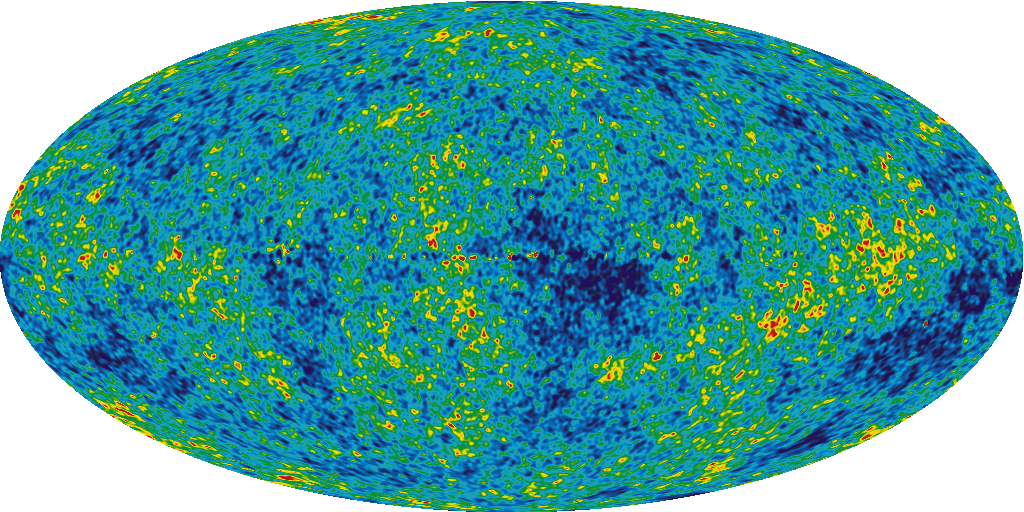
\includegraphics[width=0.7\textwidth]{cmb.png}
    \caption{\small CMBの温度揺らぎ．青い点は，CMB温度が平均値$T_0=2.7$ Kより$\sim 10^{-5}$低い天球上の方向を表す．これは，初期宇宙の高密度領域の重力ポテンシャルを登って脱出する際に，光子がエネルギーを失うことに対応する．黄色と赤は高温（低密度）の領域を表す．これらの揺らぎの統計的性質は，宇宙の背景の時間発展と初期条件の両方について重要な情報を含む．} % (see Figures \ref{fig:WMAP2} and \ref{fig:CMBparam}).}
    \label{fig:WMAP}
\end{figure} 

図\ref{fig:WMAP}は，背景温度$T_0 = 2.7$ Kに対して測定されたCMB温度揺らぎ$\Delta T(\hat n)$の地図を示す．
ここで，単位ベクトル$\hat n$は天球上の方向を表す．
この地図の球面調和関数展開は，
\beq
\label{equ:Tharm}
\Theta(\hat n) \equiv\frac{\Delta T(\hat n)}{T_0}= \sum_{\ell m} a_{\ell m} Y_{\ell m}(\hat n)\, ,
\eeq
ここで，
\beq
a_{\ell m} = \int \d \Omega\, Y^*_{\ell m}(\hat n) \Theta(\hat n)\, .
\eeq
ここで，$Y_{\ell m}(\hat n)$は2次元球面上の標準的な球面調和関数であり，$\ell=0$，$\ell=1$，$\ell=2$はそれぞれ単極子，双極子，四重極子に対応する．
磁気量子数は$m= - \ell, \dots , + \ell$を満たす．
多重極モーメント$a_{\ell m}$を組み合わせると，回転不変な角度パワースペクトルが得られる．% is defined as
\beq
\label{equ:Cl}
C_\ell^{TT} = \frac{1}{2\ell+1} \sum_m  \langle a^*_{\ell m} a_{\ell m} \rangle \, , \qquad \text{または} \qquad  \langle a^*_{\ell m} a_{\ell' m'} \rangle  = C_\ell^{TT} \delta_{\ell \ell'} \delta_{m m'}\, .
\eeq
角度パワースペクトルは，CMBの統計解析における重要な道具である．CMB地図の数百万画素に含まれる宇宙論的情報を，はるかにコンパクトなデータ表現で記述する．図\ref{fig:WMAP2}は，CMB角度パワースペクトルの最新の測定を示す．同図には，CMBスペクトルの理論予言をデータに当てはめた結果も示している．
理論曲線は，背景宇宙論のパラメータと初期揺らぎのスペクトルの両方に依存する．したがって，CMBでその両方を探ることができる．


\begin{figure}[h!]
    \centering
        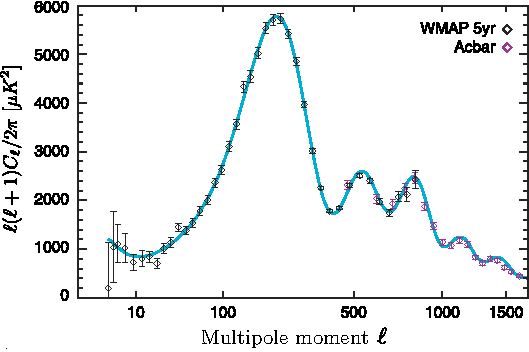
\includegraphics[width=0.65\textwidth]{WMAP_ACBAR}
    \caption{\small CMB温度揺らぎの角度パワースペクトル．} % (see Figures \ref{fig:WMAP2} and \ref{fig:CMBparam}).}
    \label{fig:WMAP2}
\end{figure} 


CMB温度揺らぎは，{\it スカラー}モード$\R$によって支配される（少なくとも，現在考慮されているテンソル・スカラー比$r <0.3$の範囲では）．
$\R$と$\Delta T$を結ぶ線形の時間発展は，伝達関数$\Delta_{T \ell}(k)$を通じ，次の$k$空間積分で与えられる\cite{Dodelson}．
\beq
\label{equ:alm} 
\fbox{$\displaystyle
a_{\ell m} = 4\pi (-i)^\ell \int \frac{\d^3 k}{(2\pi)^3} \, \Delta_{T \ell}(k)\, \R_{\bf k} \, Y_{\ell m}(\hat {\bf k}) $}\, .
\eeq
式(\ref{equ:alm})を(\ref{equ:Cl})に代入し，恒等式
\beq
\sum_{m=-\ell}^\ell Y_{\ell m}(\hat {\bf k}) Y_{\ell m}(\hat {\bf k}') = \frac{2\ell+1}{4\pi} P_\ell(\hat {\bf k} \cdot \hat {\bf k}')\, ,
\eeq
を用いると，
\beq
\label{equ:Cl2}
C_\ell^{TT} = \frac{2}{\pi} \int k^2 \d k \underbrace{P_\R(k) }_{\text{インフレーション}} \underbrace{\Delta_{T \ell}(k) \Delta_{T \ell}(k)}_{\text{異方性}} \, .
\eeq
伝達関数$\Delta_{T\ell}(k)$は一般に，{\sf CMBFAST}~\cite{CMBFAST}や{\sf CAMB}~\cite{CAMB}などのボルツマン計算コードを用いて数値計算する必要がある．これらは背景宇宙論のパラメータに依存する．背景宇宙論を固定すると，パワースペクトル$C_{\ell}^{TT}$の形は，原始パワースペクトル$P_\R(k)$で記述される初期条件についての情報を含む．\footnote{実際には，CMBデータに対して，背景宇宙論と揺らぎのスペクトルを同時に当てはめる．}もちろん，観測から$P_\R(k)$，したがってインフレーションについて学ぶことが，本講の主な目的である．
%where
%\beq
%\Delta_{T \ell}(k) = \int_0^{\tau_0} \d \tau\, \underbrace{S_T(k, \tau)}_{\rm Sources}\, \underbrace{P_{T\ell}(k[\tau_0-\tau])}_{\rm Projection}
%\eeq


\subsubsection{大きなスケール}

大きなスケールのモードは，再結合時にはまだ地平線の外側にあった．
したがって，大スケールのCMBスペクトルは地平線内の時間発展の影響を受けておらず，再結合時の原始スペクトルを現在のわれわれの位置へ幾何学的に投影したものにすぎない．
この{\it ザックス＝ヴォルフェ領域}では，伝達関数$\Delta_{T\ell}(k)$は単なるベッセル関数である\cite{Dodelson}．
\beq
\Delta_{T \ell}(k) = \frac{1}{3} j_\ell(k[\tau_0-\tau_{\rm rec}])\, .
\eeq
したがって，大きなスケール（小さい$\ell$）での角度パワースペクトルは，
\beq
\label{equ:Cl3}
C_\ell^{TT} = \frac{2}{9 \pi} \int k^2 \d k \, P_\R(k) \, j_\ell^2(k[\tau_0-\tau_{\rm rec}]) \, .
\eeq
ベッセル投影関数は$k[\tau_0-\tau_{\rm rec}] \approx \ell$にピークをもち，実質的に$k$と$\ell$を対応付ける$\delta$関数のように作用する．
波数$k\approx \ell/(\tau_0-\tau_{\rm rec})$のモードが式(\ref{equ:Cl3})の積分を支配することから，次のように書ける．
\beq
C_\ell^{TT} \propto \left. k^3 P_\R(k) \right|_{k\approx \ell/(\tau_0-\tau_{\rm rec})} \underbrace{\int \d \ln x \ j^2_\ell(x)}_{\propto\, \ell(\ell+1)}\, .
\eeq
したがって，
\beq
\ell(\ell+1) C_\ell^{TT} \propto \left. \Delta_{\rm s}^2(k) \right|_{k\approx \ell/(\tau_0-\tau_{\rm rec})} \propto \ell^{\, n_{\rm s}-1}\, .
\eeq
入力スペクトルがスケール不変$n_{\rm s} =1$の場合，次の量は，
\beq
{\cal C}_\ell \equiv \frac{\ell(\ell+1)}{2\pi} C_\ell^{TT}
\eeq
$\ell$に依存しない（ただし，暗黒エネルギー優勢の宇宙で重力ポテンシャルが後期に時間発展することで生じる，積分ザックス＝ヴォルフェ効果による非常に小さい$\ell$での増加を除く）．
このため，CMBパワースペクトルは$C_\ell^{TT}$の代わりに${\cal C}_\ell$で描かれることが多い．


\subsubsection{非ガウス性}

ここまで，地平線内の時間発展と幾何学的投影効果を考慮すれば，CMB揺らぎの角度パワースペクトルが実質的に原始パワースペクトル$P_\R(k)$の尺度となることを示した．
\beq
\langle a^*_{\ell m} a_{\ell' m'} \rangle = C_\ell^{TT} \delta_{\ell \ell'} \delta_{m m'} \quad \Leftrightarrow \quad 
\langle \R_{{\bf k}} \R_{{\bf k}'} \rangle = (2\pi)^3 P_\R(k)\, \delta({\bf k} + {\bf k}')\, .
\eeq
原始揺らぎがガウス的なら，$P_\R(k)$がすべての情報を含む．
実際，単一場スローロール・インフレーションは，$\R$が非常に高い精度でガウス的になると予言する\cite{malda}．
しかし，{\bf 第4講}で説明するように，たとえわずかな非ガウス性であっても，最も単純な単一場スローロール模型を超える必要があることを意味するため，インフレーションの作用について重要な情報を与える．

非ガウス性の主な尺度は，{\it 3点関数}，またはそれと等価な{\it バイスペクトル}である．
\beq
 \langle \R_{{\bf k}_1} \R_{{\bf k}_2} \R_{{\bf k}_3}\rangle = (2\pi)^3 B_\R(k_1,k_2,k_3)\, \delta({\bf k}_1 + {\bf k}_2+{\bf k}_3)\, .
\eeq
CMBでは，ゼロでないバイスペクトル$B_\R(k_1, k_2, k_3)$が，角度バイスペクトルに痕跡を残す．
\beq
\label{equ:Bl0}
B^{\ell_1 \ell_2 \ell_3}_{m_1 m_2 m_3} = \langle a_{\ell_1 m_1} a_{\ell_2 m_2} a_{\ell_3 m_3}\rangle \, .\eeq
式(\ref{equ:alm})を(\ref{equ:Bl0})へ代入すると，原始バイスペクトルを，観測されるCMBバイスペクトルに結び付けられる\cite{NGreview}．\footnote{非線形の時間発展は，さらに非ガウス性を生じさせることがある（{\bf 第4講}参照）．}

原始バイスペクトル$B_\R(k_1,k_2,k_3)$は，運動量保存だけを制約とする三つの運動量の関数であることに注意しよう（すなわち，三つのベクトル${\bf k}_i$は閉じた三角形をなす）．
このため，非ガウス性への観測的制限を得るのは難しい（考慮すべき非ガウス性の形が多数ある）．一方，検出されれば，非ガウス性には初期宇宙の物理について多くの情報が含まれるということでもある．

原始非ガウス性の簡単な模型は{\it 局所型非ガウス性}であり，曲率摂動をそのガウス成分$\R_g$の周りでテイラー展開して定義される．
\beq
\label{equ:localx}
\R({\bf x}) = \R_g({\bf x}) + \frac{3}{5} f_{\rm NL}^\R \star \R_g^2({\bf x})\, .
\eeq
これは実空間で局所的であり，パラメータ$f_{\rm NL}^\R$が非ガウス性の大きさを特徴付ける．
式(\ref{equ:localx})から，バイスペクトルについて次の簡単な形が得られることを，読者は確かめてみてほしい．
\beq
B_\R(k_1,k_2,k_3) = \frac{6}{5} f_{\rm NL}^\R \Bigl[ P_\R(k_1) P_\R(k_2) + P_\R(k_2) P_\R(k_3) + P_\R(k_3) P_\R(k_1)\Bigr]\, .
\eeq
したがって，現在の非ガウス性への観測的制限は，パラメータ$f_{\rm NL}^\R$への制限として述べられることが多い（\S\ref{sec:evidence}参照）．

\subsectionlink{偏光}

CMB偏光は，初期宇宙を支配する物理を探る最も重要な手段の一つになると考えられる．
CMBの温度異方性に加え，CMBはトムソン散乱によって偏光すると期待される\cite{Dodelson}．これから説明するように，この偏光には原始揺らぎ，したがってインフレーションについての重要な情報が含まれる\cite{WhitePaper}．

\begin{figure}[htbp!]
    \centering
        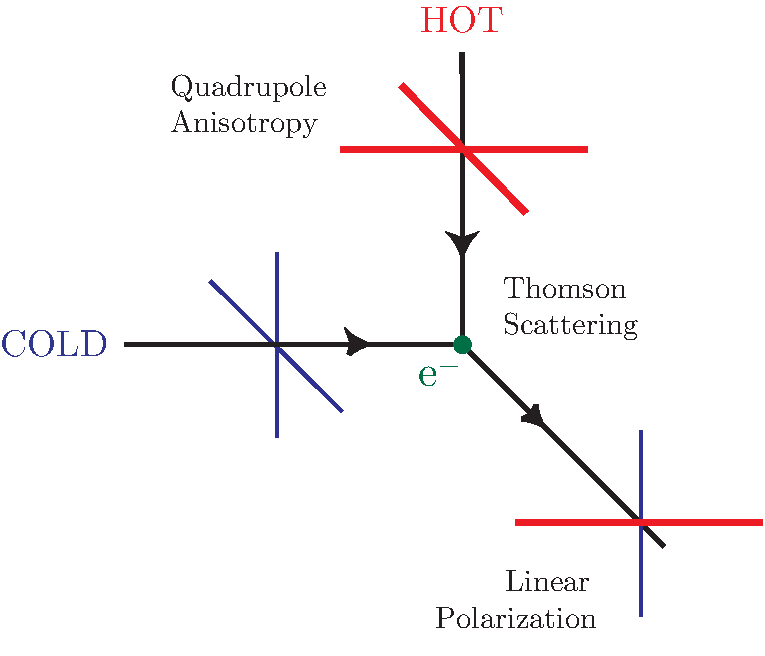
\includegraphics[width=0.55\textwidth]{PolarizationV3}
   \caption{四重極異方性をもつ放射のトムソン散乱によって，直線偏光が生成される．ここで，赤い（太い）線は高温の放射を，青い（細い）線は低温の放射を表す．}
    \label{fig:pol}
\end{figure}

\subsubsection{トムソン散乱による偏光}

%Thomson scattering between electrons and photons produces a simple relationship between temperature anisotropy and polarization.
光子と自由電子の散乱によって偏光がどのように生成されるかを見てみよう．
入射放射の分布が（電子の静止系で）等方的なら，直交する偏光方向が互いに打ち消し合うため，出てくる放射は無偏光のままである．
正味の直線偏光が生じるのは，入射放射場に四重極成分がある場合だけである（図\ref{fig:pol}参照）．
このような四重極モーメントは，再結合の直前に光子が電子や陽子から脱結合するときに生成される．温度異方性は原始密度揺らぎによって作られるので，偏光の一成分は温度異方性と相関するはずである．


\subsubsection{放射場の特徴付け}

%We digress briefly to give details of the mathematical characterization of CMB temperature and polarization anisotropies.
CMB偏光異方性の数学的な特徴付けは，温度揺らぎの記述より少し複雑である．偏光はスカラー場ではないため，通常の球面調和関数による展開が適用できないからである．

異方性の場は，$2\times 2$の強度テンソル$I_{ij}(\hat n)$で定義される．ここで，これまでと同様に$\hat n$は天球上の方向を表す．$I_{ij}$の成分は，$\hat n$に垂直な二つの直交基底ベクトル$\hat{\bf e}_1$と$\hat {\bf e}_2$に対して定義される．
直線偏光はストークスパラメータ$Q = \frac{1}{4}(I_{11}-I_{22})$と$U=\frac{1}{2} I_{12}$で記述され，温度異方性は$T = \frac{1}{4} (I_{11}+I_{22})$である．
偏光の大きさと角度は，それぞれ$P =\sqrt{Q^2 +U^2}$と$\alpha = \frac{1}{2} \tan^{-1}(U/Q)$である．
量$T$は$\hat n$に垂直な平面内での回転に不変なので，スカラー（スピン0）の球面調和関数(\ref{equ:Tharm})で展開できる．
%\beq
%T(\hat n) = \sum_{\ell, m}  a_{\ell m}^T\ Y_{\ell m}(\hat n)\, .
%\eeq
一方，量$Q$と$U$は，角度$\psi$の回転の下でスピン2の場として変換し，$(Q \pm iU)(\hat n) \to e^{\mp 2 i \psi} (Q \pm i U)(\hat n)$となる．したがって，$Q \pm i U$の調和解析には，テンソル（スピン2）の球面調和関数による球面上の展開が必要である\cite{Kamionkowski:1996ks, Zaldarriaga:1996xe, NewmanPenrose}．
\beq
(Q \pm iU)(\hat n) = \sum_{\ell, m}  a_{\pm 2,\ell m} \, {}_{\pm 2}Y_{\ell m}(\hat n)\, .
\eeq
これらのテンソル球面調和関数${}_{\pm 2}Y_{\ell m}$の数学的性質を説明すると，本講の主題から外れすぎるので，古典的な論文\cite{Kamionkowski:1996ks, Zaldarriaga:1996xe}やDodelsonの教科書\cite{Dodelson}を参照してほしい．

\subsubsection{$E$モードと$B$モード}
モーメント$a_{\pm2,\ell m}$の代わりに，次の線形結合を導入すると便利である．%\cite{NewmanPenrose}
\beq
a_{E, \ell m} \equiv -\frac{1}{2} \left(a_{2, \ell m} + a_{-2, \ell m}\right)\, , \qquad
a_{B, \ell m} \equiv - \frac{1}{2i} \left(a_{2, \ell m} - a_{-2, \ell m}\right)\, .
\eeq
すると，スピン2の量$Q$と$U$の代わりに，二つのスカラー（スピン0）の場を定義できる．
\beq
E(\hat n) = \sum_{\ell, m} a_{E, \ell m}\, Y_{\ell m}(\hat n)\, , \qquad B (\hat n)=\sum_{\ell, m} a_{B, \ell m}\, Y_{\ell m}(\hat n)\, .
\eeq

\begin{figure}[htbp!]
    \centering
        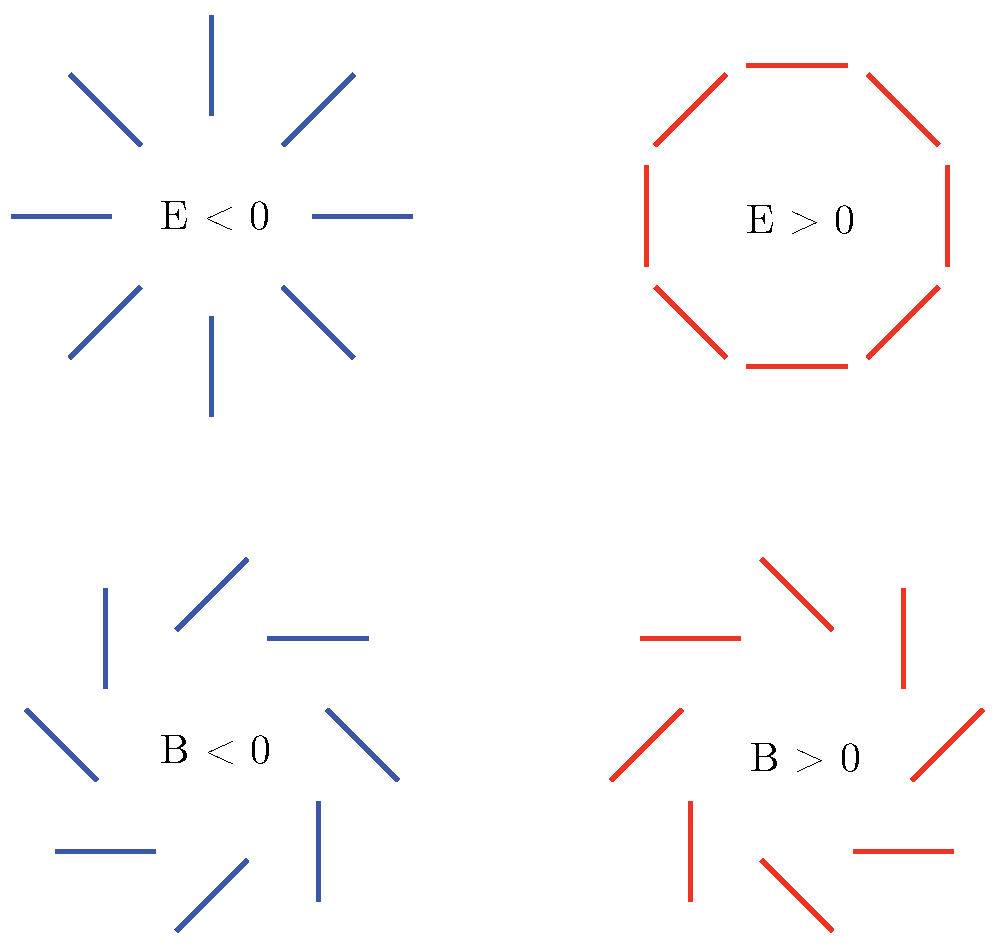
\includegraphics[width=.45\textwidth]{EBmode}
   \caption{偏光の$E$モードと$B$モードのパターンの例．中心を通る直線に関して反転すると，$E$モードのパターンは変わらない一方，正と負の$B$モードのパターンは入れ替わることに注意しよう．}
    \label{fig:EBmode}
\end{figure}

スカラー量$E$と$B$は，直線偏光の場を完全に指定する．
$E$モード偏光は，天球上の低温点の周りで偏光ベクトルが放射状となり，高温点の周りでは接線方向となる，{\it 回転のない}モードとしても特徴付けられる．
一方，$B$モード偏光は{\it 発散がない}が{\it 回転をもつ}．その偏光ベクトルは，天球上の各点の周りに渦度をもつ．\footnote{$E$と$B$という名称は明らかに，静電磁場でおなじみの性質$\nabla \times {\bf E} = 0$と$\nabla \cdot {\bf B} = 0$を反映している．}
図\ref{fig:EBmode}に，$E$モードと$B$モードのパターンの例を示す．
$E$と$B$はいずれも回転に不変だが，パリティ変換の下では異なる振る舞いをする．%$E$-polarization remains unchanged and $B$-polarization changes sign.
中心を通る直線に関して反転したとき，$E$モードのパターンは変わらないが，$B$モードのパターンは符号を変えることに注意しよう．

温度と偏光（$E$モードおよび$B$モード）の異方性の対称性は，4種類の相関を許す．すなわち，温度揺らぎ，$E$モード，$B$モードの自己相関で，それぞれ$TT$，$EE$，$BB$と表されるもの，および温度揺らぎと$E$モードとの相互相関$TE$である．それ以外の相関（$TB$と$EB$）は，対称性のためにすべて消える．
%\footnote{This assumes no parity-violating processes in the early universe.  Conversely, non-zero $TB$ and $EB$ correlations would be a distinctive signature  of such physics.}
  % All these statements apply to primary anisotropies
  %only; at the level of secondary anisotropies, non-zero $TB$ and $EB$-correlations are generated by weak lensing effects.}

角度パワースペクトルは，これまでと同様に定義する．
\beq
C_\ell^{XY} \equiv \frac{1}{2\ell + 1} \sum_m \langle a_{X,\ell m}^* a_{Y,\ell m} \rangle \, , \qquad X, Y = T, E, B\, .
\eeq
図\ref{fig:TE}には，$TE$相互相関の最新の測定\cite{WMAP5}を示す．$EE$スペクトルの測定も始まっているが，誤差はまだ大きい．これまでのところ，$BB$スペクトルについては上限しか得られておらず，検出には至っていない．

\begin{figure}[htbp!]
    \centering
        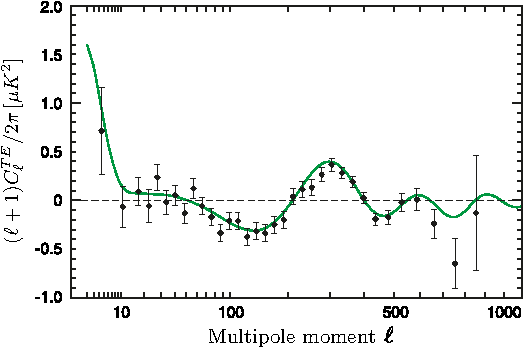
\includegraphics[width=.65\textwidth]{TEv2}
   \caption{温度異方性と$E$モード偏光異方性の相互相関のパワースペクトル\cite{WMAP5}．$\ell = 50-200$（角距離$5^\circ > \theta > 1^\circ$に対応）での反相関は，脱結合期の地平線より大きなスケールにおける断熱揺らぎの特徴的な徴候であり\cite{spergel/zaldarriaga:1997, Dodelson:2003ip}，インフレーションの枠組みの基本的な予言を裏付ける．}
    \label{fig:TE}
\end{figure}

CMB偏光の$E$/$B$分解の宇宙論的な重要性は，文献\cite{Kamionkowski:1996ks, Zaldarriaga:1996xe}の著者らによって認識された．彼らは次の注目すべき事実を証明した．
\begin{enumerate}
\item[i)] スカラー（密度）摂動は$E$モードだけを生成し，$B$モードを{\it 生成しない}．
\item[ii)] ベクトル（渦度）摂動は主として$B$モードを生成する．\footnote{しかし，ベクトルは宇宙の膨張とともに減衰するので，再結合時には劣勢だと考えられている．したがって，ここでは考慮しない．}
%, but note that cosmic strings can produce a $B$-mode signal via vector modes (see \S\ref{sec:defects}).}
\item[iii)] テンソル（重力波）摂動は$E$モードと$B$モードの両方を生成する．
\end{enumerate}
%Intuitively these results may be understood as follows:
%Thomson scattering produces an $E$-mode locally at the scattering event.
%For scalar perturbations the spatial pattern of the polarization field at the last-scattering surface is curl-free. Since free streaming (to linear order) projects a curl-free spatial pattern to a curl-free angular distribution, the observed signal from scalar perturbations remains curl-free and hence pure $E$-mode.
%For tensor modes the polarization is also $E$-mode at last scattering, but the spatial distribution has non-zero curl. Projection of the polarization pattern from the last-scattering surface to the point of observation today therefore produces $B$-mode polarization.

{\it スカラーは$B$モードを生成しない}が，{\it テンソルは生成する}という事実が，$B$モードの検出はテンソルモード，したがってインフレーションの決定的証拠であるという主張の根拠となる．
%The search for the primordial  $B$-mode signature of inflation is often considered the ``holy grail" of observational cosmology.
%We discuss the theoretical implications of the $B$-mode amplitude in Section~\ref{sec:Bmodes}.


\subsubsection{$E$モードとスカラー}

$E$モードのパワースペクトルと$TE$相互相関は，インフレーションの{\it スカラー}モードによって支配される．すなわち，
\bea
C_\ell^{EE} &\approx& (4\pi)^2 \int k^2 \d k \overbrace{P_\R(k) }^{\text{インフレーション}} \Delta_{E \ell}^2(k) \, ,\\
%\underbrace{\Delta_{B \ell}(k) \Delta_{B \ell}(k)}_{\rm Anisotropies} 
C_\ell^{TE} &\approx& (4\pi)^2 \int k^2 \d k \underbrace{P_\R(k) }_{\text{インフレーション}} \Delta_{T\ell}(k) \Delta_{E \ell}(k)\, .
%\underbrace{\Delta_{B \ell}(k) \Delta_{B \ell}(k)}_{\rm Anisotropies} 
\eea
$C_\ell^{TT}$と同様に，スペクトル$C_\ell^{EE}$と$C_\ell^{TE}$は$P_\R(k)$についての情報を与える．
しかし，それぞれの場合で原始スペクトルは異なる伝達関数と畳み込まれるため（偏光は自由電子による散乱だけで生成される），これらの信号は有用な相補性をもつ．

\subsubsection{$B$モードとテンソル}

$B$モードは{\it テンソル}モードだけによって生成される．すなわち，
\beq
C_\ell^{BB} = (4\pi)^2 \int k^2 \d k \underbrace{P_h(k) }_{\text{インフレーション}} \Delta_{B \ell}^2(k)\, .
%\underbrace{\Delta_{B \ell}(k) \Delta_{B \ell}(k)}_{\rm Anisotropies} 
\eeq
%where
%\beq
%\Delta_{B \ell}(k) = \int_0^{\tau_0} \d \tau\, \underbrace{S_B(k, \tau)}_{\rm Sources}\, \underbrace{P_{B\ell}(k[\tau_0-\tau])}_{\rm Projection}
%\eeq
したがって，$C_\ell^{BB}$の測定は，原始テンソル揺らぎの情報を得る独自の機会となる．

\begin{figure}[h!]
    \centering
        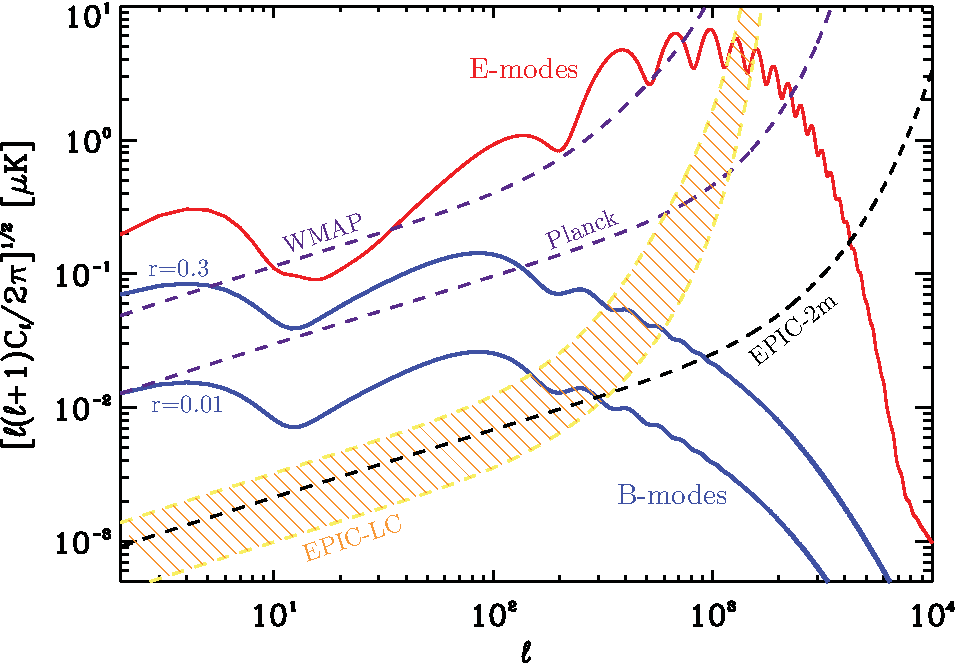
\includegraphics[width=0.65\textwidth]{EPIC}
    \caption{現在の上限に等しいテンソル・スカラー比$r=0.3$，および$r=0.01$に対する$E$モードと$B$モードのパワースペクトル．{\sl WMAP}，{\sl Planck}，および将来のCMB衛星（{\sl CMBPol}）の二つの異なる設計案（EPIC-LCとEPIC-2m）の実験感度も示している\cite{EPIC}．}
    %({\small Figure adapted from Bock {\it et al.}~\cite{EPIC}.})}
    \label{fig:spectra}
\end{figure}


\sectionlink{{\sl 復習}：大規模構造}

\begin{figure}[h!]
    \centering
        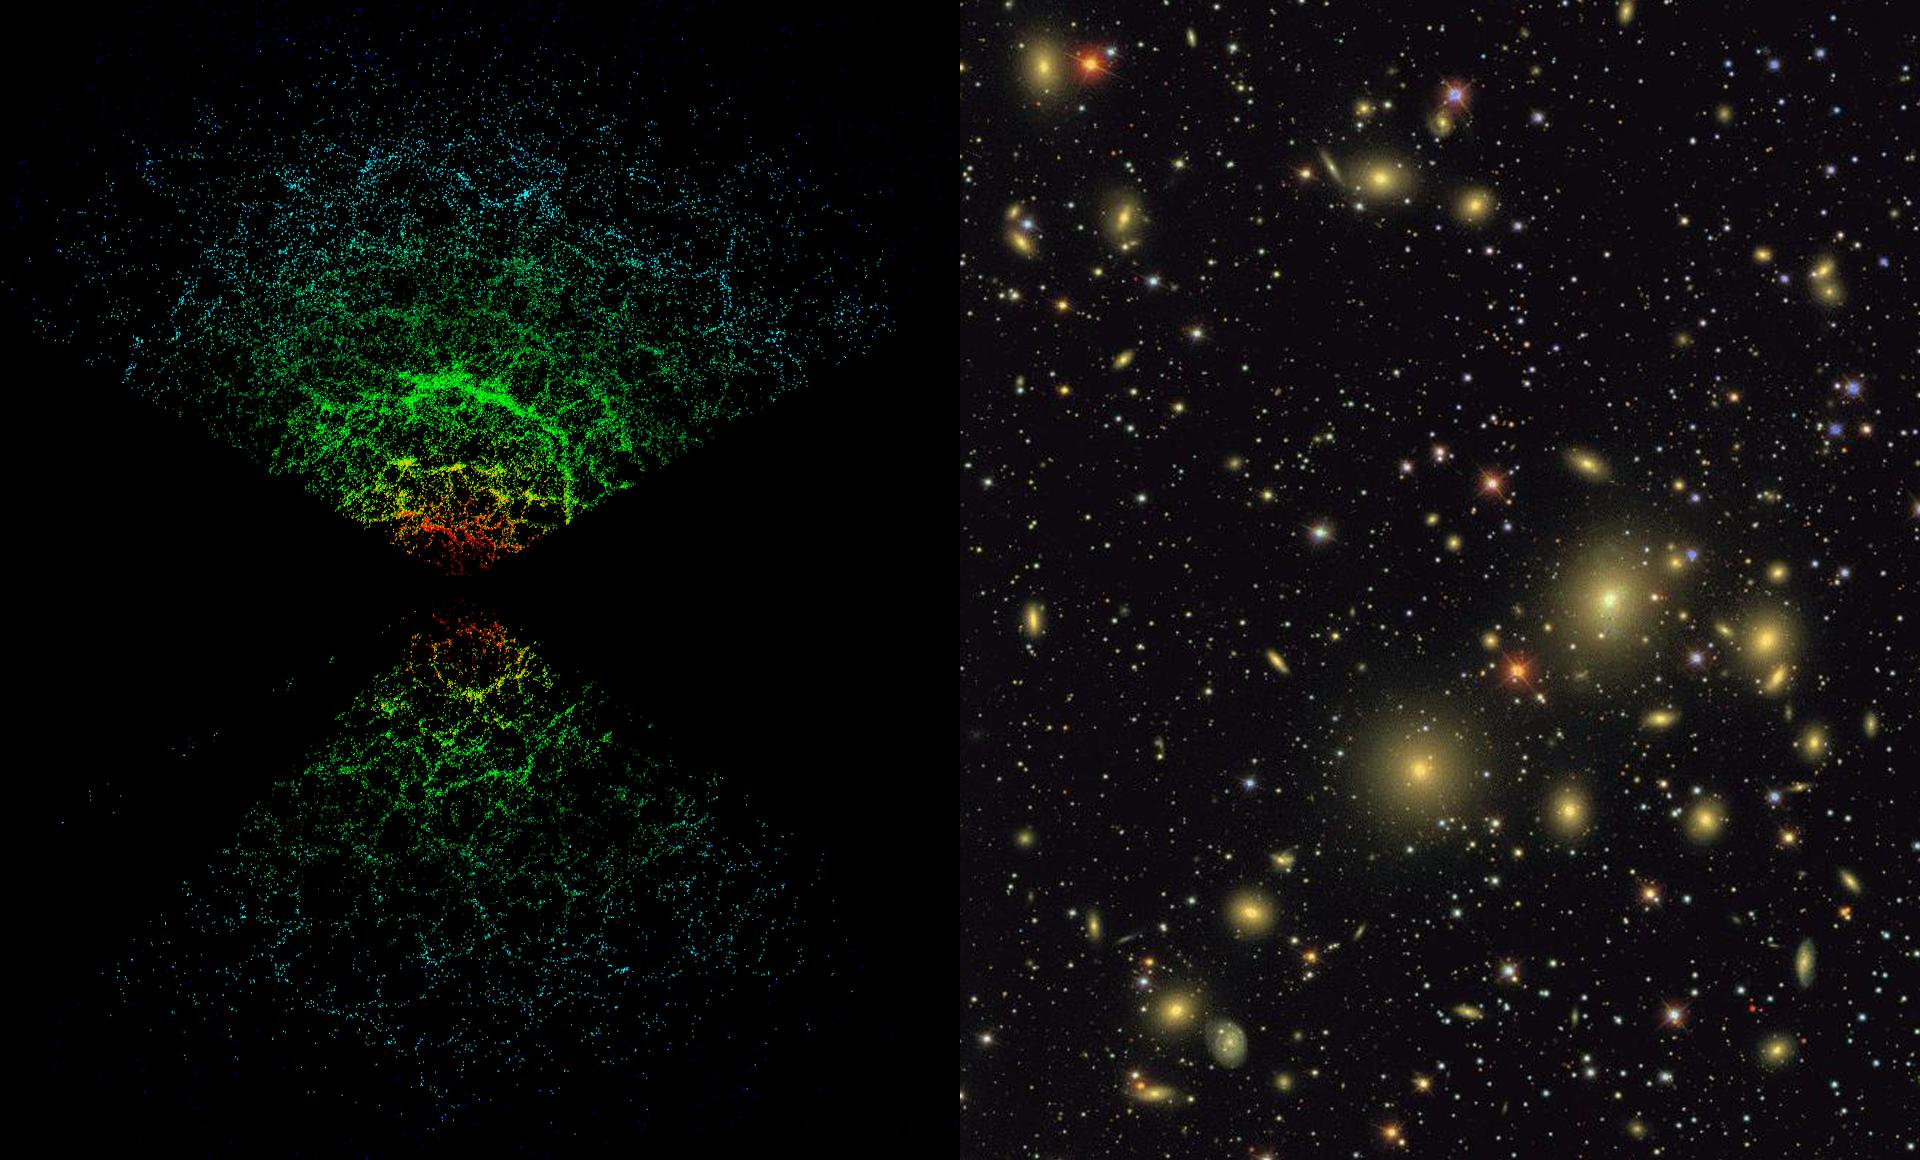
\includegraphics[width=.9\textwidth]{galaxies.jpg}
    \caption{\small 銀河の分布．スローン・デジタル・スカイサーベイ（SDSS）は，約100万個の銀河の位置と距離（赤方偏移）を測定した．
    まず右上のような2次元画像で同定した銀河について，距離を測定して3次元地図を作る．左の画像は，そのような3次元地図の一断面を示す．測定された銀河分布の統計的性質は，後期宇宙の構造と進化について重要な情報を明らかにする．}
    \label{fig:SDSS}
\end{figure}

銀河（または暗黒物質）のパワースペクトルは，原始曲率揺らぎのスペクトルの尺度となる．
\beq
P_\delta(k, z) \quad \Rightarrow \quad P_\R(k)\, ,
\eeq
ただし，地平線内の時間発展の効果を考慮する必要がある．
これは，暗黒物質の伝達関数によって行う．

\subsectionlink{暗黒物質の伝達関数}
\label{sec:T}


密度揺らぎは，圧力と重力の競合の下で時間発展する．
放射優勢期には，強い放射圧が揺らぎの急速な成長を妨げるため，密度コントラストは対数的にしか成長せず，$\delta \sim \ln a$となる．
物質優勢期には，背景の圧力が無視でき，重力収縮がより効果的に働くため，$\delta \sim a$となる．

地平線突入から物質優勢期までの間に摂動が有意には成長しないという簡単化の仮定の下では，次の近似的な伝達関数を導ける．
\beq
\label{equ:Tapprox}
T_\delta(k) \approx \left\{ \begin{array}{l l} 1 & k < k_{\rm eq} \\ (k_{\rm eq}/k)^2 & k > k_{\rm eq} \end{array} \right. \, .
\eeq
式(\ref{equ:Tapprox})は，スペクトルの定性的な形（すなわち$k \approx k_{\rm eq}$でのスペクトルの折れ曲がり）を直観的に理解するには有用だが，ほとんどの応用に対して精度が足りない．
物質の伝達関数に対する有名な近似関数は，Bardeenら（BBKS）\cite{BBKS}によって与えられた．
\beq
T_\delta(q) = \frac{\ln(1+2.34 q)}{2.34 q} \left[ 1+ 3.89 q +(1.61 q)^2 +(5.46 q)^3 + (6.71 q)^4\right]^{-1/4}\, ,
\eeq
ここで，$q=k/\Gamma h\, {\rm Mpc}^{-1}$であり，形状パラメータを次のように定義した．
\beq
\Gamma \equiv \Omega h \exp (-\Omega_b - \sqrt{2h} \Omega_b/\Omega)\, .
\eeq
より正確な伝達関数は，EisensteinとHu\cite{EisensteinHu}にある．
最後に，厳密な伝達関数は{\sf CMBFAST}~\cite{CMBFAST}または{\sf CAMB}~\cite{CAMB}で数値計算できる．

われわれの目的にとって重要なのは，（背景宇宙論のパラメータが与えられれば）暗黒物質の伝達関数を計算でき，それを用いて暗黒物質パワースペクトル$P_\delta(k,z)$をインフレーションのスペクトル$P_{\cal R}(k)$に関係付けられる，という点だけである．

\subsectionlink{銀河バイアス}

残念ながら，重力レンズを除けば暗黒物質を直接観測できない．
（例えばスローン・デジタル・スカイサーベイ（SDSS）のような銀河サーベイで）観測するのは，光を放つ物質，すなわちバリオン物質である．
大きなスケールでは，銀河分布と暗黒物質を結び付ける次の現象論的な仮定が有用であることがわかっている．
\beq
\delta_g = b\, \delta\, ,
\eeq
あるいは，
\beq
P_{\delta_g} = b^2 P_\delta\, .
\eeq
ここで，$b$は（線形）バイアスパラメータと呼ばれる．これは，十分に理解されていない銀河形成の物理を記述するパラメータとみなせる．
バイアスパラメータ$b$は，銀河のバイスペクトル$B_{\delta_g}$を測定して求められる．

こうした複雑さを別にすれば，銀河パワースペクトル$P_{\delta_g}(k)$は，インフレーションのスカラー揺らぎ$P_\R(k)$を探る追加の手段となる．より小さなスケールを調べるため，CMB揺らぎの観測と相補的である．

%\newpage
\sectionlink{インフレーションを支持する現在の証拠}
\label{sec:evidence}

インフレーションは仮説である．
インフレーションが初期宇宙の物理的実在を記述しているという確信を高めるため，その予言を宇宙論的観測と比較する．
本節では，インフレーションを支持する現在の観測的証拠を説明し，次節で将来の検証を論じる．


\subsectionlink{平坦性}

宇宙は，バリオン，暗黒物質，光子，ニュートリノ，暗黒エネルギーで満たされている．
\beq
\Omega_{\rm tot} = \Omega_b + \Omega_{\rm cdm} + \Omega_\gamma + \Omega_\nu + \Omega_\Lambda\, .
\eeq
$\Omega_{\rm tot}$の値は宇宙の空間幾何を決め，$\Omega_{\rm tot}=1$は平坦な宇宙，$\Omega_{\rm tot} < 1$は負の曲率をもつ宇宙，$\Omega_{\rm tot} > 1$は正の曲率をもつ宇宙に対応する．
インフレーションの予言は，
\beq
\Omega_{\rm tot} = 1 \pm 10^{-5}\, ,
\eeq
一方，データは次を示す\cite{WMAP5}．
\beq
\Omega_{\rm tot} = 1 \pm 0.02\, .
\eeq
この理論とデータの一致は見事だが，インフレーションは宇宙の平坦性を，ある意味「設計どおり」に実現しているとも言える．\footnote{ただし，グースが1980年にインフレーションを導入した時点では，宇宙の平坦性は非自明な予言であり，当時の観測と矛盾していたことは指摘しておく価値がある！}
したがって，インフレーションという考え方の追加の検証を探すべきである．


\subsectionlink{位相のコヒーレンスと地平線外の揺らぎ}

本講義で繰り返し強調してきたように，非一様な宇宙の観測によって，インフレーションの力学を詳しく検証できる．
この小節では，インフレーションが自然に説明する，観測の非自明な定性的特徴を論じ，次の小節で定量的な結果を示す．

%\vskip 6pt
以下は，Dodelsonが文献\cite{Dodelson:2003ip}で美しく説明した議論を単純化したものである．

\subsubsection{TTスペクトルのピーク}

インフレーションは，ほぼスケール不変な摂動スペクトルを生成する．
\beq
\langle \R_{\bf k} \R_{\bf k'} \rangle = (2\pi)^3 \delta ({\bf k} +{\bf k}') P_\R(k)\, ,
\eeq
ここで，$k^3 P_\R(k) \propto k^{n_{\rm s}-1}$であり，$n_{\rm s} \approx 1$である．
\begin{quote}
そうすると，パワースペクトルの形を観測で測定でき，それによってインフレーションの正しさを確信するのだと思うかもしれない．確かに，物質と放射の両方についてパワースペクトルを測定でき，観測が理論と一致するのも確かである．しかし，データを見て背筋が震えるのはそのためではない．インフレーション中に生成された摂動の真に驚くべき特徴は，むしろ，{\it すべてのフーリエモードが同じ位相をもつ}ことである\cite{Dodelson:2003ip}．
\end{quote}
物理的波長$\lambda$のフーリエモードを考えよう．インフレーション中に地平線の内側にある間，モードは$k = 2\pi/\lambda$で与えられる振動数で振動する．しかし，インフレーションが終わる前に，モードは地平線を退出する．すなわち，その物理的波長が，その時点のハッブル半径より長く引き伸ばされ，$\lambda > H^{-1}$となる．その後，振幅は一定に保たれる．ずっと後にモードが地平線へ再突入して初めて，因果的な物理過程が作用し，時間発展を起こせるようになる．
揺らぎの振幅は地平線の外側で一定だったので，地平線再突入時の$\dot \R$は非常に小さい．
一般には，各フーリエモードは正弦モードと余弦モードの線形結合でありうる．しかし，インフレーションの特別な点は，余弦モードだけを励起することである（地平線再突入時を$t \equiv 0$と定義する）．

地平線の内側に入ると，曲率摂動$\R$は密度揺らぎ$\delta$の源となり，密度揺らぎは重力と圧力の影響の下で時間発展する．
\beq
\ddot \delta - c_s^2 \nabla^2 \delta = F_g[\R]\, ,
\eeq
ここで，$c_s$は音速，$F_g$は重力の源の項である．
これにより密度場に振動が生じる．初期宇宙のプラズマでは，物質密度の揺らぎは放射の揺らぎと強く結合していた．したがって，CMB揺らぎは，再結合時の背後にある密度場の状態を直接写したスナップショットを与える．
再結合が瞬間的に起こると想像しよう（これはそれほど悪い近似ではない）．
波長の異なる揺らぎは，それぞれの振動の異なる位相で捉えられるだろう．
ある波長のモードは振幅が最大または最小の時点で捉えられ，別の波長のモードは振幅がゼロの時点で捉えられる．
ある波長をもつすべてのフーリエモードの位相が揃っていれば，それらはコヒーレントに干渉し，全フーリエモードのスペクトルは，最終散乱面に見えるCMBパワースペクトルに一連の山と谷を生む．
これはもちろん，図\ref{fig:WMAP}で見ているものである．しかし，初期揺らぎの理論がこれを説明するには，すべてのフーリエモードにコヒーレントな初期位相を生む機構が必要である．インフレーションはまさにそれを行う！
揺らぎは地平線を退出すると凍結するため，フーリエモードの位相は，関心のあるモードが地平線へ入るよりもずっと前に定まっていた．CMBパワースペクトルのピーク構造に感嘆するとき，実際に感嘆しているのは，原始揺らぎを生む機構が，すべてのフーリエモードの位相を揃える能力である．このコヒーレンスがなければ，CMBパワースペクトルは山も谷もない単なる白色雑音となる（実際，宇宙ひもや位相的欠陥が原始揺らぎの主な源として排除されるのは，まさにこの理由である）．

\begin{figure}[h!]
    \centering
        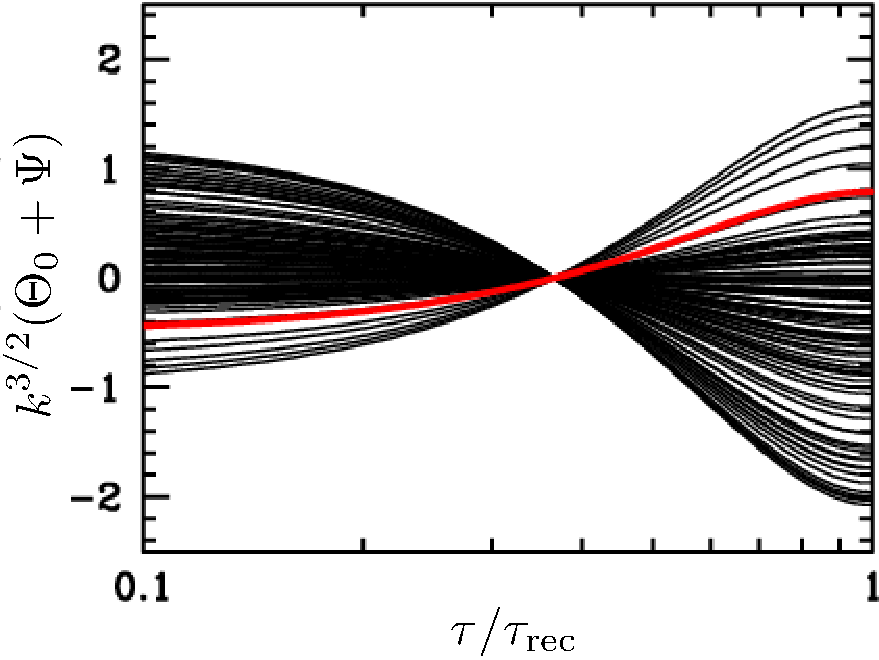
\includegraphics[width=.45\textwidth]{manymodes}
        \hspace{0.2cm}
                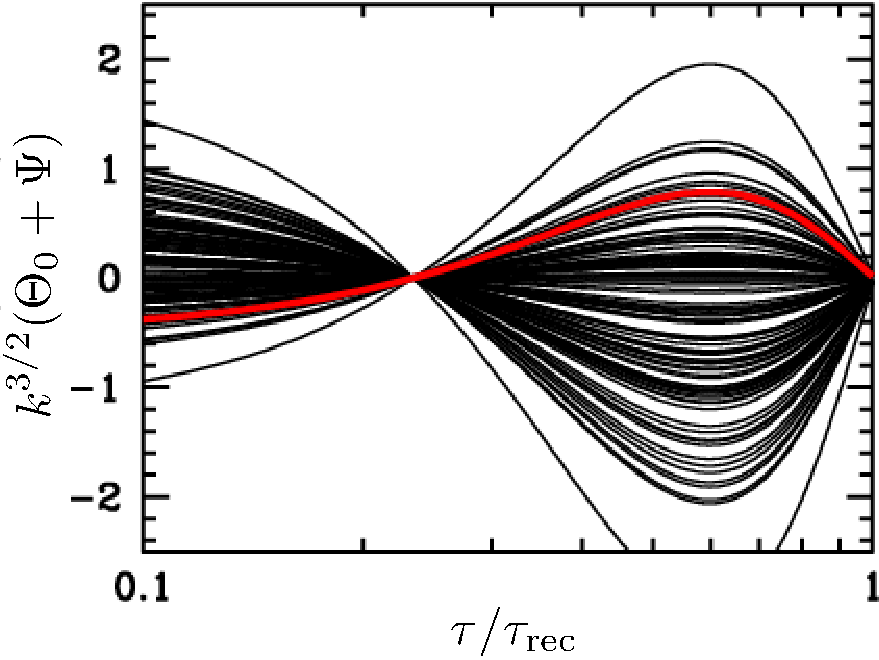
\includegraphics[width=.45\textwidth]{manytrough}
    \caption{\small 同じ波長をもつモードの時間発展．再結合は$\tau = \tau_{\rm rec}$で起こる．左図はCMB角度パワースペクトルの第1ピークに対応する波長を，右図は最初の谷に対応する波長を示す．すべてのモードは同じ位相から出発するため，左のモードはすべて再結合時に最大振幅となり，右のモードはすべて再結合時にゼロになる．これがCMBパワースペクトルのピークを説明する．}
    \label{fig:manymodes}
\end{figure}

\begin{figure}[h!]
    \centering
       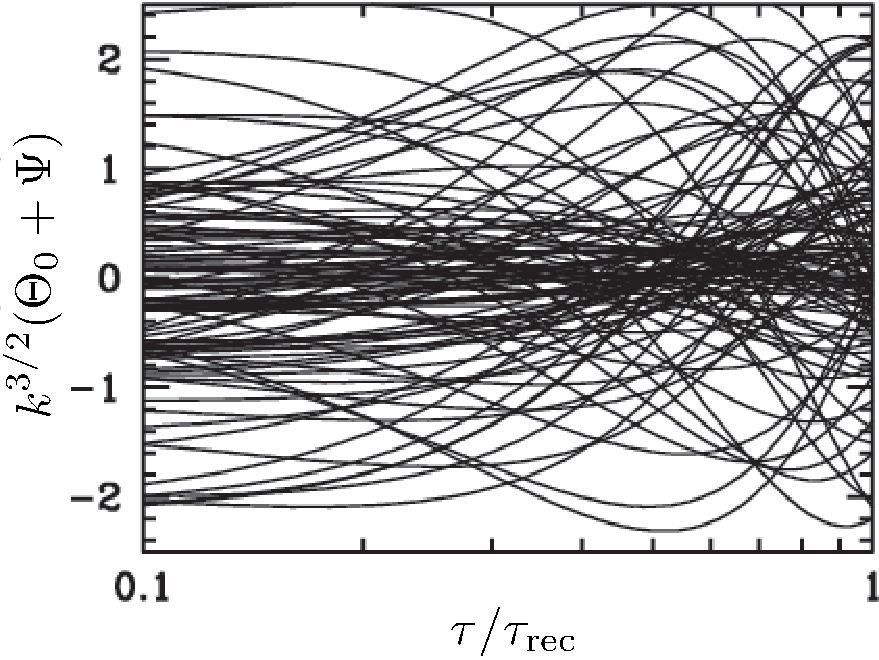
\includegraphics[width=.45\textwidth]{dec1}
         \hspace{0.2cm}
        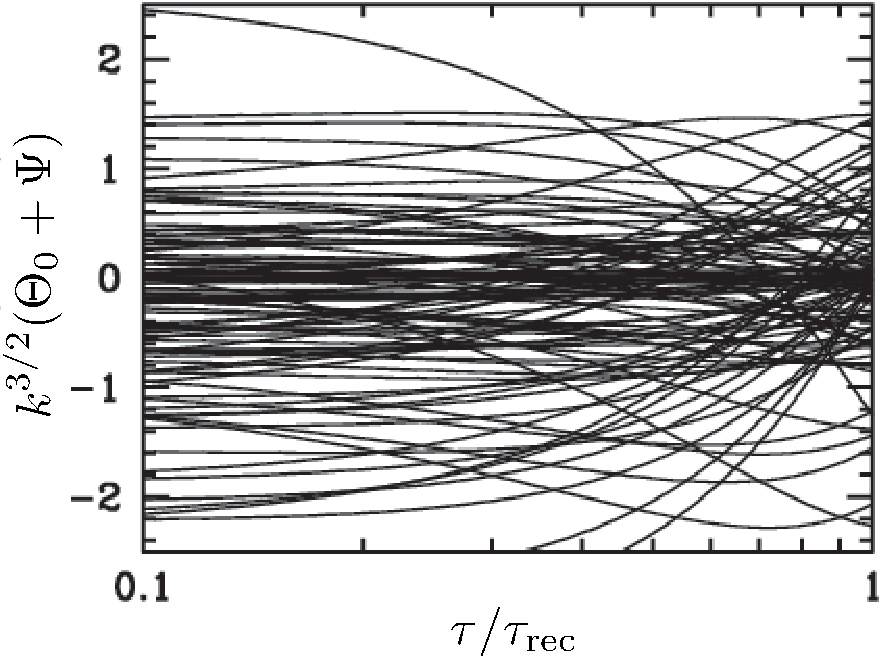
\includegraphics[width=.45\textwidth]{decoher}
    \caption{\small 図\ref{fig:manymodes}と同じ二つの波長に対応するモード．ただし，今度は初期位相がランダムである．CMBの角度方向のピーク構造が消えてしまうことがわかる．}
    \label{fig:decoher}
\end{figure}



\subsubsection{TEスペクトルの$\ell < 100$}

懐疑的な人は，上の議論だけでは納得しないかもしれない．CMB温度揺らぎスペクトルの山と谷は，角度スケール$\theta < 1^\circ$に対応する$\ell >200$にある．これらのスケールはすべて，再結合時には地平線の内側にあった．したがって，因果律に従いながらも「余弦モード」だけを生成する構造形成理論を組み立てることは，原理的には可能である（1990年代には実際に試みられた）．そのような理論は，インフレーションに頼らずにCMBのピークを説明する．最も美しい考え方とは言い難いが，論理的な可能性としては排除できない．

しかし，CMB偏光を考えると，このように高度に調整したインフレーションの代替理論さえも排除できることを，ここで示す．
図\ref{fig:TE}を見ると，CMB温度揺らぎと$E$モード偏光の相互相関は，$100 < \ell < 200$付近に負のピークをもつ．この反相関信号も位相のコヒーレンスの結果だが，今度のスケールは再結合時には地平線の内側に{\it なかった}．したがって，この信号を生成できる（$\tau =0$以降の）因果的な機構は{\it 存在しない}．共動地平線の縮小によって地平線からの退出と再突入が起こる，インフレーションのようなものを考えざるをえない．\footnote{ここで，共動ハッブル半径$1/(aH)$を縮小させる方法が二つあることを述べておく．インフレーション中は$H$がほぼ一定で，スケール因子$a$が指数関数的に成長する．しかし，{\it 収縮する}時空でも，$H$が時間とともに増大すれば地平線を縮小できる．これがエクピロティック／循環宇宙論\cite{Steinhardt:2002ih, Steinhardt:2001st, Buchbinder:2007ad}で用いられる機構である．共動ハッブルスケールの時間発展で見ると，インフレーションとエクピロティック模型は非常によく似ているが，重要な違いがある．例えば，エクピロティック模型では，収縮期を通常のビッグバン膨張に接続することが課題となる．}

Dodelsonは次のように説明している\cite{Dodelson:2003ip}．
\begin{quote}
再結合時には，［密度場の単極子（$T$の源）と双極子（$E$の源）の位相差によって］，両者の積は$100< \ell < 200$で負となり，より小さなスケールでは$\ell \sim 400$まで正となる．しかし，これはまさにWMAPが観測したものである！ 単極子と双極子が再結合時に互いに位相をずらしていたことの明確な証拠がある．

この証拠は，小スケールのモード（$\ell > 200$）についても刺激的である．音響ピークが位相のコヒーレンスを示すのと同様に，偏光と温度の相互相関は，双極子のコヒーレンスも物語っている．これは再結合時のプラズマについてのわれわれの描像を確かなものにする．
しかし，より大きなスケールのモード（$\ell < 200$）からの証拠は，まさに驚異的である．これらのモードは，再結合時には地平線の内側になかったからである．したがって，位相が揃いうる{\it 唯一}の方法は，因果的に接触していた時代に，何らかの原始的な機構がその仕事をしたというものである．インフレーションは，まさにそのような機構である．
\end{quote}

%TE spectrum proves that fluctuations are superhorizon at recombination.

\subsectionlink{スケール不変性，ガウス性，断熱性}
\label{sec:obs:source-duplicate-1}

次に，原始揺らぎに対する定量的な制限を説明する．
最も単純なインフレーション模型は，スカラー摂動がほぼ{\it スケール不変}，{\it ガウス的}，{\it 断熱的}であると予言する．本節では，理論のこれらの基本的な予言に対する最新の定量的制限を示す．

%Inflation predicts correlations of scalar modes $\R$ and tensor modes $h$.If the perturbations are gaussian, the correlations are completely determined by the power spectra $P_\R(k)$ and $P_h(k)$.

\vspace{0.5cm}
\begin{table}[h!]
\begin{center}
\begin{tabular}{||c|c|c||}
\hline \hline
{\small \bf パラメータ} & {\small {\sl WMAP} 5年観測} & {\small {\sl WMAP}+BAO+SN} \\
\hline
{\small $n_s$} & {\small $0.963_{-0.015}^{+0.014}$} & {\small $0.960_{-0.013}^{+0.013}$} \\
\hline
{\small $n_s$} & {\small $0.986 \pm 0.022$} & {\small $0.970 \pm 0.015$} \\
 {\small $r$} & {\small $<0.43$} & {\small $<0.22$} \\
\hline
 {\small $n_s$} & {\small $1.031_{-0.055}^{+0.054}$} & {\small $1.017_{-0.043}^{+0.042}$} \\
{\small  $\alpha_s$} & {\small $-0.037 \pm 0.028$} & {\small $-0.028_{-0.020}^{+0.020}$} \\
\hline
{\small $n_s$} & {\small $1.087_{-0.073}^{+0.072}$} & {\small $1.089_{-0.068}^{+0.070}$} \\
 {\small $r$} & {\small $<0.58$} & {\small $<0.55$} \\
{\small $\alpha_s$} & {\small $-0.050 \pm 0.034$} & {\small $-0.058 \pm 0.028$} \\
\hline \hline
\end{tabular}
\caption{ \label{tab:param} べき乗則によるパラメータ化における，原始パワースペクトルに対する{\sl WMAP} 5年観測の制限\cite{WMAP5}．平坦な$\Lambda$CDM模型の他のすべてのパラメータについて周辺化した，($n_s$)，($n_s$, $r$)，$(n_s, \alpha_s)$，($n_s$, $r$, $\alpha$)の結果を示す．}
\end{center}
\end{table}


\subsubsection{スペクトル指数}

上で詳しく説明したように，CMBの観測は，インフレーションが生成する曲率摂動$\R$のスペクトルに関係する．
\beq
\fbox{$\displaystyle
C_\ell^{TT}, C_\ell^{TE}, C_\ell^{EE} \quad \Rightarrow \quad P_\R(k) $}\, .
\eeq
ここでは，標準的なべき乗則のパラメータ化における，$P_\R(k)$に対する最新の定量的制限を示す．
\beq
\Delta^2_{\rm s}(k) \equiv \frac{k^3}{2\pi^2} P_\R(k) = A_{\rm s} \left(\frac{k}{k_\star} \right)^{n_{\rm s}-1} \, .
\eeq
$n_{\rm s}$の測定はテンソル・スカラー比$r$と縮退しているので，$n_{\rm s}$への制限は$n_{\rm s}$-$r$平面上の信頼領域として示されることが多い．
スカラー・スペクトル指数に対する最新のWMAP 5年観測の制限を，図\ref{fig:WMAP5}と表\ref{tab:param}に示す．
二つの事実に注目できる．
i) スペクトルは，インフレーションが予言するように，ほぼスケール不変$n_{\rm s} \approx 1$である．
ii) スペクトルが完全にはスケール不変ではなく，わずかに赤い$n_{\rm s} < 1$ことを示唆する興味深い兆候が，すでにある．このスケール不変性からのずれは，インフレーション膨張の詳細な時間依存性に対する最初の検証を与える．実際，{\bf 第2講}で見たように，インフレーションはこのパーセント程度のスケール不変性からのずれを予言する．\footnote{インフレーションが終わるには，ハッブルパラメータ$H$が時間とともに変化しなければならない．この時間依存性は，各揺らぎのモードが地平線を退出するときの条件を変え，そのため揺らぎのスケール依存性へと変換される．}
\begin{figure}[h!]
    \centering
        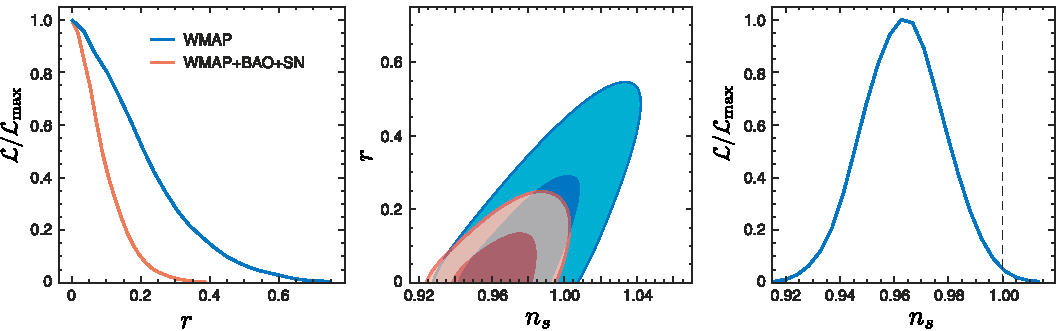
\includegraphics[width=.95\textwidth]{WMAP5_ns_r}
   \caption{インフレーションのパラメータ$n_s$と$r$に対する{\sl WMAP} 5年観測の制限\cite{WMAP5}．{\sl WMAP}だけの結果は青で，{\sl WMAP}に他の宇宙論的観測を加えた制限は赤で示す．
第3の図では，$r$は無視できると仮定している．
}%\newline [{\tt Placeholder.} {\tt Figure will be updated.}]}
    \label{fig:WMAP5}
\end{figure}



\subsubsection{ガウス性}

$\R$がガウス的なら，パワースペクトル$P_\R(k)$（実空間での2点相関）で話は完結する．
しかし，$\R$が{\it 非ガウス的}なら，揺らぎはゼロでないバイスペクトル$B_\R(k_1, k_2, k_3)$（実空間での3点相関に対応）をもつ．
ガウス的である仕方は一つしかないが，非ガウス的である仕方は多くあるので，非ガウス性への制限を述べるのは少し難しい．
非ガウス性の最も簡単な形の一つは，次のパラメータ化で記述される．
\beq
\label{equ:local2}
\R({\bf x}) = \R_g({\bf x}) + \frac{3}{5} f_{\rm NL} \star \R_g^2({\bf x})\, .
\eeq
ここで，$\R_g$はガウス的である．この非ガウス性の{\it 局所型模型}では，情報は一つの数$f_{\rm NL}$にまとめられる．
Smith，Senatore，Zaldarriaga\cite{Smith:2009jr}による$f_{\rm NL}$の最新の制限は，
\beq
\label{equ:smith}
- 4 \ < \ f_{\rm NL} \ < \ 80 \quad \text{（信頼水準} \ \ 95\% \ \text{）}\, .
\eeq
$f_{\rm NL}$が100程度の値であることは，式(\ref{equ:local2})の$\R_g \sim 10^{-5}$への0.1\%の補正に対応することに注意しよう．
したがって，制限(\ref{equ:smith})は，CMBが0.1\%の精度でガウス的であることを意味する！ これは，通常インフレーションの勝利として称賛される，宇宙の曲率への制限よりも厳しい．
CMBはきわめてガウス的だが，必ずそうでなければならなかったわけではない．
しかし，インフレーションが正しければ，観測されるガウス性はむしろ自然な帰結である．\footnote{非ガウス性は，インフラトン場の{\it 相互作用}の尺度である．しかし，スローロールの力学が成り立つには，インフラトンの自己相互作用が非常に弱くなければならず（ポテンシャルが非常に平坦），非ガウス性は必然的に小さく，$f_{\rm NL} \sim {\cal O}(0.01)$となる\cite{malda}．}

\subsubsection{断熱性}

単一場インフレーションでは，大きなスケール（空間勾配を無視できるスケール）でのインフラトン場の揺らぎは，一様な背景場の軌道に沿った局所的な前進または後退と同一視できる．インフラトンの軌道に沿ったこのずれは，インフレーション後の宇宙の各領域の全密度に影響するが，異なる成分の相対密度の変動を生むことはできない．
したがって，単一場インフレーションは，全体の曲率摂動$\R$で特徴付けられる，純粋に{\it 断熱的}な原始密度摂動を生成する．
これは，宇宙流体（光子，ニュートリノ，バリオン，冷たい暗黒物質（CDM）粒子）のすべての摂動が，同じ曲率摂動$\R$から生じ，断熱性の性質$\delta(n_m/n_r) =0$，または次式を満たすことを意味する．
\beq
\label{equ:ad}
\frac{\delta \rho_m}{\rho_m} = \frac{3}{4} \frac{\delta \rho_r}{\rho_r}\, ,
\eeq
ここで，添字$m$は非相対論的な成分（バリオンまたはCDM）をまとめて表し，$r$は相対論的な成分（光子またはニュートリノ）を表す．
最新のデータには，条件(\ref{equ:ad})の破れは見られない\cite{WMAP5}．
そのような破れが見つかれば，多場インフレーションの明確な徴候となる（\S\ref{sec:iso}参照）．

\subsectionlink{スローロール模型の検証}

図\ref{fig:nsr}に，最も単純な単一場スローロール・インフレーション模型のいくつかに対する，現在の観測的制限を示す（{\bf 第1講}参照）．
将来の測定は，許される模型のパラメータ空間を大幅に狭めるだろう．

\begin{figure}[h!]
    \centering
        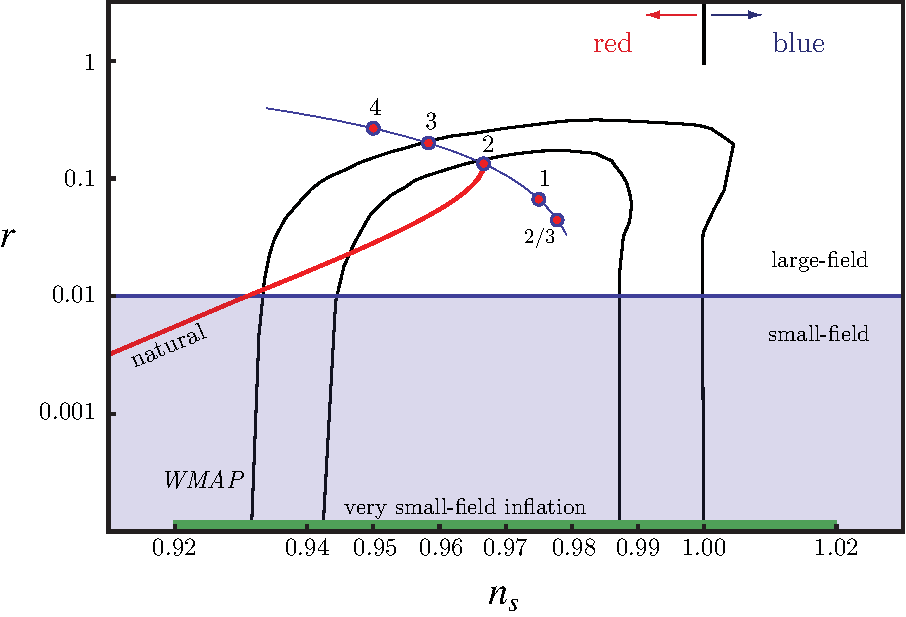
\includegraphics[width=.65\textwidth]{nsr}
   \caption{$n_s$-$r$平面上の単一場スローロール模型への制限．$r$の値は，模型における場の変位が大きいか小さいかを決める．$n_s$の値は，スカラー・スペクトルを赤いものと青いものに分類する．$r$と$n_s$の値の組合せにより，観測可能な宇宙が地平線を退出したとき，ポテンシャルの曲率が正（$\eta_{\rm v} > 0$）だったか負（$\eta_{\rm v} < 0$）だったかが決まる．
また，$n_s$と$r$に対する{\sl WMAP} 5年観測の制限\cite{WMAP5}と，単一場スローロール・インフレーションの代表的ないくつかの模型の予言も示す．
%\newline
{\it カオス的インフレーション}：$\lambda_p\, \phi^p$．一般の$p$（細い実線）と$p=4, 3, 2, 1, \frac{2}{3}$（{\large $\bullet$}）を示す．$p=2$~\cite{Nflation}，$p=1$~\cite{MSW}，$p=\frac{2}{3}$~\cite{Silverstein:2008sg}の模型は，最近，弦理論から得られた．
%\newline
{\it 自然インフレーション}：$V_0 [1-\cos(\phi/\mu)]$（実線）．
%{\it hill-top inflation}: $V_0 [1-(\phi/\mu)^2] + \dots$ (solid line);
%\newline
{\it 非常に小さな場のインフレーション}：非常に小さなテンソル振幅$r \ll 10^{-4}$をもつインフレーション模型（緑の帯）．弦理論における例として，ワープしたDブレーン・インフレーション\cite{KKLMMT, Baumann:2007ah, Baumann:2008kq}，ケーラー・インフレーション\cite{Conlon:2005jm}，レーストラック・インフレーション\cite{BlancoPillado:2006he}がある．}
    \label{fig:nsr}
\end{figure}


\sectionlink{インフレーションの将来の検証}

インフレーションの枠組みを本格的に検証する作業は，まだ始まったばかりである．
宇宙の平坦性と，密度揺らぎのほぼスケール不変な性質，ガウス性，断熱性は，インフレーションを支持する心強い証拠である\footnote{どの段階でも，インフレーションという考え方全体を反証する測定が得られた可能性があることに注意しよう．}が，インフレーションが実際に起こったことの証明ではない．\footnote{カール・ポパーは理論を決して証明できないと教えたのに，「証明」という言葉を使ってしまったことは承知している．}
そこで未来に目を向け，将来の実験がインフレーションの物理をどのようにさらに検証できるかを説明しよう．


\subsectionlink{テンソルモードの振幅}

おそらく，インフレーションの証拠として単独で最も重要なのは，原始テンソル振幅の測定であろう．
上で示したように，原始CMBの$B$モードが検出されれば，それをインフレーションの重力波以外で説明することは事実上不可能である\cite{BauZal}．
\beq
\fbox{$\displaystyle
C_\ell^{BB} \quad \Rightarrow \quad P_h(k) $}\, ,
\eeq
ここで，
\beq
\Delta^2_{\rm t}(k) \equiv \frac{k^3}{2\pi^2} P_h(k) = A_{\rm t} \left(\frac{k}{k_\star} \right)^{n_{\rm t}} \, .
\eeq
また，{\bf 第2講}では，テンソル振幅$A_t$がインフレーションのエネルギースケールに直接結び付くことを説明した．
インフレーションの物理に関する単独の手掛かりとして，これ以上に重要で，インフレーションの理論家が強く望むものがあるだろうか．
さらに，テンソルモードの検出は，インフラトン場が場の空間でプランクスケールを超える距離を動いたことを意味し，弦理論家や量子重力の愛好家に，インフラトン・ポテンシャルへのプランクスケールで抑制された補正を真剣に考えさせるだろう（{\bf 第5講}参照）．

\subsectionlink{スカラーモードのスケール依存性}

スペクトル指数$n_{\rm s}$のスケールによる変化（スペクトル指数の「ランニング」とも呼ばれる）は，スローロールの2次で初めて生じるので，小さいと期待される．
\beq
\alpha_{\rm s} \equiv \frac{d n_{\rm s}}{d \ln k} \sim {\cal O}(\varepsilon^2)\, .
\eeq
一方，予想に反する大きな正または負のランニングが見つかれば，インフレーションと摂動生成に関する最も単純な考え方の一部を見直す必要がある．

\subsectionlink{テンソルモードのスケール依存性}

インフレーションに由来する原始テンソル揺らぎの振幅を測定することは，観測上の大きな挑戦となる．
テンソル振幅が現在の上限に近くない限り，そのスケール依存性まで測定することを期待するのは現実的でないように思われる．
単一場スローロール模型では，テンソル・スカラー比$r$とテンソル・スペクトル指数$n_{\rm t}$は，{\it 整合性関係}によって結び付けられる．
\beq
\label{equ:cons}
r = - 8 n_{\rm t}\, .
\eeq
式(\ref{equ:cons})を測定することは，単一場スローロール・インフレーションを反証するための別の方法となる．

\subsectionlink{非ガウス性}

原始揺らぎは，非常に高い精度でガウス的である．
しかし，これから説明するように，わずかな非ガウス性にも，インフレーションの作用について膨大な情報が含まれる．
インフレーションの揺らぎの3点関数が，非ガウス統計を診断する主要な手段であることはすでに述べた．
運動量空間では，3点相関関数は一般に次のように書ける．
\beq
\langle \R_{{\bf k}_1} \R_{{\bf k}_2} \R_{{\bf k}_3} \rangle = (2\pi)^3\, \delta({\bf k}_1 + {\bf k}_2 + {\bf k}_3) \ f_{\rm NL} \ F(k_1, k_2, k_3)\, .
\eeq
ここで，$f_{\rm NL}$は非ガウス性の振幅を定義する無次元パラメータであり，関数$F(k_1, k_2, k_3)$が運動量依存性を担う．$f_{\rm NL}$の振幅と符号，および$F(k_1,k_2,k_3)$の形とスケール依存性は，非ガウス性を生成する相互作用の詳細に依存する．このため，3点関数は初期宇宙の模型を調べ，区別するための強力な道具となる\cite{NGreview}．

二つの非常に異なる機構によって，二つの単純で異なる形$F(k_1, k_2, k_3)$が生成される\cite{Babich_etal_04}．{\em 局所型の形}は多場模型に特徴的であり，その名は原始曲率摂動$\R$の実空間での表式に由来する．
\begin{equation}
\label{local} \R({\bf x}) = \R_g({\bf x}) + \frac{3}{5} f_{\rm NL}^{\rm local} \R_g({\bf x})^2\, ,
\end{equation}
ここで，$\R_g({\bf x})$はガウス確率場である．この表式をフーリエ変換すると，信号は$k_3 \ll k_1,k_2$という「押しつぶされた」三角形に集中することがわかる．局所型非ガウス性は，等曲率場（後述）の揺らぎが曲率摂動へ変換される多場模型で生じる．この変換は地平線の外側で起こり，そこでは勾配が重要でないため，式(\ref{local})の形の非線形性が生成される．この種類の具体的な模型には，多場インフレーション\cite{BMRmulti, Bernardeau:2002jy, Bernardeau:2002jf, Sasaki:2008uc, Naruko:2008sq, Byrnes:2008wi, Byrnes:2006fr, Langlois:2008vk, Valiviita:2008zb, Assadullahi:2007uw, Valiviita:2006mz, Vernizzi:2006ve, Allen:2005ye}，カーバトン・シナリオ\cite{Linde:1996gt, Lyth_etal03}，非一様再加熱\cite{Dvali:2003em, Kofman:2003nx}，新エクピロティック模型\cite{Creminelli:2007aq,Koyama_etal07,Buchbinder_etal07, Lehners:2007wc,Lehners:2008my, Koyama:2007ag, Koyama:2007mg}がある．
%In these cases, $|f_{\rm NL}^{\rm local}|$ is model-dependent but generically larger than $5-10$.

第2の重要な形は，$k_1 \sim k_2 \sim k_3$の配置で最大になるため，{\em 正三角形型}と呼ばれる．正三角形型は，DBIインフレーション\cite{Alishahiha:2004eh}，ゴースト・インフレーション\cite{GhostInflation,Senatore:2004rj}，およびより一般的な音速の小さい模型\cite{Creminelli:2003iq, Chen:2006nt}など，非正準運動項をもつ単一場模型によって生成される．

\subsectionlink{等曲率揺らぎ}
\label{sec:iso}

複数の場をもつインフレーション模型では，摂動は必ずしも断熱的ではない．
場が複数あると，全密度，したがって空間曲率に摂動がなくても，背景の軌道に直交する揺らぎが，異なる物質成分の相対密度に影響を与えうる\cite{Gordon:2000hv}．
このような{\it 等曲率}摂動（非断熱摂動またはエントロピー摂動とも呼ばれる）には，さまざまな可能性がある．例えば，CDMと光子の間の相対的な摂動を定義できる．
\beq
{\cal S}_m \equiv \frac{\delta \rho_m}{\rho_m} - \frac{3}{4} \frac{\delta \rho_\gamma}{\rho_\gamma}\, .
\eeq
断熱摂動と等曲率摂動は，CMB揺らぎに異なるピーク構造を生む．
したがって，CMB測定によって揺らぎの種類を区別でき，実際，等曲率摂動が（存在するとしても）劣勢の成分でなければならないことが，すでに示されている．

等曲率摂動は断熱摂動と相関している可能性がある．これを表すため，次の相関パラメータを定義する．
\beq
\beta \equiv \frac{P_{{\cal S} {\cal R}}}{\sqrt{P_{\cal S} P_\R}}\, ,
\eeq
ここで，$P_{\cal R}$と$P_{\cal S}$は，それぞれ断熱揺らぎと等曲率揺らぎのパワースペクトルであり，$P_{{\cal S} \R}$はその相互相関である．
2種類の摂動の相対振幅を係数$\alpha$でパラメータ化する．
\beq
\frac{P_{\cal S}}{P_\R} \equiv \frac{\alpha}{1-\alpha}\, ,
\eeq
等曲率成分の寄与への現在の制限は，無相関の場合（$\beta =0$）には$\alpha_0 < 0.067$（信頼水準96\%），完全に反相関の場合（$\beta = -1$）には$\alpha_{-1} < 0.0037$（信頼水準95\%）である．

等曲率摂動の振幅の理論予言は，模型に強く依存するため複雑になる．等曲率振幅は，多場インフレーションの力学だけでなく，インフレーション後の時間発展にも依存する．インフレーション後にすべての粒子種が熱平衡にあり，それらの局所密度が（化学ポテンシャルがゼロで）温度だけによって一意に決まるなら，原始摂動は断熱的となる\cite{Lyth:2002my,Weinberg04b}．したがって，原始等曲率モードが存在するためには，少なくとも一つの場が，存在量が熱平衡によって決まらない粒子種（例えば脱結合後のCDM），またはバリオン数やレプトン数のような保存量子数に従う粒子種へ崩壊しなければならないことに注意するのが重要である．

\newpage
\sectionlink{{\sl まとめ}：第3講}

\vskip 10pt
宇宙マイクロ波背景放射（CMB）と大規模構造（LSS）の観測は，構造の種となる原始揺らぎのスペクトルを制限するために用いられる．
これにより，CMBとLSSの実験は初期宇宙を探る手段となる．
インフレーション期についてのこの情報を取り出すには，揺らぎの後期の時間発展を考慮しなければならない．
これは，{\sf CMBFAST}や{\sf CAMB}などの数値計算コードで行う．

\vskip 6pt
現在の観測は，インフレーションの基本的な予言と見事に一致している．
宇宙は平坦であり，ほぼスケール不変でガウス的かつ断熱的な密度揺らぎのスペクトルをもつ．揺らぎは，再結合時に地平線より大きかったスケールで，ゼロでない相関を示す．さらに，CMBスペクトルのピーク構造は，揺らぎがコヒーレントな位相で生成されたことの証拠である．

\vskip 6pt
インフレーションの将来の検証は，主としてCMB偏光の測定から得られるだろう．
CMB偏光の$B$モードは，インフレーションの重力波に特有の徴候である．
$B$モードの振幅は，インフレーションのエネルギースケールを直接測る．
さらに，非ガウス性の測定は，インフラトン場の相互作用を制限することにより，インフレーションの物理について豊富な情報をもたらす可能性がある．

\vskip 6pt
最後に，次の測定結果は，単一場スローロール・インフレーションを反証する．
\begin{itemize}
\item 大きな非ガウス性，$f_{\rm NL} > 1$．
\item ゼロでない等曲率摂動，$\alpha \ne 0$．
\item スカラー・スペクトルの大きなランニング，$|\alpha_{\rm s}| > 0.001$．
\item テンソルの整合性関係の破れ，$r \ne - 8 n_{\rm t}$．
\end{itemize}



%\newpage
%\sectionlink{{\sl Problem Set}: Lecture 3}

%\vskip 10pt


\newpage
%\part{Lecture 4: Advanced Topic: Non-Gaussianity}

\part{第4講：原始非ガウス性}

\vspace{0.5cm}
 \hrule \vspace{0.3cm}
\begin{quote}
{\bf 要旨}

\noindent
本講では，原始非ガウス性の研究における主要な理論的結果をまとめる．
ほとんどの結果は証明せずに述べるが，インフレーションの根源的な物理的起源を制約するうえでの意義を説明する．
非ガウス統計の基本的な診断量としてバイスペクトルを導入したのち，その運動量依存性がインフレーションの作用を探る強力な手段であることを示す．
大きな非ガウス性が生じるのは，インフレーション中にインフラトンの相互作用が重要な場合に限られる．このため，単一場のスローロール・インフレーションでは非ガウス性は観測不可能なほど小さいと予測される一方，複数の場，高階微分相互作用，または非標準的な初期状態をもつ模型では大きくなりうる．
最後に，原始非ガウス性の検出または制約に向けた観測の展望を論じて本講を終える．

\end{quote}
\vspace{0.1cm}  \hrule
 \vspace{0.5cm}


\sectionlink{準備}

{\it 非ガウス性}，すなわち宇宙論的揺らぎの相関への非ガウス的寄与の研究は，初期宇宙を探る重要な手段となりつつある~\cite{Komatsu:2009kd}．原始非ガウス性はインフラトンの{\it 相互作用}を直接測る量なので，それに対する制約からインフレーションのダイナミクスについて多くを学べる．
また，インフレーションの枠組みに代わるシナリオにも強い制約を課す~\cite{Creminelli:2007aq,Koyama_etal07,Buchbinder_etal07, Lehners:2007wc,Lehners:2008my, Koyama:2007ag, Koyama:2007mg}．


{\bf 第2講}では，インフレーションの作用を共動曲率摂動 $\R$ の2次まで展開した．この自由場の作用を用いて，パワースペクトル $P_\R(k)$ を計算できた．{\bf 第3講}で述べたように，揺らぎ $\R$ がガウス分布に従うなら，パワースペクトル（または2点相関関数）がすべての情報を含んでいる．\footnote{ガウス揺らぎでは3点関数とすべての奇数次の高次相関関数が消え，すべての偶数次の高次相関関数は2点関数で表せる．言い換えれば，ガウス揺らぎではすべての{\it 連結}高次相関関数が消える．}
しかし非ガウス揺らぎでは，2点関数を超える高次相関関数にインフレーションに関する追加情報が含まれる．
主要な非ガウス効果を計算するには，主要な非自明な相互作用項を取り込むために作用を3次まで展開する必要がある．これらの計算は代数的にかなり難しいため，本講では主な結果とその物理的解釈の概説にとどめる．詳細と導出については，Bartolo らによる包括的な総説~\cite{NGreview}とそこで引用されている文献を参照されたい．


\subsectionlink{バイスペクトルと局所型非ガウス性}

\subsubsection{バイスペクトル}

2点関数のフーリエ変換はパワースペクトルである：
\beq
\langle \R_{{\bf k}_1}  \R_{{\bf k}_2}    \rangle =(2\pi)^3 \delta({\bf k}_1 + {\bf k}_2 ) P_\R(k_1)\, . 
\eeq
同様に，3点関数に対応するフーリエ空間の量が{\it バイスペクトル}である：
\beq
\label{equ:bi}
\fbox{$\displaystyle
\langle \R_{{\bf k}_1}  \R_{{\bf k}_2}   \R_{{\bf k}_3} \rangle =(2\pi)^3 \delta({\bf k}_1 + {\bf k}_2 + {\bf k}_3)  B_\R({\bf k}_1,{\bf k}_2, {\bf k}_3) $}\, .
\eeq
ここで，運動量保存を課すデルタ関数は，背景の並進不変性の帰結である．
関数 $B_\R$ は引数について対称であり，スケール不変な揺らぎに対しては次数 $-6$ の斉次関数となる：
\beq
B_\R( \lambda {\bf k}_1, \lambda {\bf k}_2, \lambda {\bf k}_3) = \lambda^{-6} B_\R({\bf k}_1,{\bf k}_2, {\bf k}_3) \, .
\eeq
回転不変性により独立変数の数はさらに二つだけに減少し，例えば二つの比 $k_2/k_1$ と $k_3/k_1$ を選べる．

具体的なインフレーション模型の3点関数を計算するには，相互作用が存在する場合の真空の時間発展を慎重に扱う必要がある（2点関数では，この効果は高次である）．
付録Cでは，宇宙論的相関関数を計算するための ``in-in'' 形式を説明する~\cite{Schwinger:1960qe, Calzetta:1986ey,Jordan:1986ug, malda, Weinberg:2005vy}．実際には3点関数の計算は代数的に非常に煩雑になりうるので，本講では最終結果の引用にとどめる．
これらの3点関数の計算法の詳細だけで，一つの総説に値する．
%Information about the mechanism that created the primordial perturbations may be extracted both from the {\it amplitude} $f_{\rm NL}$ and a model-dependent {\it shape function} $b_\R(k_1, k_2 k_3)$
%\beq
%B_\R(k_1,k_2,k_3) = f_{\rm NL} \times b_\R(k_1, k_2 k_3)\, .
%\eeq

\subsubsection{局所型非ガウス性}

非ガウス性を現象論的にパラメータ化する初期の方法の一つは，ガウス摂動 $\R_g$ への非線形補正を用いるものであった~\cite{komatsu01}：
\beq
\label{equ:local}
\fbox{$\displaystyle
\R({\bf x}) = \R_g({\bf x}) + \frac{3}{5}f_{\rm NL}^{\rm local}\, \left[\R_g({\bf x})^2 - \langle \R_g({\bf x})^2\rangle \right]$}\, .
\eeq
この定義は実空間で局所的なので，{\it 局所型非ガウス性}と呼ばれる．
非ガウス性に対する実験的制約（{\bf 第3講}参照）は，式~(\ref{equ:local}) で定義されるパラメータ $f_{\rm NL}^{\rm local}$ に対して与えられることが多い．\footnote{式~(\ref{equ:local}) の係数3/5は慣習的なものである．非ガウス性は最初，ニュートン・ポテンシャルを用いて $\Phi({\bf x}) = \Phi_g({\bf x}) + f_{\rm NL}^{\rm local} \, \left[\Phi_g({\bf x})^2 - \langle \Phi_g({\bf x})^2\rangle \right]$ と定義されたが，このポテンシャルは物質優勢期には係数3/5を介して $\R$ と関係するためである．}
式~(\ref{equ:local}) を用いると，局所型非ガウス性のバイスペクトルが導かれる：
\beq
B_\R(k_1, k_2, k_3) = \frac{6}{5} f_{\rm NL}^{\rm local} \times \left[ P_\R(k_1) P_\R(k_2) + P_\R(k_2) P_\R(k_3)+ P_\R(k_3) P_\R(k_1)\right]\, .
\label{equ:LocalBi}
\eeq

\begin{thm}[局所型バイスペクトル]
式~(\ref{equ:bi}) と (\ref{equ:local}) から式~(\ref{equ:LocalBi}) を導け．
  \end{thm}
 
スケール不変なスペクトル $P_\R(k) = A k^{-3}$ に対しては，これは
\beq
\label{equ:localscale}
B_\R(k_1, k_2, k_3) = \frac{6}{5} f_{\rm NL}^{\rm local} \times A^2 \left[ \frac{1}{(k_1 k_2)^3}+ \frac{1}{(k_2 k_3)^3}+  \frac{1}{(k_3 k_1)^3}\right]\, .
\eeq

一般性を失わずに，運動量を $k_3 \le k_2 \le k_1$ となるように並べよう．
すると局所型非ガウス性のバイスペクトルは，最小の $k$（すなわち $k_3$）が非常に小さく，$k_3 \ll k_1 \sim k_2$ となるとき最大になる．
このとき，残り二つの運動量はほぼ等しい．
この{\it スクイーズド}極限では，局所型非ガウス性のバイスペクトルは
\beq
\lim_{k_3 \ll k_1 \sim k_2} B_\R(k_1, k_2, k_3) = \frac{12}{5} f_{\rm NL}^{\rm local} \times P_\R(k_1) P_\R(k_3)\, .
\eeq
\subsectionlink{非ガウス性の形状}
式~(\ref{equ:bi}) のデルタ関数は，バイスペクトルの三つのフーリエモードが閉じた三角形を形成することを課している．
異なるインフレーション模型は，異なる三角形の配置で最大の信号を予測する．この{\it 非ガウス性の形状}~\cite{Babich_etal_04}は，原始摂動を生み出した機構を探る強力な手段になりうる．

形状関数を次のように定義すると便利である：
\beq
{\cal S}(k_1,k_2, k_3) \equiv N (k_1 k_2 k_3)^2 B_\R(k_1, k_2, k_3)\, ,
\eeq
ここで $N$ は適切な規格化因子である．
よく議論される二つの形状は，{\it 局所型}模型（式~(\ref{equ:localscale}) 参照）
\beq
{\cal S}^{\rm local}(k_1, k_2, k_3) \propto \frac{K_3}{K_{111}}\, ,
\eeq
と，{\it 正三角形型}模型
\beq
{\cal S}^{\rm equil}(k_1, k_2, k_3) \propto \frac{\tilde k_1 \tilde k_2 \tilde k_3}{K_{111}}\, .
\eeq
ここでは，Fergusson と Shellard~\cite{Fergusson:2008ra}によって初めて定義された記法を導入した：
\bea
K_p &=& \sum_i (k_i)^p \quad \text{ただし} \quad K = K_1 \\
K_{pq} &=& \frac{1}{\Delta_{pq}} \sum_{i \ne j} (k_i)^p (k_j)^q \\
K_{pqr} &=& \frac{1}{\Delta_{pqr}} \sum_{i \ne j \ne l} (k_i)^p (k_j)^q (k_l)^q \\
\tilde k_{ip} &=& K_p - 2 (k_i)^p \quad \text{ただし} \quad \tilde k_i = \tilde k_{i1}\, ,
\eea
ここで $\Delta_{pq} = 1 + \delta_{pq}$ および $\Delta_{pqr} = \Delta_{pq}(\Delta_{qr} + \delta_{pr})$ であり，添字について和は取らない．この記法により，文献で議論されるますます複雑なバイスペクトルの式を大幅に圧縮できる．

上で論じたように，スケール不変な揺らぎではバイスペクトルは二つの比 $k_2/k_1$ と $k_3/k_1$ だけの関数である．そこで，再スケールした運動量を定義する：
\beq
x_i \equiv \frac{k_i}{k_1}\, .
\eeq
運動量は $x_3 \le x_2 \le 1$ となるように並べてある．三角不等式から $x_2 + x_3 > 1$ が成り立つ．
以下では ${\cal S}(1, x_2 , x_3)$ を図示する（図~\ref{fig:localequil}，\ref{fig:local}，\ref{fig:equil}参照）．
規格化は ${\cal S}(1,1,1) \equiv 1$ とする．
同等な配置を二重に表示しないために，三角領域 $1-x_2 \le x_3 \le x_2$ の外側では ${\cal S}(1, x_2, x_3)$ をゼロとする．
図~\ref{fig:localequil}から，局所型の形状の信号は $x_3 \approx 0$，$x_2 \approx 1$ に集中し，正三角形型の形状は $x_2 \approx  x_3 \approx 1$ でピークをもつことがわかる．図~\ref{fig:shapes}は，異なる三角形の形状が $x_2$--$x_3$ 平面でどのように分布するかを示している．
%Figs.~\ref{fig:local} and \ref{fig:equil} give contour plots of the local and equilateral shape functions.

\begin{figure}[h!]
    \centering
        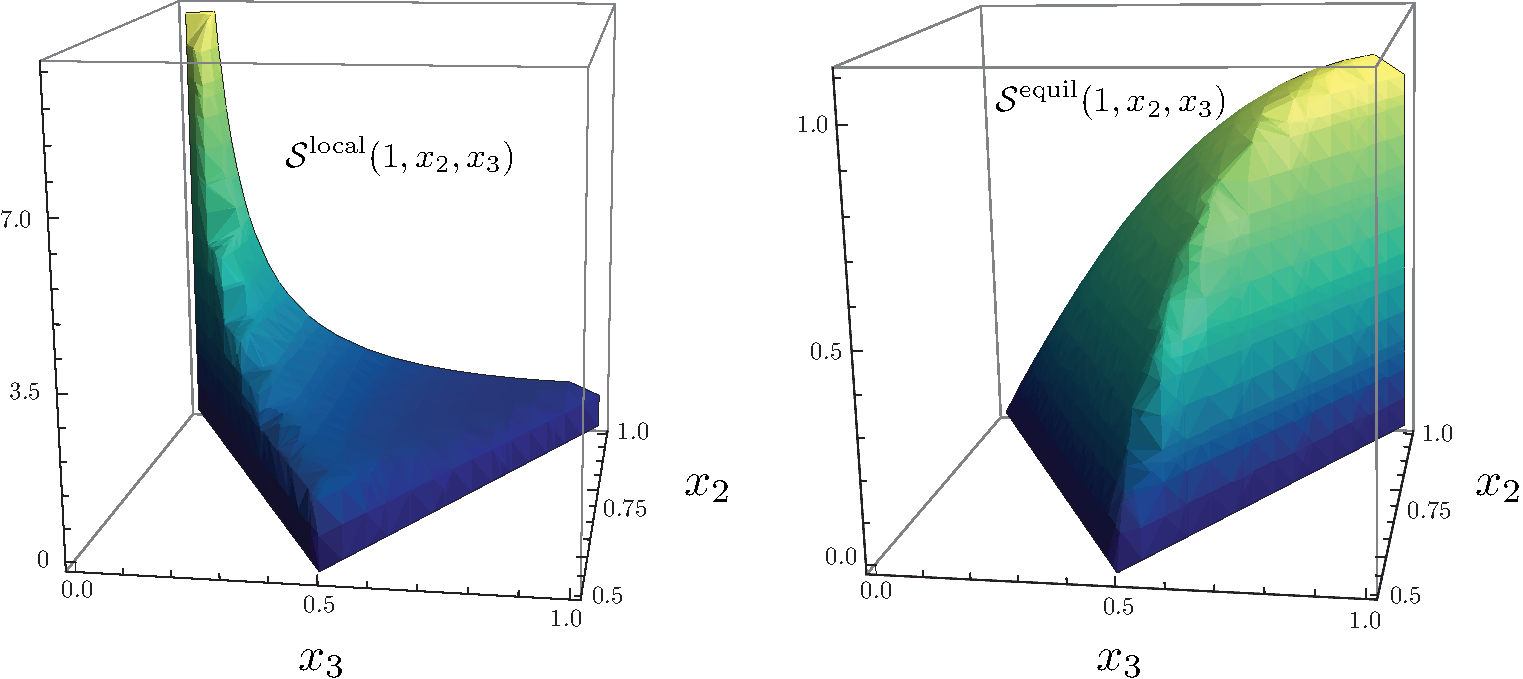
\includegraphics[width=.95\textwidth]{LocalEquil3D}
   \caption{{\it 局所型}および{\it 正三角形型}バイスペクトルの3次元表示．座標 $x_2$ と $x_3$ は，それぞれ再スケールした運動量 $k_2/k_1$ と $k_3/k_1$ である．運動量は $x_3 < x_2< 1$ となるように並べられ，三角不等式 $x_2 + x_3 > 1$ を満たす．}
    \label{fig:localequil}
\end{figure}

\begin{figure}[h!]
    \centering
        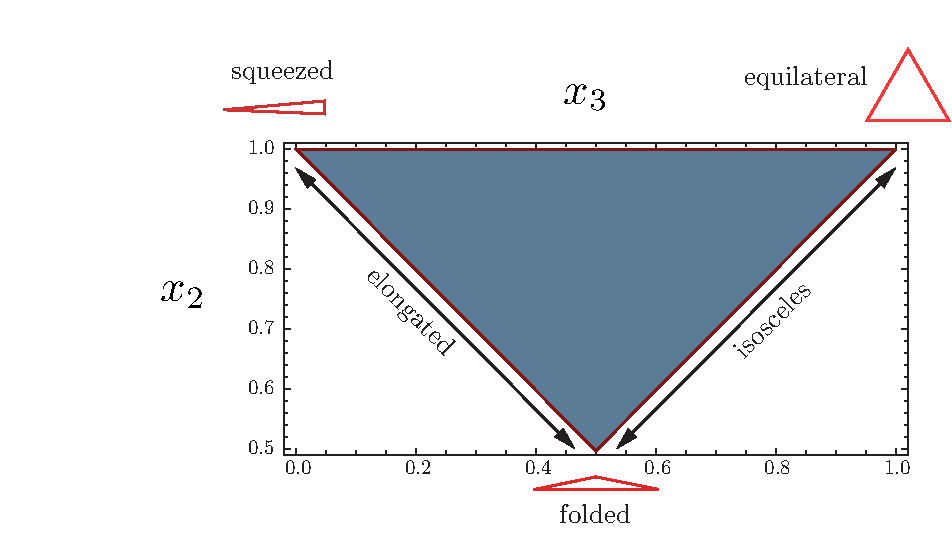
\includegraphics[width=.75\textwidth]{NGShapes}
   \caption{非ガウス性の形状．座標 $x_2$ と $x_3$ は，それぞれ再スケールした運動量 $k_2/k_1$ と $k_3/k_1$ である．運動量は $x_3 < x_2< 1$ となるように並べられ，三角不等式 $x_2 + x_3 > 1$ を満たす．}
    \label{fig:shapes}
\end{figure}

\begin{figure}[h!]
    \centering
        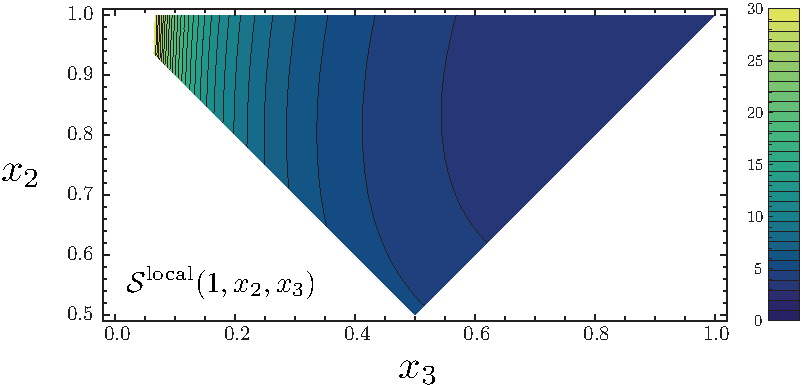
\includegraphics[width=.65\textwidth]{LocalContour}
   \caption{{\it 局所型}バイスペクトルの等高線図．}
    \label{fig:local}
\end{figure}

\begin{figure}[h!]
    \centering
        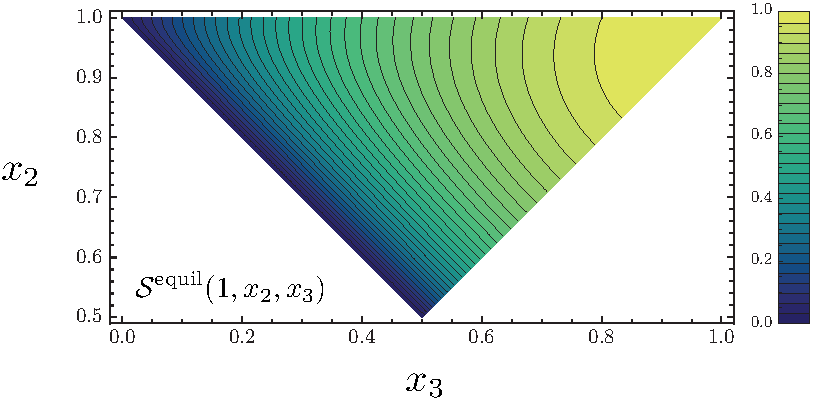
\includegraphics[width=.65\textwidth]{EquilContour}
   \caption{{\it 正三角形型}バイスペクトルの等高線図．}
    \label{fig:equil}
\end{figure}


非ガウス摂動を生成する物理的な動機をもつ模型は，特定の三角形配置でピークをもつ信号を生じることが多い．
重要な三つの特別な場合は次のとおりである：
\begin{enumerate}
\item[i)] {\it スクイーズド三角形}（$k_1 \approx k_2 \gg k_3$）

これは，インフレーション中に複数の軽い場をもつ模型~\cite{BMRmulti, Bernardeau:2002jy, Bernardeau:2002jf, Sasaki:2008uc, Naruko:2008sq, Byrnes:2008wi, Byrnes:2006fr, Langlois:2008vk, Valiviita:2008zb, Assadullahi:2007uw, Valiviita:2006mz, Vernizzi:2006ve, Allen:2005ye}，カーバトン・シナリオ~\cite{Linde:1996gt, Lyth_etal03}，不均一な再加熱~\cite{Dvali:2003em, Kofman:2003nx}，および新エクピロティック模型~\cite{Creminelli:2007aq,Koyama_etal07,Buchbinder_etal07, Lehners:2007wc,Lehners:2008my, Koyama:2007ag, Koyama:2007mg}において支配的なモードである．

\item[ii)] {\it 正三角形}（$k_1 = k_2 = k_3$）

正三角形でピークをもつ信号は，高階微分相互作用と非自明な音速をもつ模型で生じる~\cite{DBI, Chen:2006nt}．

\item[iii)] {\it 折り畳まれた三角形}（$k_1 = 2k_2 = 2 k_3$）

折り畳まれた三角形は，非標準的な初期状態をもつ模型で現れる~\cite{Holman:2007na, Chen:2006nt}．
\end{enumerate}

さらに，中間的な場合として，{\it 引き延ばされた三角形}（$k_1 = k_2 +k_3$）と{\it 二等辺三角形}（$k_1 > k_2 = k_3$）がある．



\subsectionlink{$f_{\rm NL}$：非ガウス性の振幅}

任意の形状関数に対して，一般化された $f_{\rm NL}$ パラメータを定義することで非ガウス性の大きさを測る：
\beq
\label{equ:gfNL}
\fbox{$\displaystyle f_{\rm NL} \equiv \frac{5}{18} \frac{B_\R(k,k,k)}{P_\R(k)^2} $}\, .
\eeq
この定義では，非ガウス性の振幅は正三角形配置で規格化される．

\begin{thm}[$f_{\rm NL}$]
式~(\ref{equ:LocalBi}) を用いて，定義~(\ref{equ:gfNL}) が式~(\ref{equ:local}) による $f_{\rm NL}^{\rm local}$ の定義と整合することを示せ．
  \end{thm}


\sectionlink{理論的予想}

\subsectionlink{単一場のスローロール・インフレーション}

スローロール・インフレーションが成立するには，インフラトン場の相互作用が弱くなければならない．自由場の基底状態の波動関数はガウス型であるため，スローロール・インフレーション中に生成される揺らぎもガウス型と予想される．
Maldacena~\cite{malda}は，スローロール（SR）インフレーションのバイスペクトルを初めて導出した：
\bea
{\cal S}^{\rm SR}(k_1, k_2, k_3) &\propto& ( \varepsilon - 2 \eta) \frac{K_3}{K_{111}} + \varepsilon \left(K_{12} + 8 \frac{K_{22}}{K} \right) \\
&\approx& (4 \varepsilon - 2 \eta) \, {\cal S}^{\rm local}(k_1, k_2, k_3) + \frac{5}{3} \varepsilon \, {\cal S}^{\rm equil}(k_1, k_2, k_3)\, , \label{equ:SSR}
\eea
ここで ${\cal S}^{\rm local}$ と ${\cal S}^{\rm equil}$ は，${\cal S}^{\rm local}(k,k,k) = {\cal S}^{\rm equil}(k,k,k)$ となるように規格化されている．
スローロール・インフレーションのバイスペクトルはスクイーズド三角形でピークをもち，その振幅はスローロール・パラメータによって抑制される~\cite{malda}：
\beq
f_{\rm NL}^{\rm SR} = {\cal O}(\varepsilon, \eta)\, . 
\eeq
スローロール・パラメータはインフラトンの自由場からのずれを特徴づけるので，これは直感にも合っている．

\subsectionlink{Maldacenaの定理}

単一場のインフレーションという仮定のもとで，インフレーションの作用については{\it ほかに何も}仮定せずに，Creminelli と Zaldarriaga~\cite{Creminelli:2004yq}は強力な定理を証明した： %first considered for the special case of slow-roll inflation by Maldacena:
\beq
\label{equ:CZ}
\fbox{$\displaystyle
\lim_{k_3 \to 0} \langle \R_{{\bf k}_1} \R_{{\bf k}_2} \R_{{\bf k}_3} \rangle = (2\pi)^3 \delta({\bf k}_1 + {\bf k}_2 + {\bf k}_3) \, \underline{\underline{(1-n_{\rm s})}} \, P_\R(k_1) P_\R(k_3) $} \, ,
\eeq
ここで
\beq
\langle \R_{{\bf k}_i} \R_{{\bf k}_j} \rangle = (2\pi)^3 \delta({\bf k}_i + {\bf k}_j) P_\R(k_i)\, .
\eeq
式~(\ref{equ:CZ}) は，単一場のインフレーションでは3点関数のスクイーズド極限が ($1-n_{\rm s}$) によって抑制され，完全にスケール不変な摂動では消えることを述べている．
したがって，スクイーズド極限で非ガウス性が検出されれば，単一場のインフレーションを排除できる！
特に，この主張はポテンシャルの形，運動項の形（または音速），および初期真空状態に依存しない．

\vspace{0.5cm}
 \hrule \vspace{0.3cm}
{\bf 証明}：

スクイーズド三角形は，一つの長波長モード $k_{\rm L} = k_3$ と二つの短波長モード $k_{\rm S}=k_1 \approx k_2$ を相関させる：
\beq
\langle \R_{{\bf k}_1} \R_{{\bf k}_2} \R_{{\bf k}_3} \rangle  \approx \langle (\R_{{\bf k}_{\rm S} })^2 \R_{{\bf k}_{\rm L}}\rangle\, .
\eeq
波長の長いモードほど早く凍結する．したがって，二つの短波長モードが凍結する時点で $k_{\rm L}$ はすでに地平線の外で凍結しており，それらに対する背景場として作用する．

なぜ $(\R_{{\bf k}_{\rm S} })^2$ は $\R_{{\bf k}_{\rm L}}$ と相関するのだろうか．
定理によれば，「$\R_{\rm k}$ が厳密にスケール不変なら相関しない」．
証明は実空間で最も簡単になる（Creminelli と Zaldarriaga~\cite{Creminelli:2004yq}参照）：
長波長の曲率摂動 $\R_{{\bf k}_{\rm L}}$ は，あるハッブル領域内の空間座標を再スケールする（あるいは有効なスケール因子を変える）：
\beq
\d s^2 =  - \d t^2 + a(t)^2 e^{2\R} \d {\bf x}^2\, .
\eeq
2点関数 $\langle \R_{{\bf k}_1} \R_{{\bf k}_2} \rangle$ は，地平線の外ですでに凍結している背景揺らぎ $\R_{{\bf k}_{\rm L}}$ の値に依存する．位置空間では，長波長揺らぎ $\R_{\rm L}$ による2点関数の変化は，線形の次数で
\beq
\label{equ:4}
\frac{\partial}{\partial \R_{\rm L}} \langle \R(x) \R(0) \rangle \cdot \R_{\rm L} = x \frac{d}{dx} \langle \R(x) \R(0) \rangle \cdot \R_{\rm L} \, .
\eeq 
3点関数を得るために，Creminelli と Zaldarriaga は式~(\ref{equ:4}) に $\R_{\rm L}$ を掛け，それについて平均を取る．
フーリエ空間に移ると式~(\ref{equ:CZ}) が得られる．\footnote{詳細は Cheung ら~\cite{Cheung:2007sv}を参照．}
証明終．
\vspace{0.2cm}  \hrule
 \vspace{0.5cm}
 

\subsectionlink{大きな非ガウス性をもつ模型}

\subsubsection{高階微分相互作用}


Maldacena は単一場の{\it スローロール}・インフレーションでは非ガウス性が常に小さいことを証明したが，インフレーション中に高階微分項が重要であれば，単一場の模型でも大きな非ガウス性を生じうる（スローロール・インフレーションで仮定する正準的な運動項と高階微分補正の不在を緩める）．
次の作用を考えよう：
\beq
S = \frac{1}{2} \int \d^4 x \sqrt{-g} \left[ R - P(X, \phi)\right]\, , \quad \text{ただし} \quad X \equiv (\partial_\mu \phi)^2\, .
\eeq
ここで $P(X, \phi)$ は運動項 $X=(\partial_\mu \phi)^2$ の任意の関数であり，したがって高階微分相互作用を含みうる．
これらの模型では一般に，揺らぎの伝播の音速が非自明になる：
\beq
c_s^2 \equiv \frac{P_{,X}}{P_{,X} + 2 X P_{,XX}}\, .
\eeq

$\R$ の2次の作用（$P_\R$ を与える）は~\cite{Chen:2006nt}
\beq
S_{(2)} = \int \d^4 x \, \varepsilon \left[ a^3 (\dot \R)^2/ \underline{\underline{c_s^2}} - a (\partial_i \R)^2\right] + {\cal O}(\varepsilon^2)
\eeq
$\R$ の3次の作用（$B_\R$ を与える．付録~\ref{sec:inin}および文献~\cite{Chen:2006nt}参照）は
\beq
\label{equ:s3}
S_{(3)} = \int \d^4 x\, \underline{\underline{\varepsilon^2}} \left[ \dots a^3 (\dot \R)^2 \R/ \underline{\underline{c_s^2}} + \dots a (\partial_i \R)^2 \R + \dots a^3 (\dot \R)^3/ \underline{\underline{c_s^2}} \right] + {\cal O}(\varepsilon^3)
\eeq
3次の作用が2次の作用に比べて余分な $\varepsilon$ の因子によって抑制されていることに注目しよう．
これは，スローロール極限 $P(X, \phi) = X- V(\phi)$，$c_s^2 = 1$ で非ガウス性が小さいことの現れである．
しかしスローロール極限から離れ，音速が小さく $c_s^2 \ll 1$ なる場合には，式~(\ref{equ:s3}) のいくつかの相互作用項が増幅され，非ガウス性が大きくなりうる．
信号は正三角形でピークをもち，
\beq
\label{equ:Lequil:source-duplicate-1}
f_{\rm NL}^{\rm equil} = - \frac{35}{108} \left( \frac{1}{c_s^2} -1 \right) + \frac{5}{81} \left( \frac{1}{c_s^2} - 1 - 2 \Lambda \right)\, ,
\eeq
ここで
\beq
\Lambda \equiv \frac{X^2 P_{,XX} + \frac{2}{3} X^3 P_{,XXX}}{X P_{,X} + 2 X^2 P_{,XX}}\, .
\eeq
任意の $P(X,\phi)$ をもつ作用が整合的な高エネルギー理論に存在するかどうかは，これらの模型にとって重要な課題である．
弦理論における最も興味深いインフレーション模型の一つであるDBIインフレーション~\cite{DBI}（{\bf 第5講}参照）が，まさにこのような構造をもつことは心強い：
\beq
P_{\rm DBI}(X, \phi) = - f^{-1}(\phi) \sqrt{1-2 f(\phi) X} + f^{-1}(\phi) - V(\phi)\, .
\eeq
この場合，式~(\ref{equ:Lequil}) の第2項は恒等的にゼロとなり，次を得る：
\beq
\label{equ:Lequil}
f_{\rm NL}^{\rm DBI} = - \frac{35}{108} \left( \frac{1}{c_s^2} -1 \right) \, .
\eeq
DBIインフレーションの形状関数は
\beq
\label{equ:SDBI}
{\cal S}^{\rm DBI}(k_1,k_2,k_3) \propto \frac{1}{K_{111} K^2} (K_5+ 2 K_{14} - 3 K_{23} +2 K_{113}-8 K_{122})\, .
\eeq

\subsubsection{複数の場}

単一場のスローロール・インフレーションでは，インフラトンの相互作用はインフレーションが生じるという要請によって制約される．
しかし，インフレーション中に複数の場が重要であれば，この制約を回避できる．{\it カーバトン機構}~\cite{Linde:1996gt, Lyth_etal03}や{\it 不均一な再加熱}~\cite{Dvali:2003em, Kofman:2003nx}のような模型は，この点を利用し，インフラトンとは別の第2の場の揺らぎを通して非ガウス揺らぎを生成する．
信号はスクイーズド三角形でピークをもつ．

局所型非ガウス性を生むこれらの機構の詳細については，Bartolo らの総説~\cite{NGreview}を参照されたい．

\subsubsection{非標準的な真空}

インフレーションがBunch--Davies真空ではなく励起状態から始まったなら，残存する非ガウス性が観測可能かもしれない~\cite{Holman:2007na}（ただしインフレーションが最小限の $e$-fold数を大幅に超えて継続した場合には，この効果は指数関数的に希釈される）．
信号は折り畳まれた三角形でピークをもち，その形状関数は
\beq
\label{equ:Sfolded}
{\cal S}^{\rm folded}(k_1,k_2,k_3) \propto \frac{1}{K_{111}} (K_{12} - K_3) + 4 \frac{K_2}{(\tilde k_1 \tilde k_2 \tilde k_3)^2}\, .
\eeq
この効果のより詳しい議論については，Holman と Tolley の論文~\cite{Holman:2007na}を参照されたい．

 
\sectionlink{観測の展望}


原始非ガウス性に対する観測的制約は，興味深い水準に達し始めている．
高精度CMB実験は現在，一部のインフレーション模型~\cite{Linde:1996gt, Lyth_etal03, Dvali:2003em, Kofman:2003nx}と，新エクピロティック模型の大半~\cite{Creminelli:2007aq,Koyama_etal07,Buchbinder_etal07, Lehners:2007wc,Lehners:2008my, Koyama:2007ag, Koyama:2007mg}が信号を予測するパラメータ空間の領域を調べている．

\subsectionlink{宇宙マイクロ波背景放射}

Smith，Senatore，Zaldarriaga~\cite{Smith:2009jr, Senatore:2009gt}による $f_{\rm NL}^{\rm local}$ および $f_{\rm NL}^{\rm equil}$ への最新の制約は
\begin{align}
- 4& \ < \ f_{\rm NL}^{\rm local} \ < \ \ +80 \quad \text{（信頼水準} \ \ 95\% \ \text{）}\, , \\
- 125& \ < \ f_{\rm NL}^{\rm equil} \ < \ \ +435 \quad \text{（信頼水準} \ \ 95\% \ \text{）}\, .
\end{align}
Planck衛星と提案中のCMBPolミッションでは，それぞれ $\sigma(f_{\rm NL}^{\rm local}) \sim 5$ と $\sigma(f_{\rm NL}^{\rm local}) \sim 2$ が得られると予測されている．
実際，$f_{\rm NL} \sim {\cal O}(1)$ の水準では，インフレーションとは無関係な二次効果からの信号が見えると予想される．これらの効果を原始信号と混同しないためには，揺らぎの非線形発展がそれ自身の非ガウス性をどのように誘起するかを詳細に計算する必要がある．
現時点で，これらの効果はまだ完全には計算されていない（ただし，例えば文献~\cite{BMR1, BMR2, Senatore:2008wk}参照）．
多くの場合，その大きさのオーダーだけが見積もられている．観測可能な水準の非ガウス性を誘起するすべての効果を系統的に特徴づけることは，明らかに時宜にかなっている．




\subsectionlink{大規模構造}

非ガウス性は宇宙の大規模構造にも痕跡を残す．
一般に，大規模構造の観測から原始非ガウス性を取り出すことは，非線形揺らぎが原始起源の信号を完全に圧倒する非ガウス性を生むために難しくなる．
しかし最近，原始非ガウス性を探る有望な手段として{\it スケール依存バイアス}の概念が導入された~\cite{Dalal:2007cu, Slosar:2008hx}．
基礎にある密度場を大きなバイアスでたどるトレーサーでは，バイアス・パラメータがスケールと $f_{\rm NL}$ に依存することが示されている~\cite{Dalal:2007cu, Slosar:2008hx}：
\beq
P_{\delta_g}(k) = \left[b+ \Delta b(k, f_{\rm NL}^{\rm local})\right]^2 P_\delta(k)\, .
\eeq
この手法の詳細は本講の範囲を超えるが，例えば文献~\cite{Slosar:2008hx}に述べられている．
この手法をSDSSの高光度赤色銀河（LRG）のサンプルに適用すると，次が得られる~\cite{Slosar:2008hx}：
\beq
- 29 \ < \ f_{\rm NL}^{\rm local} \ < \ + 70 \quad \text{（信頼水準} \ \ 95\% \ \text{）}\, .
\eeq
この上限がCMBから得られた制約に匹敵することに注意しよう．
原始非ガウス性の真に頑健な検証とするにはさらなる研究が必要だが，Slosar らによる予備的な結果~\cite{Slosar:2008hx}は，この手法の原理を実証する心強いものとなっている．

\newpage
\sectionlink{{\sl まとめ}：第4講}

\vskip 10pt


宇宙論的揺らぎの相関に対する非ガウス的寄与の研究は，初期宇宙を探る重要な手段となりつつある~\cite{Komatsu:2009kd}．非ガウス性はインフラトンの相互作用を直接測る量なので，インフレーションのダイナミクスについて多くを教えてくれる可能性がある．

非ガウス揺らぎの基本的な診断量は，3点関数またはバイスペクトルである：
\beq
\langle \R_{{\bf k}_1}  \R_{{\bf k}_2}   \R_{{\bf k}_3} \rangle =(2\pi)^3 \delta({\bf k}_1 + {\bf k}_2 + {\bf k}_3)  B_\R(k_1, k_2, k_3) \, .  \nonumber
\eeq

非ガウス摂動を生成する物理的な動機をもつ模型は，特定の三角形配置でピークをもつ信号を生むことが多い．
三つの特別な場合は次のとおりである：
\begin{enumerate}
\item[i)] {\it スクイーズド三角形}（$k_1 \approx k_2 \gg k_3$）

これは，インフレーション中に複数の軽い場をもつ模型~\cite{BMRmulti, Bernardeau:2002jy, Bernardeau:2002jf, Sasaki:2008uc, Naruko:2008sq, Byrnes:2008wi, Byrnes:2006fr, Langlois:2008vk, Valiviita:2008zb, Assadullahi:2007uw, Valiviita:2006mz, Vernizzi:2006ve, Allen:2005ye}，カーバトン・シナリオ~\cite{Linde:1996gt, Lyth_etal03}，不均一な再加熱~\cite{Dvali:2003em, Kofman:2003nx}，および新エクピロティック模型~\cite{Creminelli:2007aq,Koyama_etal07,Buchbinder_etal07, Lehners:2007wc,Lehners:2008my, Koyama:2007ag, Koyama:2007mg}において支配的なモードである．

\item[ii)] {\it 正三角形}（$k_1 = k_2 = k_3$）

正三角形でピークをもつ信号は，高階微分相互作用をもつ模型で生じる~\cite{DBI}．

\item[iii)] {\it 折り畳まれた三角形}（$k_1 = 2k_2 = 2 k_3$）

折り畳まれた三角形は，非標準的な初期状態をもつ模型で現れる~\cite{Holman:2007na}．
\end{enumerate}

\begin{figure}[h!]
    \centering
        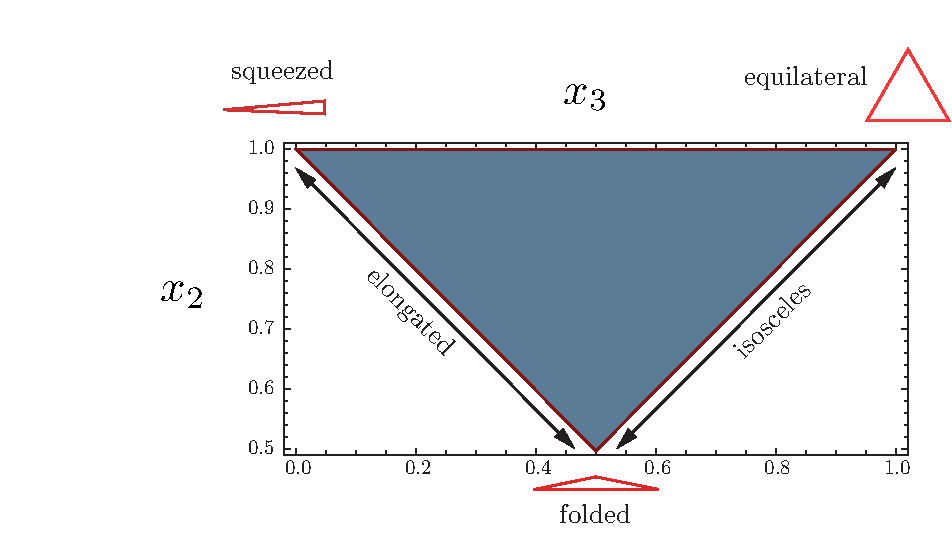
\includegraphics[width=.75\textwidth]{NGShapes}
   \caption{非ガウス性の形状．三角形の形状は，再スケールした運動量 $x_2 = k_2/k_1$，$x_3=k_3/k_1$ によってパラメータ化される．}
    \label{fig:shapes2}
\end{figure}
単一場の整合性関係は
\beq
\lim_{k_3 \to 0} \langle \R_{{\bf k}_1} \R_{{\bf k}_2} \R_{{\bf k}_3} \rangle = (2\pi)^3 \delta({\bf k}_1 + {\bf k}_2 + {\bf k}_3) \, \underline{\underline{(1-n_{\rm s})}} \, P_\R(k_1) P_\R(k_3)  \, . \nonumber
\eeq
これは，単一場のインフレーションのバイスペクトルのスクイーズド極限が，スケール不変性からのずれ $1- n_{\rm s}$ に比例することを述べている．


\sectionlink{{\sl 演習問題}：第4講}

\vskip 10pt
\begin{thmP}[バイスペクトルの図示]\label{ex:bispectra}

局所型および正三角形型のバイスペクトルの図（それぞれ図~\ref{fig:local}と図~\ref{fig:equil}）を再現せよ．
続いて，スローロール・インフレーション，DBI模型，および励起した初期状態をもつ模型のバイスペクトル，すなわち ${\cal S}^{\rm SR}(1,x_2,x_3)$（式~(\ref{equ:SSR})），${\cal S}^{\rm DBI}(1,x_2,x_3)$（式~(\ref{equ:SDBI})），${\cal S}^{\rm folded}(1,x_2,x_3)$（式~(\ref{equ:Sfolded})）を図示せよ．


\end{thmP}
\newpage


\newpage
%\part{Lecture 4: Advanced Topic: Non-Gaussianity}
\part{第5講：弦理論におけるインフレーション}

\vspace{0.5cm}
 \hrule \vspace{0.3cm}
\begin{quote}
{\bf 要旨}

\noindent
この連続講義の最後に，少し高度な話題である弦理論におけるインフレーションを論じる．
Liam McAllisterとの最近の総説論文~\cite{BMReview}に基づき，この主題を教育的に概説する．
本講の中心的な主題は，インフレーションのプランク・スケールの物理に対する感度である．これこそが弦理論でインフレーションを実現する主要な動機であると同時に，中心的な理論的課題でもあると論じる．
弦理論におけるインフレーション・シナリオの二つの事例，ワープしたDブレーン・インフレーションとアクシオン・モノドロミー・インフレーションを通じて，これらの問題を具体的に示す．
最後に，理論面と観測面の両方における今後の進展の可能性を示す．
\end{quote}
\vspace{0.1cm}  \hrule
 \vspace{0.5cm}


\sectionlink{なぜ二つの思弁的な考えを結びつけるのか？}

これまでの講義で，インフレーションが極初期宇宙のダイナミクスの現象論的模型として際立って成功していることを見てきた．しかし，インフレーション的膨張の物理的起源の詳細な理解は，依然として得られていない．
インフレーションと弦理論はいずれも，最高エネルギーでの物理的宇宙を理解しようとする野心的な試みである．
どちらも思弁的な理論であり，実験による確認を待っている．
したがって，なぜ今，弦理論におけるインフレーションという問題に取り組むべきなのかと疑問に思うかもしれない．

本講では，場の量子論と重力の紫外（UV）完備化，すなわちプランク・スケールに近づくエネルギーでの場の内容と相互作用に敏感に依存する，インフレーションの特定の側面を取り上げる．このような問題を最も自然に扱えるのはプランク・スケールの物理の理論であり，弦理論はおそらくその最も発展した候補である．これが，弦理論でインフレーションの物理を理解しようとする動機である．

\S\ref{sec:ST}の弦理論による構成の詳細にはあまり関心がない読者にも，\S\ref{sec:UV}の有効場理論に基づく一般的な議論は参考になるだろう．
 
\sectionlink{インフレーションの紫外物理に対する感度}
\label{sec:UV}


\subsectionlink{有効場理論とインフレーション}
\label{sec:eft}

\begin{figure}[h!]
	\centering
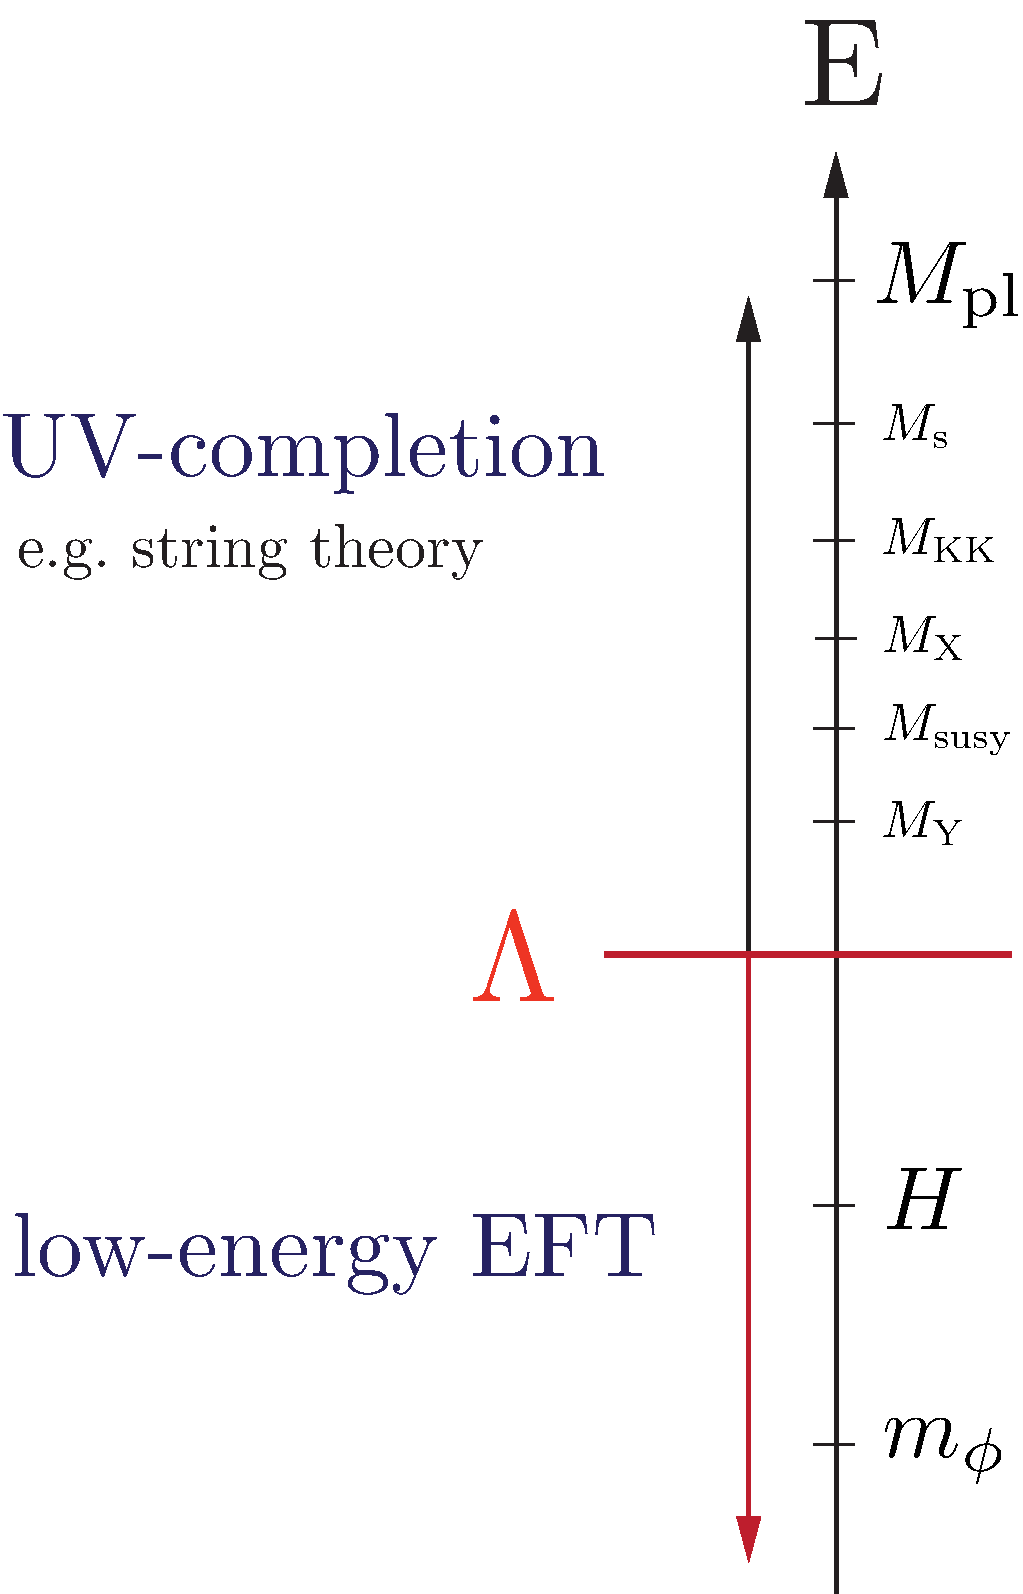
\includegraphics[width=.31\textwidth]{EFT}
%\vspace{-0.5cm}
\caption{インフレーションの有効場理論（EFT）．EFTのカットオフ $\Lambda$ は，低エネルギー理論のスペクトルに含まれない最も軽い粒子の質量によって定義される．カットオフを超える質量をもつ粒子は積分消去され，インフラトンなどの軽い場のラグランジアンに補正を与える．}
\label{fig:EFT}
\end{figure}

一般相対論に結合した場の量子論の現象として見ると，インフレーションは自然とは思われない．特に，インフレーションに適したラグランジアンの集合は，可能なすべてのラグランジアンの集合のごく小さな部分集合である．
さらに，広い範囲の模型で，インフレーションはかなり特殊な初期条件のもとでしか生じない．例えば小場シナリオでは，初期の運動エネルギーがごく小さい配置が必要となる．インフレーションを生むラグランジアンと初期条件の双方の自然さを調べて定量化したいところだが，初期条件の問題は，永遠のインフレーションにおける測度を理解しようとする，活発ではあるものの未完成な研究計画と切り離せないように見える（批判的な評価は\S\ref{sec:conclusion}参照）．
 % \cite{eternal}.
% (However, see {\it e.g.}~\cite{initial} for recent efforts to quantify or to ameliorate the fine-tuning of initial conditions.) 
本講では，インフレーションに適したラグランジアンをもつことがどれほど自然（または不自然）であるかという問題に集中する．

正準的な運動項をもつ単一のインフラトン場では，インフレーションの必要条件をインフラトン・ポテンシャルで表せる（{\bf 第1講}参照）．
インフレーションには，プランク単位で非常に平坦なポテンシャルが必要である：
 \beq
 \epsilon_{\rm v} = \Mp^2 \left(\frac{V_{,\phi}}{V}  \right)^2 \ll 1\, , \qquad \eta_{\rm v} = \frac{\Mp^2}{2} \frac{V_{, \phi \phi}}{V} \ll 1\, .
 \eeq
これから論じるように，この条件はプランク・スケールの物理に敏感である．

$W$--$W$ 散乱のユニタリティが ${\rm TeV}$ スケールの新しい物理を要求するのと同様に，重力子同士の散乱を整合的にするためには，プランク・スケールで何らかの新しい物理が必要であることを思い出そう．新しい自由度が現れなければならないことはわかっているが，プランク・スケールの物理が弦理論のような有限な量子重力理論なのか，それともさらに高いスケールの未知の物理に対する単なる有効理論なのかはわからない．しかし，プランク・スケールの理論の構造は，インフラトン・ポテンシャルの形に有意義な，そして非常に好都合な場合には検証可能な帰結をもたらす．

通常どおり，あるカットオフ $\Lambda$ を超える高スケールの物理の効果は，低エネルギー有効理論の演算子の係数によって効率よく記述される（図~\ref{fig:EFT}参照）．質量 $M \ge \Lambda$ の粒子を積分消去すると，次の形の演算子が生じる：
\begin{equation}
\label{equ:ODelta}
\fbox{$\displaystyle \frac{{\cal{O}}_{\delta}}{M^{\delta-4}} $}\, ,
\end{equation}
ここで $\delta$ は演算子の質量次元を表す．

このような演算子に対する感度は，素粒子物理ではありふれている．例えば，フレーバーを変える過程に対する制限は ${\rm TeV}$ スケールを超える物理を制限し，陽子の寿命の下限からは，陽子崩壊を媒介するGUTスケールの演算子さえ制約できる．
しかし，素粒子物理の考察だけでは，次元 $\delta=6$ を超える演算子や $M\sim M_{\rm GUT}$ を超えるスケールにまで届くことは少ない．（重力を媒介とする超対称性の破れのシナリオは例外の一つである．）同じことを言い換えると，プランク・スケールの過程や非常に高い次元の演算子は，素粒子物理の大部分には無関係であり，低エネルギー現象から分離している．

しかしインフレーションでは，プランク単位でのポテンシャルの平坦性によって，次のような $\delta\le 6$ の{\it プランク・スケールで抑制された}演算子に対する感度が生じる：
\begin{equation}
\label{equ:O6}
\frac{{\cal{O}}_{6}}{M_{\rm pl}^{2}}\, .
\end{equation}
etaパラメータの小ささを論じるには，すなわち理論が少なくとも60~$e$-foldのインフレーション的膨張を可能にすることを保証するには，このような演算子を理解する必要がある．したがって，次元6のプランク・スケールで抑制された演算子に対するこの感度は，すべてのインフレーション模型に共通する．

大場インフレーション模型では，インフラトン作用の紫外物理に対する感度が劇的に高まる．
この重要な種類のインフレーション模型では，ポテンシャルは任意の次元の演算子からなる{\it 無限}級数に敏感になる（\S\ref{sec:lyth}参照）．


\subsectionlink{eta問題}

インフラトン・ポテンシャルを保護する特定の対称性がない場合，ラグランジアンへの寄与として次の一般的な形が
\beq
\fbox{$\displaystyle
\frac{{\cal O}_6}{M_{\rm pl}^2}\, = \, \frac{{\cal O}_4}{M_{\rm pl}^2}\, \phi^2$}\,
\eeq
許される．
次元4の演算子 ${\cal O}_4$ の真空期待値（vev）がインフレーションのエネルギー密度に匹敵し，$\langle{\cal O}_4 \rangle \sim V$ なら，この項はインフラトンの質量に $H$ 程度の補正を，同じことだがetaパラメータに1程度の補正を与え，インフレーション模型の構築に重大な問題をもたらす．
この形の寄与は，プランク・スケールの自由度を積分消去することで生じると考えられる点を，改めて強調しておく．
本節では，このいわゆる{\it eta問題}をまず\S\ref{sec:higgs}で有効場理論において論じ，次に\S\ref{sec:sugraETA}で超重力の例を用いて具体的に示す．

\subsubsection{インフラトン質量の放射不安定性}
\label{sec:higgs}

カットオフ $\Lambda$ をもつ一般的な有効理論（図~\ref{fig:EFT}参照）では，スカラー場の質量は何らかの対称性に保護されていない限りカットオフ・スケールまで走る．
インフレーションの有効理論のカットオフは少なくともハッブル・スケール以上，$\Lambda \ge H$ なので，これは小さなインフラトン質量（$m_\phi \ll H$）が放射補正に対して不安定であることを意味する．
同じことを言えば，etaパラメータは放射補正
\beq
\Delta\eta_{\rm v} = \frac{\Delta m_\phi^2}{3 H^2} \ge 1\, ,
\eeq
を受け，長く続くインフレーションを妨げる．

ここでの困難はヒッグスの階層性問題に似ているが，超対称性だけではインフラトン質量を安定化できない．インフレーションのエネルギーは必然的に超対称性を破り，その結果生じる超多重項内の分裂は $H$ 程度なので，超対称性は小さなインフラトン質量 $m_\phi \ll H$ を保護しない．

\S\ref{sec:LargeField}では，シフト対称性 $\phi\to\phi \, +\, const.$ によってインフラトン・ポテンシャルを保護するという自然な提案を論じる．これはインフラトンを擬南部--ゴールドストーン粒子と同定することに相当する．
このような対称性がなければ，eta問題は，インフレーションを得るためにその作用を微調整する必要があることを示しているように思われる．



\subsubsection{超重力の例}
\label{sec:sugraETA}

eta問題の重要な例は，局所的に超対称な理論，すなわち超重力において生じる~\cite{Copeland:1994vg}．
4次元超重力は超対称な弦コンパクト化の低エネルギー有効理論なので~\cite{PolchinskiOne, Polchinski}，この場合は多くの弦理論インフレーション模型に関係する．

${\cal N} = 1$ 超重力では，スカラー・ポテンシャルの重要な項がF項ポテンシャルである：
\beq
\label{equ:Fterm}
 V_F = e^{K/M_{\rm pl}^2} \left[ K^{\varphi \bar \varphi} D_{\varphi} W \overline{D_{\varphi} W} - \frac{3}{M_{\rm pl}^2} |W|^2 \right]\, ,
\eeq
ここで $K(\varphi, \bar \varphi)$ と $W(\varphi)$ はそれぞれケーラー・ポテンシャルと超ポテンシャルであり，$\varphi$ はインフラトンとする複素スカラー場である．また，$D_{\varphi}W \equiv \partial_{\varphi} W + M_{\rm pl}^{-2}(\partial_{\varphi} K) W$ と定義した．説明を簡単にするため，ほかに軽い自由度がないと仮定したが，ほかの場を含むように式を一般化することは容易である．

ケーラー・ポテンシャルはインフラトンの運動項 $-K_{,\varphi \bar \varphi} \, \partial \varphi \partial \bar \varphi$ を決め，超ポテンシャルは相互作用を決める．
インフラトン質量を導くため，ある原点のまわりで $K$ を展開する．一般性を失わずにこの原点を $\varphi \equiv 0$ と表すと，$K(\varphi, \bar \varphi) = K_0 + \left. K_{,\varphi \bar \varphi}\right|_0 \, \varphi \bar \varphi + \cdots\ $ である．するとインフレーションのラグランジアンは
\begin{eqnarray}
{\cal L} &\approx& - K_{,\varphi \bar \varphi}\, \partial \varphi  \partial \bar \varphi -  V_0 \Bigl(1+ \left. K_{,\varphi \bar \varphi}\right|_0 \frac{\varphi \bar \varphi}{M_{\rm pl}^2} + \dots \Bigr) \\
&\equiv& -  \partial \phi \partial \bar\phi - V_0 \Bigl(1+  \frac{\phi \bar \phi}{M_{\rm pl}^2} \Bigr) + \dots\, , \label{equ:mid}
\end{eqnarray}
ここで，正準的なインフラトン場 $\phi\bar\phi \approx  \left. K_{\varphi \bar \varphi}\right|_0 \varphi \bar \varphi$ と $V_0 \equiv \left. V_F\right|_{\varphi =0}$ を定義した．
式~(\ref{equ:Fterm}) の $e^{K/M_{\rm pl}^2}$ の展開に由来するポテンシャルへの主要な補正を残してある．これはF項シナリオにおける普遍的な補正と呼んでよいだろう．省略した項の一部は残した項と同じ程度になりうるが，それらは式~(\ref{equ:Fterm}) の
\beq\left[ K^{\varphi \bar \varphi} D_{\varphi} W \overline{D_{\varphi} W} - \frac{3}{M_{\rm pl}^2} |W|^2 \right]
\label{equ:md}
\eeq を展開することで生じ，ケーラー・ポテンシャルと超ポテンシャルの模型依存の構造に明らかに依存する．

結果は式~(\ref{equ:O6}) の形をもち，
\beq
{\cal O}_6 =   V_0\, \phi\bar\phi
\eeq
であることから，etaパラメータへの大きな模型非依存の寄与
\beq
\label{equ:sugraETA}
\Delta \eta_{\rm v} = 1\, ,
\eeq
が生じる．これに加えて，通常は同じ程度の模型依存の寄与がある．したがって，F項ポテンシャルによって駆動されるインフレーション・シナリオでは，etaは一般に1程度になることが明らかである．

超対称なラグランジアンに基づく模型で，それでもインフレーションが起こるのはどのような場合だろうか．明らかな可能性の一つは，etaへの模型依存の寄与~(\ref{equ:md}) が模型非依存の寄与~(\ref{equ:mid}) をほぼ相殺し，インフラトン質量の小ささが微調整の結果として生じることである．\S\ref{sec:warped}の事例研究では，etaへのすべての関連する寄与の構造を計算でき，このような微調整の議論を意味のある形で進められる具体例を示す．

すべての補正が小さく $\Delta \eta_{\rm v} \ll 1$ となることを保証してeta問題を{\it 取り除く}機構を示せれば，明らかにはるかに満足のいくことであろう．そのためには，F項ポテンシャルが無視できるか，またはインフラトンがF項ポテンシャルに現れないことが必要である．第1の場合はあまり生じない．現在理解されている弦理論のコンパクトな次元の安定化模型では，F項ポテンシャルが重要な役割を果たすためである~\cite{KKLT}．
しかし\S\ref{sec:LargeField}では，インフラトンがアクシオンであり，摂動論のどの次数でもケーラー・ポテンシャルにもF項ポテンシャルにも現れないシナリオを提示する．
これにより，上で述べた特定の形のeta問題を回避できる．


\subsectionlink{Lyth限界}
\label{sec:lyth}

{\bf 第2講}で，Lyth限界を導いた~\cite{Lyth:1996im}：
\beq
\frac{\Delta \phi}{M_{\rm pl}} \simeq {\cal O}(1) \left(\frac{r}{0.01}\right)^{1/2}\, ,
\eeq
ここで $r$ はCMBスケールにおけるテンソル・スカラー比の値である．
%, $r_\star \equiv r(N_{\rm cmb})$.
したがって $r >0.01$ をもつどの模型でも，超プランク的な範囲 $\Delta \phi > M_{\rm pl}$ にわたって $\epsilon_{\rm v}, |\eta_{\rm v}| \ll 1$ が成り立つことを保証しなければならない．
この結果は，{\it 大場インフレーション}に対して二つの必要条件を意味する：
\begin{enumerate}
\item[i)] 明らかな要請は，大きな場の変位範囲が{\it 運動学的に}許されること，すなわちスカラー場の場の空間の直径が（正準的な単位で）$> M_{\rm pl}$ となることである．
典型的な弦コンパクト化では，多くの場にこのような大きな変位が許されないため，これは非自明である．
\item[ii)] インフラトン・ポテンシャルの平坦性を，超プランク的な場の範囲にわたって{\it 力学的に}制御する必要がある．
この課題を，\S\ref{sec:EFT}では有効場理論において，\S\ref{sec:LargeField}では弦理論において論じる．
\end{enumerate}

\subsectionlink{超プランク的な場と平坦なポテンシャル}
\label{sec:EFT}

まず，ウィルソン的な有効場理論の枠組みで，超プランク的な場の変位を考えよう．

\subsubsection{シフト対称性がない場合}

特別な対称性がない場合，大場インフレーションのポテンシャルは，プランク・スケールで抑制された演算子の無限級数に敏感になる．
これらの項の物理的解釈は次のとおりである．インフラトンの期待値が変化すると，それに結合するほかの場 $\chi$ は，質量，自己結合などの変化を受ける．
特に，インフラトンに少なくとも重力程度の強さで結合する場は，インフラトンが超プランク的な変位をするときに大きな変化を受ける．
これらの $\chi$ の質量と結合の変化は，今度はインフラトン・ポテンシャルの変化に跳ね返り，インフレーションに必要な繊細な平坦性を損なうおそれがある．
これは軽い自由度だけでなく，プランク・スケールに近い質量をもつ場にも当てはまることに注意しよう．プランク・スケールの自由度を積分消去すると，一般に（すなわち結合が1程度の場合），プランク・スケールで抑制された演算子が有効作用に導入される．素粒子物理のほとんどすべての問題ではこのような演算子は無視できるが，インフレーションでは重要な役割を果たす．

現れる具体的な演算子は，いつもどおり低エネルギー作用の対称性によって決まる．例えば，インフラトンに対称性 $\phi \to - \phi$ だけを課すと，次の有効作用が得られる：
\beq
\fbox{$\displaystyle
{\cal L}_{\rm eff}(\phi) = -\frac{1}{2}(\partial \phi)^2 - \frac{1}{2} m^2 \phi^2 - \frac{1}{4} \lambda \phi^4 - \sum_{p=1}^\infty \left[ \lambda_p \phi^4  + \nu_p (\partial \phi)^2    \right] \left( \frac{\phi}{M_{\rm pl}} \right)^{2p}+ \cdots $}\ .
\eeq
紫外理論がさらなる対称性をもたない限り，係数 $\lambda_p$ と $\nu_p$ は1程度と予想される．
したがって，十分に強力な対称性で保護されていない方向に $\phi$ が $M_{\rm pl}$ 程度の距離を移動すると，そのたびに有効ラグランジアンは高次元演算子の無限級数から大きな補正を受ける．
当然，インフレーションを起こすには，ポテンシャルが超プランク的な範囲にわたってほぼ平坦でなければならない．これが偶然や微調整によって実現されるには，無限個の係数が協調して調整される必要がある．これは「関数的微調整」と呼ばれてきた（一つの質量パラメータの調整だけを必要とするeta問題と比較されたい）．


\subsubsection{シフト対称性がある場合}

この無限級数の補正を制御する合理的な方法がある．インフラトン・ポテンシャルの構造を損なうような仕方でインフラトンがほかの場と結合することを禁じる近似対称性を用いればよい．そのようなシフト対称性
\begin{equation}
\phi \to \phi + const. \, ,
\end{equation}
は，インフラトン・ポテンシャルを自然に保護する．

シフト対称性がある場合，小さな係数 $\lambda_p$ をもつカオス的インフレーションの作用~\cite{Linde:1983gd}
 \beq
 {\cal L}_{\rm eff}(\phi) =- \frac{1}{2} (\partial \phi)^2 - \lambda_p\, \phi^p\, ,
 \eeq
は「技術的に自然」である． % in the sense of 't~Hooft.
しかし，この対称性がプランク・スケールの自由度との結合からさえインフラトンを保護することを要求するため，プランク・スケールの理論でもその対称性が近似的に保たれていることが不可欠である．言い換えれば，低エネルギー有効作用に提案された対称性には紫外完備化が存在しなければならない．したがって，大場インフレーションは，プランク・スケールでの近似対称性の情報にアクセスできる理論の中で定式化すべきである．一般の有効場理論では，仮定した低エネルギー対称性の紫外完備化が喫緊の問題となることはまれであると付記しておこう．現在の状況が異なるのは，妥当な有効作用がすべて実際に弦理論の低エネルギー極限として生じうるかどうかを，われわれが{\it 知らない}ためである．実際，多くの有効理論には弦理論における紫外完備化が存在しないという予想が提案されている~\cite{Vafa:2005ui,Ooguri:2006in, Adams:2006sv}．したがって，プランク・スケールの物理に提案する対称性が，実際に弦理論で実現できるかを確認することが重要である．

したがって，検出可能な重力波を伴うインフレーション模型を構築するためには，弦理論の完全な理論で近似的に保たれるシフト対称性に保護されたポテンシャルと，大きな運動学的範囲の両方をもつ配置を，弦理論の中で見いだすことが目標となる．




\sectionlink{弦理論におけるインフレーション}
\label{sec:ST}

\subsectionlink{弦コンパクト化からインフラトン作用へ}

\begin{figure}[h!]
	\centering
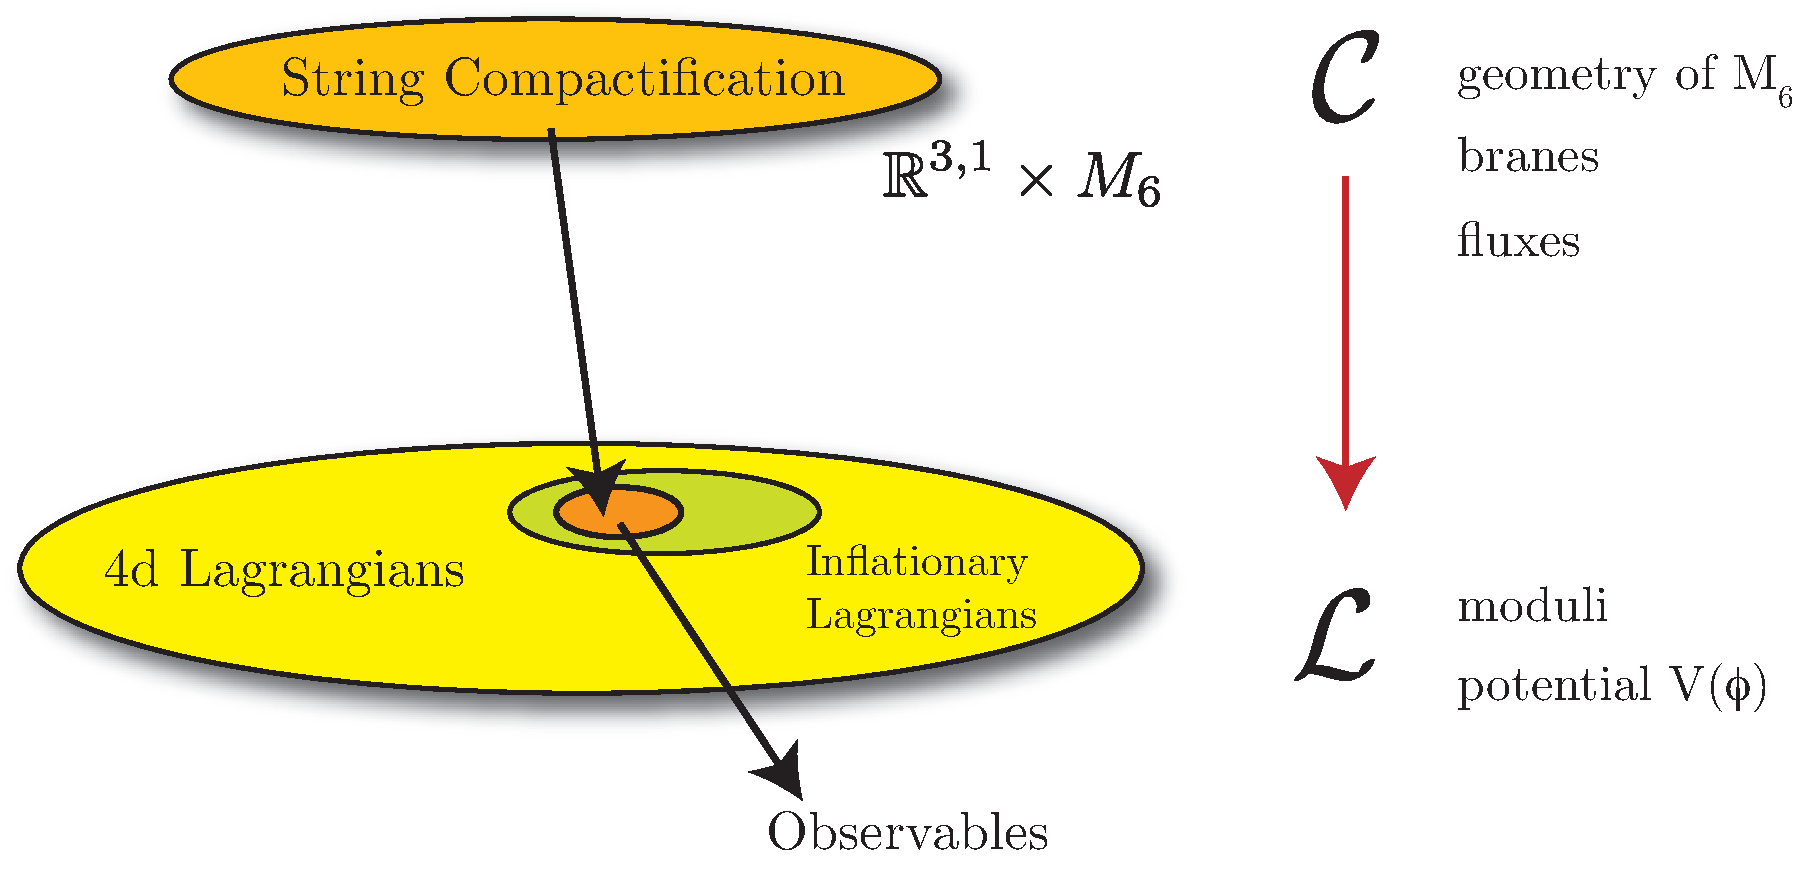
\includegraphics[width=.8\textwidth]{Philosophy}
%\vspace{-0.5cm}
\caption{10次元のコンパクト化データから4次元の作用へ．}
\label{fig:10}
\end{figure}

\subsubsection{弦コンパクト化の構成要素}

弦の量子論は4次元を超える時空次元で自然に定義され，余分な空間次元をコンパクト化すると4次元の物理が現れることはよく知られている．具体的には，臨界10次元IIB型弦理論を6次元カラビ--ヤウ空間上にコンパクト化する場合に焦点を絞る．\footnote{この用語に馴染みのない読者には，文献~\cite{Hertzberg:2007ke}にある弦理論用語から普通の英語への辞書が役立つだろう．}
% (to be precise, our compactifications will only be conformal to spaces that are well-approximated by orientifolds of Calabi-Yau manifolds, but we will not need this fine point.)

この種類に属する膨大な数の異なるコンパクト化は，位相，幾何，および量子化されたフラックスや巻き付いたDブレーンなどの離散的データによって区別される．
弦理論の模型構築における中心的な課題は，10次元の源が4次元有効理論をどのように決定するかを詳細に理解することである（図~\ref{fig:10}参照）．
10次元のコンパクト化データを ${\cal C}$ と表すと，この手順は模式的に
\beq
\label{equ:S10S4}
{\cal S}_{10}[{\cal C}] \quad \to \quad  {\cal S}_4\, .
\eeq
異なるコンパクト化データ ${\cal C}$ からは，場の内容，運動項，スカラー・ポテンシャル，対称性の性質がさまざまに異なる多数の4次元有効理論 ${\cal S}_4$ が生じる（これが弦理論の解の{\it ランドスケープ}である）．
可能なデータ ${\cal C}$ の空間と式~(\ref{equ:S10S4}) の写像の性質を理解することで，興味深い4次元の物理を生むコンパクト化を特定し，さらには分類できるかもしれない．


\begin{figure}[h!]
	\centering

\includegraphics[width=.4\textwidth]{FluxCompactification}
%\vspace{-0.5cm}
\caption{フラックス・コンパクト化の構成要素：フラックスと巻き付いたブレーン．}
\label{fig:flux}
\end{figure}

\subsubsection{インフラトンの有効作用}

われわれの目的にとって，有効理論の最も重要な自由度は4次元スカラー場である．{\it モジュライ}として知られるスカラー場は，コンパクト化多様体の変形から生じ，ここで考えるカラビ--ヤウ空間では通常数百個に上る．また，存在するDブレーンの位置，向き，およびゲージ場の配置からも生じる．与えられたコンパクト化データから，モジュライの運動項とスカラー・ポテンシャルを計算できる．そして，モジュライの期待値が4次元有効理論のパラメータを決める．Dブレーンや量子化されたフラックスのような一般的な10次元のエネルギー運動量源があると，コンパクト化を変形するにはエネルギーが必要となり，多くの（ただし必ずしもすべてではない）モジュライ場が質量を獲得する~\cite{Douglas:2006es}．

${\cal S}_4$ に現れるスカラー場を，質量がハッブル・スケールより小さい軽い場 $\phi,\psi$（$m_\phi, m_\psi \ll H$）と，質量がハッブル・スケールよりはるかに大きい重い場 $\chi$（$m_\chi \gg H$）に分けると便利である．ここで，軽い場の一つを $\phi$ と記し，インフラトン候補と同定する．

適切なインフレーションが生じうるかを理解するには，重い場も軽い場も含め，すべてのスカラー場を理解しなければならない．まず，十分に重いモジュライ場はインフレーション中に事実上凍結しているため，それらを積分消去し，軽い場だけの有効作用を得るべきである：
\beq
{\cal S}_4(\phi, \psi, \chi) \quad \to \quad {\cal S}_{4, \rm eff}(\phi,\psi)\, .
\eeq
これらの重いモードの積分消去は一般に，インフラトン候補のポテンシャルに寄与を誘起する．すなわち，{\it モジュライ安定化はeta問題に寄与する}．
これは，\S\ref{sec:eft}の有効場理論の議論で高次元演算子による補正が現れたことと，完全に類似している．

次に，インフラトン以外のスカラー場もインフレーション中に軽ければ，通常それらはダイナミクスに重要な影響を及ぼすため，質量 $m_\psi \ll H$ をもつすべての場 $\psi$ の発展を調べるべきである．さらに，結果として生じる多場インフレーションのダイナミクスが適切であっても，軽い自由度は後期宇宙論で問題を引き起こしうる．軽いスカラー場はインフレーション中にエネルギーを吸収し，インフレーション後も存在し続ければ，ビッグバン元素合成の最中またはその後にこのエネルギーを放出して，軽元素存在量についての成功した予測を損なう可能性がある．また，軽いモジュライは重力程度の強さの第5の力を媒介するため，現在の宇宙でも問題になる．これらの後期の問題を避けるには，$m_\psi \gg 30 ~\rm{TeV}$ を保証すれば十分である．この場合，モジュライはビッグバン元素合成の前に崩壊する．簡単化のため，インフラトン以外のすべての場が $m \gg H$ を満たすと仮定することもあるが，これは物理的に必須ではない．インフレーション中の有効理論がただ一つの自由度だけをもつようにするための仮定にすぎない．



\subsectionlink{{\sl 事例研究：}ワープしたDブレーン・インフレーション}
\label{sec:warped}

弦理論のインフレーション模型では，インフラトン・ポテンシャルに寄与する演算子を列挙でき，原理的にはその係数さえも与えられたコンパクト化データによって計算できる．
これらの問題を具体的に示すには，特定の模型を詳しく調べると有用である．
そこで以下では，比較的よく理解されている小場インフレーション模型である，{\it{ワープしたDブレーン・インフレーション}}を事例として取り上げる．

\subsubsection{ワープしたスロート幾何におけるD3ブレーン}

このシナリオでは，安定化されたコンパクト空間のワープしたスロート領域内でのD3ブレーンの運動がインフレーションを駆動する~\cite{KKLMMT}．
4次元のローレンツ（またはド・ジッター）不変性を保つため，D3ブレーンはわれわれの4次元時空を満たし，余剰次元内では点状である（図~\ref{fig:throat}参照）．
\begin{figure}[h!]
	\centering
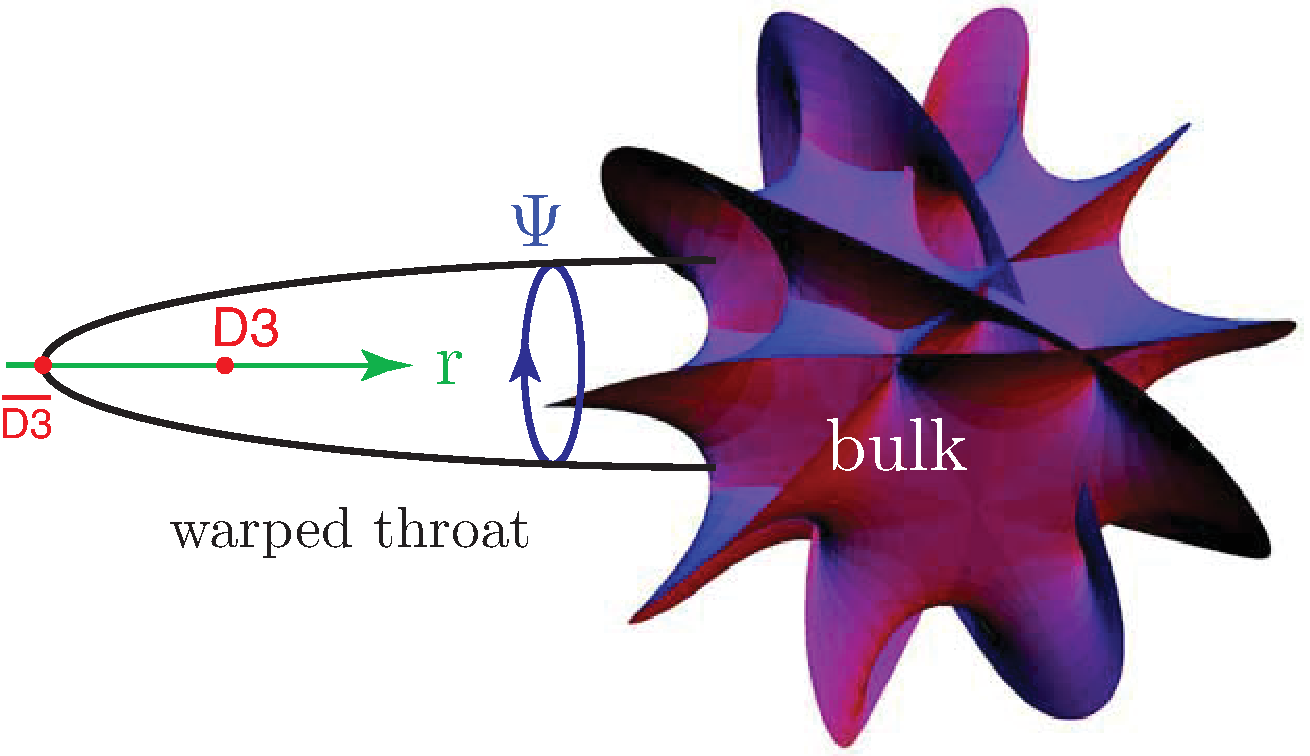
\includegraphics[width=.65\textwidth]{KKLMMT}
%\vspace{-0.5cm}
\caption{ワープしたスロート幾何におけるD3ブレーン・インフレーション．D3ブレーンは4次元時空を満たすため，余剰次元内では点状である．円は角度座標 $\Psi$ をもつ底多様体 $X_5$ を表す．ブレーンは動径方向 $r$ に運動する．$r_{\rm UV}$ でスロートはコンパクトなカラビ--ヤウ空間につながる．反D3ブレーンは，スロートの先端 $r_{\rm IR}$ でエネルギーを最小にする．}
\label{fig:throat}
\end{figure}
コンパクト化の大域的構造は，4次元時空（計量 $g_{\mu \nu}$）とカラビ--ヤウ空間に共形な空間とのワープ積であると仮定する：
\beq
\label{equ:metric}
\d s^2 = e^{2A(y)} g_{\mu \nu} \d x^\mu \d x^\nu + e^{-2A(y)} g_{mn} \d y^m \d y^n \, ,
\eeq
ここで $g_{mn}$ はカラビ--ヤウ計量であり，ある領域では5次元アインシュタイン多様体 $X_5$ 上の錐として近似できる：
\beq
g_{mn} \d y^m \d y^n = \d r^2 +r^2 \d s_{X_5}^2\, .
\eeq
このようなスロート領域の典型例がKlebanov--Strassler（KS）幾何である~\cite{KS}．この場合，$X_5$ は $\Bigl(SU(2)\times SU(2)\Bigr)/U(1)$ の剰余空間 $T^{1,1}$ であり，スロートの先端 $r=0$ に生じるはずの錐特異点は，適切なフラックスの存在によって滑らかになる．
したがって，スロートの先端は有限の動径座標 $r_{\rm IR}$ に位置し，一方 $r=r_{\rm UV}$ でスロートはワープしていないバルク幾何に接続される．
関連する領域 $r_{\rm IR} \ll r < r_{\rm UV}$ では，ワープ因子は次のように書ける~\cite{KT}：
\beq
\label{equ:warp}
e^{-4A(r)} = \frac{R^4}{r^4} \ln \frac{r}{r_{\rm IR}}\, , \qquad R^4 \equiv \frac{81}{8} (g_s M \alpha')^2\, ,
\eeq
ここで
\beq
\ln \frac{r_{\rm UV}}{r_{\rm IR}} \approx \frac{2\pi K}{3 g_s M}\, .
\eeq
ここで $M$ と $K$ はフラックス背景を指定する整数である~\cite{KS,GKP}．
% and $g_s < 1$ is the string coupling.

フラックスを源とするワープは現代のコンパクト化で一般的であり，このようなコンパクト化のモジュライの安定化の理解も大きく進んでいる~\cite{Douglas:2006es}．
したがって，現在の知識に照らせば，KSスロートを含む安定化されたコンパクト化を仮定することは妥当と思われる．


\subsubsection{場の変位範囲の限界}

インフレーション・ポテンシャルの形という複雑な問題に取り組む前に，これらの模型がそもそも大きな振幅の重力波を生みうるかを考えよう．
この問題は純粋に幾何学的な形で表すことができ，インフレーションのダイナミクスの詳細には依存しないことがわかる~\cite{Baumann:2006cd}．
Lyth限界から，大きな重力波信号には超プランク的な場の変位が必要であることがわかっている．そこで最小限の要請として，ワープしたDブレーン・インフレーションで超プランク的な場の値に到達できるかを問う．

インフラトンの運動項はプローブD3ブレーンのDirac--Born--Infeld（DBI）作用によって決まり，正準的なインフラトン場は動径座標の定数倍と同定される：$\phi^2 \equiv T_3 r^2$．ここで $T_3 \equiv \left[(2\pi)^3 g_s \alpha'^2 \right]^{-1}$ はD3ブレーンの張力であり，$g_s$ は弦結合，$2\pi\alpha'$ は弦の張力の逆数である．
スロートの長さ $\Delta r = r_{\rm UV} - r_{\rm IR} \approx r_{\rm UV}$ は，インフラトン場の変位の上限を与える：
\beq
\Delta \phi^2 \ < \ T_3\, r_{\rm UV}^2\, .
\eeq
素朴には，スロートの長さを増やすだけで，これをいくらでも大きくできるように思える．しかしそうするとコンパクト空間の体積が変わり，インフラトンの変位を測る単位である4次元プランク質量にも影響する．
この効果を考慮するため，次元縮約によって4次元プランク質量 $\Mp$ と10次元重力結合 $\kappa_{10}^2 = \frac{1}{2} (2\pi)^7 g_s^2 (\alpha')^4$ が次のように関係づけられることに注目する：
\beq
\Mp^2 = \frac{V_6}{\kappa_{10}^2}\, ,
\eeq
ここで $V_6 \equiv \int \d^6 y \sqrt{g} e^{2A(y)}$ は内部空間の（ワープした）体積である．$\Delta \phi/\Mp$ の上限を求めたいので，スロート領域の体積を用いて $V_6$ に下限を与える（バルク体積の見積もりも含めれば，結論はさらに強まるだけである）：
\beq
V_6 \ > \ (V_6)_{\rm throat} = {\rm Vol}(X_5) \int_0^{r_{\rm UV}} \d r \, r^5 e^{2A(r)} = 2\pi^4 g_s N (\alpha')^2 r_{\rm UV}^2\, ,
\eeq
ここで $N \equiv M K$ は背景フラックスの大きさを表す．超重力近似を制御するには（また背景に十分なワープを実現するには），$N \gg 1$ が必要である．
以上を組み合わせると，次を得る~\cite{Baumann:2006cd}：
\beq
\fbox{$\displaystyle
\frac{\Delta \phi}{\Mp} \ < \ \frac{2}{\sqrt{N}} $} \, .
\eeq
$N \gg 1$ なので，インフラトンの変位は常にプランク・スケール未満，$\Delta \phi \ll \Mp$ であり，重力波の振幅は必然的に小さい．
この議論が純粋に幾何学的で，次に論じるインフレーション・ポテンシャルの複雑な詳細には依存しなかったことを，再び強調しておく．

\subsubsection{D3ブレーンのポテンシャル}
\label{sec:gravity}

インフレーションは，D3ブレーンがスロート領域の動径方向に内側へ，自然にスロートの先端に位置する反D3ブレーンに向かって移動するにつれて進行する．
%The inflaton kinetic term is determined by the Dirac-Born-Infeld (DBI) action for a probe D3-brane, and leads to an identification of the canonical inflaton field with a multiple of the radial coordinate, $\phi^2 \equiv T_3 r^2$. Here, $T_3 \equiv \left[(2\pi)^3 g_s \alpha'^2 \right]^{-1}$ is the D3-brane tension, with $g_s$ the string coupling and $2\pi\alpha'$ the inverse string tension.  
接近する対の間に張られた開弦がタキオン的になって凝縮し，ブレーンが消滅すると，インフレーションが終わる．


この単純化した描像では，インフレーションはブレーン・反ブレーン対の極めて弱い（ワープによって抑制された）クーロン相互作用により駆動される~\cite{KKLMMT}．しかし実際はもっと複雑である．モジュライ安定化がインフラトン・ポテンシャルに新たな項を導入し，それらが通常クーロン項を圧倒して，より複雑なダイナミクスを駆動するためである~\cite{KKLMMT,Baumann:2006th, Baumann:2007np, Baumann:2007ah, Krause:2007jk, Baumann:2008kq}．この構図は，有効場理論の議論から予想したとおりである．モジュライ場を積分消去すると，ポテンシャルに重要な補正が誘起されると期待される．

\vskip 6pt
モジュライ安定化によって誘起される重要な補正は，\S\ref{sec:sugraETA}の超重力のF項ポテンシャルから生じるインフラトン質量項である．F項ポテンシャル，すなわちモジュライを含む超ポテンシャル項によって安定化された真空では，質量項 $H^2_0 \phi^2 = \frac{1}{3} V_0(\phi_\star) \frac{\phi^2}{M_{\rm pl}^2}$ が得られる~\cite{KKLMMT}．
ここで $\phi_\star$ はインフラトン場の任意の基準値であり，パラメータ $H_0$ を現在のハッブル定数と混同してはならない．

しかし，コンパクト化における超対称性を破る追加効果など，ほかのさまざまな起源からもポテンシャルへの寄与が予想される~\cite{Baumann:2008kq}．クーロン相互作用 $V_{0}(\phi)$ と質量項 $H_0^2 \phi^2$ 以外のポテンシャルへのすべての寄与をまとめて $\Delta V(\phi)$ と定義しよう．すると，全ポテンシャルとそれに伴うetaパラメータへの寄与は次のように書ける：
\begin{eqnarray}
\label{equ:Vphi}
V(\phi) &=& V_{0}(\phi) \ \, + \ H^2_0 \phi^2 \ + \ \Delta V(\phi) \\
\eta_{\rm v}(\phi) &=& \quad \eta_0 \quad +  \quad\frac{2}{3} \ \ \ \ + \  \Delta \eta_{\rm v}(\phi) \quad = \quad  ?
\end{eqnarray}
ここで，クーロン相互作用は非常に弱いため $\eta_0\ll 1$ である．
（より一般には，$V(\phi)$ のうち $\eta$ への寄与が無視できるすべての項を $V_0(\phi)$ と{\it 定義}できる．これにはブレーン・反ブレーン間のクーロン相互作用だけでなく，例えば宇宙定数へのバルクからの寄与など，ほぼ一定のエネルギーのほかの起源も含められる．）

明らかに，$\eta_{\rm v}$ が小さくなりうるのは，$\Delta V$ が式~(\ref{equ:Vphi}) の質量項を相殺できる場合に限られる．したがって，$\Delta V$ への関連するすべての寄与を列挙し，どのような状況で近似的な相殺が起こりうるかを理解しなければならない．ほかの寄与を知らないまま $\Delta V$ への一部の寄与だけを特定しても不十分であることに注意しよう．

ワープしたDブレーン・インフレーションが理論的に大きな注目を集めてきた理由の一つは，計算可能性が高いことである．ごく一般に，曲率が小さく弦結合が弱い，明示的で安定化されたコンパクト化の全データが得られれば，注意深く次元縮約を行うことにより，原理的にはDブレーン・インフラトンのポテンシャルを任意の精度まで計算できる．一般のコンパクトなカラビ--ヤウ空間でこれが現在不可能なのは，二つの理由による．一般のカラビ--ヤウ空間について計量データがほとんど得られていないことと，モジュライ安定化が完全に明示された例がまれなことである．

しかし，十分に長いスロートは{\it 非コンパクトな}スロート幾何（すなわち無限に長いスロート）でよく近似でき，そのカラビ--ヤウ計量はしばしば求められる．重要な例が，完全に明示的で至る所滑らかなKlebanov--Strassler解~\cite{KS}である．完全な計量データがあると，少なくともまだ安定化されていないコンパクト化の段階では，プローブDブレーンのダイナミクスの研究が大幅に容易になる．
さらにこれから，モジュライ安定化とスロートの有限の長さの効果を系統的に取り込む方法を説明する．この方法では，D3ブレーンが運動するスロートを記述する超重力解の摂動を調べる．具体的にはKSスロートを例として扱うが，方法自体ははるかに一般的である．
この扱いによって，式~(\ref{equ:Vphi}) の補正項 $\Delta V$ を明示的に表し，モジュライ安定化がある場合のインフレーションの特徴を取り出せる．

\subsubsection{超重力による解析の概要}

以下では，ワープしたD3ブレーン・インフレーションのインフラトン・ポテンシャルの計算を説明する．
これは完全なポテンシャルを理解するうえでの課題の雰囲気を示すためだけのものである．詳細については文献~\cite{KKLMMT, Baumann:2006th, Baumann:2007ah, Baumann:2008kq, Baumann:2007np}を参照されたい．

IIB型弦理論は，ディラトン，$p$形式フラックス，ワープ因子，計量摂動などの名で呼ばれる十数個の場を含む．原理的には，これらすべての場がインフラトン自由度に結合する可能性を考慮し，望む精度でインフラトン・ポテンシャルを計算する際に取り込まなければならない．
しかしD3ブレーンは特別であり，ワープ因子と5形式フラックスの特定の組合せだけに結合し，ほかのすべての場の摂動には反応しない：
\beq
V_{\rm D3}(\phi) = T_3 (e^{4A} - \alpha)\ \equiv T_3 \Phi_-\, ,
\eeq
ここでスカラー関数 $\alpha(\phi)$ は5形式フラックス $F_5$ に関係している．
したがって，関心の対象は $\Phi_- =  e^{4A}-\alpha$ という量の摂動である．
KS背景では $\Phi_- $ はゼロだが，スロートとバルク幾何の結合，および巻き付いたD7ブレーンなどのモジュライを安定化する自由度との相互作用により，ゼロでない $\Phi_-$ が誘起される．誘起された $\Phi_-$ の摂動を調べるため，超重力の運動方程式を考察する：
\beq
\label{equ:Phim}
\fbox{$\displaystyle
\nabla^2 \Phi_- = \frac{1}{24} |{\cal G}_-|^2 + R $}\, ,
\eeq
ここで ${\cal G}_-$ は3形式フラックスの特別な（虚反自己双対な）組合せであり，$R$ は4次元のリッチ・スカラーである．
インフレーション中の $R$ は，ハッブル・パラメータ $H$ の2乗で与えられる．

すべての場は5次元の底多様体 $X_5 = T_{1,1}$ 上での調和展開として表される．例えば，
\beq
\Phi_-(\phi, \Psi) = \sum_{LM} \Phi_{LM} \left( \frac{\phi}{\phi_{\rm UV}} \right)^{\Delta(L)} Y_{LM}(\Psi) + c.c.\, ,
\eeq
ここで $\Psi$ は $T_{1,1}$ 上の五つの角度をパラメータ化し，スケーリング次元 $\Delta$ は角方向のラプラシアンの固有値によって決まる．
したがって固有値スペクトルが，補正項の動径方向のスケーリングを決定する．

\begin{enumerate}
\item {\it 斉次解}

斉次方程式
\beq
\nabla^2 \Phi_- = 0\, ,
\eeq
の解は文献~\cite{Baumann:2008kq}で求められた．主要な補正の動径方向のスケーリングは次のとおりである：
\beq
\Delta \ = \ \frac{3}{2}\, , \, 2 \, ,  \ \cdots \ .
\eeq

\item {\it 非斉次解}
\begin{enumerate}
\item {\it 曲率が誘起する補正}

4次元ド・ジッター時空のリッチ・スカラーはインフラトンに結合する．
これは $\Phi_-$ の運動方程式の源の項に反映される：
\beq
\nabla^2 \Phi_- =  R\, .
\eeq
$R = 12 H^2$ が一定なら，これはインフラトン質量への補正を誘起する．
これはまさにKKLMMT~\cite{KKLMMT}が見いだした，ハッブル・スケールのインフラトン質量項である．

\item {\it フラックスが誘起する補正}

虚反自己双対な3形式フラックス\footnote{ここで $\star_6$ は6次元のホッジ星演算子である．例えば文献~\cite{Nakahara}参照．} $\star_6 {\cal G}_- = - i {\cal G}_-$ も，D3ブレーンのポテンシャルへの補正の源となる~\cite{BaumannProgress}：
\beq
\nabla^2 \Phi_- = \frac{1}{24} |{\cal G}_-|^2 \, .
\eeq
${\cal G}_-$ の運動方程式 $\d {\cal G}_-= 0$ も整合的に解くと，次の主要な補正が得られる：
\beq
\Delta \ = \ 1\, , \frac{5}{2} \, ,  \ \cdots \ .
\eeq
\end{enumerate}
\end{enumerate}

以上をまとめると，式~(\ref{equ:Phim}) を解いて
%(in combination with an equation for ${\cal G}_-$) 
次が得られた~\cite{Baumann:2008kq}：
\beq
V_{\rm D3} = T_3 \Phi_- = \sum_\Delta \phi^\Delta f_\Delta(\Psi)\, ,
\eeq
ここで
\beq
\label{equ:spec}
\fbox{$\displaystyle
\Delta \ = \ 1\, , \, \frac{3}{2} \, , \, 2 \, , \, \cdots $} \ .
\eeq
インフラトン・ポテンシャルへの補正の離散的な{\it スペクトル}~(\ref{equ:spec}) が，模型の現象論を決定する．

\subsubsection{現象論的な帰結}

小さな $\phi$ において，$\Delta = \frac{3}{2}$ と $\Delta =2$ のどちらの補正が $\Delta \eta_{\rm v}$ への支配的な寄与となるかに応じて，二つの異なるシナリオが生じる（$\Delta = 1$ は $\eta_{\rm v}$ に寄与しないことに注意）：

\begin{enumerate}

\item {\it 2次の場合}

$\Delta = \frac{3}{2}$ のモードがスペクトルから射影で取り除かれるなら（これは紫外の境界条件に離散対称性を課すことで実現できる．文献~\cite{Baumann:2008kq}参照），有効な動径ポテンシャルは
\beq
V(\phi) = V_0(\phi) + \beta H^2 \phi^2\, .
\eeq
この種類のポテンシャルの現象論は，文献~\cite{KKLMMT}と~\cite{Firouzjahi:2005dh}で初めて解析的に，文献~\cite{ShanderaTye}で数値的に研究された．

\item {\it 分数べきの場合}

分数べきのモード $\Delta = \frac{3}{2} $ が存在すると，変曲点模型が導かれる~\cite{Baumann:2008kq, Baumann:2007ah, Baumann:2007np, Krause:2007jk}（図~\ref{fig:fractional}参照）．

\begin{figure}[h!]
	\centering
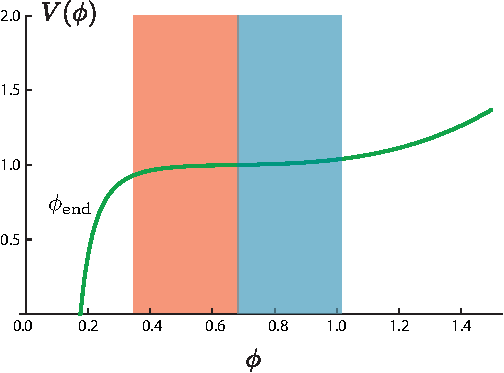
\includegraphics[width=.55\textwidth]{Fractional}
%\vspace{-0.5cm}
\caption{変曲点インフレーション．}
\label{fig:fractional}
\end{figure}



\end{enumerate}


\subsubsection{まとめと展望}
\label{sec:perspective}

\S\ref{sec:eft}では，eta問題が次元6のプランク・スケールで抑制された演算子にどのように敏感であるかを説明した．
インフレーションの有効場理論模型では，寄与する補正項の相殺によるeta問題の解決を，もちろん常に{\it 仮定}できる．言い換えれば，次元6のプランク・スケールで抑制された補正の間で近似的な相殺が起こり，平坦なポテンシャル $V(\phi)$ が生じると仮定できる．
弦理論のインフレーション模型でこの道を選ぶことは，プランク・スケールで抑制された寄与を，弦理論をのぞく（限られた）窓として用いる機会を放棄することである．さらに，いったん $\phi$ を弦コンパクト化の物理的自由度と同定すれば，ポテンシャルの正確な形は原理的にはコンパクト化の残りのデータによって完全に指定される．（この段階で解析に推測を混ぜ込むと，実質的に「弦理論から導出された」シナリオが「弦理論に着想を得た」シナリオに変わってしまう．後者は宇宙論的模型としては興味深くても，弦理論の理解には寄与しない．）
したがって，eta問題の克服は詳細な計算の問題となる．原理的には完全な
ポテンシャルを第一原理から計算でき，実際にも多くの場合， %at least
最低次のポテンシャルへの補正を分類できる．

本節では，ワープしたDブレーン・インフレーションの主要な補正を列挙し，偶然の相殺（または微調整）によって，限られたインフラトンの値の範囲でetaを小さくできることを示した．
これは，D3ブレーンをもつワープしたスロート模型にインフレーション解が存在することの非自明な証明を与える．


\subsectionlink{{\sl 事例研究：}アクシオン・モノドロミー・インフレーション}
\label{sec:LargeField} 

次に，第2の事例研究として，弦理論における大場インフレーションの例に移る．
\S\ref{sec:EFT}で論じたように，これらの模型の特有の課題は，プランク・スケールに近い質量をもつ自由度とインフラトンとの結合から生じる，インフラトン・ポテンシャルへの寄与の無限級数を制御しなければならないことである．これらの項を直接列挙して微調整すること（\S\ref{sec:warped}の小場の例で行ったこと）は明らかに非現実的であり，これらの項を制御または禁止する対称性の議論を構築することが不可欠と思われる．

この方向で影響力のある提案が自然インフレーション~\cite{Freese:1990rb}（{\bf 第1講}参照）であり，そこでは擬南部--ゴールドストーン粒子（すなわちアクシオン）がインフラトンである．摂動論的には，アクシオン場 $a$ は連続シフト対称性 $a\to a+const $ をもつが，これは非摂動効果によって離散対称性 $a\to a+2\pi$ へと破れる．
非摂動効果は周期的なポテンシャルを生成する：
\begin{equation}
V(\phi)=\frac{\Lambda^4}{2} \left[ 1- \cos \left({\phi \over f}\right) \right]+ \ldots\, ,
\end{equation}
ここで $\Lambda$ は力学的に生成されるスケール，$f$ はアクシオン崩壊定数と呼ばれる量であり，$\phi \equiv  a f$ である．省略した項は高調波である．
%The reader can easily verify from Eq.~(\ref{equ:SR}) that if the omitted terms are negligible and $f>M_{\rm pl}$, this potential can drive prolonged inflation.

上で説明したように，シフト対称性によって超プランク的な場の変位範囲が保護される有効理論を提案する際には，その構造に紫外完備化が存在するかが重要な問題となる．したがって，弦理論において崩壊定数 $f>M_{\rm pl}$ をもつアクシオンを探すべきである．


\subsubsection{弦理論におけるアクシオン}

\subsubsection*{$p$形式から生じるアクシオン}

弦コンパクト化には多くのアクシオンが存在し，コンパクト空間の $p$サイクル上で $p$形式ゲージ・ポテンシャルを積分することによって生じる．例えばIIB型弦理論では，Neveu--Schwarz（NS）2形式 $B$ を2サイクル $\Sigma_i$ 上で積分して得られるアクシオン $b_i =2\pi \int_{\Sigma_i} B$ と，Ramond--Ramond（RR）2形式 $C$ から得られるアクシオン $c_i =2\pi \int_{\Sigma_i} C$ がある．
フラックスや，巻き付いて時空を満たすブレーンのような追加要素がなければ，これらのアクシオンのポテンシャルは古典的に平坦であり，10次元作用のゲージ不変性に由来する連続シフト対称性をもつ．インスタントン効果はこの対称性を離散部分群 $b_i \to b_i + 2\pi$（$c_i \to c_i + 2\pi$）へと破る．
これによってアクシオン・ポテンシャルに周期的な寄与が生じる．その周期をこれから見積もる．
弦理論の既知の計算可能な極限では，アクシオン崩壊定数は $M_{\rm pl}$ より小さいことがわかる~\cite{Banks:2003sx,Svrcek:2006yi}．弦コンパクト化にあまり馴染みのない読者は，この主張を受け入れて\S\ref{sec:axioninflation}に進んでも，話の流れを追ううえで支障はない．

\begin{figure}[h!]
	\centering
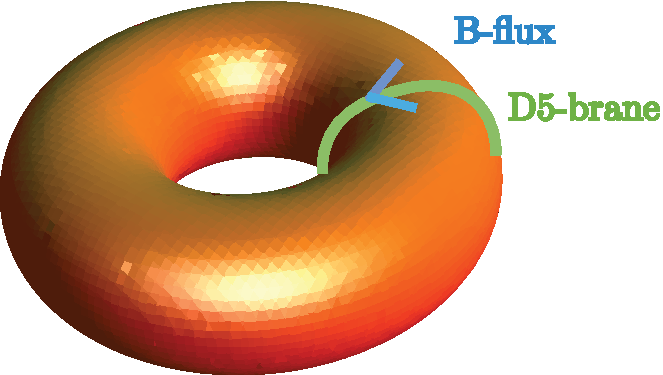
\includegraphics[width=.55\textwidth]{torus}
%\vspace{-0.5cm}
\caption{アクシオン・モノドロミー}
\label{fig:torus}
\end{figure}

\subsubsection*{弦理論におけるアクシオン崩壊定数}

コンパクト空間 $X$ 上の2形式の空間 $H^2(X, Z)$ の基底を $\omega^i$ とし，$\int_{\Sigma_i} \omega^j = \alpha'\delta_{i}^{~j}$ とする．
NS 2形式ポテンシャル $B$ は次のように展開できる：
\begin{equation}
B= \frac{1}{2\pi} \sum_i b_{i}(x)\, \omega^i\, ,
\end{equation}
ここで $x$ は4次元時空の座標である．
アクシオン崩壊定数は，その運動項の規格化から読み取れる．この場合，運動項は10次元の次の項から降りてくる：
\beq
\frac{1}{(2\pi)^7 g_s^2\alpha'^4}\int  \d^{10}x \ {1\over 2} |\d B|^2\quad \supset
\quad \frac{1}{2} \int \d^4 x \sqrt{-g}\, \gamma^{ij} (\partial^{\mu}b_i\partial_{\mu} b_j)\,
 \, ,
\eeq
ここで
\beq
\label{equ:gamma}
\gamma^{ij} \equiv \frac{1}{6 (2\pi)^9 g_s^2 \alpha'^4} \int_X \omega^i \wedge \star_6\, \omega^j\,
\eeq
であり，$\star_6$ は6次元のホッジ星演算子である．
内部空間 $X$ 上の積分を行い，場の空間の計量を $\gamma^{ij} \to f_i^2 \delta_{ij}$ と対角化することで，アクシオン崩壊定数 $f_i$ を取り出せる．

普遍的な結論を導くのは時期尚早だが，蓄積された証拠は，弦理論の計算可能な極限では得られるアクシオンの周期が常に $M_{\rm pl}$ より小さいことを示唆している~\cite{Banks:2003sx,Svrcek:2006yi}．
これは議論に不可欠なので，簡単な例で示そう．コンパクト化が等方的で，典型的な長さスケールが $L$，体積が $L^6$ であると仮定する．このとき
\beq \alpha' M_{\rm pl}^{2}= \frac{2}{(2\pi)^7}\frac{L^6}{g_s^2\alpha'^3} \eeq
を用いると，式~(\ref{equ:gamma}) から
\begin{equation}
f^2\approx M_{\rm pl}^2\, \frac{\alpha'^2}{6(2\pi)^2 L^4}\, .
\end{equation}
制御可能なコンパクト化では $L \gg \sqrt{\alpha'}$ が必要なので，$f \ll M_{\rm pl}$ となる．
はるかに一般的な配置でも，定性的に同様の結論が成り立つ~\cite{Banks:2003sx,Svrcek:2006yi}．

\subsubsection{弦理論におけるアクシオン・インフレーション}
\label{sec:axioninflation}

上の結果は，単一のアクシオン場による自然インフレーションが，既知の弦コンパクト化では実現できないことを意味するように見える．弦理論は多くのアクシオンを与えるが，十分に広い場の変位範囲をもつものは一つもない．しかし，この障害を回避するための妥当な提案が少なくとも二つある．

\subsubsection*{Nフレーション}

最初の提案は，数百個ものアクシオンの集団励起が，インフレーションに十分な有効な場の変位範囲をもちうるというものであった~\cite{Nflation, Easther:2005zr}．
インフラトンの役割は，集団場
\beq
\phi^2 = \sum_{i=1}^N \phi_i^2\, .
\eeq
個々の場の変位範囲がプランク・スケール未満，$\phi_i < M_{\rm pl}$ であっても，場の数 $N$ が十分に大きければ，有効場 $\phi$ は超プランク的な変位をもちうる．
この「Nフレーション」の提案は補助インフレーション~\cite{Liddle:1998jc}の具体例だが，特に重要なのは，インフレーションを妨げる補正からアクシオン・ポテンシャルを保護するうえで，対称性が役立つことである．有望ではあるものの，このシナリオの原理実証はまだなされていない．多数の軽い場が存在すると，ニュートン定数に問題となる繰り込みが生じ，その結果として有効な場の変位範囲が狭くなるためである．
Nフレーションの最近の研究については，文献~\cite{Kallosh:2007cc, Grimm:2007hs}参照．


\subsubsection*{アクシオン・モノドロミー}

ここでは代わりに，一つの周期的なアクシオン場が何周もする間インフレーションが続くことを可能にする，基本的な機構である{\it{モノドロミー}}を説明する．（素朴な）配置空間の閉じたループに沿って輸送したとき，系が新しい配置に到達するなら，その系はモノドロミーをもつという．典型例は螺旋階段である．素朴な配置空間は角度座標で記述されるが，$2\pi$ だけ移動すると系は変化する．（実際，この簡単な模型は，アクシオン・モノドロミー・インフレーションのポテンシャルを非常によく記述することがわかる．）
モノドロミーを用いて弦理論で制御可能な大場インフレーションを実現するという考えは，Silverstein と Westphal~\cite{Silverstein:2008sg}によって初めて提案された．彼らは，ニル多様体の内部に巻き付いたD4ブレーンを含む模型を論じた．本節では，その後に提案された文献~\cite{MSW}のアクシオン・モノドロミーに焦点を当てる．この場合，アクシオンによってパラメータ化された場の空間の円に沿って輸送すると，4次元のポテンシャル・エネルギーにモノドロミーが生じる．

このようなモノドロミーはさまざまなコンパクト化で可能だが，ここでは一つの具体例に集中する．カラビ--ヤウ・オリエンティフォールド上のIIB型弦理論を考えよう．これは世界面の向きの反転と幾何学的な対合を含む離散対称性によって，カラビ--ヤウ多様体の商を取ったものである．具体的には，対合は固定点と固定4サイクルをもち，それらはそれぞれO3プレーンとO7プレーンとして知られていると仮定する．さらにコンパクト化が，適切な2サイクル $\Sigma$ に巻き付き時空を満たすD5ブレーンを含むなら，アクシオン $b=2\pi \int_{\Sigma}B$ はポテンシャル・エネルギーにモノドロミーを示しうる．（同様に，巻き付いたNS5ブレーンはアクシオン $c=2\pi \int_{\Sigma}C$ にモノドロミーを生じさせる．）
言い換えれば，$\Sigma$ に巻き付くD5ブレーンのポテンシャル・エネルギーは，アクシオンの周期関数では{\it ない}．巻き付いたブレーンの存在によってアクシオン作用のシフト対称性が破れるからである．実際，$b$ の増加とともにポテンシャル・エネルギーは際限なく増大する．

D5ブレーンの場合，問題のポテンシャルは，巻き付いたDブレーンのDirac--Born--Infeld作用から生じる：
\begin{eqnarray}
S_{\rm DBI} &=& \frac{1}{(2\pi)^5 g_s \alpha'^3} \int_{{\cal M}_4 \times \Sigma}  \d^6 \xi \, \sqrt{\det(G+B)} \\
&=& \frac{1}{(2\pi)^6 g_s \alpha'^2} \int_{{\cal M}_4} \hskip -6pt \d^4 x\, \sqrt{-g} \, \sqrt{(2\pi)^2\ell_\Sigma^4 + b^2} \label{equ:bb}\, ,
\end{eqnarray}
ここで $\ell_\Sigma$ は弦単位で測った2サイクル $\Sigma$ の大きさである．
式~(\ref{equ:bb}) のブレーン・エネルギーは，シフト対称性 $b\to b +2\pi$ のもとで明らかに不変ではない．ただし，この対称性は，巻き付いたD5ブレーンを取り除いた対応するコンパクト化の対称性である．このように，DBI作用は $b$ のモノドロミーを直接もたらす．さらに，$b \gg \ell_\Sigma^2$ では，ポテンシャルは正準的に規格化された場 $\varphi_b \propto b$ に対して漸近的に{\it{線形}}となる．

\vskip 6pt
この模型のインフレーションのダイナミクスは，定性的には次のとおりである．まず，曲線 $\Sigma$ に巻き付いたD5ブレーンを考え，その上の $ \int_\Sigma B$ を大きく取る．言い換えれば，アクシオン $b$ は大きな初期真空期待値をもつ．この真空期待値が減少するにつれてインフレーションが進み，最終的には $\int_\Sigma B = 0$ となり，D5ブレーンはほぼ「空」，すなわち世界体積上のフラックスがほとんどない状態となる．この過程でD5ブレーンは動かず，閉弦モジュライもほとんど変化しない．アクシオンの真空期待値が小さくなると，上で述べた漸近的に線形なポテンシャルの近似は不正確になり，ポテンシャルの曲率が無視できなくなる．式~(\ref{equ:bb}) 参照．
この段階で，アクシオンは原点のまわりに振動し始める．アクシオンと，閉弦モードまたは開弦モードであるほかの自由度との結合が，インフラトン振動からエネルギーを奪う．このエネルギーの十分な割合が最終的に可視セクターの自由度へ伝われば，高温ビッグバンが始まる．可視セクターは，例えばコンパクト化の別の場所にあるDブレーンの重なりの上に存在しうる．再加熱の詳細は標準模型の自由度とインフラトンの結合の形に強く依存しており，これはこの模型だけでなく，より一般の弦インフレーションにおいても重要な未解決問題である．
% (For representative work on reheating after string inflation, see \cite{reheating}.)


\subsubsection{コンパクト化についての考察}

アクシオン・モノドロミー・インフレーションの基本的な考えを説明したが，提案したインフレーション機構がモジュライ安定化と両立し，整合的なコンパクト化で実現できることを，なお保証しなければならない．直ちに懸念されるのは，上で特定した線形項以外にも，インフレーション中に重要な影響を及ぼすポテンシャルへの追加寄与があるかどうかである．本総説を通じて強調してきたように，インフラトン・ポテンシャルを保護する対称性がなければ，モジュライ安定化による一般的な補正が $\Delta\eta\sim {\cal O}(1)$ の寄与を与えると予想される．
したがって，インフラトン・ポテンシャルを保護する連続シフト対称性が，安定化されたコンパクト化でも適切な程度に保たれることを確認するのが不可欠である．
非摂動効果が役割を果たす特別なモジュライ安定化の場合には，シフト対称性が損なわれないことを保証するのは非常に微妙な問題となりうる．
これは文献~\cite{MSW}で詳しく説明されている．



\subsubsection{まとめと展望}
\label{sec:axionS}

Lyth限界は，観測可能な重力波信号が，インフレーション中にインフラトン場が超プランク的な距離を移動することと結びついていることを示す．
このため，大場インフレーションの有効場理論模型では，超プランク的な範囲にわたりポテンシャルの平坦性を保護するシフト対称性が必要となる．
したがって，そのようなシフト対称性が弦理論で生じ，大場インフレーションの実現に利用できるかどうかが，重要な問題となっている．

本節では，超プランク的な範囲にわたってポテンシャルを保護する，弦理論におけるシフト対称性の最初の例が得られ始めていると論じた．
モノドロミーの二重の役割を説明した．i）小さな基本領域を繰り返し通過できるようにすることで，大きな運動学的な場の範囲 $\Delta \phi > M_{\rm pl}$ を生む．ii）シフト対称性と組み合わさることで，超プランク的な範囲にわたるポテンシャルの補正を制御する．
%LM
$V$ によってごく弱くしか破れないシフト対称性は，一つの基本領域内の補正 $\Delta V$ を制御し，
%the monodromy 
さらに，ある基本領域の補正をほかのあらゆる基本領域の補正と関係づける．
したがってモノドロミーは，大場の問題を実質的に小場の問題へ還元する~\cite{Silverstein:2008sg}．

これらの模型と，それらが生じるコンパクト化を理解するにはさらに研究が必要だが，モノドロミーは弦理論において大場インフレーション，したがって観測可能な重力波信号を実現する，頑健でかなり有望な機構と思われる．



\sectionlink{今後の展望}

\subsectionlink{理論面の展望}

本講で示せたことを願うが，近年の理論的進歩は目覚ましい．10年前には弦理論と宇宙論を結びつける提案はわずかしかなく，モジュライを安定化する問題にもまだ取り組まれていなかった．現在では弦理論を動機とする多様なインフレーション模型があり，そのうち最もよく研究された例には，モジュライ安定化についての情報が組み込まれている．さらに，弦理論におけるいくつかのインフレーション機構は，関連するすべての補正を含めてモジュライを完全に安定化しても存続するという意味で，頑健であることが示されている．

弦理論でインフレーションが可能であることを示した以外に，何が達成されたのだろうか．われわれの見方では，弦理論における明示的なインフレーション模型の主な用途は，インフレーションの量子重力に対する感度を調べる検証例，または玩具模型としての役割にある．理論面では，これらの模型は一般の場の理論におけるインフレーションの実現でeta問題が重要であることを強調し，場の理論では不自然に見えても弦理論では自然と思われるインフレーション機構を導き，原始テンソルモードの検出がもつ意味についての理解を明確にしてきた．

今後の理論的進歩の方向を予測するのはもちろん難しい．特に，弦理論における予見できない根本的な進歩によって，インフレーション模型構築に使える道具が増えることが期待されるからである．
しかし，モジュライ安定化がさらに着実に進歩し，すべてのモジュライが安定化された明示的な例が追加されると予想してよいだろう．そのようなコンパクト化における完全に明示的なインフレーション模型も，間違いなく続いて現れるはずである．
現在，M理論やヘテロティック弦理論で成功した模型は少なく，穏やかな仮定のもとで，ある種のIIA型コンパクト化ではインフレーションが不可能であることが示せる~\cite{Hertzberg:2007wc, Flauger:2008ad, Caviezel:2008tf}．弦理論の一つの弱結合極限で，ほかの極限よりもインフレーションがはるかに自然だということになれば意外である．現状の差は，各極限で現在利用できるモジュライ安定化の道具の違いにも一部起因すると考えられる．より多様な弦真空でインフレーションがどのように生じうるかを理解することは，明らかに有用であろう．

弦理論で現在得られているインフレーション模型は，整合性条件（例えばタドポール相殺）と，ある程度の計算可能性の必要性から生じる，厳しい理論的制約を受ける．これらの制約は，宇宙論的観測量の間の相関，すなわち予測をもたらす．より一般的な弦コンパクト化を調べられるようになるにつれ，これらの制約の一部は間違いなく消えるだろう．しかし一部は残り，弦理論から導かれるインフレーションの有効作用の集合が，一般の場の量子論におけるインフレーションの有効作用の集合の真部分集合になることを期待できる．このような主張を確立するには，現在よりもはるかに包括的な弦コンパクト化の理解が必要であろう．



\subsectionlink{観測的な痕跡はあるか？}
\label{sec:obs}

本講で述べたインフレーションの理論的側面が興味深い大きな理由は，現在および将来の宇宙論データを用いて，実験的に{\it 検証}できることである（{\bf 第3講}参照）．

%In order to describe this connection, we will very briefly review recent achievements and near-future prospects in observational cosmology.


本講義を通じて繰り返し強調したように，インフレーションを最も劇的に確認するのは $B$モード偏光の検出であろう．それによってインフレーションのエネルギー・スケールが確立され，インフラトンが超プランク的な距離を移動したことが示される．
本講で論じたように，超プランク的な変位は，インフラトンの有効作用がプランク・スケールの物理に特に敏感となる重要な場合である．テンソル摂動が模型を判別する力の具体例として，原始重力波が検出されれば，\S\ref{sec:warped}のワープしたD3ブレーン・インフレーション・シナリオは排除される~\cite{Baumann:2006cd}．一方，上限 $r<0.07$（または $r\gg 0.07$ での検出）は，\S\ref{sec:LargeField}のアクシオン・モノドロミー・シナリオを排除する~\cite{MSW}．

さらに，単一場のスローロール・インフレーションは，多くの宇宙論的観測量について信号がないという予測をするため，別の機会も生じる．原始スカラー揺らぎは，高い精度でスケール不変，ガウス的，断熱的であると予測されるからである．したがって，非ガウス性，等曲率揺らぎ，または大きなスケール依存性（ランニング）の検出は，単一場のスローロール・インフレーションを排除する．大きな非ガウス性，非断熱性，またはスケール依存性を許すインフレーションの有効作用には，高階微分相互作用や複数の軽い場が必要となることが多く，そのような作用は弦理論ではかなり自然に生じる．本講では，インフラトン・ポテンシャルのプランク・スケールの物理に対する感度に焦点を当てたが，インフラトンの運動項も同様に紫外物理に敏感であり，弦理論は大きな非ガウス性を生みうる高階微分相互作用を理解するための有望な枠組みを与える~\cite{DBI,Alishahiha:2004eh}．

最後に，残存する宇宙ひもやほかの位相欠陥によって誘起されるCMBの温度・偏光異方性は，インフレーションの終わりまたはその後の時代の物理を探る手段となる．
宇宙ひもはブレーン・反ブレーン・インフレーションの終わりに自動的に生成され~\cite{Sarangi, CMP}，その結果生じる宇宙ひもネットワークの安定性と現象論的性質は，ワープ幾何の性質によって決まる．重力レンズ効果や特徴的な重力波バーストを通じた宇宙超ひもの検出は，胸の躍る展望である．\\

%\subsectionlink{Conclusions}


%The theoretical community will eagerly await the coming generation of experimental results \cite{Baumann:2008aq}, in the hope of extracting further clues about the physical properties of the early universe.





\newpage
\sectionlink{{\sl まとめ}：第5講}

\begingroup
\setlength{\abovedisplayskip}{5pt}
\setlength{\belowdisplayskip}{5pt}
\setlength{\abovedisplayshortskip}{3pt}
\setlength{\belowdisplayshortskip}{3pt}
近年の多くの著者による研究を通じて，弦理論における頑健なインフレーション機構が現れてきた（最近の総説については文献~\cite{BMReview, Burgess:2007pz, Kallosh:2007ig, Linde:2005dd, McAllister:2007bg, Cline:2006hu}参照）．これらの研究の主な動機は，インフレーションの有効作用が重力の紫外完備化に敏感であることと，高精度の宇宙論データを用いた実証的な検証の見通しである．

本講では，二つの例を通じて{\it インフレーションの紫外物理に対する感度}を示した：

\begin{itemize}
\item {\it eta問題}

etaパラメータ（またはインフラトン質量）の小ささは，次元6のプランク・スケールで抑制された補正に敏感である：
\beq
\Delta V \sim V \frac{\phi^2}{\Mp^2} \qquad \Rightarrow \qquad \Delta \eta_{\rm v} \sim 1\, . \nonumber
\eeq

このような項は，低エネルギー有効理論を得るために（カットオフより上の）重い自由度を積分消去すると生じる．
ワープしたブレーン・インフレーションを例として，この問題が弦理論の計算でどのように明示されるかを示した~\cite{Baumann:2006th, Baumann:2007ah, Baumann:2008kq, BaumannProgress}．

\item {\it 大場模型におけるテンソルモード}

インフレーションが観測可能な振幅の重力波を生成するには，インフラトン場が超プランク的な距離を移動する必要がある．
超プランク的な範囲にわたりインフレーション・ポテンシャルの平坦性を保護することは難しい：
\begin{itemize}
\item {\it シフト対称性がない場合}

特別な対称性がない場合，大場インフレーションのポテンシャルは，プランク・スケールで抑制された演算子の無限級数に敏感になる：
\beq
{\cal L}_{\rm eff}(\phi) = -\frac{1}{2}(\partial \phi)^2 - \frac{1}{2} m^2 \phi^2 - \frac{1}{4} \lambda \phi^4 - \sum_{p=1}^\infty \left[ \lambda_p \phi^4  + \nu_p (\partial \phi)^2    \right] \left( \frac{\phi}{M_{\rm pl}} \right)^{2p}+ \cdots \ . \nonumber
\eeq
この場合，超プランク的な範囲にわたるポテンシャルの平坦性には，多数の展開パラメータ $\lambda_p$ の微調整が必要となる（一つの質量パラメータの調整だけを必要とするeta問題と比較されたい）．

\item {\it シフト対称性がある場合}

インフラトン場がシフト対称性 $\phi \to \phi + const.$ を満たすなら，小さな係数 $\lambda_p$ をもつカオス的インフレーションの作用
 \beq
 {\cal L}_{\rm eff}(\phi) =- \frac{1}{2} (\partial \phi)^2 - \lambda_p\, \phi^p\, , \nonumber
 \eeq
は「技術的に自然」である．
\end{itemize}
したがって，検出可能な重力波を伴うインフレーション模型を構築するには，大きな運動学的範囲 $\Delta \phi > \Mp$ と，完全な弦理論で近似的に保たれるシフト対称性に保護されたポテンシャルの両方をもつ配置を，弦理論の中で見いだすことが目標となる．
このような模型は最近，文献~\cite{Silverstein:2008sg, MSW, Flauger:2009ab}で構築された．
\end{itemize}




%\newpage
%\sectionlink{{\sl Problem Set}: Lecture 4}


\endgroup
\newpage
\part{結論}


\sectionlink{{\sl 振り返り}：インフレーションに関するTASI講義}

%I showed different versions of Fig.~\ref{fig:summary} at the beginning of each of my lectures at {\sl TASI 2009}.

図~\ref{fig:summary}は，本講義で説明した重要な概念の多くをまとめている．

\begin{figure}[h!]
    \centering
        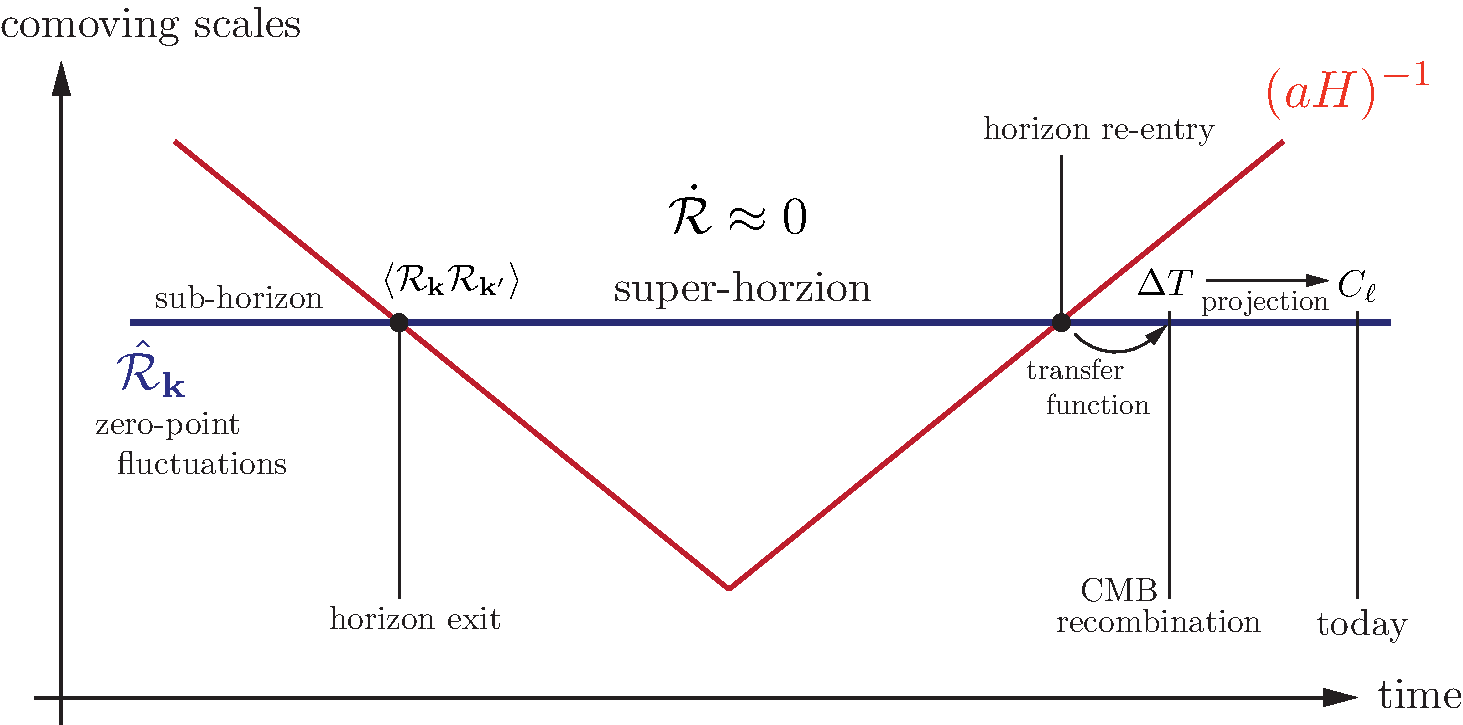
\includegraphics[width=0.9\textwidth]{summary}
    \caption{\small インフレーション宇宙における地平線の発展と摂動の生成．} % (see Figures \ref{fig:WMAP2} and \ref{fig:CMBparam}).}
    \label{fig:summary}
\end{figure} 


\begin{itemize}
\item {\bf 第1講}：インフレーションを，共動ハッブル半径 $(a H)^{-1}$ が減少する極初期宇宙の時期と定義した．この重要な特徴が地平線問題と平坦性問題の解決の核心であることを説明した．再結合時の地平線を超えるスケールで見られるCMB揺らぎの，一見すると因果性に反する相関は，それらのスケールがインフレーション中には地平線内にあり，したがって因果的につながっていたことで説明される．
\item {\bf 第2講}：モードはインフレーション中に地平線を出て，後の通常のFRW膨張期に再び地平線に入る．インフレーション中のスカラー揺らぎを，共動曲率摂動 ${\cal R}$ で記述した．${\cal R}$ の決定的な特徴は，地平線を超えるスケールで凍結し，$\dot \R \approx 0$ となることである．したがって，${\cal R}$ の初期条件はインフレーション中の地平線脱出時に計算でき，そのまま地平線への再突入時まで引き継がれる（かなり弱い仮定のもとで，これは未知の再加熱の物理に依存しない）．第2講では，地平線脱出時の曲率摂動のパワースペクトル $\langle {\cal R}_{\bf k} {\cal R}_{\bf k'} \rangle = (2\pi)^3 \delta({\bf k}+{\bf k'}) P_\R(k)$ を計算した．
\item {\bf 第3講}：地平線への再突入後，曲率摂動 ${\cal R}$ は再結合時のCMB温度の揺らぎ $\Delta T$ へと発展する．この地平線内での発展は，第3講で論じた伝達関数によって記述される．そして今日，われわれが見るのは，最終散乱面からわれわれへと投影されたCMB揺らぎである．
実験はCMB温度揺らぎの角度パワースペクトル $C_\ell$ を測定する．第3講では，観測されたCMB異方性の角度パワースペクトルを，インフレーション中に生成された原始曲率揺らぎのパワースペクトル $P_\R(k)$ に関係づける方法を説明した．
したがって，地平線内での発展を逆にたどり，投影効果を取り除くことで，CMB観測はインフレーションの摂動を探る強力な手段となる．
\item {\bf 第4講}：原始曲率摂動の3点関数 $\langle {\cal R}_{{\bf k}_1} {\cal R}_{{\bf k}_2} \R_{{\bf k}_3} \rangle = (2\pi)^3 \delta({\bf k}_1+{\bf k}_2 + {\bf k}_3) B_\R(k_1, k_2, k_3)$ は，原始揺らぎが十分に非ガウス的であれば，インフレーションの物理を探る追加の手段となる．
\end{itemize}

\sectionlink{将来の展望と未解決問題}
\label{sec:conclusion}

インフレーションに対する現在の観測的証拠を述べ，その物理をさらに検証するための将来の観測機会を取り上げた．
インフレーションを最も直接的に探る二つの手段は，原始テンソルモードと原始非ガウス性である：
\begin{itemize}
\item {\bf Bモード}

原始 $B$モード（インフレーションのテンソルモードがCMB偏光に残す痕跡）の検出は，インフレーションを確認するために可能な観測の中で，明らかに最も特徴的なものである．これによってインフレーションのエネルギー・スケールを測定し，インフラトン場が超プランク的な距離を移動したことを知ることができる．
欧州の{\sl Planck}衛星~\cite{:2006uk}，多くの地上実験や気球実験~\cite{CMBPolWorkshop, Kosowsky:2004sw, Ruhl:2004kv, Taylor:2006jw, Samtleben:2008rb, Yoon:2006jc, Oxley:2005dg, MacTavish:2007kh}，そして計画中の{\sl CMBPol}ミッション~\cite{WhitePaper, Bock:2009xw}は，いずれもインフレーション期からのこの信号の検出を目指している．理論研究者たちは，これらの実験結果を大きな期待とともに待っている．

\item {\bf 非ガウス性}

インフレーションの物理の，やや模型依存性が高い痕跡は，原始揺らぎに非ガウス性が存在する可能性である．単一場のスローロール模型では小さいと予測されるが，複数の場，高階微分相互作用，または非自明な真空状態をもつ模型は，非ガウス的な痕跡を残しうる．フーリエ空間の信号の運動量依存性は，原始揺らぎを生み出した機構を診断する強力な手段である．{\sl Planck}衛星は，原始非ガウス性を高感度で探ることになる．
\end{itemize}

本講義では，インフレーションについてかなり楽観的な見方を提示した．
これは，インフレーションの物理を理解し制約するうえで近年達成された理論・観測両面の大きな進歩を示す一方，この理論がなお直面する重要な概念的問題を省いている．ここでは，これらの理論的課題のいくつかを挙げ，詳細について関連文献を示す：
\begin{itemize}
\item {\bf 初期条件}

本講義では，インフレーションを開始するために必要な初期条件について，ごく表面的にしか触れていない．これは一部には，インフレーションの初期条件があまりよく理解されていないという事情を反映している．

単純なスローロールによるインフレーションの解析では，インフラトンの初期速度は小さく，インフラトン場の初期の非一様性はインフレーションを妨げるほど大きくないと{\it 仮定}した：

\begin{itemize}
\item {\it オーバーシュート問題}

インフレーションが起こるはずのポテンシャル領域の近くで，インフラトンの初期速度が無視できなければ，場は加速膨張を生み出すことなく，その領域を{\it 通り越してしまう}可能性がある．
この問題は小場模型でより深刻になる．そこではしばしば，場が注目する領域に到達する前にハッブル摩擦で十分に減速できないためである．

\begin{figure}[h!]
    \centering
        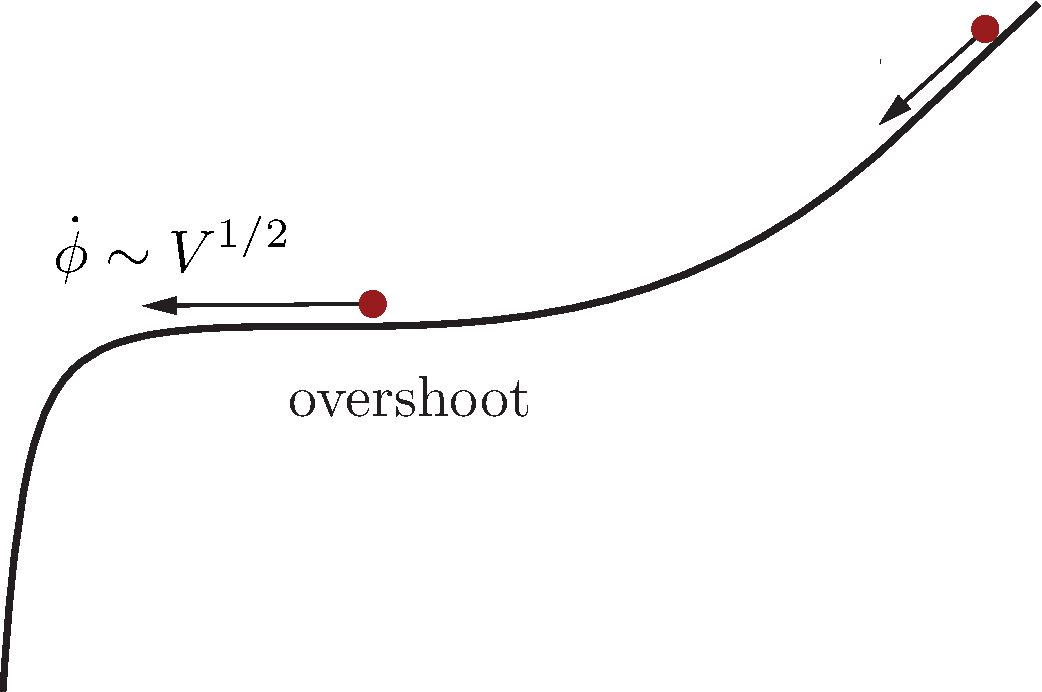
\includegraphics[width=0.38\textwidth]{overshoot}
    \caption{\small オーバーシュート問題の模式図．} % (see Figures \ref{fig:WMAP2} and \ref{fig:CMBparam}).}
    \label{fig:overshoot}
\end{figure} 



\item {\it パッチ問題}

インフラトン場の初期の非一様性は，やはり加速膨張を妨げる勾配エネルギーを与える．
具体例に対する数値解析は，インフレーションを開始するために，通常インフラトン場がその時点の地平線サイズの数倍にわたって滑らかでなければならないことを示している．

\begin{figure}[h!]
    \centering
        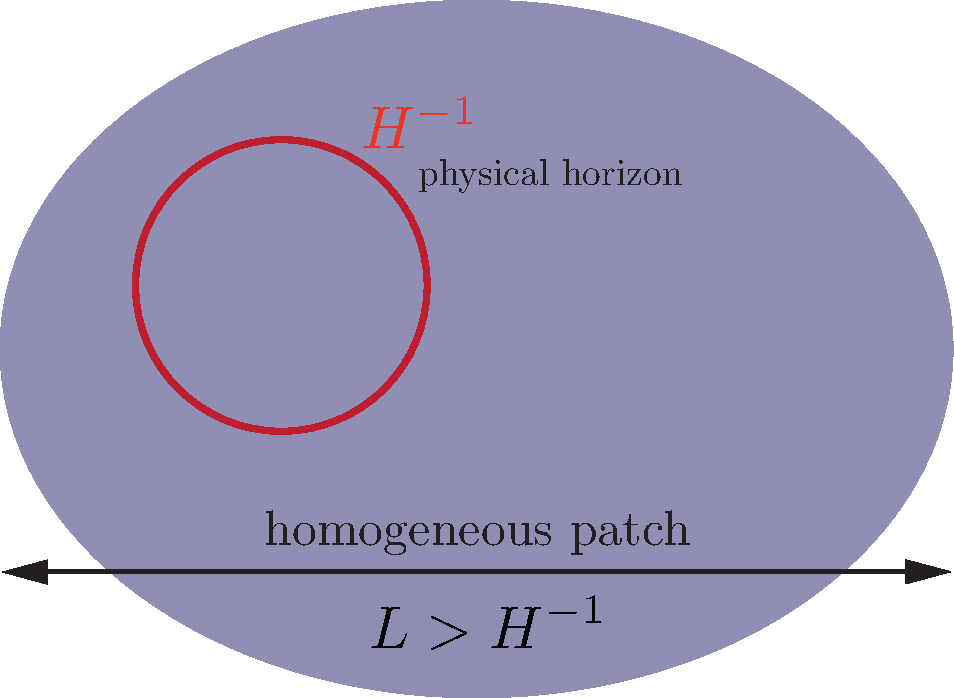
\includegraphics[width=0.38\textwidth]{patch}
    \caption{\small パッチ問題の模式図．} % (see Figures \ref{fig:WMAP2} and \ref{fig:CMBparam}).}
    \label{fig:patch}
\end{figure} 

\end{itemize}

インフレーションに必要な初期条件の微調整が実際にどれほど深刻かは，いまだ十分に理解されていない永遠のインフレーションと測度問題から切り離して論じることはできない．

\item {\bf 永遠のインフレーションと測度問題}

現代的なインフレーションの見方では，大域的にはインフレーションは決して終わらない！
インフレーションは局所的には終わり，FRW宇宙の小領域を作るが，量子揺らぎによって場が高いポテンシャル・エネルギーに保たれる領域が常に存在する．
これらの領域は指数関数的に膨張し続け，インフレーションしている領域の体積をさらに増やす．

インフレーションの初期条件がどれほど起こりやすいか，さらにはインフレーション自体が何を予測するかも，宇宙（または多宇宙）におけるインフレーションする領域としない領域の相対確率に依存する．これが測度問題である．
異なる確率測度を採用すると，インフレーションの初期条件の確率や，特定の観測的特徴（平坦性，スケール不変な揺らぎなど）をもつFRW宇宙の生じやすさが大きく変わりうる．

永遠のインフレーションと測度問題についての詳細は，文献~\cite{Vilenkin:1983xq, Linde:1986fd, Linde:1993nz, Linde:1993xx, GarciaBellido:1993wn,Vilenkin:1994ua, Garriga:2005av, Bousso:2006ev, Linde:2007nm, Bousso:2008hz, DeSimone:2008if, Garriga:2008ks, Winitzki:2008jp, Linde:2008xf}を参照されたい．

\end{itemize}

これらの問題は，インフレーションと宇宙論的初期条件に関する理論的理解を深める余地が，まだ残されていることを示している．
同時に，CMB偏光と小スケールの温度揺らぎの高精度測定の到来は，インフレーション仮説の実際の実験的検証を約束している．


\sectionlink{さらに学ぶための文献案内}

以下の教科書，総説，論文は，本講義の準備に役立ったものである．
学生諸君は，これらの文献からインフレーションについての有益な詳細をさらに学べるだろう．


\subsubsection*{教科書}

\begin{itemize}
\item Mukhanov, {\it 宇宙論の物理的基礎}

初期宇宙論と宇宙論的摂動の理論についての優れた解説．

\item Dodelson, {\it 現代宇宙論}

宇宙マイクロ波背景放射に重点を置いた，宇宙論の優れた本．非常に読みやすく，つまり寝転びながらでも読める．


\item Weinberg, {\it 宇宙論}

Steven Weinbergによる本である！

\item Liddle and Lyth, {\it 宇宙論的インフレーションと大規模構造}

インフレーション宇宙論についての包括的な概説．

\item Longair, {\it 銀河形成}

より天体物理学的な視点から見た宇宙論．

\item Birrell and Davies, {\it 曲がった時空における場の量子論}

曲がった時空における場の量子論の古典的な解説．


\end{itemize}


\subsubsection*{総説}

\begin{itemize}
\item Baumannら, {\it CMB偏光でインフレーションを探る}

CMBPolミッション概念検討のインフレーション作業部会による白書．
60人以上のインフレーションの専門家が協力して，この非常に包括的な総説を執筆した．

\item Baumann and Peiris, {\it 宇宙論的インフレーション：理論と観測}

この総説では，Hiranya Peirisと私が，専門外の読者向けにインフレーションとCMB観測の基礎をまとめた．本講義の読者には初歩的すぎるかもしれないが，就寝前の読み物を探している読者には興味深いかもしれない．

\item Baumann and McAllister, {\it 弦インフレーションの進展}

この総説では，Liam McAllisterと私が，弦理論においてインフレーションを実現するという課題を説明している．

\item Lyth and Riotto, {\it インフレーションの素粒子物理模型}

本講義で不足しているインフレーション模型の構築に関する内容は，ここで見つかる．

\item Bassettら, {\it インフレーションのダイナミクスと再加熱}

本講義で不足している再加熱に関する内容は，ここで見つかる．

\item Kinney, {\it インフレーションに関するTASI講義}

Will Kinneyによる{\sl TASI 2008}の講義は，インフレーションについて最初に読むものとして最適である．
この{\sl TASI 2009}の講義が，2番目の読み物としてよいものになっていれば幸いである．
より技術的な詳細を示すことで，Willの講義を補うよう努めた．

\item Malik and Wands, {\it 宇宙論的摂動}

1次および2次の摂動論についての優れた総説．有用な公式が多数掲載されている．


\item Komatsu, {\it 宇宙マイクロ波背景放射における非ガウス揺らぎの探究}

Eiichiro Komatsuの博士論文には，インフレーションに由来する非ガウス揺らぎについての有用な概説が含まれている．
\end{itemize}



\subsubsection*{原著論文}

インフレーションに関する原著論文の中には非常に読みやすく，一読に値するものがある：

\begin{itemize}
\item Guth, {\it インフレーション宇宙：地平線問題と平坦性問題の解となる可能性}

{\small この古典的論文はもちろん必読である．ビッグバンの謎を非常に明快に説明している．}

\item Maldacena, {\it 単一場のインフレーション模型における原始揺らぎの非ガウス的特徴}

{\small この論文は，スローロール・インフレーションの3点関数を初めて厳密に計算した．また，インフレーションの揺らぎのパワースペクトルの計算について，最も明快かつ洗練された解説の一つを与えている．本講義の扱いは，Maldacenaの論文から大きな影響を受けた．}


{\small }
\end{itemize}

\newpage


\appendix
\renewcommand{\thesection}{\Alph{section}}



\part{付録}
\sectionlink{宇宙論的摂動論}
\label{sec:CPT}
\setcounter{equation}{0}
\renewcommand{\theequation}{A.\arabic{equation}}




この付録では宇宙論的摂動論の基本事項をまとめる．内容は，Uros SeljakとChris Hirataによるプリンストン大学での講義の未公刊ノート，およびMalikとWandsの総説\cite{Malik:2008im}に基づく．

 
%\subsectionlink{Gauges and Physical Perturbations}

\subsectionlink{摂動を受けた宇宙}


%A basic assumption of cosmology is that the universe is the homogeneous and isotropic  when averaged over large scales.

一様な背景時空と宇宙のエネルギー運動量に対する摂動を考える．



\subsubsection{計量摂動}



空間的に平坦なFRW計量の最も一般的な1次摂動は
\beq
\label{equ:SVTmetric}
\d s^2 = -(1+2 \Phi) \d t^2 + 2  a(t) B_{i} \d x^i \d t + a^2(t) [(1- 2 \Psi) \delta_{ij} + 2 E_{ij}] \d x^i \d x^j 
\eeq
である．ここで，$\Phi$は\textit{ラプス}と呼ばれる3次元スカラー，$B_i$は\textit{シフト}と呼ばれる3次元ベクトル，$\Psi$は空間\textit{曲率}摂動と呼ばれる3次元スカラーであり，$E_{ij}$は空間的な\textit{せん断}を表す3次元テンソルで，対称かつトレースレス，すなわち$E^i_i = \delta^{ij} E_{ij}=0$である．時刻$t$が一定の3次元超曲面を\textit{スライス}と呼び，空間座標$x^i$を一定に保ち時間$t$のみを変化させた曲線を\textit{スレッド}と呼ぶ．



\subsubsection{エネルギー運動量の摂動}



エネルギー運動量テンソルは，密度$\rho$，圧力$p$，3次元運動量密度が消える系の4元速度$u^\mu$，および異方的応力$\Sigma^{\mu \nu}$によって記述できる．



密度摂動と圧力摂動は，自然に次のように定義される：
\beq
\delta \rho(t, x^i) \equiv \rho(t,x^i) - \bar \rho(t)\, , \qquad \text{かつ} \qquad \delta p(t, x^i) \equiv p(t, x^i) - \bar p(t)\, .
\eeq
ここで，上線は背景の値を表す．
%If it doesn't cause confusion we will often drop the overbars.

4元速度は拘束条件$g_{\mu \nu} u^\mu u^\nu = -1$を満たさなければならないため，計量を固定すると独立な成分は3つしかない．摂動された計量(\ref{equ:SVTmetric})において，摂動された4元速度は
\beq
u_\mu \equiv (-1-\Phi, a v_i) \, , \qquad \text{または} \qquad u^\mu \equiv (1 -\Phi, a^{-1}(v^i - B^i))\, .
\eeq
である．ここで$u_0$は，すべての摂動の1次まで拘束条件$u_\mu u^\mu = -1$を満たすように選んでいる．摂動のないFRW宇宙では異方的応力は消えるので，$\Sigma^{\mu \nu}$は1次摂動である．さらに，$\Sigma^{\mu \nu}$は次の拘束条件を満たす：
\beq
\Sigma^{\mu \nu} u_\nu = \Sigma^\mu_\mu = 0\, .
\eeq
$u_\mu$との直交性から$\Sigma^{0 0} = \Sigma^{0 j} = 0$が従う．すなわち，空間成分$\Sigma^{ij}$のみがゼロでない．トレースに関する条件からは$\Sigma^i_i=0$が従う．したがって，異方的応力はトレースレスな対称3次元テンソルである．



最後に，これらの定義を用いると，摂動されたエネルギー運動量テンソルは
\bea
T^0_0 &=& - (\bar \rho + \delta \rho) \\
T^0_i &=& (\bar \rho +\bar p)\, a v_i \\
T^i_0 &=& -(\bar \rho + \bar p) (v^i - B^i)/a \\
T^i_j &=& \delta^i_j (\bar p + \delta p) + \Sigma^i_j\, .
\eea
となる．エネルギー運動量テンソルに複数の寄与がある場合（例えば光子，バリオン，暗黒物質など），それらは$T_{\mu \nu} = \sum_I T^I_{\mu \nu}$と加え合わせる．このことから
\begin{eqnarray}
\delta \rho &=& \sum_I \delta \rho_I \\
\delta p &=& \sum_I \delta p_I \\
(\bar \rho + \bar p) v^i &=& \sum_I (\bar \rho_I + \bar p_I) v_I^i \\
\Sigma^{ij} &=& \sum_I \Sigma_I^{ij}\, .
\end{eqnarray}
が従う．密度，圧力，異方的応力の摂動は単純に加算される．しかし速度は加算されない．そこで3次元運動量密度を
\beq
\delta q^i \equiv (\bar \rho + \bar p) \, av^i\, ,
\eeq
と定義すると，
\beq
\delta q^i = \sum_I \delta q^i_I\, .
\eeq
となる．




\subsectionlink{スカラー，ベクトル，テンソル}



Einstein方程式は，計量摂動とエネルギー運動量の摂動を関係づける．Einstein方程式は複雑な連立2階偏微分方程式であり，しかも非線形である．幸い，平坦なFRW背景時空の対称性により，摂動を独立なスカラー，ベクトル，テンソル成分に分解できる．これによってEinstein方程式は互いに結合しない常微分方程式の組に帰着する．




\subsubsection{フーリエ空間におけるヘリシティとSVT分解}



スカラー，ベクトル，テンソル摂動への分解は，フーリエ空間で最も明快に説明できる．一般の摂動$\delta Q(t,{\bf x})$のフーリエ成分を次のように定義する：
\beq
\delta Q(t, {\bf k}) = \int \d^3 {\bf x} \, \delta Q(t,{\bf x}) e^{-i {\bf k} \cdot {\bf x}}\, . 
\eeq
まず，\underline{並進不変性}の帰結として，異なるフーリエモード（異なる波数$k$）は独立に発展することに注意する．\footnote{以下の証明はUros SeljakとChris Hirataに教えていただいた．}



\vspace{0.5cm}
\hrule \vspace{0.3cm}
{\bf 証明：}



$N$個の摂動$\delta Q_I$（$I=1,\dots, N$）について，初期時刻$t_1$から終時刻$t_2$までの線形発展を考える：
\beq
\delta Q_I(t_2, {\bf k}) = \sum_{J=1}^N \int \d^3 \bar {\bf k} \ T_{IJ}(t_2,t_1, {\bf k}, \bar {\bf k}) \delta Q_J(t_1, \bar {\bf k})\, ,
\eeq
ここで伝達行列$T_{IJ}(t_2,t_1, {\bf k}, \bar {\bf k}) $はEinstein方程式から定まり，$k$モードが混合する可能性を許している．以下では，並進不変性が実際にはそのような結合を禁じることを示す．座標変換
\beq
x^{i'} = x^i + \Delta x^i\, , \qquad \text{ただし} \quad \Delta x^i = const.
\eeq
を考える．フーリエ振幅が次のように変化することを確認できる：
\beq
\delta Q_I'(t, {\bf k} ) = e^{-i k_j \Delta x^j} \delta Q_I(t, {\bf k} ) \, .
\eeq
したがって，プライム付き座標系における発展方程式は
\begin{align}
\delta Q_I'(t_2, {\bf k}) &= \sum_{J=1}^N \int \d^3 \bar {\bf k} \ e^{-i k_j \Delta x^j} T_{IJ}(t_2,t_1, {\bf k}, \bar {\bf k}) e^{i \bar k_j \Delta x^j }\,\delta Q_J'(t_1, \bar {\bf k}) \\
&\equiv \sum_{J=1}^N \int \d^3 \bar {\bf k} \ T_{IJ}'(t_2,t_1, {\bf k}, \bar {\bf k}) \delta Q_J(t_1, \bar {\bf k})\, .
\end{align}
となる．並進不変性により，運動方程式は両座標系で同一でなければならない．すなわち，伝達行列$T_{IJ}$と$T'_{IJ}$は等しくなければならず，
\beq
 T_{IJ}(t_2,t_1, {\bf k}, \bar {\bf k}) =  e^{i(\bar k_j - k_j) \Delta x^j} T_{IJ}(t_2,t_1, {\bf k}, \bar {\bf k}) \, .
\eeq
である．これはすべての$\Delta x^j$に対して成り立たなければならない．したがって，$\bar {\bf k} = {\bf k}$であるか，あるいは$T_{IJ}(t_2,t_1; {\bf k}, \bar {\bf k}) =0$である．すなわち，波数ベクトル${\bf k}$をもつ摂動$\delta Q_I(t_2, {\bf k}) $は，波数ベクトル${\bf k}$をもつ初期摂動にのみ依存する．線形次数では，異なる$k$モードの間に結合はない．証明終．
\vspace{0.2cm} \hrule
\vspace{0.5cm}

 

次に，フーリエ波数ベクトル${\bf k}$のまわりの角度$\psi$の回転を考える．摂動をその\textit{ヘリシティ}$m$によって分類する．ヘリシティ$m$の摂動は，上の回転によって振幅が$e^{im \psi}$倍される．スカラー，ベクトル，テンソル摂動を，それぞれヘリシティ0，$\pm 1$，$\pm 2$をもつ摂動として定義する．



\vskip 6pt
波数ベクトル${\bf k}$をもつフーリエモードを考える．一般性を失わずに${\bf k}=(0,0,k)$と仮定できる（あるいは背景の回転不変性を用いてもよい）．このとき任意の摂動の空間依存性は
\beq
\delta Q \propto e^{i k x^3}\, .
\eeq
である．${\bf k}$のまわりの回転を調べるには，ヘリシティ基底
\beq
{\bf e}_\pm \equiv \frac{{\bf e}_1 \pm i {\bf e}_2}{\sqrt{2}}\, , \qquad {\bf e}_3\, ,
\eeq
に移ると便利である．ここで$\{{\bf e}_1, {\bf e}_2, {\bf e}_3\}$は直交座標基底である．第3軸のまわりの角度$\psi$の回転は，次の作用をもつ：
\beq
\left( \begin{array}{c} x^{1'}  \\ x^{2'}  \end{array}\right) = \left( \begin{array}{c c} \cos \psi & \sin \psi \\ -\sin \psi & \cos \psi \end{array}\right)  \left( \begin{array}{c} x^1 \\ x^2 \end{array}\right) \, , \qquad x^{3'} = x^3\, , 
\eeq
また，
\beq	
 {\bf e}_\pm' = e^{\pm i \psi} {\bf e}_\pm\, , \qquad {\bf e}_3' ={\bf e}_3\, .
\eeq
である．任意のテンソル$T_{i_1 i_2 \dots i_n}$の反変成分は
\beq
T'_{i_1 i_2 \dots i_n} = e^{i(n_+ -n_-)\psi} T_{i_1 i_2 \dots i_n} \equiv e^{im \psi} T_{i_1 i_2 \dots i_n}
\eeq
と変換される．ここで$n_+$と$n_-$は，それぞれ$i_1 \dots i_n$に含まれるプラス添字とマイナス添字の個数を数える．ヘリシティはその差$m \equiv n_+ - n_-$として定義される．



ヘリシティ基底$\{{\bf e}_\pm, {\bf e}_3\}$において，3次元スカラー$\alpha$は添字をもたない1つの成分のみからなり，明らかにヘリシティ0である．3次元ベクトル$\beta_i$は，ヘリシティ$\pm 1$および0の3つの成分$\beta_+, \beta_-, \beta_3$をもつ．対称かつトレースレスな3次元テンソル$\gamma_{ij}$は，ヘリシティ$\pm 2$，$\pm 1$，0の5つの成分$\gamma_{--},  \gamma_{++},\gamma_{-3},  \gamma_{+3}, \gamma_{33}$をもつ（トレースレス条件によって$\gamma_{-+}$は独立でなくなる）．



\vskip 6pt
背景の\underline{回転不変性}から，ヘリシティの意味でのスカラー，ベクトル，テンソルは独立に発展する．\footnote{以下の証明はUros SeljakとChris Hirataに教えていただいた．}




\vspace{0.5cm}
\hrule \vspace{0.3cm}
{\bf 証明：}



ヘリシティ$m_I$をもつ$N$個の摂動$\delta Q_I$（$I=1, \dots, N$）を考える．線形発展は
\beq
\delta Q_I(t_2, {\bf k}) = \sum_{J=1}^N T_{IJ}(t_2,t_1, {\bf k}) \delta Q_J(t_1, {\bf k})\, ,
\eeq
であり，伝達行列$T_{IJ}(t_2,t_1, {\bf k}) $はEinstein方程式から定まる．回転のもとで摂動は
\beq
\delta Q_I' (t, {\bf k})= e^{i m_I \psi} \delta Q_I(t, {\bf k})
\eeq
と変換され，
\beq
\delta Q_I'(t_2, {\bf k}) = \sum_{J=1}^N e^{i m_I \psi} \, T_{IJ}(t_2,t_1, {\bf k})\, e^{-im_J \psi}\delta Q_J'(t_1, {\bf k})\, .
\eeq
となる．運動方程式の回転不変性から
\beq
T_{IJ}(t_2,t_1, {\bf k}) = e^{i m_I \psi} \, T_{IJ}(t_2,t_1, {\bf k})\, e^{-im_J \psi} = e^{i(m_I-m_J)\psi } T_{IJ}(t_2,t_1, {\bf k})\, ,
\eeq
であり，これは任意の角度$\psi$に対して成り立たなければならない．したがって，$m_I=m_J$，すなわち$\delta Q_I$と$\delta Q_J$が同じヘリシティをもつか，あるいは$T_{IJ}(t_2,t_1, {\bf k})=0$である．これにより，運動方程式は異なるヘリシティのモードを混合しないことが示された．証明終．
\vspace{0.2cm} \hrule
\vspace{0.5cm}

 
 

\subsubsection{実空間におけるSVT分解}

 

前節では，3次元スカラーはヘリシティ・スカラーに対応し，3次元ベクトルはヘリシティ・スカラーとベクトルに分解され，3次元テンソルはヘリシティ・スカラー，ベクトル，テンソルに分解されることを見た．ここではこれを別の視点から考える．



3次元スカラーは，明らかにヘリシティ・スカラーでもある：
\beq
\alpha = \alpha^S\, .
\eeq
3次元ベクトル$\beta_i$を考える．これは
\beq
\beta_i = \beta_i^S + \beta_i^V\, ,
\eeq
と分解できる．ここで
\beq
\beta_i^S = \nabla_i \hat \beta\, , \qquad \nabla^i \beta_i^V = 0\, ,
\eeq
であり，フーリエ空間では
\beq
\beta_i^S =-\frac{i k_i}{k}  \beta\, , \qquad k_i \beta_i^V = 0\, .
\eeq
となる．ここでは$\beta \equiv k \hat \beta$と定義した．
%\beq
%\nabla_i \to -  \frac{ik_i}{k}\, .
%\eeq
%This slightly unconventional normalization may be achieved by rescaling $\beta$.

\begin{thm}[ヘリシティ・ベクトル]
$\beta_i^V$がヘリシティ・ベクトルであることを示せ．
\end{thm}



同様に，トレースレスな対称3次元テンソルは
\beq
\gamma_{ij} = \gamma_{ij}^S + \gamma_{ij}^V + \gamma_{ij}^T\, ,
\eeq
と書ける．ここで
\begin{eqnarray}
\gamma_{ij}^S &=& \left( \nabla_i \nabla_j - \frac{1}{3} \delta_{ij} \nabla^2 \right) \hat \gamma\\
\gamma_{ij}^V &=& \frac{1}{2} \left(\nabla_i \hat \gamma_j + \nabla_j \hat \gamma_i \right)\, , \quad \nabla_i \hat \gamma_i =0\\
\nabla_i \gamma_{ij}^T &=&  =0\, .
\end{eqnarray}
であり，あるいは
\begin{eqnarray}
\gamma_{ij}^S &=&  \left(-\frac{k_i k_j}{k^2} + \frac{1}{3} \delta_{ij} \right) \gamma\\
\gamma_{ij}^V &=& -\frac{i}{2k} \left( k_i \gamma_j + k_j \gamma_i \right)\, , \quad k_i \gamma_i =0\\
k_i \gamma_{ij}^T &=&  =0\, .
\end{eqnarray}
と書ける．ここでは$\gamma \equiv k^2 \hat \gamma$および$\gamma_i \equiv k \hat \gamma_i$と定義した．



\begin{thm}[ヘリシティ・ベクトルとテンソル]
$\gamma_{ij}^V$と$\gamma_{ij}^T$が，それぞれヘリシティ・ベクトルとヘリシティ・テンソルであることを示せ．
\end{thm}



${\bf k}$を第3軸方向にとる，すなわち${\bf k}=(0,0,k)$とすると，
\beq
\gamma_{ij}^S = \frac{1}{3} \left( \begin{array}{ccc} \gamma & 0 & 0 \\ 0 & \gamma & 0 \\ 0 & 0 & - 2 \gamma \end{array}\right)
\eeq
\beq
\gamma_{ij}^V = -\frac{i}{2} \left( \begin{array}{ccc} 0 & 0 & \gamma_1 \\ 0 & 0 & \gamma_2 \\ \gamma_1 & \gamma_2 & 0 \end{array}\right)
\eeq
\beq
\gamma_{ij}^T =  \left( \begin{array}{ccc} \gamma^\times & \gamma^+ & 0 \\ \gamma^+ & - \gamma^\times & 0 \\ 0 & 0 & 0 \end{array}\right)\, .
\eeq
を得る．



\subsectionlink{スカラー}



\subsubsection{計量摂動}



3次元スカラー，その微分，および背景の空間計量から，4つのスカラー計量摂動$\Phi$，$B_{,i}$，$\Psi \delta_{ij}$，$E_{, ij}$を構成できる．すなわち，
\beq
\label{equ:Smetric}
\d s^2 = -(1+2 \Phi) \d t^2 + 2 a(t) B_{,i} \d x^i \d t + a^2(t)[(1-2\Psi) \delta_{ij} + 2 E_{, ij}] \d x^i \d x^j
\eeq
である．ここでは，ヘリシティ・スカラー$E_{ij}^{S}$のうち$\nabla^2 E\, \delta_{ij}$の部分を$\Psi\, \delta_{ij}$に吸収した．



時刻一定の超曲面に固有のRicciスカラー曲率は
\beq
R_{(3)} = \frac{4}{a^2} \nabla^2 \Psi\, .
\eeq
である．このことから，$\Psi$がしばしば曲率摂動と呼ばれる理由が分かる．



スカラー型のゲージ変換は2つある：
\bea
t &\to& t + \alpha\ , \\
x^i &\to& x^i + \delta^{ij} \beta_{,j}\, .
\eea
これらの座標変換のもとで，スカラー計量摂動は次のように変換される：
\bea
\Phi &\to& \Phi - \dot \alpha \\
B &\to & B + a^{-1} \alpha - a \dot \beta \\
E &\to & E - \beta \\
\Psi &\to& \Psi + H \alpha \, .
\eea


組合せ$\dot E - B/a$は空間的ゲージに依存せず，時間的ゲージだけに依存することに注意する．これは，時刻一定の超曲面に直交する世界線の異方的せん断に対するスカラーポテンシャルと呼ばれる．物理的な結果を取り出すには，スカラー計量摂動のゲージ不変な組合せを定義すると便利である．Bardeen\cite{Bardeen:1980kt}は，次の2つの重要なゲージ不変量を導入した：
\bea
\Phi_{\rm B} &\equiv& \Phi - \frac{d}{dt} [a^2 (\dot E - B/a)] \\
\Psi_{\rm B} &\equiv& \Psi + a^2 H(\dot E - B/a)\, .
\eea


\subsubsection{物質摂動}



物質摂動もゲージに依存する．例えば，時間的ゲージ変換のもとで密度摂動と圧力摂動は次のように変換される：
\beq
\delta \rho \to \delta \rho - \dot {\bar \rho}\, \alpha\, , \qquad \delta p \to \delta p- \dot {\bar p}\, \alpha\, .
\eeq
断熱的圧力摂動を
\beq
\delta p_{ad} \equiv \frac{\dot {\bar p}}{\dot {\bar \rho}}\, \delta \rho\, .
\eeq
と定義する．このとき圧力摂動の非断熱成分，すなわちエントロピー成分はゲージ不変であり，
\beq
\delta p_{en} \equiv \delta p - \frac{\dot {\bar p}}{\dot {\bar \rho}} \, \delta \rho\, .
\eeq
である．3次元運動量密度のスカラー成分$(\delta q)_{,i}$は
\beq
\delta q \to \delta q +(\bar \rho + \bar p)\, \alpha\, .
\eeq
と変換される．したがって，ゲージ不変な共動密度摂動を
\beq
\delta \rho_m \equiv \delta \rho - 3 H \delta q\, .
\eeq


と定義できる．最後に，物質摂動と計量摂動の組合せから，2つの重要なゲージ不変量を構成する．\textit{一様密度超曲面上の曲率摂動}は
\beq
- \zeta \equiv \Psi + \frac{H}{\dot {\bar \rho}} \delta \rho\, . 
\eeq
である．\textit{共動曲率摂動}は
\beq
{\cal R} = \Psi - \frac{H}{\bar \rho + \bar p} \delta q\, .
\eeq
である．後に，$\zeta$と$\R$は地平線を超えるスケールで等しくなり，そこで時間に依存しなくなることを示す．インフレーションによる摂動スペクトルの計算は，$\zeta$と$\R$を用いると最も明瞭に記述できる．



\subsubsection{Einstein方程式}



計量摂動とエネルギー運動量の摂動を関係づけるため，摂動されたEinstein方程式
\beq
\delta G_{\mu \nu} = 8 \pi G\, \delta T_{\mu \nu}\, .
\eeq
を考える．線形次数で計算すると，\textit{エネルギー拘束方程式および運動量拘束方程式}
\begin{eqnarray}
3H(\dot \Psi + H \Phi) + \frac{k^2}{a^2} \left[ \Psi + H(a^2 \dot E- aB)\right] &=& - 4\pi G \, \delta \rho \\
\dot \Psi + H \Phi &=& - 4\pi G \, \delta q \, .
\end{eqnarray}
が得られる．これらを組み合わせると，ゲージ不変な\textit{Poisson方程式}
\beq
\frac{k^2}{a^2} \Psi_{\rm B} = - 4 \pi G \delta \rho_m\, .
\eeq
が得られる．Einstein方程式からは，さらに2つの\textit{発展方程式}
\begin{eqnarray}
\ddot \Psi + 3 H \dot \Psi + H \dot \Phi + (3 H^2 + 2 \dot H) \Phi &=& 4 \pi G\, \left( \delta p - \frac{2}{3} k^2 \delta \Sigma \right) \\
(\partial_t + 3 H) (\dot E - B/a) + \frac{\Psi - \Phi}{a^2}&=& 8 \pi G\, \delta \Sigma\, .
\end{eqnarray}
が得られる．最後の方程式は次のように書ける：
\beq
\Psi_{\rm B} - \Phi_{\rm B} = 8 \pi G\, a^2 \delta \Sigma\, .
\eeq
異方的応力が存在しない場合，この式から$\Psi_{\rm B} = \Phi_{\rm B}$が従う．



エネルギー運動量保存則$\nabla_\mu T^{\mu \nu} = 0$から，\textit{連続の式}および\textit{Euler方程式}
\begin{eqnarray}
\label{equ:conX}
\dot{\delta \rho} + 3 H (\delta \rho + \delta p) &=& \frac{k^2}{a^2} \delta q + (\bar \rho + \bar p) [3 \dot \Psi + k^2 (\dot E + B/a)] \, ,\\
\dot{\delta q} + 3 H \delta q &=& - \delta p + \frac{2}{3} k^2 \delta \Sigma - (\bar \rho + \bar p) \Phi\, .
\end{eqnarray}


が得られる．一様密度超曲面上の曲率摂動$\zeta$で表すと，式(\ref{equ:conX})は
\beq
\dot \zeta = - H \frac{\delta p_{en}}{\bar \rho + \bar p} - \Pi\, ,
\eeq
となる．ここで$\delta p_{en}$は圧力摂動の非断熱成分であり，$\Pi$は共動世界線に沿ったスカラーせん断である：
\begin{eqnarray}
\frac{\Pi}{H} &\equiv& - \frac{k^2}{3H} \left[ \dot E - B/a + \frac{\delta q}{a^2(\bar \rho + \bar p)}\right] \\
&=& - \frac{k^2}{3 a^2 H^2} \left[ \zeta - \Psi_{\rm B} \left(1- \frac{2 \bar \rho}{9(\bar \rho+ \bar p)} \frac{k^2}{a^2 H^2}\right)\right]\, .
\end{eqnarray}
断熱摂動$\delta p_{en} =0$に対しては，地平線を超えるスケール$k/(aH) \ll 1$（すなわち，有限の$\zeta$と$\Psi_{\rm B}$に対して$\Pi/H \to 0$となる領域）で曲率摂動$\zeta$は一定になる．これは，\textbf{第2講}でインフレーションによる$\zeta$のスペクトルを計算するうえで決定的な結果である．これにより，地平線退出時に$\zeta$を計算し，地平線を超えた後の発展を無視することが正当化される．




\subsubsection{よく用いられるゲージ}



参照のため，よく用いられるさまざまなゲージでEinstein方程式と保存方程式を示す：



\begin{itemize}
\item {\bf 同期ゲージ}



同期ゲージは，とくに摂動方程式を数値的に実装する際によく使われるゲージである（{\sf CMBFAST}~\cite{CMBFAST}や{\sf CAMB}~\cite{CAMB}を参照）．これは
\beq
\Phi = B=0\, .
\eeq
によって定義される．Einstein方程式は
\begin{eqnarray}
3H \dot \Psi + \frac{k^2}{a^2} \left[ \Psi + H a^2 \dot E\right] &=& - 4\pi G \, \delta \rho \\
\dot \Psi &=& - 4\pi G \, \delta q \\
\ddot \Psi + 3 H \dot \Psi &=& 4 \pi G\, \left( \delta p - \frac{2}{3} k^2 \delta \Sigma \right) \\
(\partial_t + 3 H) \dot E  + \frac{\Psi }{a^2}&=& 8 \pi G\, \delta \Sigma\, .
\end{eqnarray}
となる．保存方程式は
\begin{eqnarray}
\label{equ:con:source-duplicate-1}
\dot{\delta \rho} + 3 H (\delta \rho + \delta p) &=& \frac{k^2}{a^2} \delta q + (\bar \rho + \bar p) [3 \dot \Psi + k^2 \dot E ] \\
\dot{\delta q} + 3 H \delta q &=& - \delta p + \frac{2}{3} k^2 \delta \Sigma \, .
\end{eqnarray}
である．



\item {\bf Newtonゲージ}



Newtonゲージという名称は，小スケール極限でNewton重力に帰着することに由来する．計量摂動とエネルギー運動量摂動の間に代数的関係が得られるため，解析的研究によく用いられる．



Newtonゲージは
\beq
B=E=0\, ,
\eeq
および
\beq
\d s^2 -(1+2\Phi) \d t^2 + a^2(t) (1-2 \Psi) \delta_{ij} \d x^i \d x^j\, .
\eeq
によって定義される．Einstein方程式は
\begin{eqnarray}
3H(\dot \Psi + H \Phi) + \frac{k^2}{a^2}  \Psi &=& - 4\pi G \, \delta \rho \\
\dot \Psi + H \Phi &=& - 4\pi G \, \delta q\\
\ddot \Psi + 3 H \dot \Psi + H \dot \Phi + (3 H^2 + 2 \dot H) \Phi &=& 4 \pi G\, \left( \delta p - \frac{2}{3} k^2 \delta \Sigma \right) \\
\frac{\Psi - \Phi}{a^2}&=& 8 \pi G\, \delta \Sigma\, .
\end{eqnarray}
である．連続の式は
\begin{eqnarray}
\label{equ:con:source-duplicate-2}
\dot{\delta \rho} + 3 H (\delta \rho + \delta p) &=& \frac{k^2}{a^2} \delta q + 3 (\bar \rho + \bar p)  \dot \Psi \, ,\\
\dot{\delta q} + 3 H \delta q &=& - \delta p + \frac{2}{3} k^2 \delta \Sigma - (\bar \rho + \bar p) \Phi\, .
\end{eqnarray}
である．



\item {\bf 一様密度ゲージ}



一様密度ゲージは，地平線を超えるスケールでの摂動の発展を記述するのに便利である．その名のとおり，
\beq
\delta \rho = 0\, .
\eeq
によって定義される．さらに，
\beq
E=0\, , \qquad
-\Psi \equiv \zeta\, .
\eeq


ととると便利である．Einstein方程式は
\begin{eqnarray}
3H(- \dot \zeta + H \Phi) - \frac{k^2}{a^2} \left[ \zeta + a H B\right] &=& 0 \label{equ:x1} \\
- \dot \zeta + H \Phi &=& - 4\pi G \, \delta q\\
- \ddot \zeta - 3 H \dot \zeta + H \dot \Phi + (3 H^2 + 2 \dot H) \Phi &=& 4 \pi G\, \left( \delta p - \frac{2}{3} k^2 \delta \Sigma \right) \\
(\partial_t + 3 H)  B/a + \frac{\zeta + \Phi}{a^2}&=& - 8 \pi G\, \delta \Sigma\, .
\end{eqnarray}
である．連続の式は
\begin{eqnarray}
\label{equ:con:source-duplicate-3}
 3 H \delta p&=& \frac{k^2}{a^2} \delta q + (\bar \rho + \bar p) [- 3 \dot \zeta + k^2  B/a] \, ,\\
\dot{\delta q} + 3 H \delta q &=& - \delta p + \frac{2}{3} k^2 \delta \Sigma - (\bar \rho + \bar p) \Phi\, .
\end{eqnarray}
である．



\item {\bf 共動ゲージ}



共動ゲージはスカラー運動量密度が消える条件
\beq
\delta q = 0\, , \qquad E =0 \, .
\eeq
によって定義される．このゲージでは通常，$- \Psi \equiv {\cal R}$ともおく．



Einstein方程式は
\begin{eqnarray}
3H(- \dot {\cal R} + H \Phi) + \frac{k^2}{a^2} \left[ - {\cal R} - aH B \right] &=& - 4\pi G \, \delta \rho \\
- \dot {\cal R} + H \Phi &=& 0 \label{equ:xx1} \\
- \ddot {\cal R} - 3 H \dot {\cal R} + H \dot \Phi + (3 H^2 + 2 \dot H) \Phi &=& 4 \pi G\, \left( \delta p - \frac{2}{3} k^2 \delta \Sigma \right) \\
(\partial_t + 3 H) B/a + \frac{{\cal R} + \Phi}{a^2}&=& -8 \pi G\, \delta \Sigma\, .
\end{eqnarray}
である．連続の式は
\begin{eqnarray}
\label{equ:con:source-duplicate-4}
\dot{\delta \rho} + 3 H (\delta \rho + \delta p) &=&  (\bar \rho + \bar p) [- 3 \dot {\cal R} + k^2  B/a] \, .\\
0 &=& - \delta p + \frac{2}{3} k^2 \delta \Sigma - (\bar \rho + \bar p) \Phi \, .\label{equ:xx2}
\end{eqnarray}
である．式(\ref{equ:xx2})と(\ref{equ:xx1})を組み合わせると，
\beq
\Phi = \frac{- \delta p + \frac{2}{3} \Sigma}{\bar \rho + \bar p}\, , \qquad k B = \frac{4\pi G a^2 \delta \rho - k^2 {\cal R}}{a H}\, .
\eeq
となる．



\item {\bf 空間的平坦ゲージ}



インフレーションによる摂動の計算に便利なゲージは，空間的平坦ゲージ
\beq
\Psi=E=0\, .
\eeq
である．このとき，インフレーション中のすべてのスカラー摂動は$\delta \phi$によって記述される．



Einstein方程式は
\begin{eqnarray}
3H^2 \Phi + \frac{k^2}{a^2} \left[- aH B)\right] &=& - 4\pi G \, \delta \rho \\
 H \Phi &=& - 4\pi G \, \delta q\\
 H \dot \Phi + (3 H^2 + 2 \dot H) \Phi &=& 4 \pi G\, \left( \delta p - \frac{2}{3} k^2 \delta \Sigma \right) \\
(\partial_t + 3 H) B/a + \frac{ \Phi}{a^2}&=& - 8 \pi G\, \delta \Sigma\, .
\end{eqnarray}


である．連続の式は
\begin{eqnarray}
\label{equ:con}
\dot{\delta \rho} + 3 H (\delta \rho + \delta p) &=& \frac{k^2}{a^2} \delta q + (\bar \rho + \bar p) [ k^2  B/a] \, ,\\
\dot{\delta q} + 3 H \delta q &=& - \delta p + \frac{2}{3} k^2 \delta \Sigma - (\bar \rho + \bar p) \Phi\, .
\end{eqnarray}
である．



\end{itemize}




\subsectionlink{ベクトル}



\subsubsection{計量摂動}



ベクトル型の計量摂動は
\beq
\label{equ:Vmetric}
\d s^2 = - \d t^2 + 2 a(t) S_{i} \d x^i \d t +  a^2(t) [\delta_{ij}+2 F_{(i, j)} ] \d x^i \d x^j\, ,
\eeq
と定義される．ここで$S_{i,i}= F_{i,i} = 0$である．ベクトル型のゲージ変換は
\beq
x^i \to x^i + \beta^i\, , \qquad \beta_{i,i}=0\, .
\eeq
であり，これによって次の変換が生じる：
\bea
S_i &\to& S_i + a \dot \beta_i\, , \\
F_i &\to& F_i - \beta_i\, .
\eea
組合せ$\dot F_i + S_i/a$は，ゲージ不変なベクトルせん断摂動と呼ばれる．



\subsubsection{物質摂動}



異方的応力のベクトル成分を
\beq
\delta \Sigma_{ij} = \partial_{(i} \Sigma_{j)}\, , 
\eeq
によって定義する．ここで$\Sigma_i$は発散がゼロ，すなわち$\Sigma_{i,i} =0$である．



\subsubsection{Einstein方程式}



ベクトル摂動に対するEinstein方程式は2つだけである：
%the {\it momentum and anisotropic stress equations}.
%These may be written in the following form
\begin{align}
\dot{\delta q_i} + 3 H \delta q_i &= k^2 \delta \Sigma_i\, , \label{equ:div}  \\
k^2 (\dot {F_i} + S_i/a) & = 16 \pi G \, \delta q_i\, . \label{equ:div2}
\end{align}
異方的応力が存在しない場合（$\delta \Sigma_i = 0$），発散がゼロの運動量$\delta q_i$は宇宙の膨張とともに減衰する．式(\ref{equ:div})を参照されたい．その結果，式(\ref{equ:div2})によってせん断摂動$\dot F_i + S_i/a$も消える．したがって，ほとんどの状況でベクトル摂動の寄与は副次的である．本講義では重要な役割を果たさない．とくに，ベクトル摂動はインフレーションによって生成されない．
%\beq
%Einstein
%\eeq
%Energy-momentum conservation is ensured by the {\it Euler equation} alone
%The gauge-invariant vector shear perturbation relates directly to the divergence-free part of the momentum density via the constraint equation
%\beq
%k^2 (\dot {F_i} + S_i/a) = 16 \pi G \, \delta q_i\, .
%\eeq

\subsectionlink{テンソル}




\subsubsection{計量摂動}



テンソル計量摂動は
\beq
\label{equ:Tmetric}
\d s^2 = - \d t^2 + a^2(t)[\delta_{ij} +  h_{ ij}] \d x^i \d x^j\, ,
\eeq
によって定義される．ここで$h_{ij, i} = h^{i}_i = 0$である．テンソル摂動は線形次数で自動的にゲージ不変となる．通常，テンソル摂動を，共動波数$k$とスカラー振幅$h(t)$をもつ空間Laplacianの固有モード$\nabla^2 e_{ij} = - k^2 e_{ij}$に分解する：
\beq
h_{ij} = h(t) e_{ij}^{(+,\times)}(x)\, .
\eeq
ここで$+$と$\times$は，可能な2つの偏極状態を表す．





\subsubsection{物質摂動}



テンソル摂動の源は，$\Sigma_{ij,i} = \Sigma^i_i =0$を満たす異方的応力$\Sigma_{ij}$である．ニュートリノの自由飛行によって小さな振幅が生じるものの，異方的応力を無視することは通常よい近似となる．



\subsubsection{Einstein方程式}



テンソル摂動に対するEinstein方程式は1つだけである．異方的応力がない場合，これは
\beq
\ddot h + 3H \dot h + \frac{k^2}{a^2} h = 0\, .
\eeq
となる．これは膨張宇宙における重力波の発展を記述する波動方程式である．重力波はインフレーションによって生成されるが，その後は宇宙の膨張とともに減衰する．しかし，再結合時にもその振幅が十分大きければ，CMB偏光の$B$モードに特徴的な痕跡を残す可能性がある．


%\subsectionlink{Scalar-Vector-Tensor Decomposition}

%\begin{thm}[Perturbed Einstein Equations]
%Derive the linearized Einstein equations. 
%Show that scalar, vector and tensor modes decouple. Warning: This might take a while!
%\end{thm}



%prove that scalars, vectors and tensors don't mix at first order



\newpage
\subsectionlink{統計}



統計に関するいくつかの基本事項を復習する．詳しくはLicia Verdeの講義ノート\cite{LiciaStats}を参照されたい．




\subsubsection{フーリエ変換の規約}% as a Source of Confusing}



フーリエ変換の規格化にはさまざまな規約がある．
\bea
\R_{\bf k} &=& A \int \d^3 x \, \R(\bf x) \, e^{-i {\bf k} \cdot {\bf x}} \label{equ:F1} \, ,\\
\R({\bf x}) &=& B \int \d^3 k \, \R_{\bf k} \, e^{i {\bf k} \cdot {\bf x}}\, ,
\eea
と定義すると，Diracのデルタ関数は
\beq
\delta({\bf k}) =  B A \int \d^3 x\, e^{\pm i {\bf k} \cdot {\bf x}}\, , \qquad BA = \frac{1}{(2\pi)^3}\, .
\eeq
となる．拘束条件$BA = 1/(2\pi)^3$を除けば，$A$と$B$の値について異なる規約を選べる．これらの規約は，パワースペクトルの規格化に含まれる$2\pi$の因子について混乱を招くことがある．本文では$A=1$，$B= 1/(2\pi)^{3}$という規約に従う（もう1つの一般的な規約は$A=B=1/(2\pi)^{3/2}$であり，基底関数$e^{i{\bf k} {\bf x}}$が単に直交するだけでなく正規直交するという利点がある）．ただし，この付録では文献中の規格化の誤りを見つけやすくするため，規約を一般のままにしておく．




\subsubsection{2点相関関数}



以下の2点相関関数を頻繁に用いる：
\beq
\xi_\R(r) \equiv \langle \R({\bf x}) \R({\bf x}+ {\bf r}) \rangle \, .
\eeq
ここでは，等方性によって$\xi$は$r \equiv |{\bf r}|$のみに依存する，すなわち方向ではなく距離にのみ依存すると仮定した．



\subsubsection{パワースペクトル}



次のアンサンブル平均を考える：
\beq
\langle \R_{{\bf k}}\, \R_{{\bf k}'}\rangle \, ,
\eeq
ここで，$\R({\bf x})$は実数なので$\R^*_{\bf k} = \R_{-{\bf k}}$である．式(\ref{equ:F1})を代入すると，
\bea
\langle \R_{{\bf k}}\, \R_{{\bf k}'}\rangle &=&  A^2 \int \d^3 x \, e^{ -i ({\bf k}+{\bf k}') {\bf x}} \int \d^3 r\, \xi_\R(r) e^{-i {\bf k} {\bf r}} \\
&=& \frac{A}{B} \delta({\bf k} + {\bf k}') \int \d^3 r \, \xi_\R(r) e^{-i {\bf k} {\bf r}} \, .
\eea
を得る．パワースペクトルを2点相関関数のフーリエ変換として
\beq
P_\R(k) \equiv  A \int \d^3 r \, \xi_\R(r) \, e^{-i {\bf k} \cdot {\bf r}}\, ,
\eeq
と\textit{定義}すれば，
\beq
\langle \R_{{\bf k}}\, \R_{{\bf k}'}\rangle  = \frac{1}{B} P_\R(k) \delta({\bf k} + {\bf k}') \, .
\eeq
となる．パワースペクトルはしばしば
\beq
\langle \R_{{\bf k}}\, \R_{{\bf k}'}\rangle = (2\pi)^3 P_\R(k) \delta({\bf k} + {\bf k}')\, .
\eeq
と定義されることに注意する．ここまでの議論から，パワースペクトルを本当に2点関数のフーリエ変換とするなら，この定義はフーリエ変換の規約を$B=1/(2\pi)^3$に固定することを意味する．文献では，この点が正しく扱われていないことがよくある．




分散
\beq
\sigma^2_\R \equiv \langle \R^2(x) \rangle = \xi_\R(0) = B \int \d^3 k\, P_\R(k)\, .
\eeq
を考える．これはしばしば
\beq
\sigma_\R^2 \equiv \int \d \ln k \, \Delta^2_\R(k)\, ,
\eeq
と定義される．ここで
\beq
\Delta_\R^2(k) \equiv 4\pi B \, k^3 P_\R(k)\, .
\eeq
である．よく用いられるフーリエ変換の規約$B=1/(2\pi)^3$では，これは
\beq
\Delta_\R^2(k) \equiv \frac{k^3}{2\pi^2} P_\R(k)\, .
\eeq
となる．別のフーリエ変換の規約では，$\Delta_\R^2(k)$と$P_\R(k)$の間の関係に数値因子の違いが生じる．



\subsubsection{バイスペクトル}



ガウス的な摂動では，パワースペクトルがすべての情報を含む（すべての高次相関関数は2点関数で表せる）．非ガウス性は，ゼロでない3点関数，あるいは同等に，フーリエ空間での次のバイスペクトルによって測られる：
\beq
\langle \R_{{\bf k}_1} \R_{{\bf k}_2} \R_{{\bf k}_3}\rangle = (2\pi)^3 B_\R(k_1, k_2, k_3) \delta({\bf k}_1 + {\bf k}_2 + {\bf k}_3)\, .
\eeq


\newpage
\sectionlink{$\R$の自由場作用}
\label{sec:malda}



この付録では，共動曲率摂動$\R$の2次作用を計算する．これは，\textbf{第2講}で宇宙論的スカラー摂動を量子化するための基本的な要素である．\\



重力に最小結合した正準スカラー場$\phi$で記述される，スローロール・インフレーション模型を考える：
\beq
\label{equ:SRaction}
S = \frac{1}{2} \int \d^4 x \sqrt{-g}\, \left[R-(\nabla \phi)^2 - 2 V(\phi)
\right]\, , %\qquad \Mp^{-2} \equiv 8 \pi G = 1\, .
\eeq
単位系は$\Mp^{-2} \equiv 8 \pi G = 1$とする．スカラー場$\delta \phi(t, x^i) \equiv \phi(t, x^i) - \bar \phi(t) $および計量の揺らぎによって生じる，この作用の摂動を調べる．計量揺らぎはADM形式（Arnowitt--Deser--Misner）\cite{ADM}で扱う．




\subsectionlink{スローロール背景}



平坦な背景計量
\beq
\d s^2 = - \d t^2 + a(t)^2\delta_{ij} \d x^i \d x^j = a^2(\tau) (-\d \tau^2 + \delta_{ij} \d x^i \d x^j) \, ,
\eeq
を考える．スケール因子$a(t)$とハッブルパラメータ$H(t) \equiv \partial_t \ln a$はFriedmann方程式
\beq
3 H^2 = \frac{1}{2} \dot \phi^2 + V(\phi)\, , \qquad 
\dot H = - \frac{1}{2} \dot \phi^2 \, .
\eeq
を満たす．スカラー場はKlein--Gordon方程式
\beq
 \ddot \phi + 3 H \dot \phi + V_{,\phi} = 0\, .
\eeq
を満たす．標準的なスローロール・パラメータは
\beq
\epsilon_{\rm v} = \frac{1}{2} \Bigl(\frac{V_{, \phi}}{V} \Bigr)^2 \approx \frac{1}{2} \frac{\dot \phi^2}{H^2} \, , \qquad
\eta_{\rm v} = \frac{V_{, \phi \phi}}{V} \approx - \frac{\ddot \phi}{H \dot \phi}  + \frac{1}{2} \frac{\dot \phi^2}{H^2}\, .
\eeq
である．



\subsectionlink{ADM形式}
揺らぎをADM形式\cite{ADM}で扱う．この形式では，時空を3次元超曲面に分割する：
\beq
\d s^2 = - N^2 \d t^2 + g_{ij} (\d x^i + N^i \d t) (\d x^j + N^j \d t)\, .
\eeq
ここで$g_{ij}$は，$t$一定のスライス上の3次元計量である．ラプス関数$N({\bf x})$とシフト関数$N_i({\bf x})$は，式(\ref{equ:Smetric})の計量摂動$\Phi$および$B$と同じ情報を含む．ただし，作用中で非力学的なLagrange未定乗数として現れるように選ばれており，その運動方程式は純粋に代数的である．作用(\ref{equ:SRaction})は
\begin{align}
\label{equ:ADMaction}
S = \frac{1}{2} \int \d^4 x \sqrt{-g} \Bigl[ & N R^{(3)} - 2 N V + N^{-1} (E_{ij} E^{ij} -E^2) + \nonumber \\
&  N^{-1} (\dot \phi - N^i \partial_i \phi)^2 - N g^{ij} \partial_i \phi \partial_j \phi - 2 V \Bigr]\, ,
\end{align}
となる．ここで
\beq
E_{ij} \equiv \frac{1}{2} (\dot g_{ij} - \nabla_i N_j - \nabla_j N_i)\, , \qquad E = E^{i}_i\, .
\eeq
である．$E_{ij}$は，3次元空間スライスの外部曲率$K_{ij} = N^{-1} E_{ij}$に関係している．



\begin{thm}[ADM作用]
式(\ref{equ:ADMaction})を確認せよ．
\end{thm}



\subsubsection{共動ゲージ}
時間および空間の再パラメータ化を固定するため，力学変数$g_{ij}$と$\phi$について次のゲージを選ぶ：
\beq
\delta \phi = 0\, , \qquad g_{ij} = a^2 [(1- 2 \R) \delta_{ij} + h_{ij}]\, , \qquad \partial_i h_{ij} = h^i_{i} = 0\, .
\eeq
このゲージではインフラトン場に摂動はなく，すべてのスカラー自由度は計量揺らぎ$\R(t, {\bf x})$によってパラメータ化される．幾何学的には，$\R$は$\phi$一定の超曲面の空間曲率を測り，$R^{(3)} =  4 \nabla^2 \R/a^2$である．$\R$の重要な性質は，地平線の外側で一定に保たれることである．このため，\textbf{第2講}では計算を地平線通過時の相関関数に限定できる．



\subsubsection{拘束方程式}
ADM作用(\ref{equ:ADMaction})から，Lagrange未定乗数$N$および$N^i$について次の拘束方程式が得られる：
\bea
&& \nabla_i [N^{-1} (E^i_j - \delta^i_j E)] = 0\, , \label{equ:N}\\
&& R^{(3)} - 2 V - N^{-2} (E_{ij} E^{ij} - E^2) - N^{-2} \dot \phi^2 = 0 \label{equ:Ni}\, .
\eea


\begin{thm}[拘束方程式]
ADM作用(\ref{equ:ADMaction})から拘束方程式(\ref{equ:N})および(\ref{equ:Ni})を導け．
\end{thm}



拘束条件を解くため，シフトベクトル$N_i$を渦なしのスカラー成分と非圧縮のベクトル成分に分解する：
\beq
N_i \equiv \psi_{, i} + \tilde N_i\, , \quad \text{ただし} \quad \tilde N_{i,i} = 0\, ,
\eeq
また，ラプスの摂動を
\beq
N \equiv 1 + \alpha\, .
\eeq
と定義する．このとき量$\alpha$，$\psi$，$\tilde N_i$は，$\R$のべきで展開できる：
\bea
 \alpha &=&  \alpha_1+ \alpha_2+ \dots \, , \nonumber \\
 \psi &=& \psi_1+\psi_2 + \dots\, , \nonumber \\
 \tilde N_i &=& \tilde N_i^{(1)} + \tilde N_i^{(2)} + \dots \, ,
 \eea
ここで，例えば$\alpha_n ={\cal O}(\R^n)$である．各次数で拘束方程式をゼロとおくことができる．

 

\begin{thm}[拘束方程式の1次解]

 

1次では式(\ref{equ:Ni})から
\beq
 \label{equ:a1}
\alpha_1 = \frac{\dot \R}{H}\, , \qquad \partial^2 \tilde N_i^{(1)} = 0\, .
\eeq
が従うことを示せ．境界条件を適切に選ぶと$\tilde N_i^{(1)} \equiv 0$とおける．1次では式(\ref{equ:N})から
\beq
 \label{equ:psi1}
 \psi_1 = - \frac{\R}{H} + \frac{a^2}{H} \epsilon_{\rm v}\, \partial^{-2} \dot \R\, ,
 \eeq
が従うことを示せ．ここで$\partial^{-2}$は$\partial^{-2} (\partial^2 \phi) = \phi$によって定義される．
\end{thm}

 

%\subsectionlink{Scalar Perturbations}

\subsubsection{自由場作用}




$N$と$N_i$の1次解を作用に代入すると，次の2次作用が得られる\cite{malda}：
\beq
\label{equ:S2}
\fbox{$\displaystyle
S_2 = \frac{1}{2} \int \d^4 x \, a^3 \frac{\dot \phi^2}{H^2} \left[ \dot \R^2 - a^{-2} (\partial_i \R)^2 \right] $}\, .%\equiv \int \d \tau \d^3 x \, a^2 \, \epsilon \, \Box \zeta\, .
\eeq


\begin{thm}[2次作用]
式(\ref{equ:S2})を確認せよ．ヒント：部分積分と背景の運動方程式を用いる．
\end{thm}

 

$\R$の2次作用(\ref{equ:S2})はこの付録の主要な結果であり，\textbf{第2講}で宇宙論的摂動を量子化する際の基礎となる．



\newpage
\sectionlink{in-in形式の簡単な復習}
\label{sec:inin}



宇宙論で相関関数を計算する問題は，素粒子物理に場の量子論を適用する際の対応する解析と，重要な点で異なる．素粒子物理の中心的な対象はS行列であり，遠い過去の状態$|\psi\rangle$が遠い未来のある状態$|
\psi' \rangle $へ遷移する確率を記述する：$\langle \psi' | S | \psi \rangle = \langle \psi'(+\infty) | \psi(- \infty) \rangle$．この場合には，非常に早い時刻と非常に遅い時刻の\textit{両方}で漸近条件を課すことに意味がある．Minkowski空間では，遠い過去と遠い未来で状態は相互作用しないと仮定するからである．すなわち，漸近状態は自由Hamiltonian$H_0$の真空状態とみなされる．



一方，宇宙論では，\textit{固定した時刻}における場の積の期待値を評価する．場に対する条件は，非常に早い時刻と非常に遅い時刻の両方に課すの\textit{ではなく}，波長が地平線の十分内側にある非常に早い時刻にのみ課す．\textbf{第2講}で論じたように，この極限では，等価原理によって相互作用表示の場はMinkowski空間と同じ形をもつはずである．これによりBunch--Davies真空，すなわちMinkowski空間の自由真空の定義に至った．



この付録では，宇宙論的相関関数を計算するためのSchwinger--Keldyshの「in-in」形式\cite{Schwinger:1960qe}を説明する．CalzettaとHu\cite{Calzetta:1986ey}，およびJordan\cite{Jordan:1986ug}による先駆的研究の後，in-in形式の宇宙論的問題への適用は，近年Maldacena\cite{malda}とWeinberg\cite{Weinberg:2005vy}によって再び活発になった（\cite{Seery:2007we, Adshead:2009cb}も参照）．




\subsectionlink{相互作用表示における時間発展}



宇宙論的摂動の時間発展を記述するため，Hamiltonianを自由部分と相互作用部分に分ける：
\beq
\fbox{$\displaystyle
H = H_0 + H_{\rm int} $}\, .
\eeq
自由場Hamiltonian$H_0$は摂動の2次式である．\textbf{第2講}の2点相関を計算するには2次までで十分だった．しかし，\textbf{第4講}の非ガウス性の研究で扱った高次相関には，2次を超えて相互作用Hamiltonian$H_{\rm int}$を定義する必要がある．相互作用Hamiltonianは，よく知られた時間発展演算子
\beq
U(\tau_2, \tau_1) = T \exp \left( - i \int_{\tau_1}^{\tau_2} \d \tau' H_{\rm int}(\tau') \right)\, ,
\eeq
を通じて状態の発展を定める．ここで$T$は時間順序演算子を表す．時間発展演算子$U$を用いると，任意の時刻における相互作用真空$|\Omega(\tau) \rangle$と自由なBunch--Davies真空$| 0 \rangle$を関係づけられる．まず，$\Omega(\tau)$を自由Hamiltonianの固有状態で展開する：
\beq
| \Omega \rangle = \sum_n |n \rangle \langle n | \Omega(\tau) \rangle\, .
\eeq
次に，$| \Omega(\tau) \rangle$を次のように時間発展させる：
\beq
\label{equ:evo}
|\Omega(\tau_2) \rangle = U(\tau_2, \tau_1) | \Omega(\tau_1) \rangle = |0 \rangle \langle 0 | \Omega \rangle + \sum_{n \ge 1} e^{+ i E_n(\tau_2 - \tau_1)} | n \rangle \langle n | \Omega(\tau_1) \rangle \, .
\eeq


\subsectionlink{$| {\rm in}\rangle$真空}



式(\ref{equ:evo})から，$\tau_2 = - \infty (1- i \epsilon)$という選択によってすべての励起状態が射影により取り除かれることが分かる．したがって，$\tau= - \infty(1-i \epsilon)$における相互作用真空と自由真空$| 0 \rangle$の間に，次の関係を得る：
\beq
|\Omega(-\infty(1-i\epsilon)) \rangle = |0\rangle \langle 0 | \Omega \rangle\, .
\eeq
最後に，任意の時刻$\tau$における相互作用真空は
\bea
| {\rm in} \rangle &\equiv& |\Omega(\tau) \rangle  = U(\tau, -\infty(1-i\epsilon)) | \Omega(-\infty(1-i \epsilon)) \rangle \\
&=& T \exp \left( -i \int_{-\infty(1-i \epsilon)}^\tau \d \tau' H_{\rm int}(\tau')\right) | 0 \rangle \langle 0 | \Omega \rangle\, .
\eea
である．



\subsectionlink{期待値}



in-in形式では，時刻$\tau$における演算子の積$W(\tau)$の期待値$\langle W(\tau) \rangle$を，次のように評価する\footnote{この結果の導出についてはWeinberg\cite{Weinberg:2005vy}を参照．}：
\bea
\langle W(\tau) \rangle & \equiv & \frac{\langle {\rm in} | W(\tau) | {\rm in} \rangle}{\langle {\rm in} | {\rm in} \rangle} \\
&=& \Bigl\langle 0 \Bigr| \left( T e^{-i \int_{-\infty^+}^\tau H_{\rm int}(\tau') \d \tau'} \right)^\dagger W(\tau)  \left( T e^{-i \int_{-\infty^+}^\tau H_{\rm int}(\tau'') \d \tau''} \right) \Bigl|0 \Bigr\rangle \, ,
\eea
あるいは，
\beq
\fbox{$\displaystyle
\langle W(\tau) \rangle = \Bigl\langle 0 \Bigr| \left( \bar T e^{-i \int_{-\infty^-}^\tau H_{\rm int}(\tau') \d \tau'} \right) W(\tau)  \left( T e^{-i \int_{-\infty^+}^\tau H_{\rm int}(\tau'') \d \tau''} \right) \Bigl|0 \Bigr\rangle $} \, ,
\eeq
と書ける．ここで反時間順序演算子$\bar T$と記法$- \infty^\pm \equiv - \infty(1 \mp i \epsilon)$を定義した．相互作用Hamiltonian$H_{\rm int}$によって相関関数$\langle W(\tau) \rangle$を定義するこの式が，in-in形式の主要な結果である．相互作用Hamiltonianは一般相対論のADMアプローチ\cite{malda}で計算し，その後で$\langle W(\tau) \rangle$を摂動的に評価する．



\textbf{第4講}では，さまざまなインフレーション模型の3点関数を計算する際に，暗黙のうちにこの形式を用いた：
\begingroup
\small
\beq
\label{equ:inin}
\fbox{$\displaystyle
\langle \R_{{\bf k}_1} \R_{{\bf k}_2} \R_{{\bf k}_3}\rangle(\tau)  =  \Bigl\langle 0 \Bigr| \left( \bar T e^{-i \int_{-\infty^-}^\tau H_{\rm int}(\tau') \d \tau'} \right)  \R_{{\bf k}_1}(\tau) \R_{{\bf k}_2}(\tau) \R_{{\bf k}_3}(\tau)  \left( T e^{-i \int_{-\infty^+}^\tau H_{\rm int}(\tau'') \d \tau''} \right) \Bigl|0 \Bigr\rangle $}\, .
\eeq
\endgroup



\subsectionlink{相互作用Hamiltonian}



相互作用Hamiltonianの計算法を概説しよう\footnote{完全な（骨の折れる）詳細を示す計算例についてはMaldacena\cite{malda}を参照．}．インフレーションの作用を摂動的に展開する：
\beq
S = S_0[\bar \phi, \bar g_{\mu \nu}] + S_2[\R^2] + S_3[\R^3] + \cdots \ .
\eeq
ここで背景部分$S_0$，2次の自由場部分$S_2$，非線形相互作用項$S_3$を定義した．背景作用$S_0$は，ハッブルパラメータ$H$およびスローロール・パラメータ$\varepsilon$，$\eta$を定める．自由場作用$S_2$は，相互作用表示におけるモード関数$\R(\tau)$（しばしば$\R_{\rm I}(\tau)$と記す）の時間発展を定める．作用の非線形部分は相互作用Hamiltonianを定める．例えば3次では$S_3 = - \int \d \tau H_{\rm int}(\R_{\rm I})$である．概略的に，相互作用Hamiltonianは次の形をとる：
\beq
H_{\rm int} = \sum_i f_i(\varepsilon, \eta, \dots) \R_{\rm I}^3(\tau)\, .
\eeq




\subsectionlink{摂動展開}



\textbf{第2講}では，Mukhanov変数$v = 2 a^2 \varepsilon\, \R$に対応する演算子の，生成・消滅演算子による展開を定義した：
\beq
\hat v_{\bf k}(\tau) = v_k(\tau) \hat a_{\bf k} + v_k^*(\tau) \hat a_{-{\bf k}}^\dagger\, .
\eeq
モード関数$v_k(\tau)$は，すべてのモードが地平線の十分内側にあったときの初期状態の境界条件によって，一意に定められた：
\beq
v_k(\tau) = \frac{e^{-ik \tau}}{\sqrt{2k}} \left( 1 - \frac{i}{k \tau}\right)\, .
\eeq
自由な2点相関関数は
\beq
\langle 0 | \hat v_{{\bf k}_1}(\tau_1) \hat v_{{\bf k}_2}(\tau_2) |0 \rangle = (2\pi)^3 \delta({\bf k}_1+{\bf k}_2) G_{k_1}(\tau_1, \tau_2)\, ,
\eeq
であり，ここで
\beq
\label{equ:two}
G_{k_1}(\tau_1, \tau_2) \equiv v_k(\tau_1) v_k^*(\tau_2)\, .
\eeq
である．式(\ref{equ:inin})を$H_{\rm int}$のべきで展開すると，次のようになる：
\begin{itemize}
\item 0次では
\beq
\label{equ:zero}
\langle W(\tau) \rangle^{(0)}= \langle 0| W(\tau) | 0 \rangle\, ,
\eeq
である．ここで$W(\tau) \equiv \R_{{\bf k}_1}(\tau) \R_{{\bf k}_2}(\tau) \R_{{\bf k}_3}(\tau)$とした．
\item 1次では
\beq
\label{equ:first}
\langle W(\tau) \rangle^{(1)}= 2 \,{\rm Re} \left[ - i \int_{-\infty^+}^\tau \d \tau' \langle 0| W(\tau) H_{\rm int}(\tau') | 0 \rangle \right]\, .
\eeq
\item 2次では
\bea
\langle W(\tau) \rangle^{(2)} &=& - 2\, {\rm Re} \left[ \int_{-\infty^+}^\tau \d \tau'   \int_{-\infty^+}^{\tau'} \d \tau''  \langle 0| W(\tau) H_{\rm int}(\tau') H_{\rm int}(\tau'') | 0 \rangle \right]\, \nonumber \\
&& \qquad + \int_{-\infty^-}^\tau \d \tau' \int_{-\infty^+}^\tau \d \tau'' \langle 0 | H_{\rm int}(\tau') W(\tau) H_{\rm int}(\tau'') | 0 \rangle\, .
\eea
\end{itemize}
\textbf{第2講}のバイスペクトル計算では，ガウス的初期条件に対して0次の項(\ref{equ:zero})が消える．したがって主要な結果は式(\ref{equ:first})から得られる．式(\ref{equ:first})の評価にはWickの定理を用い，結果を2点関数(\ref{equ:two})の積として表す．




\newpage
\sectionlink{Hamilton--Jacobiアプローチによるスローロール・インフレーション}
\label{sec:HSR}
%%%%%%%%%%%%%%%%%%%%%%%%%%%%%%%%%%%%%%%%%%%%%%%%%%%%%%%%%%%%%%%%%%

\setcounter{equation}{0}
\renewcommand{\theequation}{B.\arabic{equation}}



本講義では，\textit{厳密な}スローロール条件をパラメータ
\beq
\varepsilon = - \frac{\dot H}{H^2}\, ,\qquad \eta = - \frac{\ddot \phi}{H \dot \phi}\, ,
\eeq
によって定義し，\textit{近似的な}条件を
\beq
\epsilon_{\rm v} = \frac{\Mp^2}{2} \left(\frac{V_{,\phi}}{V} \right)^2\, , \qquad \eta_{\rm v} = \Mp^2 \frac{V_{, \phi \phi}}{V}\, .
\eeq
によって定義した．この付録では，これらの関係をさらに詳しく調べる．



\subsectionlink{Hamilton--Jacobi形式}
Hamilton--Jacobiアプローチでは，時間の関数としてのハッブル膨張率$H(\phi)= {\cal H}/a$を基本量として扱う．次の式を考える：
\beq
H_{,\phi} = \frac{H'}{\phi'} = \frac{- ({\cal H}^2 -{\cal H}')/a}{\phi'} = - \frac{\phi'}{2a}\, ,
\eeq
ここでは${\cal H}^2 -{\cal H}' = a^2 (\rho + p)/2 =  (\phi')^2/2$を用い，プライムは共形時間に関する微分を表す．これから基本方程式
\beq
\label{equ:master}
\fbox{$\displaystyle
\frac{d \phi}{d t} = \frac{\phi'}{a} = -2 H_{,\phi}$}\, .
\eeq
が得られる．この式を用いると，Friedmann方程式
\beq
H^2 = \frac{1}{3} \left[\frac{1}{2} \left(\frac{d \phi}{d t}\right)^2 +V(\phi)\right]
\eeq
を次のように書き直せる：
\beq
\label{HJ}
\fbox{$\displaystyle
[H_{,\phi}]^2 -\frac{3}{2} H^2 = -\frac{1}{2} V(\phi)$}\, .
\eeq
Hamilton--Jacobi方程式(\ref{HJ})の次の重要な帰結に注意する．任意の指定された関数$H(\phi)$に対し，それを厳密なインフレーション解$H(\phi)$として許すポテンシャル$V(\phi)$が得られる．式(\ref{equ:master})を積分すると，
\beq
\int \d t = -\frac{1}{2} \int \frac{\d \phi}{ H'(\phi)}
\eeq
によって$\phi$と固有時$t$が関係づけられる．これにより$H(t)$が求まり，さらに積分して$a(t)$を得られる．したがってHamilton--Jacobi形式を用いれば，背景膨張について厳密な解析解が分かっているインフレーション模型を無限に生成できる．ただし，ここでより重視するのは，この形式がスローロール・パラメータの明快で直観的な定義を与える点である．



\subsectionlink{ハッブル・スローロール・パラメータ}



スローロール・インフレーション中，背景時空は近似的にde Sitter時空である．背景の状態方程式
\beq
w=\frac{p}{\rho} = \frac{(\phi')^2/2a^2 -V}{(\phi')^2/2a^2 + V}
\eeq
の，厳密なde Sitter極限$w=-1$からのずれは，パラメータ
\beq
\fbox{$\displaystyle
\varepsilon \equiv \frac{3}{2}(1+w) $}\, .
\eeq
によって定義できる．Friedmann方程式
\begin{eqnarray}
{\cal H}^2 &=& \frac{1}{3} a^2 \rho\\
{\cal H}' &=& -\frac{1}{6} a^2 (\rho+3p)
\end{eqnarray}
を$\varepsilon$を用いて表すと，
\begin{eqnarray}
{\cal H}^2 &=& \frac{1}{3} \frac{(\phi')^2}{\varepsilon}\\
{\cal H}' &=& {\cal H}^2 (1-\varepsilon) \, .
\end{eqnarray}
となる．したがって，
\beq
\varepsilon = 1-\frac{{\cal H}'}{{\cal H}^2} = \frac{d (H^{-1})}{d t} = - \frac{\dot H}{H^2}\, .
\eeq
である．これは，$e$フォールド数$\d N = H \d t = -\frac{1}{2} \frac{H(\phi)}{H_{,\phi}} \d\phi$に対するハッブルパラメータ$H$の変化率と解釈できることに注意する：
\beq
\fbox{$\displaystyle
\varepsilon = -\frac{d \ln H}{d N} = 2 \left(\frac{H_{,\phi}}{H}\right)^2 $}\, .
\eeq
同様に，第2のスローロール・パラメータを$H_{,\phi}$の変化率として定義する：
\beq
\fbox{$\displaystyle
\eta = - \frac{d \ln |H_{,\phi}|}{d N} = 2 \frac{H_{,\phi \phi}}{H}$}\, .
\eeq
式(\ref{equ:master})を用いると，これは
\beq
\eta = \frac{d \ln | \dot \phi |}{d N}\, .
\eeq
とも書ける．



\subsectionlink{スローロール・インフレーション}



定義によれば，スローロールとは，物理的な固有単位で測った宇宙のあらゆる力学的性質が，膨張の1 $e$フォールドの間にほとんど変化しない領域をいう．これにより，原始摂動はすべてのスケールでほぼ等しいパワーをもって生成され，スケール不変な摂動スペクトルが生じる．



$\varepsilon$と$\eta$は，$e$フォールド数に対する$H$と$H_{,\phi}$の変化率を特徴づけるので，スローロールは自然に
\begin{equation}
\varepsilon \ll 1\, , \quad 
|\eta| \ll 1 \, .
\end{equation}
と定義される．第1のスローロール条件から
\beq
\varepsilon \ll 1 \qquad \Rightarrow \qquad {\cal H}^2 = \frac{1}{3} \frac{(\phi')^2}{\varepsilon} \gg (\phi')^2\, ,
\eeq
が従い，第1 Friedmann方程式のスローロール極限は
\beq
{\cal H}^2 \approx \frac{1}{3} a^2 V \, .
\eeq
となる．第2のスローロール条件から
\beq
\eta = \frac{d \ln |\dot\phi|]}{d N} = \frac{\ddot \phi}{H |\dot \phi|}  \ll 1 \quad \quad \Rightarrow \quad \quad |\ddot \phi | \ll H |\dot \phi |\, ,
\eeq
が従い，Klein--Gordon方程式は
\beq
\dot{\phi} \approx - \frac{a^2 V'}{3 {\cal H}}\, .
\eeq
に帰着する．\textbf{第1講}では，ポテンシャル$V(\phi)$の局所的形状を用いて，よく使われる別の組のスローロール・パラメータを定義した：
\begin{eqnarray}
\epsilon_{\rm v} &\equiv& \frac{1}{2} \left(\frac{V_{,\phi}}{V}\right)^2\\
\eta_{\rm v} &\equiv& \frac{V_{,\phi \phi}}{V}\, .
\end{eqnarray}
$\varepsilon(\phi_{\rm end}) \equiv 1$はインフレーションの終わりの厳密な定義であるが，$\epsilon_{\rm v}(\phi_{\rm end}) =1$は近似にすぎないことに注意する．スローロール領域では次の関係が成り立つ：
\begin{eqnarray}
\varepsilon &\approx& \epsilon_{\rm v} \\
\eta &\approx& \eta_{\rm v} - \epsilon_{\rm v}\, .
\end{eqnarray}


\subsectionlink{インフレーションのアトラクター解}



ここでは，スローロール条件$\varepsilon < 1$が，インフレーションがアトラクター解であることも意味することを示す．



$\bar H(\phi)$をHamilton--Jacobi方程式(\ref{HJ})の解とする（この段階では，これがインフレーション解であることは要求しない）．小さな摂動$\delta H(\phi)$，すなわち
\beq
H(\phi) = \bar H(\phi) + \delta H(\phi)\, .
\eeq
を考える．式(\ref{HJ})を線形化すると，
\beq
\bar H_{, \phi}\, \delta H_{,\phi} \approx \frac{3}{2} \bar H \delta H\, ,
\eeq
あるいは
\beq
\frac{d}{d \phi} (\ln \delta H) = \frac{3}{2} \frac{\bar H}{\bar H_{, \phi}}\, .
\eeq
が得られる．その解は
\beq
\delta H(\phi) = \delta H(\phi_{\rm i}) \exp \left[ \frac{3}{2} \int_{\phi_{\rm i}}^\phi  \frac{\bar H}{\bar H_{, \phi}} \d \phi \right]\, .
\eeq
である．
\beq
\d N = - \frac{1}{2} \frac{H}{H_{, \phi}} \d \phi = \frac{| \d \phi|}{\sqrt{2 \varepsilon}} \ >\ 0\, ,
\eeq
であることを思い出すと，これは
\beq
\delta H(\phi) = \delta H(\phi_i) \exp \left[ -3 (N-N_i) \right]\, .
\eeq
と書ける．インフレーション中は$\varepsilon < 1$であり，膨張の$e$フォールド数$N$が急速に大きくなるため，インフレーション解への任意の摂動$\delta H$は指数関数的に希釈される．その結果，$H(\phi)$は$\bar H(\phi)$に近づく．


%\sectionlink{The $\delta N$ Formalism}
%\end{document}


\clearpage
\renewcommand{\refname}{\hyperlink{toc}{参考文献}}
\bibliographystyle{utphys}
\bibliography{ref}
\end{document}
